\documentclass[twoside]{book}

% Packages required by doxygen
\usepackage{fixltx2e}
\usepackage{calc}
\usepackage{doxygen}
\usepackage[export]{adjustbox} % also loads graphicx
\usepackage{graphicx}
\usepackage[utf8]{inputenc}
\usepackage{makeidx}
\usepackage{multicol}
\usepackage{multirow}
\PassOptionsToPackage{warn}{textcomp}
\usepackage{textcomp}
\usepackage[nointegrals]{wasysym}
\usepackage[table]{xcolor}

% Font selection
\usepackage[T1]{fontenc}
\usepackage[scaled=.90]{helvet}
\usepackage{courier}
\usepackage{amssymb}
\usepackage{sectsty}
\renewcommand{\familydefault}{\sfdefault}
\allsectionsfont{%
  \fontseries{bc}\selectfont%
  \color{darkgray}%
}
\renewcommand{\DoxyLabelFont}{%
  \fontseries{bc}\selectfont%
  \color{darkgray}%
}
\newcommand{\+}{\discretionary{\mbox{\scriptsize$\hookleftarrow$}}{}{}}

% Page & text layout
\usepackage{geometry}
\geometry{%
  a4paper,%
  top=2.5cm,%
  bottom=2.5cm,%
  left=2.5cm,%
  right=2.5cm%
}
\tolerance=750
\hfuzz=15pt
\hbadness=750
\setlength{\emergencystretch}{15pt}
\setlength{\parindent}{0cm}
\setlength{\parskip}{3ex plus 2ex minus 2ex}
\makeatletter
\renewcommand{\paragraph}{%
  \@startsection{paragraph}{4}{0ex}{-1.0ex}{1.0ex}{%
    \normalfont\normalsize\bfseries\SS@parafont%
  }%
}
\renewcommand{\subparagraph}{%
  \@startsection{subparagraph}{5}{0ex}{-1.0ex}{1.0ex}{%
    \normalfont\normalsize\bfseries\SS@subparafont%
  }%
}
\makeatother

% Headers & footers
\usepackage{fancyhdr}
\pagestyle{fancyplain}
\fancyhead[LE]{\fancyplain{}{\bfseries\thepage}}
\fancyhead[CE]{\fancyplain{}{}}
\fancyhead[RE]{\fancyplain{}{\bfseries\leftmark}}
\fancyhead[LO]{\fancyplain{}{\bfseries\rightmark}}
\fancyhead[CO]{\fancyplain{}{}}
\fancyhead[RO]{\fancyplain{}{\bfseries\thepage}}
\fancyfoot[LE]{\fancyplain{}{}}
\fancyfoot[CE]{\fancyplain{}{}}
\fancyfoot[RE]{\fancyplain{}{\bfseries\scriptsize Generated by Doxygen }}
\fancyfoot[LO]{\fancyplain{}{\bfseries\scriptsize Generated by Doxygen }}
\fancyfoot[CO]{\fancyplain{}{}}
\fancyfoot[RO]{\fancyplain{}{}}
\renewcommand{\footrulewidth}{0.4pt}
\renewcommand{\chaptermark}[1]{%
  \markboth{#1}{}%
}
\renewcommand{\sectionmark}[1]{%
  \markright{\thesection\ #1}%
}

% Indices & bibliography
\usepackage{natbib}
\usepackage[titles]{tocloft}
\setcounter{tocdepth}{3}
\setcounter{secnumdepth}{5}
\makeindex

% Hyperlinks (required, but should be loaded last)
\usepackage{ifpdf}
\ifpdf
  \usepackage[pdftex,pagebackref=true]{hyperref}
\else
  \usepackage[ps2pdf,pagebackref=true]{hyperref}
\fi
\hypersetup{%
  colorlinks=true,%
  linkcolor=blue,%
  citecolor=blue,%
  unicode%
}

% Custom commands
\newcommand{\clearemptydoublepage}{%
  \newpage{\pagestyle{empty}\cleardoublepage}%
}

\usepackage{caption}
\captionsetup{labelsep=space,justification=centering,font={bf},singlelinecheck=off,skip=4pt,position=top}

%===== C O N T E N T S =====

\begin{document}

% Titlepage & ToC
\hypersetup{pageanchor=false,
             bookmarksnumbered=true,
             pdfencoding=unicode
            }
\pagenumbering{roman}
\begin{titlepage}
\vspace*{7cm}
\begin{center}%
{\Large M7 }\\
\vspace*{1cm}
{\large Generated by Doxygen 1.8.11}\\
\end{center}
\end{titlepage}
\clearemptydoublepage
\tableofcontents
\clearemptydoublepage
\pagenumbering{arabic}
\hypersetup{pageanchor=true}

%--- Begin generated contents ---
\chapter{Hierarchical Index}
\doxysection{Class Hierarchy}
This inheritance list is sorted roughly, but not completely, alphabetically\+:\begin{DoxyCompactList}
\item \contentsline{section}{Aliaser}{\pageref{classAliaser}}{}
\item \contentsline{section}{Aligned\+Allocator$<$ T, alignment $>$}{\pageref{classAlignedAllocator}}{}
\item \contentsline{section}{Aligned\+Allocator2$<$ T, alignment $>$}{\pageref{classAlignedAllocator2}}{}
\item \contentsline{section}{Array\+Indexer$<$ nind $>$}{\pageref{classArrayIndexer}}{}
\item \contentsline{section}{Atomic$<$ T $>$}{\pageref{structAtomic}}{}
\item \contentsline{section}{Atomic$<$ bool $>$}{\pageref{structAtomic_3_01bool_01_4}}{}
\item \contentsline{section}{Atomic$<$ std\+::complex$<$ T $>$ $>$}{\pageref{structAtomic_3_01std_1_1complex_3_01T_01_4_01_4}}{}
\item \contentsline{section}{consts\+::component\+\_\+t$<$ T $>$}{\pageref{structconsts_1_1component__t}}{}
\item \contentsline{section}{consts\+::component\+\_\+t$<$ const std\+::complex$<$ T $>$ \& $>$}{\pageref{structconsts_1_1component__t_3_01const_01std_1_1complex_3_01T_01_4_01_6_01_4}}{}
\item \contentsline{section}{consts\+::component\+\_\+t$<$ ham\+\_\+t $>$}{\pageref{structconsts_1_1component__t}}{}
\item \contentsline{section}{consts\+::component\+\_\+t$<$ std\+::complex$<$ T $>$ $>$}{\pageref{structconsts_1_1component__t_3_01std_1_1complex_3_01T_01_4_01_4}}{}
\item \contentsline{section}{consts\+::component\+\_\+t$<$ wf\+\_\+t $>$}{\pageref{structconsts_1_1component__t}}{}
\item \contentsline{section}{Connection}{\pageref{classConnection}}{}
\begin{DoxyCompactList}
\item \contentsline{section}{Antisym\+Connection}{\pageref{classAntisymConnection}}{}
\end{DoxyCompactList}
\item \contentsline{section}{Decoded\+Determinant}{\pageref{structDecodedDeterminant}}{}
\begin{DoxyCompactList}
\item \contentsline{section}{Occupied\+Orbitals}{\pageref{structOccupiedOrbitals}}{}
\item \contentsline{section}{Vacant\+Orbitals}{\pageref{structVacantOrbitals}}{}
\end{DoxyCompactList}
\item \contentsline{section}{Determinant\+Sampler}{\pageref{classDeterminantSampler}}{}
\item \contentsline{section}{Deterministic\+Subspace}{\pageref{classDeterministicSubspace}}{}
\item \contentsline{section}{Distributed$<$ T $>$}{\pageref{classDistributed}}{}
\item \contentsline{section}{Distributed$<$ defs\+::ham\+\_\+t $>$}{\pageref{classDistributed}}{}
\item \contentsline{section}{Distributed$<$ defs\+::wf\+\_\+comp\+\_\+t $>$}{\pageref{classDistributed}}{}
\item \contentsline{section}{Distributed$<$ defs\+::wf\+\_\+t $>$}{\pageref{classDistributed}}{}
\item \contentsline{section}{Distributed$<$ int $>$}{\pageref{classDistributed}}{}
\item \contentsline{section}{Distributed$<$ size\+\_\+t $>$}{\pageref{classDistributed}}{}
\item \contentsline{section}{Eigen\+Solver$<$ T $>$}{\pageref{classEigenSolver}}{}
\item \contentsline{section}{Element}{\pageref{classElement}}{}
\begin{DoxyCompactList}
\item \contentsline{section}{Bitset\+Element}{\pageref{classBitsetElement}}{}
\begin{DoxyCompactList}
\item \contentsline{section}{Bitset}{\pageref{classBitset}}{}
\item \contentsline{section}{Determinant\+Element}{\pageref{classDeterminantElement}}{}
\begin{DoxyCompactList}
\item \contentsline{section}{Determinant}{\pageref{classDeterminant}}{}
\end{DoxyCompactList}
\end{DoxyCompactList}
\item \contentsline{section}{Numeric\+Element$<$ T $>$}{\pageref{classNumericElement}}{}
\begin{DoxyCompactList}
\item \contentsline{section}{Stats\+Element$<$ T $>$}{\pageref{classStatsElement}}{}
\end{DoxyCompactList}
\end{DoxyCompactList}
\item \contentsline{section}{Enumerator$<$ result\+\_\+T $>$}{\pageref{classEnumerator}}{}
\item \contentsline{section}{Enumerator$<$ defs\+::data\+\_\+t $>$}{\pageref{classEnumerator}}{}
\begin{DoxyCompactList}
\item \contentsline{section}{Determinant\+Element\+::Dataword\+Enumerator}{\pageref{classDeterminantElement_1_1DatawordEnumerator}}{}
\begin{DoxyCompactList}
\item \contentsline{section}{Determinant\+Element\+::Anti\+Dataword\+Enumerator}{\pageref{classDeterminantElement_1_1AntiDatawordEnumerator}}{}
\end{DoxyCompactList}
\end{DoxyCompactList}
\item \contentsline{section}{Enumerator$<$ defs\+::inds $>$}{\pageref{classEnumerator}}{}
\begin{DoxyCompactList}
\item \contentsline{section}{Combination\+Enumerator}{\pageref{classCombinationEnumerator}}{}
\begin{DoxyCompactList}
\item \contentsline{section}{Container\+Combination\+Enumerator$<$ T $>$}{\pageref{classContainerCombinationEnumerator}}{}
\end{DoxyCompactList}
\end{DoxyCompactList}
\item \contentsline{section}{Enumerator$<$ size\+\_\+t $>$}{\pageref{classEnumerator}}{}
\begin{DoxyCompactList}
\item \contentsline{section}{Bitset\+Enumerator$<$ op $>$}{\pageref{classBitsetEnumerator}}{}
\begin{DoxyCompactList}
\item \contentsline{section}{Determinant\+Enumerator$<$ op $>$}{\pageref{classDeterminantEnumerator}}{}
\item \contentsline{section}{Determinant\+Enumerator$<$ not\+\_\+op $>$}{\pageref{classDeterminantEnumerator}}{}
\begin{DoxyCompactList}
\item \contentsline{section}{Determinant\+Clr\+Enumerator}{\pageref{classDeterminantClrEnumerator}}{}
\end{DoxyCompactList}
\item \contentsline{section}{Determinant\+Enumerator$<$ null\+\_\+op $>$}{\pageref{classDeterminantEnumerator}}{}
\begin{DoxyCompactList}
\item \contentsline{section}{Determinant\+Set\+Enumerator}{\pageref{classDeterminantSetEnumerator}}{}
\end{DoxyCompactList}
\end{DoxyCompactList}
\item \contentsline{section}{Bitset\+Enumerator$<$ not\+\_\+op $>$}{\pageref{classBitsetEnumerator}}{}
\begin{DoxyCompactList}
\item \contentsline{section}{Bitset\+Clr\+Enumerator}{\pageref{classBitsetClrEnumerator}}{}
\end{DoxyCompactList}
\item \contentsline{section}{Bitset\+Enumerator$<$ null\+\_\+op $>$}{\pageref{classBitsetEnumerator}}{}
\begin{DoxyCompactList}
\item \contentsline{section}{Bitset\+Set\+Enumerator}{\pageref{classBitsetSetEnumerator}}{}
\end{DoxyCompactList}
\end{DoxyCompactList}
\item exception\begin{DoxyCompactList}
\item \contentsline{section}{Input\+Error}{\pageref{classInputError}}{}
\end{DoxyCompactList}
\item \contentsline{section}{Excitation\+Generator}{\pageref{classExcitationGenerator}}{}
\begin{DoxyCompactList}
\item \contentsline{section}{Heat\+Bath\+Samplers}{\pageref{classHeatBathSamplers}}{}
\end{DoxyCompactList}
\item false\+\_\+type\begin{DoxyCompactList}
\item \contentsline{section}{consts\+::is\+\_\+complex\+\_\+t$<$ T $>$}{\pageref{structconsts_1_1is__complex__t}}{}
\end{DoxyCompactList}
\item \contentsline{section}{Fciqmc\+Calculation}{\pageref{classFciqmcCalculation}}{}
\item \contentsline{section}{Fciqmc\+Scratch}{\pageref{structFciqmcScratch}}{}
\item \contentsline{section}{Field}{\pageref{classField}}{}
\begin{DoxyCompactList}
\item \contentsline{section}{Bitset\+Field}{\pageref{classBitsetField}}{}
\begin{DoxyCompactList}
\item \contentsline{section}{Determinant\+Field}{\pageref{classDeterminantField}}{}
\item \contentsline{section}{Flag\+Field}{\pageref{classFlagField}}{}
\end{DoxyCompactList}
\end{DoxyCompactList}
\item \contentsline{section}{File\+Iterator}{\pageref{classFileIterator}}{}
\begin{DoxyCompactList}
\item \contentsline{section}{Tensor\+File\+Iterator$<$ T $>$}{\pageref{classTensorFileIterator}}{}
\begin{DoxyCompactList}
\item \contentsline{section}{Fcidump\+File\+Iterator$<$ T $>$}{\pageref{classFcidumpFileIterator}}{}
\end{DoxyCompactList}
\item \contentsline{section}{Tensor\+File\+Iterator$<$ defs\+::ham\+\_\+t $>$}{\pageref{classTensorFileIterator}}{}
\begin{DoxyCompactList}
\item \contentsline{section}{Fcidump\+File\+Iterator$<$ defs\+::ham\+\_\+t $>$}{\pageref{classFcidumpFileIterator}}{}
\end{DoxyCompactList}
\end{DoxyCompactList}
\item \contentsline{section}{Flag}{\pageref{classFlag}}{}
\item \contentsline{section}{Flag\+Element}{\pageref{classFlagElement}}{}
\item \contentsline{section}{Hamiltonian}{\pageref{classHamiltonian}}{}
\begin{DoxyCompactList}
\item \contentsline{section}{Ab\+Initio\+Hamiltonian}{\pageref{classAbInitioHamiltonian}}{}
\end{DoxyCompactList}
\item \contentsline{section}{Hash\+Map$<$ T $>$}{\pageref{classHashMap}}{}
\begin{DoxyCompactList}
\item \contentsline{section}{Safe\+Hash\+Map$<$ T $>$}{\pageref{classSafeHashMap}}{}
\begin{DoxyCompactList}
\item \contentsline{section}{List\+Safe\+Hash\+Map$<$ T $>$}{\pageref{structListSafeHashMap}}{}
\end{DoxyCompactList}
\end{DoxyCompactList}
\item \contentsline{section}{Hash\+Map$<$ Determinant\+Element $>$}{\pageref{classHashMap}}{}
\begin{DoxyCompactList}
\item \contentsline{section}{Safe\+Hash\+Map$<$ Determinant\+Element $>$}{\pageref{classSafeHashMap}}{}
\begin{DoxyCompactList}
\item \contentsline{section}{List\+Safe\+Hash\+Map$<$ Determinant\+Element $>$}{\pageref{structListSafeHashMap}}{}
\end{DoxyCompactList}
\end{DoxyCompactList}
\item \contentsline{section}{Heat\+Bath\+Sampler}{\pageref{classHeatBathSampler}}{}
\item \contentsline{section}{Indexer$<$ nind $>$}{\pageref{classIndexer}}{}
\item \contentsline{section}{Integrals}{\pageref{classIntegrals}}{}
\begin{DoxyCompactList}
\item \contentsline{section}{Integrals\+\_\+1e$<$ T, isym $>$}{\pageref{classIntegrals__1e}}{}
\item \contentsline{section}{Integrals\+\_\+1e$<$ defs\+::ham\+\_\+t, defs\+::isym\+\_\+1e $>$}{\pageref{classIntegrals__1e}}{}
\item \contentsline{section}{Integrals\+\_\+2e$<$ T, isym $>$}{\pageref{classIntegrals__2e}}{}
\item \contentsline{section}{Integrals\+\_\+2e$<$ defs\+::ham\+\_\+t, defs\+::isym\+\_\+2e $>$}{\pageref{classIntegrals__2e}}{}
\end{DoxyCompactList}
\item \contentsline{section}{Magnitude\+Logger}{\pageref{classMagnitudeLogger}}{}
\item \contentsline{section}{Mapped\+List$<$ T $>$}{\pageref{classMappedList}}{}
\begin{DoxyCompactList}
\item \contentsline{section}{Perforable\+Mapped\+List$<$ T $>$}{\pageref{classPerforableMappedList}}{}
\end{DoxyCompactList}
\item \contentsline{section}{Mapped\+List$<$ Determinant\+Element $>$}{\pageref{classMappedList}}{}
\begin{DoxyCompactList}
\item \contentsline{section}{Hamiltonian\+::Connection\+List}{\pageref{classHamiltonian_1_1ConnectionList}}{}
\item \contentsline{section}{Perforable\+Mapped\+List$<$ Determinant\+Element $>$}{\pageref{classPerforableMappedList}}{}
\begin{DoxyCompactList}
\item \contentsline{section}{Walker\+List}{\pageref{structWalkerList}}{}
\end{DoxyCompactList}
\end{DoxyCompactList}
\item \contentsline{section}{Matrix$<$ T $>$}{\pageref{classMatrix}}{}
\item \contentsline{section}{Matrix$<$ defs\+::ham\+\_\+t $>$}{\pageref{classMatrix}}{}
\begin{DoxyCompactList}
\item \contentsline{section}{Dense\+Hamiltonian}{\pageref{classDenseHamiltonian}}{}
\end{DoxyCompactList}
\item \contentsline{section}{mpi}{\pageref{structmpi}}{}
\item \contentsline{section}{Mutex}{\pageref{classMutex}}{}
\item \contentsline{section}{Mutex\+Vector}{\pageref{classMutexVector}}{}
\item \contentsline{section}{Nd\+Array$<$ T, nind $>$}{\pageref{classNdArray}}{}
\item \contentsline{section}{Nd\+Array$<$ defs\+::prob\+\_\+t, 1 $>$}{\pageref{classNdArray}}{}
\item \contentsline{section}{Nd\+Array$<$ defs\+::prob\+\_\+t, 2 $>$}{\pageref{classNdArray}}{}
\item \contentsline{section}{Nd\+Array$<$ defs\+::prob\+\_\+t, 3 $>$}{\pageref{classNdArray}}{}
\item \contentsline{section}{Nd\+Array$<$ defs\+::prob\+\_\+t, 4 $>$}{\pageref{classNdArray}}{}
\item \contentsline{section}{Numeric\+Field$<$ T $>$}{\pageref{classNumericField}}{}
\item \contentsline{section}{Numeric\+Field$<$ defs\+::ham\+\_\+comp\+\_\+t $>$}{\pageref{classNumericField}}{}
\item \contentsline{section}{Numeric\+Field$<$ defs\+::ham\+\_\+t $>$}{\pageref{classNumericField}}{}
\item \contentsline{section}{Numeric\+Field$<$ defs\+::wf\+\_\+t $>$}{\pageref{classNumericField}}{}
\item \contentsline{section}{Numeric\+Field$<$ size\+\_\+t $>$}{\pageref{classNumericField}}{}
\item \contentsline{section}{Options}{\pageref{structOptions}}{}
\begin{DoxyCompactList}
\item \contentsline{section}{Input\+Options}{\pageref{classInputOptions}}{}
\end{DoxyCompactList}
\item \contentsline{section}{Private\+Store$<$ T $>$}{\pageref{classPrivateStore}}{}
\item \contentsline{section}{Private\+Store$<$ Antisym\+Connection $>$}{\pageref{classPrivateStore}}{}
\item \contentsline{section}{Private\+Store$<$ defs\+::ham\+\_\+comp\+\_\+t $>$}{\pageref{classPrivateStore}}{}
\item \contentsline{section}{Private\+Store$<$ Determinant $>$}{\pageref{classPrivateStore}}{}
\item \contentsline{section}{Private\+Store$<$ Occupied\+Orbitals $>$}{\pageref{classPrivateStore}}{}
\item \contentsline{section}{Private\+Store$<$ P\+R\+NG $>$}{\pageref{classPrivateStore}}{}
\item \contentsline{section}{Private\+Store$<$ size\+\_\+t $>$}{\pageref{classPrivateStore}}{}
\item \contentsline{section}{Private\+Store$<$ Vacant\+Orbitals $>$}{\pageref{classPrivateStore}}{}
\item \contentsline{section}{P\+R\+NG}{\pageref{classPRNG}}{}
\item \contentsline{section}{Propagator}{\pageref{classPropagator}}{}
\begin{DoxyCompactList}
\item \contentsline{section}{Exact\+Propagator}{\pageref{classExactPropagator}}{}
\item \contentsline{section}{Stochastic\+Propagator}{\pageref{classStochasticPropagator}}{}
\end{DoxyCompactList}
\item \contentsline{section}{Rank\+Allocator$<$ T $>$}{\pageref{classRankAllocator}}{}
\item \contentsline{section}{Rank\+Allocator$<$ Determinant\+Element $>$}{\pageref{classRankAllocator}}{}
\item \contentsline{section}{Aligned\+Allocator2$<$ T, alignment $>$\+::rebind$<$ U $>$}{\pageref{structAlignedAllocator2_1_1rebind}}{}
\item \contentsline{section}{Aligned\+Allocator$<$ T, alignment $>$\+::rebind$<$ U $>$}{\pageref{structAlignedAllocator_1_1rebind}}{}
\item \contentsline{section}{Scratch}{\pageref{classScratch}}{}
\item \contentsline{section}{Sparse\+Entry$<$ T $>$}{\pageref{structSparseEntry}}{}
\item \contentsline{section}{Sparse\+Matrix$<$ T $>$}{\pageref{classSparseMatrix}}{}
\item \contentsline{section}{Sparse\+Matrix$<$ defs\+::ham\+\_\+t $>$}{\pageref{classSparseMatrix}}{}
\item \contentsline{section}{Stats\+Field$<$ T $>$}{\pageref{classStatsField}}{}
\item \contentsline{section}{Stats\+Field$<$ defs\+::ham\+\_\+comp\+\_\+t $>$}{\pageref{classStatsField}}{}
\item \contentsline{section}{Stats\+Field$<$ defs\+::ham\+\_\+t $>$}{\pageref{classStatsField}}{}
\item \contentsline{section}{Stats\+Field$<$ defs\+::prob\+\_\+t $>$}{\pageref{classStatsField}}{}
\item \contentsline{section}{Stats\+Field$<$ defs\+::wf\+\_\+t $>$}{\pageref{classStatsField}}{}
\item \contentsline{section}{Stats\+Field$<$ double $>$}{\pageref{classStatsField}}{}
\item \contentsline{section}{Stats\+Field$<$ size\+\_\+t $>$}{\pageref{classStatsField}}{}
\item \contentsline{section}{Table}{\pageref{classTable}}{}
\begin{DoxyCompactList}
\item \contentsline{section}{List}{\pageref{classList}}{}
\begin{DoxyCompactList}
\item \contentsline{section}{Spawn\+List}{\pageref{structSpawnList}}{}
\end{DoxyCompactList}
\item \contentsline{section}{Stats\+File}{\pageref{classStatsFile}}{}
\begin{DoxyCompactList}
\item \contentsline{section}{Fciqmc\+Stats\+File}{\pageref{structFciqmcStatsFile}}{}
\end{DoxyCompactList}
\end{DoxyCompactList}
\item true\+\_\+type\begin{DoxyCompactList}
\item \contentsline{section}{consts\+::is\+\_\+complex\+\_\+t$<$ const std\+::complex$<$ T $>$ \& $>$}{\pageref{structconsts_1_1is__complex__t_3_01const_01std_1_1complex_3_01T_01_4_01_6_01_4}}{}
\item \contentsline{section}{consts\+::is\+\_\+complex\+\_\+t$<$ const std\+::complex$<$ T $>$ $>$}{\pageref{structconsts_1_1is__complex__t_3_01const_01std_1_1complex_3_01T_01_4_01_4}}{}
\item \contentsline{section}{consts\+::is\+\_\+complex\+\_\+t$<$ std\+::complex$<$ T $>$ \& $>$}{\pageref{structconsts_1_1is__complex__t_3_01std_1_1complex_3_01T_01_4_01_6_01_4}}{}
\item \contentsline{section}{consts\+::is\+\_\+complex\+\_\+t$<$ std\+::complex$<$ T $>$ $>$}{\pageref{structconsts_1_1is__complex__t_3_01std_1_1complex_3_01T_01_4_01_4}}{}
\end{DoxyCompactList}
\item \contentsline{section}{Wavefunction}{\pageref{classWavefunction}}{}
\end{DoxyCompactList}

\chapter{Class Index}
\section{Class List}
Here are the classes, structs, unions and interfaces with brief descriptions\+:\begin{DoxyCompactList}
\item\contentsline{section}{\hyperlink{classAbInitioHamiltonian}{Ab\+Initio\+Hamiltonian} }{\pageref{classAbInitioHamiltonian}}{}
\item\contentsline{section}{\hyperlink{classAliaser}{Aliaser} }{\pageref{classAliaser}}{}
\item\contentsline{section}{\hyperlink{classAlignedAllocator}{Aligned\+Allocator$<$ T, alignment $>$} }{\pageref{classAlignedAllocator}}{}
\item\contentsline{section}{\hyperlink{classAlignedAllocator2}{Aligned\+Allocator2$<$ T, alignment $>$} }{\pageref{classAlignedAllocator2}}{}
\item\contentsline{section}{\hyperlink{classDeterminantElement_1_1AntiDatawordEnumerator}{Determinant\+Element\+::\+Anti\+Dataword\+Enumerator} }{\pageref{classDeterminantElement_1_1AntiDatawordEnumerator}}{}
\item\contentsline{section}{\hyperlink{classAntisymConnection}{Antisym\+Connection} }{\pageref{classAntisymConnection}}{}
\item\contentsline{section}{\hyperlink{classArrayIndexer}{Array\+Indexer$<$ nind $>$} }{\pageref{classArrayIndexer}}{}
\item\contentsline{section}{\hyperlink{structAtomic}{Atomic$<$ T $>$} }{\pageref{structAtomic}}{}
\item\contentsline{section}{\hyperlink{structAtomic_3_01bool_01_4}{Atomic$<$ bool $>$} }{\pageref{structAtomic_3_01bool_01_4}}{}
\item\contentsline{section}{\hyperlink{structAtomic_3_01std_1_1complex_3_01T_01_4_01_4}{Atomic$<$ std\+::complex$<$ T $>$ $>$} }{\pageref{structAtomic_3_01std_1_1complex_3_01T_01_4_01_4}}{}
\item\contentsline{section}{\hyperlink{classBitset}{Bitset} }{\pageref{classBitset}}{}
\item\contentsline{section}{\hyperlink{classBitsetClrEnumerator}{Bitset\+Clr\+Enumerator} }{\pageref{classBitsetClrEnumerator}}{}
\item\contentsline{section}{\hyperlink{classBitsetElement}{Bitset\+Element} }{\pageref{classBitsetElement}}{}
\item\contentsline{section}{\hyperlink{classBitsetEnumerator}{Bitset\+Enumerator$<$ op $>$} }{\pageref{classBitsetEnumerator}}{}
\item\contentsline{section}{\hyperlink{classBitsetField}{Bitset\+Field} }{\pageref{classBitsetField}}{}
\item\contentsline{section}{\hyperlink{classBitsetSetEnumerator}{Bitset\+Set\+Enumerator} }{\pageref{classBitsetSetEnumerator}}{}
\item\contentsline{section}{\hyperlink{classCombinationEnumerator}{Combination\+Enumerator} }{\pageref{classCombinationEnumerator}}{}
\item\contentsline{section}{\hyperlink{structconsts_1_1component__t}{consts\+::component\+\_\+t$<$ T $>$} }{\pageref{structconsts_1_1component__t}}{}
\item\contentsline{section}{\hyperlink{structconsts_1_1component__t_3_01const_01std_1_1complex_3_01T_01_4_01_6_01_4}{consts\+::component\+\_\+t$<$ const std\+::complex$<$ T $>$ \& $>$} }{\pageref{structconsts_1_1component__t_3_01const_01std_1_1complex_3_01T_01_4_01_6_01_4}}{}
\item\contentsline{section}{\hyperlink{structconsts_1_1component__t_3_01std_1_1complex_3_01T_01_4_01_4}{consts\+::component\+\_\+t$<$ std\+::complex$<$ T $>$ $>$} }{\pageref{structconsts_1_1component__t_3_01std_1_1complex_3_01T_01_4_01_4}}{}
\item\contentsline{section}{\hyperlink{classConnection}{Connection} }{\pageref{classConnection}}{}
\item\contentsline{section}{\hyperlink{classHamiltonian_1_1ConnectionList}{Hamiltonian\+::\+Connection\+List} }{\pageref{classHamiltonian_1_1ConnectionList}}{}
\item\contentsline{section}{\hyperlink{classContainerCombinationEnumerator}{Container\+Combination\+Enumerator$<$ T $>$} }{\pageref{classContainerCombinationEnumerator}}{}
\item\contentsline{section}{\hyperlink{classDeterminantElement_1_1DatawordEnumerator}{Determinant\+Element\+::\+Dataword\+Enumerator} }{\pageref{classDeterminantElement_1_1DatawordEnumerator}}{}
\item\contentsline{section}{\hyperlink{structDecodedDeterminant}{Decoded\+Determinant} }{\pageref{structDecodedDeterminant}}{}
\item\contentsline{section}{\hyperlink{classDenseHamiltonian}{Dense\+Hamiltonian} }{\pageref{classDenseHamiltonian}}{}
\item\contentsline{section}{\hyperlink{classDeterminant}{Determinant} }{\pageref{classDeterminant}}{}
\item\contentsline{section}{\hyperlink{classDeterminantClrEnumerator}{Determinant\+Clr\+Enumerator} }{\pageref{classDeterminantClrEnumerator}}{}
\item\contentsline{section}{\hyperlink{classDeterminantElement}{Determinant\+Element} }{\pageref{classDeterminantElement}}{}
\item\contentsline{section}{\hyperlink{classDeterminantEnumerator}{Determinant\+Enumerator$<$ op $>$} }{\pageref{classDeterminantEnumerator}}{}
\item\contentsline{section}{\hyperlink{classDeterminantField}{Determinant\+Field} }{\pageref{classDeterminantField}}{}
\item\contentsline{section}{\hyperlink{classDeterminantSampler}{Determinant\+Sampler} }{\pageref{classDeterminantSampler}}{}
\item\contentsline{section}{\hyperlink{classDeterminantSetEnumerator}{Determinant\+Set\+Enumerator} }{\pageref{classDeterminantSetEnumerator}}{}
\item\contentsline{section}{\hyperlink{classDeterministicSubspace}{Deterministic\+Subspace} }{\pageref{classDeterministicSubspace}}{}
\item\contentsline{section}{\hyperlink{classDistributed}{Distributed$<$ T $>$} }{\pageref{classDistributed}}{}
\item\contentsline{section}{\hyperlink{classEigenSolver}{Eigen\+Solver$<$ T $>$} }{\pageref{classEigenSolver}}{}
\item\contentsline{section}{\hyperlink{classElement}{Element} }{\pageref{classElement}}{}
\item\contentsline{section}{\hyperlink{classEnumerator}{Enumerator$<$ result\+\_\+\+T $>$} }{\pageref{classEnumerator}}{}
\item\contentsline{section}{\hyperlink{classExactPropagator}{Exact\+Propagator} }{\pageref{classExactPropagator}}{}
\item\contentsline{section}{\hyperlink{classExcitationGenerator}{Excitation\+Generator} }{\pageref{classExcitationGenerator}}{}
\item\contentsline{section}{\hyperlink{classFcidumpFileIterator}{Fcidump\+File\+Iterator$<$ T $>$} }{\pageref{classFcidumpFileIterator}}{}
\item\contentsline{section}{\hyperlink{classFciqmcCalculation}{Fciqmc\+Calculation} }{\pageref{classFciqmcCalculation}}{}
\item\contentsline{section}{\hyperlink{structFciqmcScratch}{Fciqmc\+Scratch} }{\pageref{structFciqmcScratch}}{}
\item\contentsline{section}{\hyperlink{structFciqmcStatsFile}{Fciqmc\+Stats\+File} }{\pageref{structFciqmcStatsFile}}{}
\item\contentsline{section}{\hyperlink{classField}{Field} }{\pageref{classField}}{}
\item\contentsline{section}{\hyperlink{classFileIterator}{File\+Iterator} }{\pageref{classFileIterator}}{}
\item\contentsline{section}{\hyperlink{classFlag}{Flag} }{\pageref{classFlag}}{}
\item\contentsline{section}{\hyperlink{classFlagElement}{Flag\+Element} }{\pageref{classFlagElement}}{}
\item\contentsline{section}{\hyperlink{classFlagField}{Flag\+Field} }{\pageref{classFlagField}}{}
\item\contentsline{section}{\hyperlink{classHamiltonian}{Hamiltonian} }{\pageref{classHamiltonian}}{}
\item\contentsline{section}{\hyperlink{classHashMap}{Hash\+Map$<$ T $>$} }{\pageref{classHashMap}}{}
\item\contentsline{section}{\hyperlink{classHeatBathSampler}{Heat\+Bath\+Sampler} }{\pageref{classHeatBathSampler}}{}
\item\contentsline{section}{\hyperlink{classHeatBathSamplers}{Heat\+Bath\+Samplers} }{\pageref{classHeatBathSamplers}}{}
\item\contentsline{section}{\hyperlink{classIndexer}{Indexer$<$ nind $>$} }{\pageref{classIndexer}}{}
\item\contentsline{section}{\hyperlink{classInputError}{Input\+Error} }{\pageref{classInputError}}{}
\item\contentsline{section}{\hyperlink{classInputOptions}{Input\+Options} }{\pageref{classInputOptions}}{}
\item\contentsline{section}{\hyperlink{classIntegrals}{Integrals} }{\pageref{classIntegrals}}{}
\item\contentsline{section}{\hyperlink{classIntegrals__1e}{Integrals\+\_\+1e$<$ T, isym $>$} }{\pageref{classIntegrals__1e}}{}
\item\contentsline{section}{\hyperlink{classIntegrals__2e}{Integrals\+\_\+2e$<$ T, isym $>$} }{\pageref{classIntegrals__2e}}{}
\item\contentsline{section}{\hyperlink{structconsts_1_1is__complex__t}{consts\+::is\+\_\+complex\+\_\+t$<$ T $>$} }{\pageref{structconsts_1_1is__complex__t}}{}
\item\contentsline{section}{\hyperlink{structconsts_1_1is__complex__t_3_01const_01std_1_1complex_3_01T_01_4_01_6_01_4}{consts\+::is\+\_\+complex\+\_\+t$<$ const std\+::complex$<$ T $>$ \& $>$} }{\pageref{structconsts_1_1is__complex__t_3_01const_01std_1_1complex_3_01T_01_4_01_6_01_4}}{}
\item\contentsline{section}{\hyperlink{structconsts_1_1is__complex__t_3_01const_01std_1_1complex_3_01T_01_4_01_4}{consts\+::is\+\_\+complex\+\_\+t$<$ const std\+::complex$<$ T $>$ $>$} }{\pageref{structconsts_1_1is__complex__t_3_01const_01std_1_1complex_3_01T_01_4_01_4}}{}
\item\contentsline{section}{\hyperlink{structconsts_1_1is__complex__t_3_01std_1_1complex_3_01T_01_4_01_6_01_4}{consts\+::is\+\_\+complex\+\_\+t$<$ std\+::complex$<$ T $>$ \& $>$} }{\pageref{structconsts_1_1is__complex__t_3_01std_1_1complex_3_01T_01_4_01_6_01_4}}{}
\item\contentsline{section}{\hyperlink{structconsts_1_1is__complex__t_3_01std_1_1complex_3_01T_01_4_01_4}{consts\+::is\+\_\+complex\+\_\+t$<$ std\+::complex$<$ T $>$ $>$} }{\pageref{structconsts_1_1is__complex__t_3_01std_1_1complex_3_01T_01_4_01_4}}{}
\item\contentsline{section}{\hyperlink{classList}{List} }{\pageref{classList}}{}
\item\contentsline{section}{\hyperlink{structListSafeHashMap}{List\+Safe\+Hash\+Map$<$ T $>$} }{\pageref{structListSafeHashMap}}{}
\item\contentsline{section}{\hyperlink{classMagnitudeLogger}{Magnitude\+Logger} }{\pageref{classMagnitudeLogger}}{}
\item\contentsline{section}{\hyperlink{classMappedList}{Mapped\+List$<$ T $>$} }{\pageref{classMappedList}}{}
\item\contentsline{section}{\hyperlink{classMatrix}{Matrix$<$ T $>$} }{\pageref{classMatrix}}{}
\item\contentsline{section}{\hyperlink{structmpi}{mpi} }{\pageref{structmpi}}{}
\item\contentsline{section}{\hyperlink{classMutex}{Mutex} }{\pageref{classMutex}}{}
\item\contentsline{section}{\hyperlink{classMutexVector}{Mutex\+Vector} }{\pageref{classMutexVector}}{}
\item\contentsline{section}{\hyperlink{classNdArray}{Nd\+Array$<$ T, nind $>$} }{\pageref{classNdArray}}{}
\item\contentsline{section}{\hyperlink{classNumericElement}{Numeric\+Element$<$ T $>$} }{\pageref{classNumericElement}}{}
\item\contentsline{section}{\hyperlink{classNumericField}{Numeric\+Field$<$ T $>$} }{\pageref{classNumericField}}{}
\item\contentsline{section}{\hyperlink{structOccupiedOrbitals}{Occupied\+Orbitals} }{\pageref{structOccupiedOrbitals}}{}
\item\contentsline{section}{\hyperlink{structOptions}{Options} }{\pageref{structOptions}}{}
\item\contentsline{section}{\hyperlink{classPerforableMappedList}{Perforable\+Mapped\+List$<$ T $>$} }{\pageref{classPerforableMappedList}}{}
\item\contentsline{section}{\hyperlink{classPrivateStore}{Private\+Store$<$ T $>$} }{\pageref{classPrivateStore}}{}
\item\contentsline{section}{\hyperlink{classPRNG}{P\+R\+NG} }{\pageref{classPRNG}}{}
\item\contentsline{section}{\hyperlink{classPropagator}{Propagator} }{\pageref{classPropagator}}{}
\item\contentsline{section}{\hyperlink{classRankAllocator}{Rank\+Allocator$<$ T $>$} }{\pageref{classRankAllocator}}{}
\item\contentsline{section}{\hyperlink{structAlignedAllocator2_1_1rebind}{Aligned\+Allocator2$<$ T, alignment $>$\+::rebind$<$ U $>$} }{\pageref{structAlignedAllocator2_1_1rebind}}{}
\item\contentsline{section}{\hyperlink{structAlignedAllocator_1_1rebind}{Aligned\+Allocator$<$ T, alignment $>$\+::rebind$<$ U $>$} }{\pageref{structAlignedAllocator_1_1rebind}}{}
\item\contentsline{section}{\hyperlink{classSafeHashMap}{Safe\+Hash\+Map$<$ T $>$} }{\pageref{classSafeHashMap}}{}
\item\contentsline{section}{\hyperlink{classScratch}{Scratch} }{\pageref{classScratch}}{}
\item\contentsline{section}{\hyperlink{structSparseEntry}{Sparse\+Entry$<$ T $>$} }{\pageref{structSparseEntry}}{}
\item\contentsline{section}{\hyperlink{classSparseMatrix}{Sparse\+Matrix$<$ T $>$} }{\pageref{classSparseMatrix}}{}
\item\contentsline{section}{\hyperlink{structSpawnList}{Spawn\+List} }{\pageref{structSpawnList}}{}
\item\contentsline{section}{\hyperlink{classStatsElement}{Stats\+Element$<$ T $>$} }{\pageref{classStatsElement}}{}
\item\contentsline{section}{\hyperlink{classStatsField}{Stats\+Field$<$ T $>$} }{\pageref{classStatsField}}{}
\item\contentsline{section}{\hyperlink{classStatsFile}{Stats\+File} }{\pageref{classStatsFile}}{}
\item\contentsline{section}{\hyperlink{classStochasticPropagator}{Stochastic\+Propagator} }{\pageref{classStochasticPropagator}}{}
\item\contentsline{section}{\hyperlink{classTable}{Table} }{\pageref{classTable}}{}
\item\contentsline{section}{\hyperlink{classTensorFileIterator}{Tensor\+File\+Iterator$<$ T $>$} }{\pageref{classTensorFileIterator}}{}
\item\contentsline{section}{\hyperlink{structVacantOrbitals}{Vacant\+Orbitals} }{\pageref{structVacantOrbitals}}{}
\item\contentsline{section}{\hyperlink{structWalkerList}{Walker\+List} }{\pageref{structWalkerList}}{}
\item\contentsline{section}{\hyperlink{classWavefunction}{Wavefunction} }{\pageref{classWavefunction}}{}
\end{DoxyCompactList}

\chapter{Class Documentation}
\hypertarget{classAbInitioHamiltonian}{}\doxysection{Ab\+Initio\+Hamiltonian Class Reference}
\label{classAbInitioHamiltonian}\index{AbInitioHamiltonian@{AbInitioHamiltonian}}


Inheritance diagram for Ab\+Initio\+Hamiltonian\+:\nopagebreak
\begin{figure}[H]
\begin{center}
\leavevmode
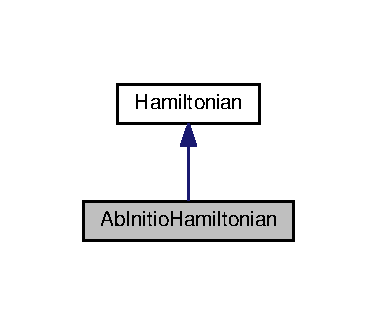
\includegraphics[width=181pt]{classAbInitioHamiltonian__inherit__graph}
\end{center}
\end{figure}


Collaboration diagram for Ab\+Initio\+Hamiltonian\+:\nopagebreak
\begin{figure}[H]
\begin{center}
\leavevmode
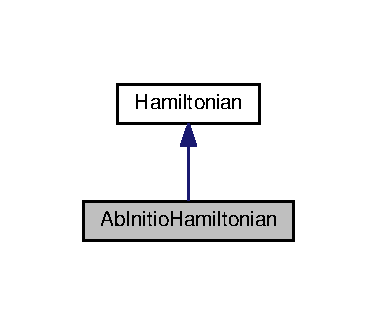
\includegraphics[width=181pt]{classAbInitioHamiltonian__coll__graph}
\end{center}
\end{figure}
\doxysubsection*{Public Member Functions}
\begin{DoxyCompactItemize}
\item 
\mbox{\Hypertarget{classAbInitioHamiltonian_a4aa129e13515a9d1b1d6fd659d36432f}\label{classAbInitioHamiltonian_a4aa129e13515a9d1b1d6fd659d36432f}} 
{\bfseries Ab\+Initio\+Hamiltonian} (const std\+::string \&fname)
\item 
\mbox{\Hypertarget{classAbInitioHamiltonian_a3d2a53be607a17c7f8461e5d9dd8380e}\label{classAbInitioHamiltonian_a3d2a53be607a17c7f8461e5d9dd8380e}} 
defs\+::ham\+\_\+t {\bfseries get\+\_\+element\+\_\+0} (const defs\+::det\+\_\+work \&occs, const size\+\_\+t \&nocc) const override
\item 
\mbox{\Hypertarget{classAbInitioHamiltonian_ade6591be81ad6f1b9604ae5fc66f6010}\label{classAbInitioHamiltonian_ade6591be81ad6f1b9604ae5fc66f6010}} 
defs\+::ham\+\_\+t {\bfseries get\+\_\+element\+\_\+1} (const \mbox{\hyperlink{classAntisymConnection}{Antisym\+Connection}} \&connection) const override
\item 
\mbox{\Hypertarget{classAbInitioHamiltonian_af8d0596a4876dd88db46eed075eba4c5}\label{classAbInitioHamiltonian_af8d0596a4876dd88db46eed075eba4c5}} 
defs\+::ham\+\_\+t {\bfseries get\+\_\+element\+\_\+2} (const size\+\_\+t \&i, const size\+\_\+t \&j, const size\+\_\+t \&k, const size\+\_\+t \&l) const override
\item 
\mbox{\Hypertarget{classAbInitioHamiltonian_a9e636c2c9e129d8c10ea909be3b04e7c}\label{classAbInitioHamiltonian_a9e636c2c9e129d8c10ea909be3b04e7c}} 
size\+\_\+t {\bfseries nelec} () const override
\item 
\mbox{\Hypertarget{classAbInitioHamiltonian_a929c348348755243865bf6a9c9e812cd}\label{classAbInitioHamiltonian_a929c348348755243865bf6a9c9e812cd}} 
bool {\bfseries spin\+\_\+resolved} () const override
\item 
\mbox{\Hypertarget{classAbInitioHamiltonian_af2917e415e826b1b647a22e023115eb3}\label{classAbInitioHamiltonian_af2917e415e826b1b647a22e023115eb3}} 
bool {\bfseries spin\+\_\+conserving} () const override
\item 
\mbox{\Hypertarget{classAbInitioHamiltonian_ae3ee97b2fa22a7153553170715593456}\label{classAbInitioHamiltonian_ae3ee97b2fa22a7153553170715593456}} 
const \mbox{\hyperlink{classIntegrals__1e}{Integrals\+\_\+1e}}$<$ defs\+::ham\+\_\+t, defs\+::isym\+\_\+1e $>$ \& {\bfseries int\+\_\+1} () const
\item 
\mbox{\Hypertarget{classAbInitioHamiltonian_ac123532bdab22e9e707f0b24963a4536}\label{classAbInitioHamiltonian_ac123532bdab22e9e707f0b24963a4536}} 
const \mbox{\hyperlink{classIntegrals__2e}{Integrals\+\_\+2e}}$<$ defs\+::ham\+\_\+t, defs\+::isym\+\_\+2e $>$ \& {\bfseries int\+\_\+2} () const
\item 
\mbox{\Hypertarget{classAbInitioHamiltonian_afed1192c0ee64815c60d11724347e723}\label{classAbInitioHamiltonian_afed1192c0ee64815c60d11724347e723}} 
virtual defs\+::ham\+\_\+t {\bfseries get\+\_\+element\+\_\+0} (const defs\+::det\+\_\+work \&occs, const size\+\_\+t \&nocc) const=0
\item 
\mbox{\Hypertarget{classAbInitioHamiltonian_a8944945ff8fe0ba62d39b0dfbe75ece6}\label{classAbInitioHamiltonian_a8944945ff8fe0ba62d39b0dfbe75ece6}} 
defs\+::ham\+\_\+t {\bfseries get\+\_\+element\+\_\+0} (const \mbox{\hyperlink{structOccupiedOrbitals}{Occupied\+Orbitals}} \&occs) const
\item 
\mbox{\Hypertarget{classAbInitioHamiltonian_aaf20ea0c5334bf7ff6248b888508856c}\label{classAbInitioHamiltonian_aaf20ea0c5334bf7ff6248b888508856c}} 
defs\+::ham\+\_\+t {\bfseries get\+\_\+element\+\_\+0} (const \mbox{\hyperlink{classDeterminantElement}{Determinant\+Element}} \&det) const
\item 
\mbox{\Hypertarget{classAbInitioHamiltonian_a829e544ae21fdd48056194a3d728a028}\label{classAbInitioHamiltonian_a829e544ae21fdd48056194a3d728a028}} 
defs\+::ham\+\_\+t {\bfseries get\+\_\+element\+\_\+0} (const \mbox{\hyperlink{classAntisymConnection}{Antisym\+Connection}} \&connection) const
\item 
\mbox{\Hypertarget{classAbInitioHamiltonian_a632617dc34ee846167e9876ea0087992}\label{classAbInitioHamiltonian_a632617dc34ee846167e9876ea0087992}} 
virtual defs\+::ham\+\_\+t {\bfseries get\+\_\+element\+\_\+1} (const \mbox{\hyperlink{classAntisymConnection}{Antisym\+Connection}} \&connection) const=0
\item 
\mbox{\Hypertarget{classAbInitioHamiltonian_a1b8a14989abd4ab25ed6732ef7094398}\label{classAbInitioHamiltonian_a1b8a14989abd4ab25ed6732ef7094398}} 
virtual defs\+::ham\+\_\+t {\bfseries get\+\_\+element\+\_\+2} (const size\+\_\+t \&i, const size\+\_\+t \&j, const size\+\_\+t \&k, const size\+\_\+t \&l) const=0
\item 
\mbox{\Hypertarget{classAbInitioHamiltonian_a82271a080e62d9a6b48dca4dec4d2e6c}\label{classAbInitioHamiltonian_a82271a080e62d9a6b48dca4dec4d2e6c}} 
defs\+::ham\+\_\+t {\bfseries get\+\_\+element\+\_\+2} (const \mbox{\hyperlink{classConnection}{Connection}} \&connection) const
\item 
\mbox{\Hypertarget{classAbInitioHamiltonian_a2c098a580ab7260fc092e4a8d5021e70}\label{classAbInitioHamiltonian_a2c098a580ab7260fc092e4a8d5021e70}} 
defs\+::ham\+\_\+t {\bfseries get\+\_\+element\+\_\+2} (const \mbox{\hyperlink{classAntisymConnection}{Antisym\+Connection}} \&connection) const
\end{DoxyCompactItemize}
\doxysubsection*{Additional Inherited Members}


The documentation for this class was generated from the following files\+:\begin{DoxyCompactItemize}
\item 
/home/teamcity/\+Team\+City/build\+Agent/work/5343cdffda4690e5/src/core/hamiltonian/Ab\+Initio\+Hamiltonian.\+h\item 
/home/teamcity/\+Team\+City/build\+Agent/work/5343cdffda4690e5/src/core/hamiltonian/Ab\+Initio\+Hamiltonian.\+cpp\end{DoxyCompactItemize}

\hypertarget{classAliaser}{}\section{Aliaser Class Reference}
\label{classAliaser}\index{Aliaser@{Aliaser}}
\subsection*{Public Member Functions}
\begin{DoxyCompactItemize}
\item 
{\bfseries Aliaser} (const size\+\_\+t nprob, \hyperlink{classPrivateStore}{Private\+Store}$<$ \hyperlink{classPRNG}{P\+R\+NG} $>$ \&prng)\hypertarget{classAliaser_aa5f5b86c6595e0d3871173907eca510d}{}\label{classAliaser_aa5f5b86c6595e0d3871173907eca510d}

\item 
void {\bfseries update} (const defs\+::prob\+\_\+t $\ast$probs, const size\+\_\+t nprob)\hypertarget{classAliaser_a889ee75afc2c656b24a738fd8f71a0a3}{}\label{classAliaser_a889ee75afc2c656b24a738fd8f71a0a3}

\item 
void {\bfseries update} (const std\+::vector$<$ defs\+::prob\+\_\+t $>$ \&probs)\hypertarget{classAliaser_a701ef3f3e90a68a0cda812d2b3114b9e}{}\label{classAliaser_a701ef3f3e90a68a0cda812d2b3114b9e}

\item 
{\bfseries Aliaser} (const defs\+::prob\+\_\+t $\ast$probs, const size\+\_\+t nprob, \hyperlink{classPrivateStore}{Private\+Store}$<$ \hyperlink{classPRNG}{P\+R\+NG} $>$ \&prng)\hypertarget{classAliaser_aebe3aeea847f0e64a9d5d9d115939ca5}{}\label{classAliaser_aebe3aeea847f0e64a9d5d9d115939ca5}

\item 
{\bfseries Aliaser} (const std\+::vector$<$ defs\+::prob\+\_\+t $>$ \&probs, const size\+\_\+t nprob, \hyperlink{classPrivateStore}{Private\+Store}$<$ \hyperlink{classPRNG}{P\+R\+NG} $>$ \&prng)\hypertarget{classAliaser_aace600d68d2e1a8d7c3f56a75465cd1f}{}\label{classAliaser_aace600d68d2e1a8d7c3f56a75465cd1f}

\item 
{\bfseries Aliaser} (const std\+::vector$<$ defs\+::prob\+\_\+t $>$ \&probs, \hyperlink{classPrivateStore}{Private\+Store}$<$ \hyperlink{classPRNG}{P\+R\+NG} $>$ \&prng)\hypertarget{classAliaser_a54050a9dcb6cb807837a63bece7e7453}{}\label{classAliaser_a54050a9dcb6cb807837a63bece7e7453}

\item 
size\+\_\+t {\bfseries draw} () const \hypertarget{classAliaser_a767b8402017e59b6a8e242a07006adda}{}\label{classAliaser_a767b8402017e59b6a8e242a07006adda}

\item 
defs\+::prob\+\_\+t {\bfseries norm} () const \hypertarget{classAliaser_a07412197898076fcbf7e5a9679722f33}{}\label{classAliaser_a07412197898076fcbf7e5a9679722f33}

\item 
defs\+::prob\+\_\+t {\bfseries prob} (const size\+\_\+t \&i) const \hypertarget{classAliaser_ade32f8b7ca75b5ad28c5133c6b4b64a8}{}\label{classAliaser_ade32f8b7ca75b5ad28c5133c6b4b64a8}

\end{DoxyCompactItemize}


The documentation for this class was generated from the following file\+:\begin{DoxyCompactItemize}
\item 
/home/teamcity/\+Team\+City/build\+Agent/work/5343cdffda4690e5/src/core/sample/Aliaser.\+h\end{DoxyCompactItemize}

\hypertarget{classAlignedAllocator}{}\doxysection{Aligned\+Allocator$<$ T, alignment $>$ Class Template Reference}
\label{classAlignedAllocator}\index{AlignedAllocator$<$ T, alignment $>$@{AlignedAllocator$<$ T, alignment $>$}}
\doxysubsection*{Classes}
\begin{DoxyCompactItemize}
\item 
struct \mbox{\hyperlink{structAlignedAllocator_1_1rebind}{rebind}}
\end{DoxyCompactItemize}
\doxysubsection*{Public Types}
\begin{DoxyCompactItemize}
\item 
\mbox{\Hypertarget{classAlignedAllocator_a8156c3bcb3f481eee1ed5744f1bee588}\label{classAlignedAllocator_a8156c3bcb3f481eee1ed5744f1bee588}} 
typedef T {\bfseries value\+\_\+type}
\item 
\mbox{\Hypertarget{classAlignedAllocator_ace173cbb585102f35337af6a2f0773d0}\label{classAlignedAllocator_ace173cbb585102f35337af6a2f0773d0}} 
typedef T $\ast$ {\bfseries pointer}
\item 
\mbox{\Hypertarget{classAlignedAllocator_aa0023d9d0cd46d1436908ca3438b4253}\label{classAlignedAllocator_aa0023d9d0cd46d1436908ca3438b4253}} 
typedef const T $\ast$ {\bfseries const\+\_\+pointer}
\item 
\mbox{\Hypertarget{classAlignedAllocator_aa7ea4f8ae44e6681548689059258f7ed}\label{classAlignedAllocator_aa7ea4f8ae44e6681548689059258f7ed}} 
typedef T \& {\bfseries reference}
\item 
\mbox{\Hypertarget{classAlignedAllocator_a1f9389d4b2f98606022504b1695945b7}\label{classAlignedAllocator_a1f9389d4b2f98606022504b1695945b7}} 
typedef const T \& {\bfseries const\+\_\+reference}
\item 
\mbox{\Hypertarget{classAlignedAllocator_ab6e51b4656a9e595dce6cb55d5386aac}\label{classAlignedAllocator_ab6e51b4656a9e595dce6cb55d5386aac}} 
typedef std\+::size\+\_\+t {\bfseries size\+\_\+type}
\end{DoxyCompactItemize}
\doxysubsection*{Public Member Functions}
\begin{DoxyCompactItemize}
\item 
\mbox{\Hypertarget{classAlignedAllocator_a3dcd9387b99c16c540567a5a1ab1e1bf}\label{classAlignedAllocator_a3dcd9387b99c16c540567a5a1ab1e1bf}} 
pointer {\bfseries address} (reference value) const
\item 
\mbox{\Hypertarget{classAlignedAllocator_a15c09625b168755a167d51dc0eebe610}\label{classAlignedAllocator_a15c09625b168755a167d51dc0eebe610}} 
const\+\_\+pointer {\bfseries address} (const\+\_\+reference value) const
\item 
\mbox{\Hypertarget{classAlignedAllocator_aefcbc30120c4a8080a04cb0256ccbd94}\label{classAlignedAllocator_aefcbc30120c4a8080a04cb0256ccbd94}} 
{\bfseries Aligned\+Allocator} (const \mbox{\hyperlink{classAlignedAllocator}{Aligned\+Allocator}} \&alloc)  throw ()
\item 
\mbox{\Hypertarget{classAlignedAllocator_a99d45b93a0a0e7a229cc0c1b954f21f0}\label{classAlignedAllocator_a99d45b93a0a0e7a229cc0c1b954f21f0}} 
{\footnotesize template$<$class U $>$ }\\{\bfseries Aligned\+Allocator} (const \mbox{\hyperlink{classAlignedAllocator}{Aligned\+Allocator}}$<$ U, alignment $>$ \&)  throw ()
\item 
\mbox{\Hypertarget{classAlignedAllocator_abb485ea66e2850b16b782b64827115f4}\label{classAlignedAllocator_abb485ea66e2850b16b782b64827115f4}} 
size\+\_\+type {\bfseries max\+\_\+size} () const  throw ()
\item 
\mbox{\Hypertarget{classAlignedAllocator_afaa32dfd9b767ceccba057b0fdf9e8b9}\label{classAlignedAllocator_afaa32dfd9b767ceccba057b0fdf9e8b9}} 
pointer {\bfseries allocate} (size\+\_\+type num, const void $\ast$=0)
\item 
\mbox{\Hypertarget{classAlignedAllocator_a9c352b5d0c908f15d869b2555211d6eb}\label{classAlignedAllocator_a9c352b5d0c908f15d869b2555211d6eb}} 
void {\bfseries construct} (pointer p, const T \&value)
\item 
\mbox{\Hypertarget{classAlignedAllocator_a46bb788a20e8166d20ccd4e3f47e48b1}\label{classAlignedAllocator_a46bb788a20e8166d20ccd4e3f47e48b1}} 
void {\bfseries destroy} (pointer p)
\item 
\mbox{\Hypertarget{classAlignedAllocator_afcdd0473a1bf2cd63800b047d8d540ae}\label{classAlignedAllocator_afcdd0473a1bf2cd63800b047d8d540ae}} 
void {\bfseries deallocate} (pointer p, size\+\_\+type num)
\end{DoxyCompactItemize}


The documentation for this class was generated from the following file\+:\begin{DoxyCompactItemize}
\item 
/home/teamcity/\+Team\+City/build\+Agent/work/5343cdffda4690e5/src/core/thread/Aligned\+Allocator.\+h\end{DoxyCompactItemize}

\hypertarget{classAlignedAllocator2}{}\section{Aligned\+Allocator2$<$ T, alignment $>$ Class Template Reference}
\label{classAlignedAllocator2}\index{Aligned\+Allocator2$<$ T, alignment $>$@{Aligned\+Allocator2$<$ T, alignment $>$}}
\subsection*{Classes}
\begin{DoxyCompactItemize}
\item 
struct \hyperlink{structAlignedAllocator2_1_1rebind}{rebind}
\end{DoxyCompactItemize}
\subsection*{Public Types}
\begin{DoxyCompactItemize}
\item 
typedef T {\bfseries value\+\_\+type}\hypertarget{classAlignedAllocator2_a7f734b30cdc7bbfb0f519a278da1870a}{}\label{classAlignedAllocator2_a7f734b30cdc7bbfb0f519a278da1870a}

\item 
typedef T $\ast$ {\bfseries pointer}\hypertarget{classAlignedAllocator2_a02d4fa089bf1bd3e50a1c0612c556fd0}{}\label{classAlignedAllocator2_a02d4fa089bf1bd3e50a1c0612c556fd0}

\item 
typedef const T $\ast$ {\bfseries const\+\_\+pointer}\hypertarget{classAlignedAllocator2_a5c47a855c95ef33c3eeca37f0959e815}{}\label{classAlignedAllocator2_a5c47a855c95ef33c3eeca37f0959e815}

\item 
typedef T \& {\bfseries reference}\hypertarget{classAlignedAllocator2_ae38927ee51e59fdbac9bde00a610c430}{}\label{classAlignedAllocator2_ae38927ee51e59fdbac9bde00a610c430}

\item 
typedef const T \& {\bfseries const\+\_\+reference}\hypertarget{classAlignedAllocator2_a40539bddb4e989d0f91a7afc25aa9b9d}{}\label{classAlignedAllocator2_a40539bddb4e989d0f91a7afc25aa9b9d}

\item 
typedef std\+::size\+\_\+t {\bfseries size\+\_\+type}\hypertarget{classAlignedAllocator2_aa9d3b748c6513be70b0e79922b295379}{}\label{classAlignedAllocator2_aa9d3b748c6513be70b0e79922b295379}

\item 
typedef std\+::ptrdiff\+\_\+t {\bfseries difference\+\_\+type}\hypertarget{classAlignedAllocator2_af30a7f0cdea6d7b9fd81bf33365b4de4}{}\label{classAlignedAllocator2_af30a7f0cdea6d7b9fd81bf33365b4de4}

\end{DoxyCompactItemize}
\subsection*{Public Member Functions}
\begin{DoxyCompactItemize}
\item 
pointer {\bfseries address} (reference value) const \hypertarget{classAlignedAllocator2_aa8c6c6d9675b6c5132f4039e45335fcd}{}\label{classAlignedAllocator2_aa8c6c6d9675b6c5132f4039e45335fcd}

\item 
const\+\_\+pointer {\bfseries address} (const\+\_\+reference value) const \hypertarget{classAlignedAllocator2_af26b687ed65dd994fa650fbffed38189}{}\label{classAlignedAllocator2_af26b687ed65dd994fa650fbffed38189}

\item 
{\bfseries Aligned\+Allocator2} (const \hyperlink{classAlignedAllocator2}{Aligned\+Allocator2} \&)  throw ()\hypertarget{classAlignedAllocator2_a055b6aee6d67fa9ef19b945831af6ba2}{}\label{classAlignedAllocator2_a055b6aee6d67fa9ef19b945831af6ba2}

\item 
{\footnotesize template$<$class U $>$ }\\{\bfseries Aligned\+Allocator2} (const \hyperlink{classAlignedAllocator2}{Aligned\+Allocator2}$<$ U, alignment $>$ \&)  throw ()\hypertarget{classAlignedAllocator2_a9baed24dface5d93594192f80011a22b}{}\label{classAlignedAllocator2_a9baed24dface5d93594192f80011a22b}

\item 
size\+\_\+type {\bfseries max\+\_\+size} () const   throw ()\hypertarget{classAlignedAllocator2_a62217df2c44663d5013e411d8b284905}{}\label{classAlignedAllocator2_a62217df2c44663d5013e411d8b284905}

\item 
pointer {\bfseries allocate} (size\+\_\+type num, const void $\ast$=0)\hypertarget{classAlignedAllocator2_a50ebd094568307b1d334c051a6c4452e}{}\label{classAlignedAllocator2_a50ebd094568307b1d334c051a6c4452e}

\item 
void {\bfseries construct} (pointer p, const T \&value)\hypertarget{classAlignedAllocator2_a53dbcd7925c1b6d9f5a77021aca6d90b}{}\label{classAlignedAllocator2_a53dbcd7925c1b6d9f5a77021aca6d90b}

\item 
void {\bfseries destroy} (pointer p)\hypertarget{classAlignedAllocator2_af1923df8d69d43050a6a98ec1994ee58}{}\label{classAlignedAllocator2_af1923df8d69d43050a6a98ec1994ee58}

\item 
void {\bfseries deallocate} (pointer p, size\+\_\+type num)\hypertarget{classAlignedAllocator2_ac1e8dd1ef4fbd9f2ddb182bbac864e49}{}\label{classAlignedAllocator2_ac1e8dd1ef4fbd9f2ddb182bbac864e49}

\end{DoxyCompactItemize}


The documentation for this class was generated from the following file\+:\begin{DoxyCompactItemize}
\item 
/home/teamcity/\+Team\+City/build\+Agent/work/5343cdffda4690e5/src/core/thread/Aligned\+Allocator2.\+h\end{DoxyCompactItemize}

\hypertarget{classDeterminantElement_1_1AntiDatawordEnumerator}{}\section{Determinant\+Element\+:\+:Anti\+Dataword\+Enumerator Class Reference}
\label{classDeterminantElement_1_1AntiDatawordEnumerator}\index{Determinant\+Element\+::\+Anti\+Dataword\+Enumerator@{Determinant\+Element\+::\+Anti\+Dataword\+Enumerator}}


Inheritance diagram for Determinant\+Element\+:\+:Anti\+Dataword\+Enumerator\+:
% FIG 0


Collaboration diagram for Determinant\+Element\+:\+:Anti\+Dataword\+Enumerator\+:
% FIG 1
\subsection*{Public Member Functions}
\begin{DoxyCompactItemize}
\item 
{\bfseries Anti\+Dataword\+Enumerator} (const \hyperlink{classDeterminantElement}{Determinant\+Element} \&data)\hypertarget{classDeterminantElement_1_1AntiDatawordEnumerator_a09e78d2e57f66b5b7186ac7979c877ba}{}\label{classDeterminantElement_1_1AntiDatawordEnumerator_a09e78d2e57f66b5b7186ac7979c877ba}

\end{DoxyCompactItemize}
\subsection*{Additional Inherited Members}


The documentation for this class was generated from the following files\+:\begin{DoxyCompactItemize}
\item 
/home/teamcity/\+Team\+City/build\+Agent/work/5343cdffda4690e5/src/core/table/Determinant\+Field.\+h\item 
/home/teamcity/\+Team\+City/build\+Agent/work/5343cdffda4690e5/src/core/table/Determinant\+Field.\+cpp\end{DoxyCompactItemize}

\hypertarget{classAntisymConnection}{}\section{Antisym\+Connection Class Reference}
\label{classAntisymConnection}\index{Antisym\+Connection@{Antisym\+Connection}}


Inheritance diagram for Antisym\+Connection\+:\nopagebreak
\begin{figure}[H]
\begin{center}
\leavevmode
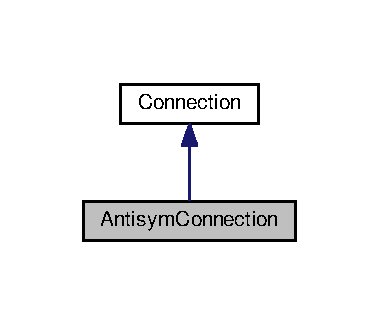
\includegraphics[width=182pt]{classAntisymConnection__inherit__graph}
\end{center}
\end{figure}


Collaboration diagram for Antisym\+Connection\+:\nopagebreak
\begin{figure}[H]
\begin{center}
\leavevmode
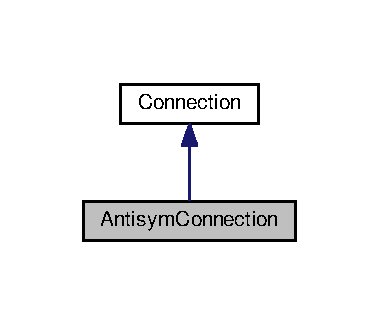
\includegraphics[width=182pt]{classAntisymConnection__coll__graph}
\end{center}
\end{figure}
\subsection*{Public Member Functions}
\begin{DoxyCompactItemize}
\item 
{\bfseries Antisym\+Connection} (const \hyperlink{classField}{Field} $\ast$field)\hypertarget{classAntisymConnection_aaee6b6954a7a024a68f648652447f6b0}{}\label{classAntisymConnection_aaee6b6954a7a024a68f648652447f6b0}

\item 
{\bfseries Antisym\+Connection} (const \hyperlink{classDeterminantElement}{Determinant\+Element} \&ket, const \hyperlink{classDeterminantElement}{Determinant\+Element} \&bra)\hypertarget{classAntisymConnection_ac340ada066d7220944961e6fd815419e}{}\label{classAntisymConnection_ac340ada066d7220944961e6fd815419e}

\item 
{\bfseries Antisym\+Connection} (const \hyperlink{classDeterminantElement}{Determinant\+Element} \&ket)\hypertarget{classAntisymConnection_a4efe834c774fe0537dd85fa83801dd18}{}\label{classAntisymConnection_a4efe834c774fe0537dd85fa83801dd18}

\item 
void {\bfseries connect} (const \hyperlink{classDeterminantElement}{Determinant\+Element} \&ket, const \hyperlink{classDeterminantElement}{Determinant\+Element} \&bra) override\hypertarget{classAntisymConnection_a6c4fac9e367a748774108d4da5d8f3f8}{}\label{classAntisymConnection_a6c4fac9e367a748774108d4da5d8f3f8}

\item 
void {\bfseries apply} (const \hyperlink{classDeterminantElement}{Determinant\+Element} \&ket)\hypertarget{classAntisymConnection_a0eb1b8853be6cd73b8f1d6b488915c1b}{}\label{classAntisymConnection_a0eb1b8853be6cd73b8f1d6b488915c1b}

\item 
void {\bfseries apply} (const \hyperlink{classDeterminantElement}{Determinant\+Element} \&ket, \hyperlink{classDeterminantElement}{Determinant\+Element} \&bra) override\hypertarget{classAntisymConnection_a987a278b67158864215ef48f7d17f3e8}{}\label{classAntisymConnection_a987a278b67158864215ef48f7d17f3e8}

\item 
const defs\+::det\+\_\+work \& {\bfseries com} () const \hypertarget{classAntisymConnection_a7ea22c794cd53aba127c6c8f04fa4455}{}\label{classAntisymConnection_a7ea22c794cd53aba127c6c8f04fa4455}

\item 
const size\+\_\+t \& {\bfseries com} (const size\+\_\+t \&i) const \hypertarget{classAntisymConnection_a09288e7bcefd06caabefd93448322ff3}{}\label{classAntisymConnection_a09288e7bcefd06caabefd93448322ff3}

\item 
const size\+\_\+t \& {\bfseries ncom} () const \hypertarget{classAntisymConnection_a458ecaa28eb699e7b9594e73e81780be}{}\label{classAntisymConnection_a458ecaa28eb699e7b9594e73e81780be}

\item 
const bool \& {\bfseries phase} () const \hypertarget{classAntisymConnection_aefb3cefa46b0fe2c9b58f47d795ce1de}{}\label{classAntisymConnection_aefb3cefa46b0fe2c9b58f47d795ce1de}

\end{DoxyCompactItemize}
\subsection*{Additional Inherited Members}


The documentation for this class was generated from the following files\+:\begin{DoxyCompactItemize}
\item 
/home/teamcity/\+Team\+City/build\+Agent/work/5343cdffda4690e5/src/core/fermion/Connection.\+h\item 
/home/teamcity/\+Team\+City/build\+Agent/work/5343cdffda4690e5/src/core/fermion/Connection.\+cpp\end{DoxyCompactItemize}

\hypertarget{classArrayIndexer}{}\doxysection{Array\+Indexer$<$ nind $>$ Class Template Reference}
\label{classArrayIndexer}\index{ArrayIndexer$<$ nind $>$@{ArrayIndexer$<$ nind $>$}}
\doxysubsection*{Public Member Functions}
\begin{DoxyCompactItemize}
\item 
\mbox{\Hypertarget{classArrayIndexer_ad9b60dd97a659e98714086e590fb5b5b}\label{classArrayIndexer_ad9b60dd97a659e98714086e590fb5b5b}} 
{\bfseries Array\+Indexer} (const std\+::array$<$ size\+\_\+t, nind $>$ \&shape)
\item 
\mbox{\Hypertarget{classArrayIndexer_ad8c40e76670adb49e8b437e8762fee7f}\label{classArrayIndexer_ad8c40e76670adb49e8b437e8762fee7f}} 
const std\+::array$<$ size\+\_\+t, nind $>$ \& {\bfseries shape} () const
\item 
\mbox{\Hypertarget{classArrayIndexer_a61c06b2d2d0d268f8583397ec920eb40}\label{classArrayIndexer_a61c06b2d2d0d268f8583397ec920eb40}} 
const std\+::array$<$ size\+\_\+t, nind $>$ \& {\bfseries strides} () const
\item 
\mbox{\Hypertarget{classArrayIndexer_af89ed824c30a5037c5d6ef41fac2268b}\label{classArrayIndexer_af89ed824c30a5037c5d6ef41fac2268b}} 
size\+\_\+t {\bfseries nelement} () const
\item 
\mbox{\Hypertarget{classArrayIndexer_acd9add8f9581955506f7d5a0992b52b9}\label{classArrayIndexer_acd9add8f9581955506f7d5a0992b52b9}} 
bool {\bfseries operator==} (const \mbox{\hyperlink{classArrayIndexer}{Array\+Indexer}} \&rhs) const
\item 
\mbox{\Hypertarget{classArrayIndexer_a2c464ee209d40a7da2d9b20f9a84e1d4}\label{classArrayIndexer_a2c464ee209d40a7da2d9b20f9a84e1d4}} 
bool {\bfseries operator!=} (const \mbox{\hyperlink{classArrayIndexer}{Array\+Indexer}} \&rhs) const
\item 
\mbox{\Hypertarget{classArrayIndexer_ad9cc48aefed1932ada32f788882ec5a1}\label{classArrayIndexer_ad9cc48aefed1932ada32f788882ec5a1}} 
size\+\_\+t {\bfseries get} (const std\+::array$<$ size\+\_\+t, nind $>$ \&inds) const
\end{DoxyCompactItemize}
\doxysubsection*{Protected Attributes}
\begin{DoxyCompactItemize}
\item 
\mbox{\Hypertarget{classArrayIndexer_ae9f32843d8e8cb73a1d6034be9ea45fb}\label{classArrayIndexer_ae9f32843d8e8cb73a1d6034be9ea45fb}} 
std\+::array$<$ size\+\_\+t, nind $>$ {\bfseries m\+\_\+shape} \{\}
\item 
\mbox{\Hypertarget{classArrayIndexer_a6462c050c22291cdc1e76ff7ece5e918}\label{classArrayIndexer_a6462c050c22291cdc1e76ff7ece5e918}} 
std\+::array$<$ size\+\_\+t, nind $>$ {\bfseries m\+\_\+strides} \{\}
\end{DoxyCompactItemize}


The documentation for this class was generated from the following file\+:\begin{DoxyCompactItemize}
\item 
/home/teamcity/\+Team\+City/build\+Agent/work/5343cdffda4690e5/src/core/multidim/Array\+Indexer.\+h\end{DoxyCompactItemize}

\hypertarget{structAtomic}{}\section{Atomic$<$ T $>$ Struct Template Reference}
\label{structAtomic}\index{Atomic$<$ T $>$@{Atomic$<$ T $>$}}
\subsection*{Public Member Functions}
\begin{DoxyCompactItemize}
\item 
{\bfseries Atomic} (T \&v)\hypertarget{structAtomic_a2997eca4631493cb3d5f7bbd02012517}{}\label{structAtomic_a2997eca4631493cb3d5f7bbd02012517}

\item 
T \& {\bfseries operator+=} (const T \&rhs)\hypertarget{structAtomic_a1d06a25a2b3a44a9f575030b02dacf41}{}\label{structAtomic_a1d06a25a2b3a44a9f575030b02dacf41}

\item 
T \& {\bfseries operator-\/=} (const T \&rhs)\hypertarget{structAtomic_a9b698d00b94a57bd04ecc1d4aa406e7a}{}\label{structAtomic_a9b698d00b94a57bd04ecc1d4aa406e7a}

\item 
T \& {\bfseries operator$\ast$=} (const T \&rhs)\hypertarget{structAtomic_a3453eac863d6fae62b20d1b0b6bbcc75}{}\label{structAtomic_a3453eac863d6fae62b20d1b0b6bbcc75}

\item 
T \& {\bfseries operator/=} (const T \&rhs)\hypertarget{structAtomic_aa9143d0b7becfb0f724a24be3dc2ef4a}{}\label{structAtomic_aa9143d0b7becfb0f724a24be3dc2ef4a}

\end{DoxyCompactItemize}
\subsection*{Public Attributes}
\begin{DoxyCompactItemize}
\item 
T \& {\bfseries m\+\_\+v}\hypertarget{structAtomic_ab31f90d99eb45d5305f7d19cb8d2ea6e}{}\label{structAtomic_ab31f90d99eb45d5305f7d19cb8d2ea6e}

\end{DoxyCompactItemize}


The documentation for this struct was generated from the following file\+:\begin{DoxyCompactItemize}
\item 
/home/teamcity/\+Team\+City/build\+Agent/work/5343cdffda4690e5/src/core/thread/Atomic.\+h\end{DoxyCompactItemize}

\hypertarget{structAtomic_3_01bool_01_4}{}\section{Atomic$<$ bool $>$ Struct Template Reference}
\label{structAtomic_3_01bool_01_4}\index{Atomic$<$ bool $>$@{Atomic$<$ bool $>$}}
\subsection*{Public Member Functions}
\begin{DoxyCompactItemize}
\item 
{\bfseries Atomic} (bool \&v)\hypertarget{structAtomic_3_01bool_01_4_a5cf338584c4fb42d13e90f116824620a}{}\label{structAtomic_3_01bool_01_4_a5cf338584c4fb42d13e90f116824620a}

\item 
bool \& {\bfseries operator\&=} (const bool \&rhs)\hypertarget{structAtomic_3_01bool_01_4_a996a6fb829239e38c8cffbcbda4aa4a3}{}\label{structAtomic_3_01bool_01_4_a996a6fb829239e38c8cffbcbda4aa4a3}

\item 
bool \& {\bfseries operator$\vert$=} (const bool \&rhs)\hypertarget{structAtomic_3_01bool_01_4_ae6e0b36f7eb450522e50524c1bd8a941}{}\label{structAtomic_3_01bool_01_4_ae6e0b36f7eb450522e50524c1bd8a941}

\end{DoxyCompactItemize}
\subsection*{Public Attributes}
\begin{DoxyCompactItemize}
\item 
bool \& {\bfseries m\+\_\+v}\hypertarget{structAtomic_3_01bool_01_4_a1457dd7ca19855645abcd2230ae43d91}{}\label{structAtomic_3_01bool_01_4_a1457dd7ca19855645abcd2230ae43d91}

\end{DoxyCompactItemize}


The documentation for this struct was generated from the following file\+:\begin{DoxyCompactItemize}
\item 
/home/teamcity/\+Team\+City/build\+Agent/work/5343cdffda4690e5/src/core/thread/Atomic.\+h\end{DoxyCompactItemize}

\hypertarget{structAtomic_3_01std_1_1complex_3_01T_01_4_01_4}{}\doxysection{Atomic$<$ std\+::complex$<$ T $>$ $>$ Struct Template Reference}
\label{structAtomic_3_01std_1_1complex_3_01T_01_4_01_4}\index{Atomic$<$ std::complex$<$ T $>$ $>$@{Atomic$<$ std::complex$<$ T $>$ $>$}}
\doxysubsection*{Public Member Functions}
\begin{DoxyCompactItemize}
\item 
\mbox{\Hypertarget{structAtomic_3_01std_1_1complex_3_01T_01_4_01_4_a429172c84e33b68d55b3daa4aa76de2e}\label{structAtomic_3_01std_1_1complex_3_01T_01_4_01_4_a429172c84e33b68d55b3daa4aa76de2e}} 
{\bfseries Atomic} (std\+::complex$<$ T $>$ \&v)
\item 
\mbox{\Hypertarget{structAtomic_3_01std_1_1complex_3_01T_01_4_01_4_ab8b6ae61c3a7f429aad583b984bc7cb2}\label{structAtomic_3_01std_1_1complex_3_01T_01_4_01_4_ab8b6ae61c3a7f429aad583b984bc7cb2}} 
std\+::complex$<$ T $>$ \& {\bfseries operator+=} (const std\+::complex$<$ T $>$ \&rhs)
\item 
\mbox{\Hypertarget{structAtomic_3_01std_1_1complex_3_01T_01_4_01_4_a8efe7bb5d46bb2c99c9f64a8947936d0}\label{structAtomic_3_01std_1_1complex_3_01T_01_4_01_4_a8efe7bb5d46bb2c99c9f64a8947936d0}} 
std\+::complex$<$ T $>$ \& {\bfseries operator-\/=} (const std\+::complex$<$ T $>$ \&rhs)
\item 
\mbox{\Hypertarget{structAtomic_3_01std_1_1complex_3_01T_01_4_01_4_a8bee8f433212391e736d5ca3d8394e0e}\label{structAtomic_3_01std_1_1complex_3_01T_01_4_01_4_a8bee8f433212391e736d5ca3d8394e0e}} 
std\+::complex$<$ T $>$ \& {\bfseries operator$\ast$=} (const std\+::complex$<$ T $>$ \&rhs)
\item 
\mbox{\Hypertarget{structAtomic_3_01std_1_1complex_3_01T_01_4_01_4_a28a8aeb205c2206abc0b0e67a0ffa322}\label{structAtomic_3_01std_1_1complex_3_01T_01_4_01_4_a28a8aeb205c2206abc0b0e67a0ffa322}} 
std\+::complex$<$ T $>$ \& {\bfseries operator/=} (const std\+::complex$<$ T $>$ \&rhs)
\end{DoxyCompactItemize}
\doxysubsection*{Public Attributes}
\begin{DoxyCompactItemize}
\item 
\mbox{\Hypertarget{structAtomic_3_01std_1_1complex_3_01T_01_4_01_4_a9def64112ed5fdbbbd8ed139299d118a}\label{structAtomic_3_01std_1_1complex_3_01T_01_4_01_4_a9def64112ed5fdbbbd8ed139299d118a}} 
T \& {\bfseries m\+\_\+real}
\item 
\mbox{\Hypertarget{structAtomic_3_01std_1_1complex_3_01T_01_4_01_4_a208d83261b1bdba3c17f40e37988f0da}\label{structAtomic_3_01std_1_1complex_3_01T_01_4_01_4_a208d83261b1bdba3c17f40e37988f0da}} 
T \& {\bfseries m\+\_\+imag}
\end{DoxyCompactItemize}


The documentation for this struct was generated from the following file\+:\begin{DoxyCompactItemize}
\item 
/home/teamcity/\+Team\+City/build\+Agent/work/5343cdffda4690e5/src/core/thread/Atomic.\+h\end{DoxyCompactItemize}

\hypertarget{classBitset}{}\section{Bitset Class Reference}
\label{classBitset}\index{Bitset@{Bitset}}


Inheritance diagram for Bitset\+:
\nopagebreak
\begin{figure}[H]
\begin{center}
\leavevmode
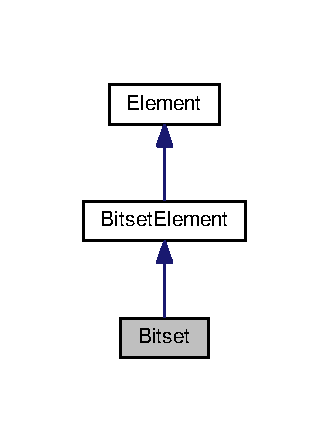
\includegraphics[width=158pt]{classBitset__inherit__graph}
\end{center}
\end{figure}


Collaboration diagram for Bitset\+:
\nopagebreak
\begin{figure}[H]
\begin{center}
\leavevmode
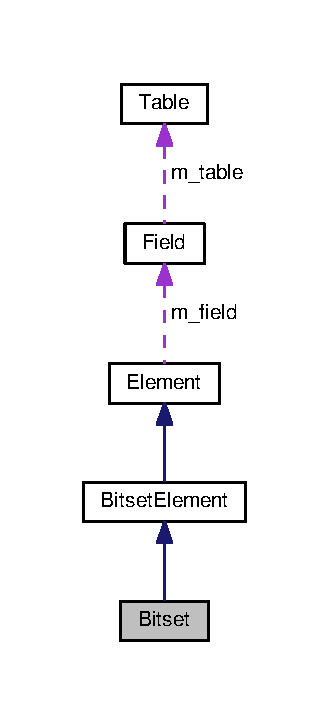
\includegraphics[width=158pt]{classBitset__coll__graph}
\end{center}
\end{figure}
\subsection*{Public Member Functions}
\begin{DoxyCompactItemize}
\item 
{\bfseries Bitset} (size\+\_\+t nbit)\hypertarget{classBitset_abfc9f780afcf5f1595320db5b3a8a51a}{}\label{classBitset_abfc9f780afcf5f1595320db5b3a8a51a}

\end{DoxyCompactItemize}
\subsection*{Additional Inherited Members}


The documentation for this class was generated from the following file\+:\begin{DoxyCompactItemize}
\item 
/home/teamcity/\+Team\+City/build\+Agent/work/5343cdffda4690e5/src/core/table/Bitset.\+h\end{DoxyCompactItemize}

\hypertarget{classBitsetClrEnumerator}{}\section{Bitset\+Clr\+Enumerator Class Reference}
\label{classBitsetClrEnumerator}\index{Bitset\+Clr\+Enumerator@{Bitset\+Clr\+Enumerator}}


Inheritance diagram for Bitset\+Clr\+Enumerator\+:
% FIG 0


Collaboration diagram for Bitset\+Clr\+Enumerator\+:
% FIG 1
\subsection*{Public Member Functions}
\begin{DoxyCompactItemize}
\item 
{\bfseries Bitset\+Clr\+Enumerator} (const \hyperlink{classBitsetElement}{Bitset\+Element} \&data1, \hyperlink{classEnumerator}{Enumerator}$<$ size\+\_\+t $>$ $\ast$subsequent=nullptr, size\+\_\+t offset=0)\hypertarget{classBitsetClrEnumerator_ac7b5a979fa9212e62c033848a81ddc7c}{}\label{classBitsetClrEnumerator_ac7b5a979fa9212e62c033848a81ddc7c}

\end{DoxyCompactItemize}
\subsection*{Additional Inherited Members}


The documentation for this class was generated from the following file\+:\begin{DoxyCompactItemize}
\item 
/home/teamcity/\+Team\+City/build\+Agent/work/5343cdffda4690e5/src/core/enumerator/Bitset\+Enumerator.\+h\end{DoxyCompactItemize}

\hypertarget{classBitsetElement}{}\doxysection{Bitset\+Element Class Reference}
\label{classBitsetElement}\index{BitsetElement@{BitsetElement}}


Inheritance diagram for Bitset\+Element\+:\nopagebreak
\begin{figure}[H]
\begin{center}
\leavevmode
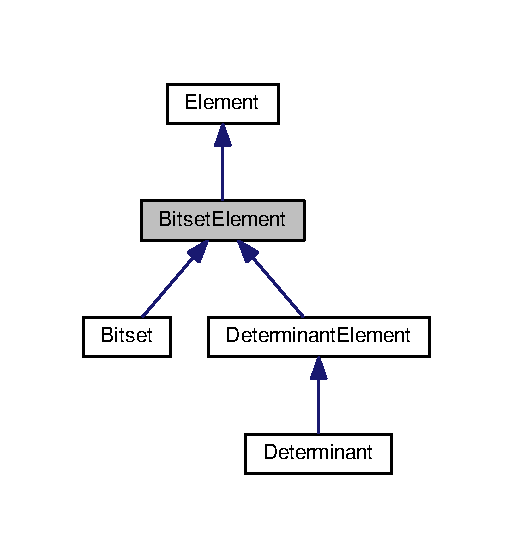
\includegraphics[width=246pt]{classBitsetElement__inherit__graph}
\end{center}
\end{figure}


Collaboration diagram for Bitset\+Element\+:\nopagebreak
\begin{figure}[H]
\begin{center}
\leavevmode
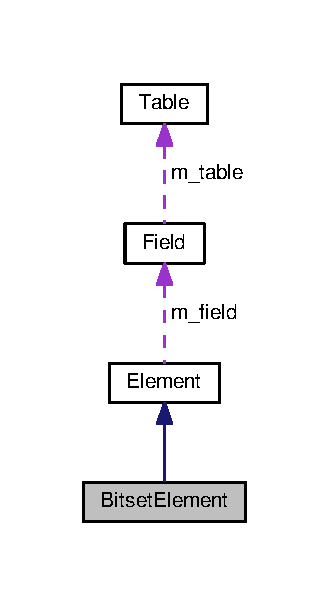
\includegraphics[width=158pt]{classBitsetElement__coll__graph}
\end{center}
\end{figure}
\doxysubsection*{Public Types}
\begin{DoxyCompactItemize}
\item 
\mbox{\Hypertarget{classBitsetElement_ac6669f289b7f7793033b515911a89ff2}\label{classBitsetElement_ac6669f289b7f7793033b515911a89ff2}} 
typedef \mbox{\hyperlink{classBitsetField}{Bitset\+Field}} {\bfseries Field\+\_\+T}
\end{DoxyCompactItemize}
\doxysubsection*{Public Member Functions}
\begin{DoxyCompactItemize}
\item 
\mbox{\Hypertarget{classBitsetElement_a84dd9f9e7dc0e559cdffe848f4dbd0f6}\label{classBitsetElement_a84dd9f9e7dc0e559cdffe848f4dbd0f6}} 
{\bfseries Bitset\+Element} (\mbox{\hyperlink{classBitsetField}{Bitset\+Field}} $\ast$field, char $\ast$begin)
\item 
\mbox{\Hypertarget{classBitsetElement_aed98af5268c63c2859507472e50c24af}\label{classBitsetElement_aed98af5268c63c2859507472e50c24af}} 
void {\bfseries set} (const defs\+::pair \&pair)
\item 
\mbox{\Hypertarget{classBitsetElement_a3997088e469e8235766eafbda0170cae}\label{classBitsetElement_a3997088e469e8235766eafbda0170cae}} 
virtual void {\bfseries set} (const size\+\_\+t \&ibit)
\item 
\mbox{\Hypertarget{classBitsetElement_aeb2427fdcfc7f1535ace3ae7bb2bdfa4}\label{classBitsetElement_aeb2427fdcfc7f1535ace3ae7bb2bdfa4}} 
void {\bfseries set} (const defs\+::inds \&inds)
\item 
\mbox{\Hypertarget{classBitsetElement_a5978a3fe1030b84fff24fd029a98c3c2}\label{classBitsetElement_a5978a3fe1030b84fff24fd029a98c3c2}} 
void {\bfseries clr} (const defs\+::pair \&pair)
\item 
\mbox{\Hypertarget{classBitsetElement_a58179bb0a57727a6f0b9a151e56d4b7b}\label{classBitsetElement_a58179bb0a57727a6f0b9a151e56d4b7b}} 
virtual void {\bfseries clr} (const size\+\_\+t \&ibit)
\item 
\mbox{\Hypertarget{classBitsetElement_ac94b6395065ea2b815e66698c079d041}\label{classBitsetElement_ac94b6395065ea2b815e66698c079d041}} 
void {\bfseries clr} (const defs\+::inds \&inds)
\item 
\mbox{\Hypertarget{classBitsetElement_a0617530e73207696faec878227ba8e9b}\label{classBitsetElement_a0617530e73207696faec878227ba8e9b}} 
bool {\bfseries get} (const defs\+::pair \&pair) const
\item 
\mbox{\Hypertarget{classBitsetElement_a38a710958f5101d44ca328e86a9627e4}\label{classBitsetElement_a38a710958f5101d44ca328e86a9627e4}} 
bool {\bfseries get} (const size\+\_\+t \&ibit) const
\item 
\mbox{\Hypertarget{classBitsetElement_a4042bdd141b1adbce6d0dbba708655b9}\label{classBitsetElement_a4042bdd141b1adbce6d0dbba708655b9}} 
std\+::string {\bfseries to\+\_\+string} () override
\item 
\mbox{\Hypertarget{classBitsetElement_a7d1ba079dcf0243c2c4fda469713f7e5}\label{classBitsetElement_a7d1ba079dcf0243c2c4fda469713f7e5}} 
size\+\_\+t {\bfseries nsetbit} () const
\item 
\mbox{\Hypertarget{classBitsetElement_a413dedf97cf806401c681acb03dedd26}\label{classBitsetElement_a413dedf97cf806401c681acb03dedd26}} 
bool {\bfseries is\+\_\+zero} () const override
\end{DoxyCompactItemize}
\doxysubsection*{Additional Inherited Members}


The documentation for this class was generated from the following files\+:\begin{DoxyCompactItemize}
\item 
/home/teamcity/\+Team\+City/build\+Agent/work/5343cdffda4690e5/src/core/table/Bitset\+Field.\+h\item 
/home/teamcity/\+Team\+City/build\+Agent/work/5343cdffda4690e5/src/core/table/Bitset\+Field.\+cpp\end{DoxyCompactItemize}

\hypertarget{classBitsetEnumerator}{}\doxysection{Bitset\+Enumerator$<$ op $>$ Class Template Reference}
\label{classBitsetEnumerator}\index{BitsetEnumerator$<$ op $>$@{BitsetEnumerator$<$ op $>$}}


Inheritance diagram for Bitset\+Enumerator$<$ op $>$\+:\nopagebreak
\begin{figure}[H]
\begin{center}
\leavevmode
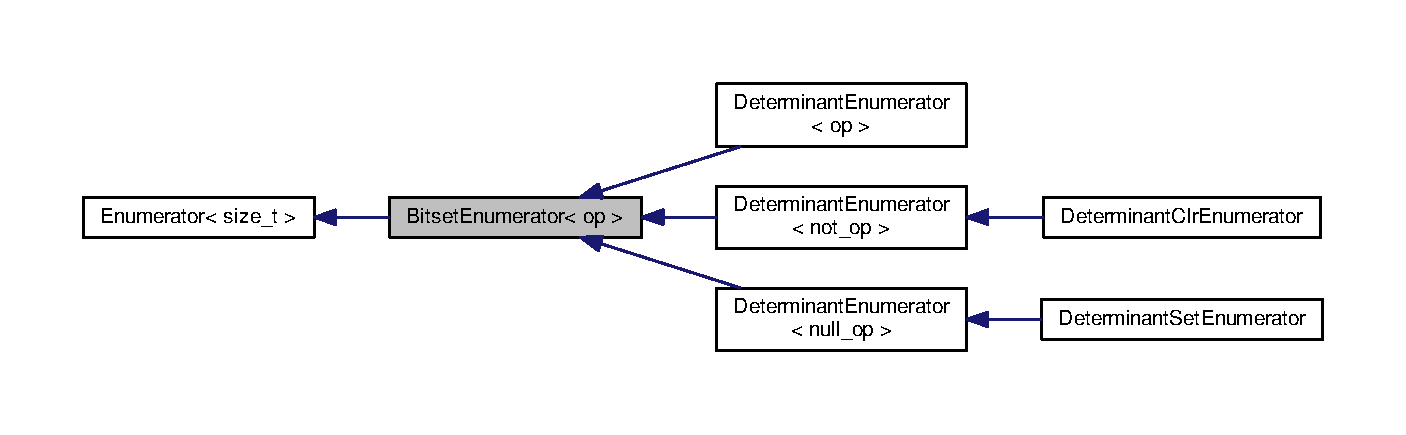
\includegraphics[width=350pt]{classBitsetEnumerator__inherit__graph}
\end{center}
\end{figure}


Collaboration diagram for Bitset\+Enumerator$<$ op $>$\+:\nopagebreak
\begin{figure}[H]
\begin{center}
\leavevmode
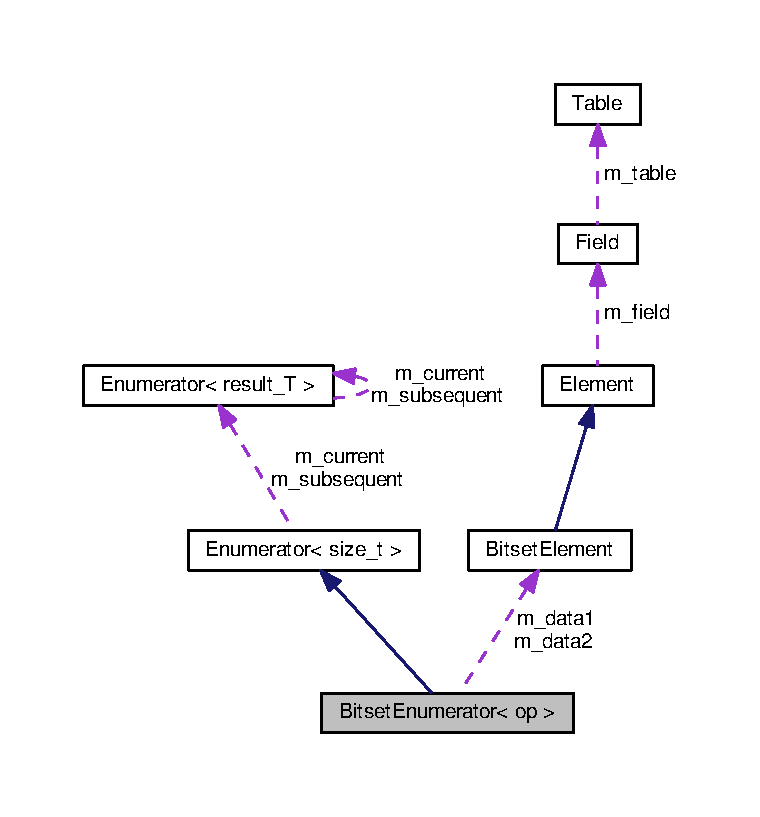
\includegraphics[width=350pt]{classBitsetEnumerator__coll__graph}
\end{center}
\end{figure}
\doxysubsection*{Public Member Functions}
\begin{DoxyCompactItemize}
\item 
\mbox{\Hypertarget{classBitsetEnumerator_a4c5297e92189eb2db688d5ae95aa074c}\label{classBitsetEnumerator_a4c5297e92189eb2db688d5ae95aa074c}} 
{\bfseries Bitset\+Enumerator} (const \mbox{\hyperlink{classBitsetElement}{Bitset\+Element}} \&data1, const \mbox{\hyperlink{classBitsetElement}{Bitset\+Element}} \&data2, \mbox{\hyperlink{classEnumerator}{Enumerator}} $\ast$subsequent=nullptr, size\+\_\+t offset=0)
\item 
\mbox{\Hypertarget{classBitsetEnumerator_a4b39060663550c127c5aa238865c94c4}\label{classBitsetEnumerator_a4b39060663550c127c5aa238865c94c4}} 
bool {\bfseries next\+\_\+element} (size\+\_\+t \&result) override
\item 
\mbox{\Hypertarget{classBitsetEnumerator_a0784fb3256950e358557776ed71abf05}\label{classBitsetEnumerator_a0784fb3256950e358557776ed71abf05}} 
defs\+::data\+\_\+t {\bfseries get\+\_\+work} (const size\+\_\+t \&idata) const
\end{DoxyCompactItemize}
\doxysubsection*{Protected Attributes}
\begin{DoxyCompactItemize}
\item 
\mbox{\Hypertarget{classBitsetEnumerator_a7a9c33fce104b03ad93e982e84043de7}\label{classBitsetEnumerator_a7a9c33fce104b03ad93e982e84043de7}} 
const \mbox{\hyperlink{classBitsetElement}{Bitset\+Element}} \& {\bfseries m\+\_\+data1}
\item 
\mbox{\Hypertarget{classBitsetEnumerator_aae1ee3784204f62f1759bf681ee28a4f}\label{classBitsetEnumerator_aae1ee3784204f62f1759bf681ee28a4f}} 
const \mbox{\hyperlink{classBitsetElement}{Bitset\+Element}} \& {\bfseries m\+\_\+data2}
\item 
\mbox{\Hypertarget{classBitsetEnumerator_a5b51d281c1d7e85a4f102a9ed85528ae}\label{classBitsetEnumerator_a5b51d281c1d7e85a4f102a9ed85528ae}} 
size\+\_\+t {\bfseries m\+\_\+offset}
\item 
\mbox{\Hypertarget{classBitsetEnumerator_a45e95ec5fc9a2d27c63023947d501092}\label{classBitsetEnumerator_a45e95ec5fc9a2d27c63023947d501092}} 
size\+\_\+t {\bfseries m\+\_\+idata} = $\sim$0ul
\item 
\mbox{\Hypertarget{classBitsetEnumerator_a3b3e4114e11171be5bc918362ecda275}\label{classBitsetEnumerator_a3b3e4114e11171be5bc918362ecda275}} 
defs\+::data\+\_\+t {\bfseries m\+\_\+work} = 0ul
\end{DoxyCompactItemize}
\doxysubsection*{Additional Inherited Members}


The documentation for this class was generated from the following file\+:\begin{DoxyCompactItemize}
\item 
/home/teamcity/\+Team\+City/build\+Agent/work/5343cdffda4690e5/src/core/enumerator/Bitset\+Enumerator.\+h\end{DoxyCompactItemize}

\hypertarget{classBitsetField}{}\section{Bitset\+Field Class Reference}
\label{classBitsetField}\index{Bitset\+Field@{Bitset\+Field}}


Inheritance diagram for Bitset\+Field\+:
\nopagebreak
\begin{figure}[H]
\begin{center}
\leavevmode
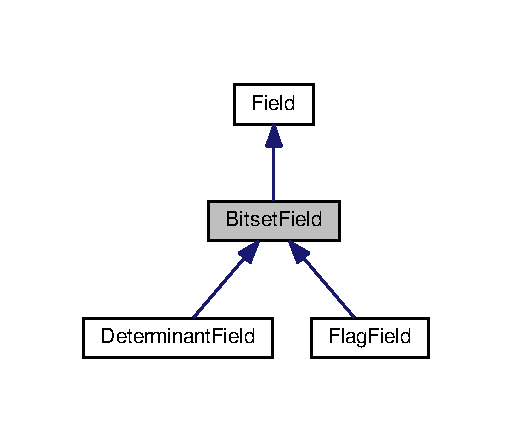
\includegraphics[width=246pt]{classBitsetField__inherit__graph}
\end{center}
\end{figure}


Collaboration diagram for Bitset\+Field\+:
\nopagebreak
\begin{figure}[H]
\begin{center}
\leavevmode
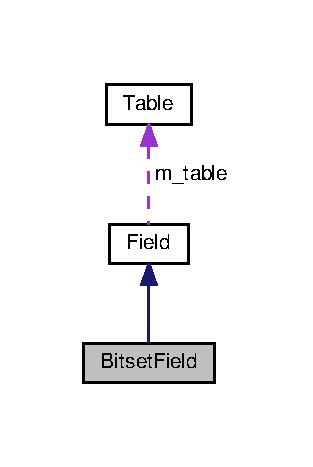
\includegraphics[width=150pt]{classBitsetField__coll__graph}
\end{center}
\end{figure}
\subsection*{Public Member Functions}
\begin{DoxyCompactItemize}
\item 
{\bfseries Bitset\+Field} (\hyperlink{classTable}{Table} $\ast$table, size\+\_\+t nelement, size\+\_\+t nbit, const std\+::string \&description=\char`\"{}\char`\"{})\hypertarget{classBitsetField_a63cb4af7c310f66d13eaa3e406083bab}{}\label{classBitsetField_a63cb4af7c310f66d13eaa3e406083bab}

\item 
size\+\_\+t {\bfseries nbit} () const override\hypertarget{classBitsetField_a8e791b6dcc0a47a33eb8f6f0f2a242c9}{}\label{classBitsetField_a8e791b6dcc0a47a33eb8f6f0f2a242c9}

\item 
\hyperlink{classBitsetElement}{Bitset\+Element} {\bfseries operator()} (const size\+\_\+t \&irow, const size\+\_\+t \&isegment=0, const size\+\_\+t \&ielement=0)\hypertarget{classBitsetField_aafbbb0286abfdfae29e12a74bc9d17a7}{}\label{classBitsetField_aafbbb0286abfdfae29e12a74bc9d17a7}

\item 
std\+::string {\bfseries to\+\_\+string} (size\+\_\+t irow, size\+\_\+t isegment, size\+\_\+t ielement) override\hypertarget{classBitsetField_a74210dfe93e12911b41fa22d328555a0}{}\label{classBitsetField_a74210dfe93e12911b41fa22d328555a0}

\end{DoxyCompactItemize}
\subsection*{Static Public Member Functions}
\begin{DoxyCompactItemize}
\item 
static defs\+::pair {\bfseries rectify\+\_\+offset} (const defs\+::pair \&pair)\hypertarget{classBitsetField_a2ed3cd55b88444348643ae5fdd6bb2b4}{}\label{classBitsetField_a2ed3cd55b88444348643ae5fdd6bb2b4}

\end{DoxyCompactItemize}
\subsection*{Protected Member Functions}
\begin{DoxyCompactItemize}
\item 
virtual void {\bfseries update\+\_\+nbit} (size\+\_\+t nbit)\hypertarget{classBitsetField_ad8fadd64db86e4df4566d07633a0f2d0}{}\label{classBitsetField_ad8fadd64db86e4df4566d07633a0f2d0}

\item 
void {\bfseries increment\+\_\+nbit} (size\+\_\+t nbit)\hypertarget{classBitsetField_a42665f70a291b36fbd68f119094b1768}{}\label{classBitsetField_a42665f70a291b36fbd68f119094b1768}

\end{DoxyCompactItemize}
\subsection*{Protected Attributes}
\begin{DoxyCompactItemize}
\item 
size\+\_\+t {\bfseries m\+\_\+nbit}\hypertarget{classBitsetField_aa93dab557a478225c412d7aa0683396b}{}\label{classBitsetField_aa93dab557a478225c412d7aa0683396b}

\end{DoxyCompactItemize}


The documentation for this class was generated from the following files\+:\begin{DoxyCompactItemize}
\item 
/home/teamcity/\+Team\+City/build\+Agent/work/5343cdffda4690e5/src/core/table/Bitset\+Field.\+h\item 
/home/teamcity/\+Team\+City/build\+Agent/work/5343cdffda4690e5/src/core/table/Bitset\+Field.\+cpp\end{DoxyCompactItemize}

\hypertarget{classBitsetSetEnumerator}{}\doxysection{Bitset\+Set\+Enumerator Class Reference}
\label{classBitsetSetEnumerator}\index{BitsetSetEnumerator@{BitsetSetEnumerator}}


Inheritance diagram for Bitset\+Set\+Enumerator\+:\nopagebreak
\begin{figure}[H]
\begin{center}
\leavevmode
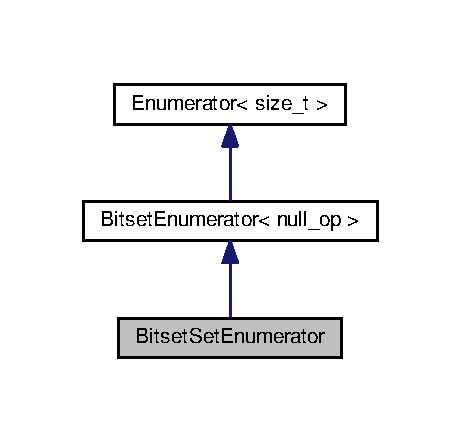
\includegraphics[width=221pt]{classBitsetSetEnumerator__inherit__graph}
\end{center}
\end{figure}


Collaboration diagram for Bitset\+Set\+Enumerator\+:\nopagebreak
\begin{figure}[H]
\begin{center}
\leavevmode
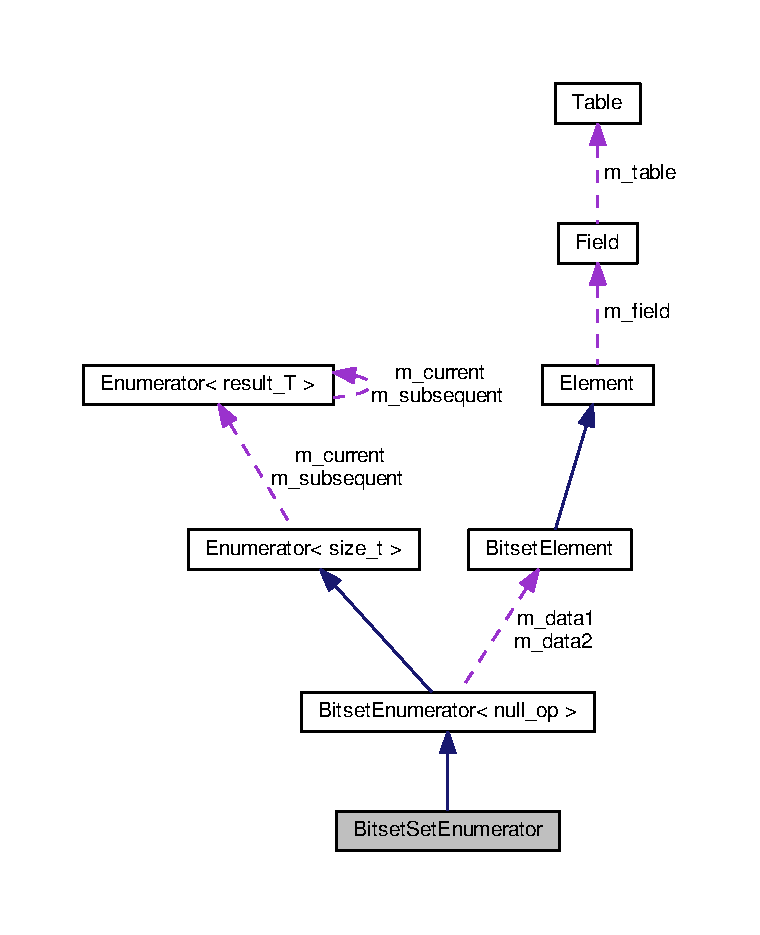
\includegraphics[width=350pt]{classBitsetSetEnumerator__coll__graph}
\end{center}
\end{figure}
\doxysubsection*{Public Member Functions}
\begin{DoxyCompactItemize}
\item 
\mbox{\Hypertarget{classBitsetSetEnumerator_a0edfcef06f94f81e2faf8ad9eca0c791}\label{classBitsetSetEnumerator_a0edfcef06f94f81e2faf8ad9eca0c791}} 
{\bfseries Bitset\+Set\+Enumerator} (const \mbox{\hyperlink{classBitsetElement}{Bitset\+Element}} \&data1, \mbox{\hyperlink{classEnumerator}{Enumerator}}$<$ size\+\_\+t $>$ $\ast$subsequent=nullptr, size\+\_\+t offset=0)
\end{DoxyCompactItemize}
\doxysubsection*{Additional Inherited Members}


The documentation for this class was generated from the following file\+:\begin{DoxyCompactItemize}
\item 
/home/teamcity/\+Team\+City/build\+Agent/work/5343cdffda4690e5/src/core/enumerator/Bitset\+Enumerator.\+h\end{DoxyCompactItemize}

\hypertarget{classCombinationEnumerator}{}\doxysection{Combination\+Enumerator Class Reference}
\label{classCombinationEnumerator}\index{CombinationEnumerator@{CombinationEnumerator}}


Inheritance diagram for Combination\+Enumerator\+:\nopagebreak
\begin{figure}[H]
\begin{center}
\leavevmode
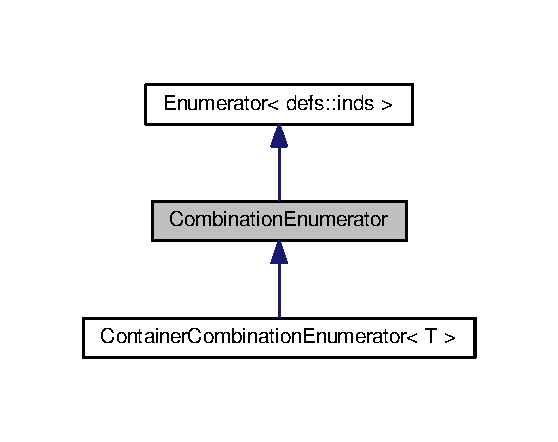
\includegraphics[width=268pt]{classCombinationEnumerator__inherit__graph}
\end{center}
\end{figure}


Collaboration diagram for Combination\+Enumerator\+:\nopagebreak
\begin{figure}[H]
\begin{center}
\leavevmode
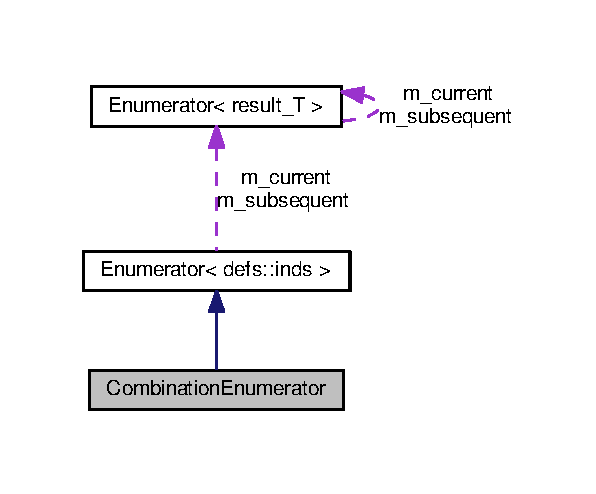
\includegraphics[width=286pt]{classCombinationEnumerator__coll__graph}
\end{center}
\end{figure}
\doxysubsection*{Public Member Functions}
\begin{DoxyCompactItemize}
\item 
\mbox{\Hypertarget{classCombinationEnumerator_a26b255c3e1743191189c68cff3a93120}\label{classCombinationEnumerator_a26b255c3e1743191189c68cff3a93120}} 
{\bfseries Combination\+Enumerator} (size\+\_\+t n, size\+\_\+t r, \mbox{\hyperlink{classEnumerator}{Enumerator}} $\ast$subsequent=nullptr)
\item 
\mbox{\Hypertarget{classCombinationEnumerator_a7e9a1848cae9ef46a65883b47f76d994}\label{classCombinationEnumerator_a7e9a1848cae9ef46a65883b47f76d994}} 
virtual bool {\bfseries next\+\_\+element} (defs\+::inds \&result)
\item 
\mbox{\Hypertarget{classCombinationEnumerator_aec8be6907ffc568e9d665184630f0d5e}\label{classCombinationEnumerator_aec8be6907ffc568e9d665184630f0d5e}} 
defs\+::inds {\bfseries default\+\_\+result} () override
\end{DoxyCompactItemize}
\doxysubsection*{Additional Inherited Members}


The documentation for this class was generated from the following files\+:\begin{DoxyCompactItemize}
\item 
/home/teamcity/\+Team\+City/build\+Agent/work/5343cdffda4690e5/src/core/enumerator/Combination\+Enumerator.\+h\item 
/home/teamcity/\+Team\+City/build\+Agent/work/5343cdffda4690e5/src/core/enumerator/Combination\+Enumerator.\+cpp\end{DoxyCompactItemize}

\hypertarget{structconsts_1_1component__t}{}\doxysection{consts\+::component\+\_\+t$<$ T $>$ Struct Template Reference}
\label{structconsts_1_1component__t}\index{consts::component\_t$<$ T $>$@{consts::component\_t$<$ T $>$}}
\doxysubsection*{Public Types}
\begin{DoxyCompactItemize}
\item 
\mbox{\Hypertarget{structconsts_1_1component__t_a3c8d59aa909fe6a8271b795ed8d34f3e}\label{structconsts_1_1component__t_a3c8d59aa909fe6a8271b795ed8d34f3e}} 
typedef T {\bfseries type}
\end{DoxyCompactItemize}


The documentation for this struct was generated from the following file\+:\begin{DoxyCompactItemize}
\item 
/home/teamcity/\+Team\+City/build\+Agent/work/5343cdffda4690e5/src/core/util/consts.\+h\end{DoxyCompactItemize}

\hypertarget{structconsts_1_1component__t_3_01const_01std_1_1complex_3_01T_01_4_01_6_01_4}{}\doxysection{consts\+::component\+\_\+t$<$ const std\+::complex$<$ T $>$ \& $>$ Struct Template Reference}
\label{structconsts_1_1component__t_3_01const_01std_1_1complex_3_01T_01_4_01_6_01_4}\index{consts::component\_t$<$ const std::complex$<$ T $>$ \& $>$@{consts::component\_t$<$ const std::complex$<$ T $>$ \& $>$}}
\doxysubsection*{Public Types}
\begin{DoxyCompactItemize}
\item 
\mbox{\Hypertarget{structconsts_1_1component__t_3_01const_01std_1_1complex_3_01T_01_4_01_6_01_4_a9cc3483e66e52b0c195e16b93a7548c3}\label{structconsts_1_1component__t_3_01const_01std_1_1complex_3_01T_01_4_01_6_01_4_a9cc3483e66e52b0c195e16b93a7548c3}} 
typedef T {\bfseries type}
\end{DoxyCompactItemize}


The documentation for this struct was generated from the following file\+:\begin{DoxyCompactItemize}
\item 
/home/teamcity/\+Team\+City/build\+Agent/work/5343cdffda4690e5/src/core/util/consts.\+h\end{DoxyCompactItemize}

\hypertarget{structconsts_1_1component__t_3_01std_1_1complex_3_01T_01_4_01_4}{}\doxysection{consts\+::component\+\_\+t$<$ std\+::complex$<$ T $>$ $>$ Struct Template Reference}
\label{structconsts_1_1component__t_3_01std_1_1complex_3_01T_01_4_01_4}\index{consts::component\_t$<$ std::complex$<$ T $>$ $>$@{consts::component\_t$<$ std::complex$<$ T $>$ $>$}}
\doxysubsection*{Public Types}
\begin{DoxyCompactItemize}
\item 
\mbox{\Hypertarget{structconsts_1_1component__t_3_01std_1_1complex_3_01T_01_4_01_4_acd8a85832d750cfcabf03a56fecdff9f}\label{structconsts_1_1component__t_3_01std_1_1complex_3_01T_01_4_01_4_acd8a85832d750cfcabf03a56fecdff9f}} 
typedef T {\bfseries type}
\end{DoxyCompactItemize}


The documentation for this struct was generated from the following file\+:\begin{DoxyCompactItemize}
\item 
/home/teamcity/\+Team\+City/build\+Agent/work/5343cdffda4690e5/src/core/util/consts.\+h\end{DoxyCompactItemize}

\hypertarget{classConnection}{}\section{Connection Class Reference}
\label{classConnection}\index{Connection@{Connection}}


Inheritance diagram for Connection\+:
% FIG 0
\subsection*{Public Member Functions}
\begin{DoxyCompactItemize}
\item 
{\bfseries Connection} (const \hyperlink{classField}{Field} $\ast$field)\hypertarget{classConnection_af4ce8512ec2e108246299a672a8c6631}{}\label{classConnection_af4ce8512ec2e108246299a672a8c6631}

\item 
{\bfseries Connection} (const \hyperlink{classDeterminantElement}{Determinant\+Element} \&ket, const \hyperlink{classDeterminantElement}{Determinant\+Element} \&bra)\hypertarget{classConnection_a0b96cb58be47c490e4be42a13aae4830}{}\label{classConnection_a0b96cb58be47c490e4be42a13aae4830}

\item 
{\bfseries Connection} (const \hyperlink{classDeterminantElement}{Determinant\+Element} \&ket)\hypertarget{classConnection_ab9d08b55aa2848e5fb6243b543c7c1bb}{}\label{classConnection_ab9d08b55aa2848e5fb6243b543c7c1bb}

\item 
const defs\+::det\+\_\+work \& {\bfseries ann} () const \hypertarget{classConnection_a6be30329b0ea0260472704342cbd435c}{}\label{classConnection_a6be30329b0ea0260472704342cbd435c}

\item 
const size\+\_\+t \& {\bfseries ann} (const size\+\_\+t \&i) const \hypertarget{classConnection_ad672469fe1158702fabc342bb34fc31b}{}\label{classConnection_ad672469fe1158702fabc342bb34fc31b}

\item 
const size\+\_\+t \& {\bfseries nann} () const \hypertarget{classConnection_a3e3347717f29609432141b7eedf750ed}{}\label{classConnection_a3e3347717f29609432141b7eedf750ed}

\item 
const defs\+::det\+\_\+work \& {\bfseries cre} () const \hypertarget{classConnection_a7ac096bbf08c67fc11f7cd8be4e25e47}{}\label{classConnection_a7ac096bbf08c67fc11f7cd8be4e25e47}

\item 
const size\+\_\+t \& {\bfseries cre} (const size\+\_\+t \&i) const \hypertarget{classConnection_a4b466c63cf29f3c8f70b90e4824f2c49}{}\label{classConnection_a4b466c63cf29f3c8f70b90e4824f2c49}

\item 
const size\+\_\+t \& {\bfseries ncre} () const \hypertarget{classConnection_aa6f76ca038d3183e4fdf5f94e47e1a19}{}\label{classConnection_aa6f76ca038d3183e4fdf5f94e47e1a19}

\item 
virtual void {\bfseries connect} (const \hyperlink{classDeterminantElement}{Determinant\+Element} \&ket, const \hyperlink{classDeterminantElement}{Determinant\+Element} \&bra)\hypertarget{classConnection_a0c843525d4e2934fdaf10e9fad2bd50a}{}\label{classConnection_a0c843525d4e2934fdaf10e9fad2bd50a}

\item 
virtual void {\bfseries apply} (const \hyperlink{classDeterminantElement}{Determinant\+Element} \&ket, \hyperlink{classDeterminantElement}{Determinant\+Element} \&bra)\hypertarget{classConnection_a81b694174d09ef90256f705410b651e7}{}\label{classConnection_a81b694174d09ef90256f705410b651e7}

\item 
void {\bfseries zero} ()\hypertarget{classConnection_a07e46eda12da6ff7e5cfb66b00f716ac}{}\label{classConnection_a07e46eda12da6ff7e5cfb66b00f716ac}

\item 
void {\bfseries add\+\_\+cre} (const size\+\_\+t \&i)\hypertarget{classConnection_af617fea5e5082c941470eae7a795367c}{}\label{classConnection_af617fea5e5082c941470eae7a795367c}

\item 
void {\bfseries add\+\_\+ann} (const size\+\_\+t \&i)\hypertarget{classConnection_ad967f8812d0598ba228ef16b2f7436a5}{}\label{classConnection_ad967f8812d0598ba228ef16b2f7436a5}

\item 
void {\bfseries add} (const size\+\_\+t \&ann, const size\+\_\+t \&cre)\hypertarget{classConnection_af167b1fd395bceea3540d720437adf55}{}\label{classConnection_af167b1fd395bceea3540d720437adf55}

\item 
void {\bfseries add} (const size\+\_\+t \&ann1, const size\+\_\+t \&ann2, const size\+\_\+t \&cre1, const size\+\_\+t \&cre2)\hypertarget{classConnection_a4a7ab2893fb8b3a21162a055c3065c3c}{}\label{classConnection_a4a7ab2893fb8b3a21162a055c3065c3c}

\item 
void {\bfseries sort} ()\hypertarget{classConnection_ae50daf05c5a97ea366f26cbd7e2d0fe7}{}\label{classConnection_ae50daf05c5a97ea366f26cbd7e2d0fe7}

\item 
const size\+\_\+t \& {\bfseries nexcit} () const \hypertarget{classConnection_a7e83ced8023d813160513729b9216ede}{}\label{classConnection_a7e83ced8023d813160513729b9216ede}

\end{DoxyCompactItemize}
\subsection*{Protected Attributes}
\begin{DoxyCompactItemize}
\item 
const size\+\_\+t {\bfseries m\+\_\+nbit}\hypertarget{classConnection_a8aadc0ee3e3e3fe998c5f4815f04e2e8}{}\label{classConnection_a8aadc0ee3e3e3fe998c5f4815f04e2e8}

\item 
defs\+::det\+\_\+work {\bfseries m\+\_\+ann} \{\}\hypertarget{classConnection_aab1226dd30dcdd41602974626a2a1e71}{}\label{classConnection_aab1226dd30dcdd41602974626a2a1e71}

\item 
defs\+::det\+\_\+work {\bfseries m\+\_\+cre} \{\}\hypertarget{classConnection_a6885ccdb80c52b6042974655b2188340}{}\label{classConnection_a6885ccdb80c52b6042974655b2188340}

\item 
size\+\_\+t {\bfseries m\+\_\+nann}\hypertarget{classConnection_a3335fdc82d07554572094f3003aa3076}{}\label{classConnection_a3335fdc82d07554572094f3003aa3076}

\item 
size\+\_\+t {\bfseries m\+\_\+ncre}\hypertarget{classConnection_a705e6a0307c83e213a0587804a5c2c91}{}\label{classConnection_a705e6a0307c83e213a0587804a5c2c91}

\end{DoxyCompactItemize}


The documentation for this class was generated from the following files\+:\begin{DoxyCompactItemize}
\item 
/home/teamcity/\+Team\+City/build\+Agent/work/5343cdffda4690e5/src/core/fermion/Connection.\+h\item 
/home/teamcity/\+Team\+City/build\+Agent/work/5343cdffda4690e5/src/core/fermion/Connection.\+cpp\end{DoxyCompactItemize}

\hypertarget{classHamiltonian_1_1ConnectionList}{}\section{Hamiltonian\+:\+:Connection\+List Class Reference}
\label{classHamiltonian_1_1ConnectionList}\index{Hamiltonian\+::\+Connection\+List@{Hamiltonian\+::\+Connection\+List}}


Inheritance diagram for Hamiltonian\+:\+:Connection\+List\+:
\nopagebreak
\begin{figure}[H]
\begin{center}
\leavevmode
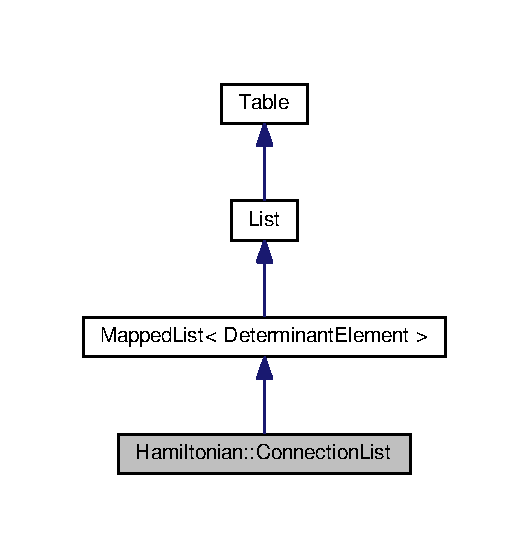
\includegraphics[width=254pt]{classHamiltonian_1_1ConnectionList__inherit__graph}
\end{center}
\end{figure}


Collaboration diagram for Hamiltonian\+:\+:Connection\+List\+:
\nopagebreak
\begin{figure}[H]
\begin{center}
\leavevmode
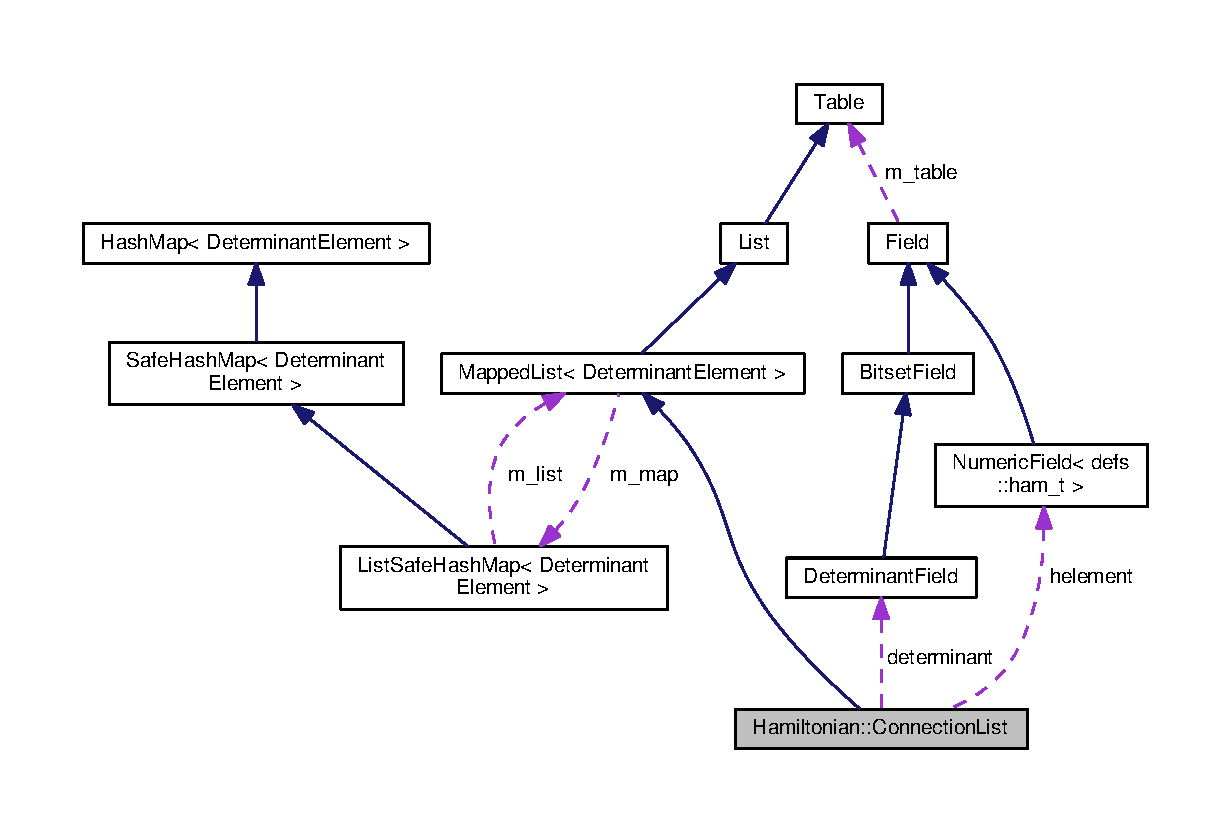
\includegraphics[width=350pt]{classHamiltonian_1_1ConnectionList__coll__graph}
\end{center}
\end{figure}
\subsection*{Public Member Functions}
\begin{DoxyCompactItemize}
\item 
{\bfseries Connection\+List} (size\+\_\+t nsite, size\+\_\+t nbucket)\hypertarget{classHamiltonian_1_1ConnectionList_a8696d497d05710f3bfb3eff5cdaea200}{}\label{classHamiltonian_1_1ConnectionList_a8696d497d05710f3bfb3eff5cdaea200}

\end{DoxyCompactItemize}
\subsection*{Public Attributes}
\begin{DoxyCompactItemize}
\item 
\hyperlink{classDeterminantField}{Determinant\+Field} {\bfseries determinant}\hypertarget{classHamiltonian_1_1ConnectionList_a6b8f99fc32cdc563a8863dc8b81c3e87}{}\label{classHamiltonian_1_1ConnectionList_a6b8f99fc32cdc563a8863dc8b81c3e87}

\item 
\hyperlink{classNumericField}{Numeric\+Field}$<$ defs\+::ham\+\_\+t $>$ {\bfseries helement}\hypertarget{classHamiltonian_1_1ConnectionList_a2e15f602fe21f932f3c1980cb7580d0e}{}\label{classHamiltonian_1_1ConnectionList_a2e15f602fe21f932f3c1980cb7580d0e}

\end{DoxyCompactItemize}
\subsection*{Additional Inherited Members}


The documentation for this class was generated from the following file\+:\begin{DoxyCompactItemize}
\item 
/home/teamcity/\+Team\+City/build\+Agent/work/5343cdffda4690e5/src/core/hamiltonian/Hamiltonian.\+h\end{DoxyCompactItemize}

\hypertarget{classContainerCombinationEnumerator}{}\section{Container\+Combination\+Enumerator$<$ T $>$ Class Template Reference}
\label{classContainerCombinationEnumerator}\index{Container\+Combination\+Enumerator$<$ T $>$@{Container\+Combination\+Enumerator$<$ T $>$}}


Inheritance diagram for Container\+Combination\+Enumerator$<$ T $>$\+:
% FIG 0


Collaboration diagram for Container\+Combination\+Enumerator$<$ T $>$\+:
% FIG 1
\subsection*{Public Member Functions}
\begin{DoxyCompactItemize}
\item 
{\bfseries Container\+Combination\+Enumerator} (const T \&container, size\+\_\+t n, size\+\_\+t r, \hyperlink{classEnumerator}{Enumerator} $\ast$subsequent=nullptr)\hypertarget{classContainerCombinationEnumerator_ad3766343b798d5e95a94aa90f05fccfe}{}\label{classContainerCombinationEnumerator_ad3766343b798d5e95a94aa90f05fccfe}

\item 
{\bfseries Container\+Combination\+Enumerator} (const T \&container, size\+\_\+t r, \hyperlink{classEnumerator}{Enumerator} $\ast$subsequent=nullptr)\hypertarget{classContainerCombinationEnumerator_aa0f06fe46f5a701b0c47aa4ca5e7531e}{}\label{classContainerCombinationEnumerator_aa0f06fe46f5a701b0c47aa4ca5e7531e}

\item 
bool {\bfseries next\+\_\+element} (defs\+::inds \&result) override\hypertarget{classContainerCombinationEnumerator_a5ae4cc19cd270528b56f5f9f2b9d5fd5}{}\label{classContainerCombinationEnumerator_a5ae4cc19cd270528b56f5f9f2b9d5fd5}

\end{DoxyCompactItemize}
\subsection*{Additional Inherited Members}


The documentation for this class was generated from the following file\+:\begin{DoxyCompactItemize}
\item 
/home/teamcity/\+Team\+City/build\+Agent/work/5343cdffda4690e5/src/core/enumerator/Container\+Combination\+Enumerator.\+h\end{DoxyCompactItemize}

\hypertarget{classDeterminantElement_1_1DatawordEnumerator}{}\section{Determinant\+Element\+:\+:Dataword\+Enumerator Class Reference}
\label{classDeterminantElement_1_1DatawordEnumerator}\index{Determinant\+Element\+::\+Dataword\+Enumerator@{Determinant\+Element\+::\+Dataword\+Enumerator}}


Inheritance diagram for Determinant\+Element\+:\+:Dataword\+Enumerator\+:
\nopagebreak
\begin{figure}[H]
\begin{center}
\leavevmode
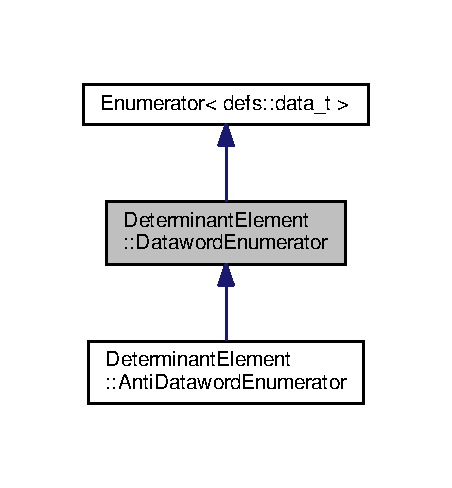
\includegraphics[width=217pt]{classDeterminantElement_1_1DatawordEnumerator__inherit__graph}
\end{center}
\end{figure}


Collaboration diagram for Determinant\+Element\+:\+:Dataword\+Enumerator\+:
\nopagebreak
\begin{figure}[H]
\begin{center}
\leavevmode
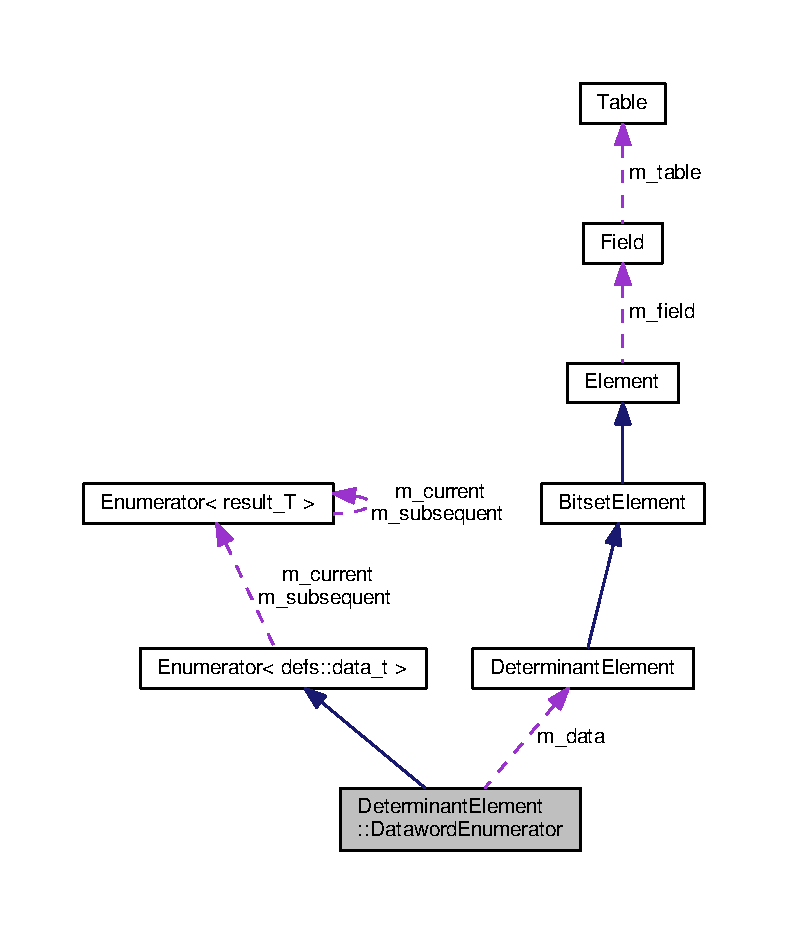
\includegraphics[width=350pt]{classDeterminantElement_1_1DatawordEnumerator__coll__graph}
\end{center}
\end{figure}
\subsection*{Public Member Functions}
\begin{DoxyCompactItemize}
\item 
{\bfseries Dataword\+Enumerator} (const \hyperlink{classDeterminantElement}{Determinant\+Element} \&data)\hypertarget{classDeterminantElement_1_1DatawordEnumerator_a17237d87203d5ad9874dd2326858f061}{}\label{classDeterminantElement_1_1DatawordEnumerator_a17237d87203d5ad9874dd2326858f061}

\end{DoxyCompactItemize}
\subsection*{Protected Member Functions}
\begin{DoxyCompactItemize}
\item 
virtual size\+\_\+t {\bfseries get\+\_\+dataword} (const size\+\_\+t \&idataword)\hypertarget{classDeterminantElement_1_1DatawordEnumerator_ae38acfbe1b6c240511f2c683b80abecb}{}\label{classDeterminantElement_1_1DatawordEnumerator_ae38acfbe1b6c240511f2c683b80abecb}

\item 
virtual size\+\_\+t {\bfseries get\+\_\+dataword} (const size\+\_\+t \&idataword, const size\+\_\+t \&nbit)\hypertarget{classDeterminantElement_1_1DatawordEnumerator_a12c2391ace451e06c881897c5b4079ac}{}\label{classDeterminantElement_1_1DatawordEnumerator_a12c2391ace451e06c881897c5b4079ac}

\item 
bool {\bfseries next\+\_\+element} (defs\+::data\+\_\+t \&result) override\hypertarget{classDeterminantElement_1_1DatawordEnumerator_a8d7af22fcc9e1b15a2989e48f2fb0988}{}\label{classDeterminantElement_1_1DatawordEnumerator_a8d7af22fcc9e1b15a2989e48f2fb0988}

\end{DoxyCompactItemize}
\subsection*{Protected Attributes}
\begin{DoxyCompactItemize}
\item 
size\+\_\+t {\bfseries m\+\_\+idataword} = 0ul\hypertarget{classDeterminantElement_1_1DatawordEnumerator_a1b22f498dcfa87d06d556559879e6b50}{}\label{classDeterminantElement_1_1DatawordEnumerator_a1b22f498dcfa87d06d556559879e6b50}

\item 
const \hyperlink{classDeterminantElement}{Determinant\+Element} \& {\bfseries m\+\_\+data}\hypertarget{classDeterminantElement_1_1DatawordEnumerator_ab4dcfbb2b8b76ccdb76389e39139120d}{}\label{classDeterminantElement_1_1DatawordEnumerator_ab4dcfbb2b8b76ccdb76389e39139120d}

\end{DoxyCompactItemize}


The documentation for this class was generated from the following file\+:\begin{DoxyCompactItemize}
\item 
/home/teamcity/\+Team\+City/build\+Agent/work/5343cdffda4690e5/src/core/table/Determinant\+Field.\+h\end{DoxyCompactItemize}

\hypertarget{structDecodedDeterminant}{}\doxysection{Decoded\+Determinant Struct Reference}
\label{structDecodedDeterminant}\index{DecodedDeterminant@{DecodedDeterminant}}


Inheritance diagram for Decoded\+Determinant\+:\nopagebreak
\begin{figure}[H]
\begin{center}
\leavevmode
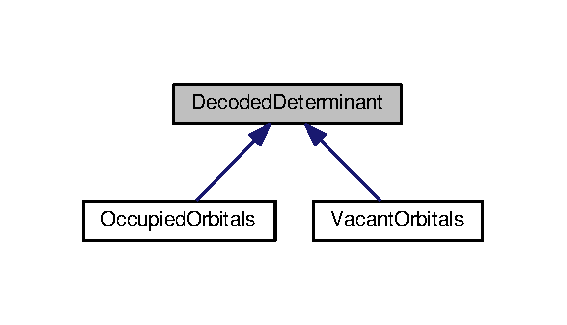
\includegraphics[width=272pt]{structDecodedDeterminant__inherit__graph}
\end{center}
\end{figure}
\doxysubsection*{Public Member Functions}
\begin{DoxyCompactItemize}
\item 
\mbox{\Hypertarget{structDecodedDeterminant_a0735455c5d917595573d4710dd8fe61a}\label{structDecodedDeterminant_a0735455c5d917595573d4710dd8fe61a}} 
{\bfseries Decoded\+Determinant} (const \mbox{\hyperlink{classField}{Field}} $\ast$field)
\item 
\mbox{\Hypertarget{structDecodedDeterminant_a694c656a8d47a8637fff4bd23f3bc543}\label{structDecodedDeterminant_a694c656a8d47a8637fff4bd23f3bc543}} 
{\bfseries Decoded\+Determinant} (const \mbox{\hyperlink{classDeterminantElement}{Determinant\+Element}} \&det\+\_\+elem)
\item 
\mbox{\Hypertarget{structDecodedDeterminant_a9d957e501d01a230a41521595377f66d}\label{structDecodedDeterminant_a9d957e501d01a230a41521595377f66d}} 
virtual void {\bfseries update} (const \mbox{\hyperlink{classDeterminantElement}{Determinant\+Element}} \&det\+\_\+elem)=0
\end{DoxyCompactItemize}
\doxysubsection*{Public Attributes}
\begin{DoxyCompactItemize}
\item 
\mbox{\Hypertarget{structDecodedDeterminant_aa085943321206f6933ea1b39f63538b8}\label{structDecodedDeterminant_aa085943321206f6933ea1b39f63538b8}} 
const size\+\_\+t {\bfseries m\+\_\+nbit}
\item 
\mbox{\Hypertarget{structDecodedDeterminant_a28791ac6bd8b5af4e487bee525200036}\label{structDecodedDeterminant_a28791ac6bd8b5af4e487bee525200036}} 
const size\+\_\+t {\bfseries m\+\_\+element\+\_\+dsize}
\item 
\mbox{\Hypertarget{structDecodedDeterminant_a54abd377e297c333dd4bdd6675badee5}\label{structDecodedDeterminant_a54abd377e297c333dd4bdd6675badee5}} 
defs\+::det\+\_\+work {\bfseries m\+\_\+inds} \{\}
\item 
\mbox{\Hypertarget{structDecodedDeterminant_a002d04b059a903938f644dea5c7d8648}\label{structDecodedDeterminant_a002d04b059a903938f644dea5c7d8648}} 
size\+\_\+t {\bfseries m\+\_\+nind} = 0ul
\end{DoxyCompactItemize}


The documentation for this struct was generated from the following file\+:\begin{DoxyCompactItemize}
\item 
/home/teamcity/\+Team\+City/build\+Agent/work/5343cdffda4690e5/src/core/fermion/Decoded\+Determinant.\+h\end{DoxyCompactItemize}

\hypertarget{classDenseHamiltonian}{}\section{Dense\+Hamiltonian Class Reference}
\label{classDenseHamiltonian}\index{Dense\+Hamiltonian@{Dense\+Hamiltonian}}


Inheritance diagram for Dense\+Hamiltonian\+:\nopagebreak
\begin{figure}[H]
\begin{center}
\leavevmode
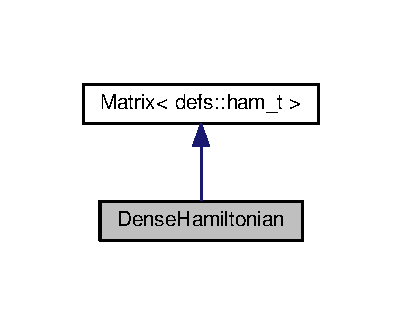
\includegraphics[width=193pt]{classDenseHamiltonian__inherit__graph}
\end{center}
\end{figure}


Collaboration diagram for Dense\+Hamiltonian\+:\nopagebreak
\begin{figure}[H]
\begin{center}
\leavevmode
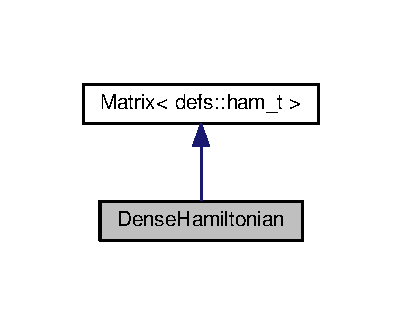
\includegraphics[width=193pt]{classDenseHamiltonian__coll__graph}
\end{center}
\end{figure}
\subsection*{Public Member Functions}
\begin{DoxyCompactItemize}
\item 
{\bfseries Dense\+Hamiltonian} (const \hyperlink{classHamiltonian}{Hamiltonian} \&source)\hypertarget{classDenseHamiltonian_ad171bef2d0b359ea8f93a56b1932272d}{}\label{classDenseHamiltonian_ad171bef2d0b359ea8f93a56b1932272d}

\end{DoxyCompactItemize}
\subsection*{Additional Inherited Members}


The documentation for this class was generated from the following files\+:\begin{DoxyCompactItemize}
\item 
/home/teamcity/\+Team\+City/build\+Agent/work/5343cdffda4690e5/src/core/linalg/Dense\+Hamiltonian.\+h\item 
/home/teamcity/\+Team\+City/build\+Agent/work/5343cdffda4690e5/src/core/linalg/Dense\+Hamiltonian.\+cpp\end{DoxyCompactItemize}

\hypertarget{classDeterminant}{}\section{Determinant Class Reference}
\label{classDeterminant}\index{Determinant@{Determinant}}


Inheritance diagram for Determinant\+:
\nopagebreak
\begin{figure}[H]
\begin{center}
\leavevmode
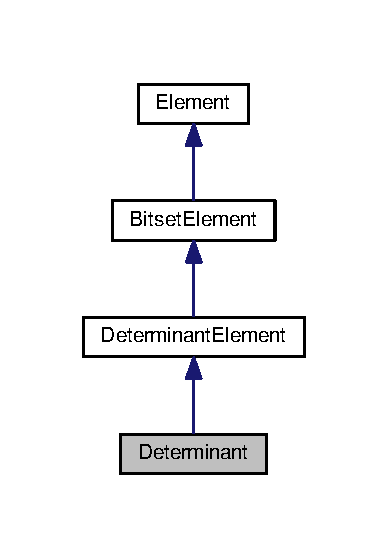
\includegraphics[width=186pt]{classDeterminant__inherit__graph}
\end{center}
\end{figure}


Collaboration diagram for Determinant\+:
\nopagebreak
\begin{figure}[H]
\begin{center}
\leavevmode
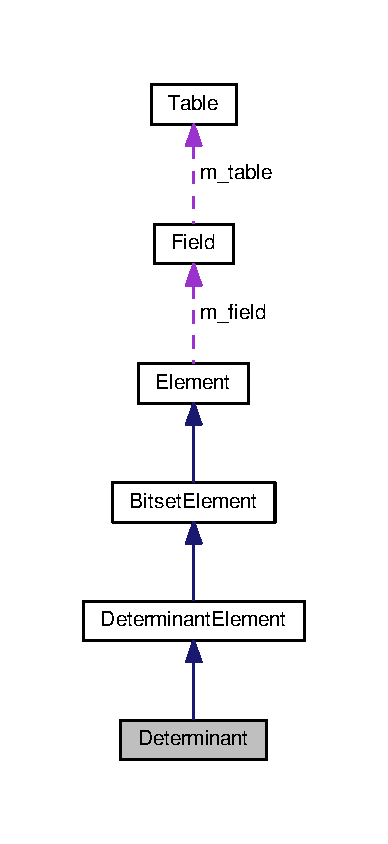
\includegraphics[width=186pt]{classDeterminant__coll__graph}
\end{center}
\end{figure}
\subsection*{Public Member Functions}
\begin{DoxyCompactItemize}
\item 
{\bfseries Determinant} (size\+\_\+t nsite)\hypertarget{classDeterminant_ab4bc213a4be8141ad78a5b89e55f6365}{}\label{classDeterminant_ab4bc213a4be8141ad78a5b89e55f6365}

\item 
\hyperlink{classDeterminant}{Determinant} \& {\bfseries operator=} (const \hyperlink{classDeterminantElement}{Determinant\+Element} \&rhs)\hypertarget{classDeterminant_a7e7423bd3b83b14a25039b70246f0bb7}{}\label{classDeterminant_a7e7423bd3b83b14a25039b70246f0bb7}

\item 
\hyperlink{classDeterminant}{Determinant} \& {\bfseries operator=} (const \hyperlink{classDeterminant}{Determinant} \&rhs)\hypertarget{classDeterminant_a4c2983ed67891b319c2fd9d7f518b698}{}\label{classDeterminant_a4c2983ed67891b319c2fd9d7f518b698}

\item 
{\bfseries Determinant} (const \hyperlink{classDeterminant}{Determinant} \&obj)\hypertarget{classDeterminant_a67cbe0742c6b5f3a211aff76112de960}{}\label{classDeterminant_a67cbe0742c6b5f3a211aff76112de960}

\end{DoxyCompactItemize}
\subsection*{Additional Inherited Members}


The documentation for this class was generated from the following file\+:\begin{DoxyCompactItemize}
\item 
/home/teamcity/\+Team\+City/build\+Agent/work/5343cdffda4690e5/src/core/fermion/Determinant.\+h\end{DoxyCompactItemize}

\hypertarget{classDeterminantClrEnumerator}{}\section{Determinant\+Clr\+Enumerator Class Reference}
\label{classDeterminantClrEnumerator}\index{Determinant\+Clr\+Enumerator@{Determinant\+Clr\+Enumerator}}


Inheritance diagram for Determinant\+Clr\+Enumerator\+:
% FIG 0


Collaboration diagram for Determinant\+Clr\+Enumerator\+:
% FIG 1
\subsection*{Public Member Functions}
\begin{DoxyCompactItemize}
\item 
{\bfseries Determinant\+Clr\+Enumerator} (const \hyperlink{classDeterminantElement}{Determinant\+Element} \&data1, \hyperlink{classEnumerator}{Enumerator}$<$ size\+\_\+t $>$ $\ast$subsequent=nullptr, size\+\_\+t offset=0)\hypertarget{classDeterminantClrEnumerator_ac62b7f64a2dd7e40b30545cf0d9344df}{}\label{classDeterminantClrEnumerator_ac62b7f64a2dd7e40b30545cf0d9344df}

\end{DoxyCompactItemize}
\subsection*{Additional Inherited Members}


The documentation for this class was generated from the following file\+:\begin{DoxyCompactItemize}
\item 
/home/teamcity/\+Team\+City/build\+Agent/work/5343cdffda4690e5/src/core/enumerator/Bitset\+Enumerator.\+h\end{DoxyCompactItemize}

\hypertarget{classDeterminantElement}{}\section{Determinant\+Element Class Reference}
\label{classDeterminantElement}\index{Determinant\+Element@{Determinant\+Element}}


Inheritance diagram for Determinant\+Element\+:
\nopagebreak
\begin{figure}[H]
\begin{center}
\leavevmode
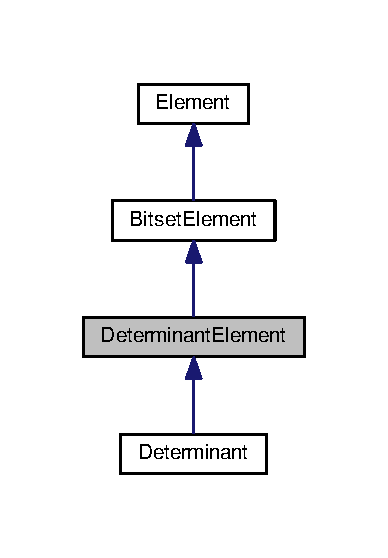
\includegraphics[width=186pt]{classDeterminantElement__inherit__graph}
\end{center}
\end{figure}


Collaboration diagram for Determinant\+Element\+:
\nopagebreak
\begin{figure}[H]
\begin{center}
\leavevmode
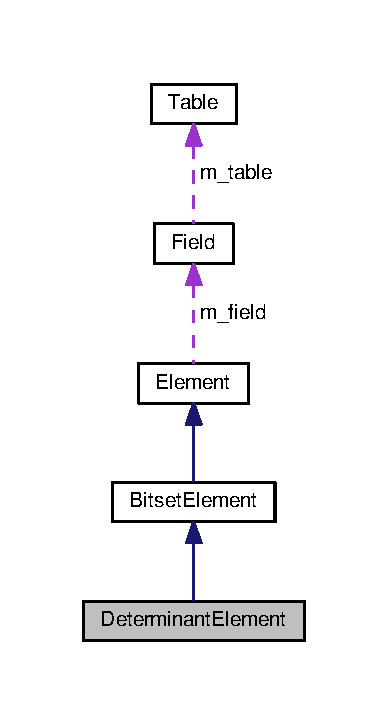
\includegraphics[width=186pt]{classDeterminantElement__coll__graph}
\end{center}
\end{figure}
\subsection*{Classes}
\begin{DoxyCompactItemize}
\item 
class \hyperlink{classDeterminantElement_1_1AntiDatawordEnumerator}{Anti\+Dataword\+Enumerator}
\item 
class \hyperlink{classDeterminantElement_1_1DatawordEnumerator}{Dataword\+Enumerator}
\end{DoxyCompactItemize}
\subsection*{Public Types}
\begin{DoxyCompactItemize}
\item 
typedef \hyperlink{classDeterminantField}{Determinant\+Field} {\bfseries Field\+\_\+T}\hypertarget{classDeterminantElement_a35ba407ecc76258d039bf7ef1bcefe8a}{}\label{classDeterminantElement_a35ba407ecc76258d039bf7ef1bcefe8a}

\end{DoxyCompactItemize}
\subsection*{Public Member Functions}
\begin{DoxyCompactItemize}
\item 
{\bfseries Determinant\+Element} (\hyperlink{classDeterminantField}{Determinant\+Field} $\ast$field, char $\ast$begin)\hypertarget{classDeterminantElement_afa05f6796b4f932f58ef7d153e49c05b}{}\label{classDeterminantElement_afa05f6796b4f932f58ef7d153e49c05b}

\item 
virtual std\+::string {\bfseries to\+\_\+string} () const \hypertarget{classDeterminantElement_af3680358fd1c637e09595d352d1cbc7e}{}\label{classDeterminantElement_af3680358fd1c637e09595d352d1cbc7e}

\item 
void {\bfseries set} (const size\+\_\+t \&ispin, const size\+\_\+t \&iorb)\hypertarget{classDeterminantElement_af950f1affe4063cc566060c9f1fa4f39}{}\label{classDeterminantElement_af950f1affe4063cc566060c9f1fa4f39}

\item 
void {\bfseries set} (const defs\+::inds \&ispinorbs)\hypertarget{classDeterminantElement_a2409ff9d9478c04fbd08e8859ac26555}{}\label{classDeterminantElement_a2409ff9d9478c04fbd08e8859ac26555}

\item 
void {\bfseries clr} (const size\+\_\+t \&ispin, const size\+\_\+t \&iorb)\hypertarget{classDeterminantElement_aaa0f8aa17b2fd38321301b515c80211d}{}\label{classDeterminantElement_aaa0f8aa17b2fd38321301b515c80211d}

\item 
bool {\bfseries get} (const size\+\_\+t \&ispin, const size\+\_\+t \&iorb) const \hypertarget{classDeterminantElement_ad0f34527d28f3d3a5c65f1035e9b08f9}{}\label{classDeterminantElement_ad0f34527d28f3d3a5c65f1035e9b08f9}

\item 
size\+\_\+t {\bfseries nsite} () const \hypertarget{classDeterminantElement_a0173c3c47f5140360769ab8d5b7a1505}{}\label{classDeterminantElement_a0173c3c47f5140360769ab8d5b7a1505}

\item 
void {\bfseries excite} (const size\+\_\+t \&i, const size\+\_\+t \&j)\hypertarget{classDeterminantElement_a6233e3f402771d9abfd784d104a85a77}{}\label{classDeterminantElement_a6233e3f402771d9abfd784d104a85a77}

\item 
void {\bfseries excite} (const size\+\_\+t \&i, const size\+\_\+t \&j, const size\+\_\+t \&k, const size\+\_\+t \&l)\hypertarget{classDeterminantElement_a73bef3958f537648c40bebbda88f36e7}{}\label{classDeterminantElement_a73bef3958f537648c40bebbda88f36e7}

\item 
int {\bfseries spin} () const \hypertarget{classDeterminantElement_a86954e3d0482cd3d0d2af545d630272c}{}\label{classDeterminantElement_a86954e3d0482cd3d0d2af545d630272c}

\item 
int {\bfseries nalpha} () const \hypertarget{classDeterminantElement_a772391a2a03e5cf5f2af76d4477c625e}{}\label{classDeterminantElement_a772391a2a03e5cf5f2af76d4477c625e}

\end{DoxyCompactItemize}
\subsection*{Additional Inherited Members}


The documentation for this class was generated from the following files\+:\begin{DoxyCompactItemize}
\item 
/home/teamcity/\+Team\+City/build\+Agent/work/5343cdffda4690e5/src/core/table/Determinant\+Field.\+h\item 
/home/teamcity/\+Team\+City/build\+Agent/work/5343cdffda4690e5/src/core/table/Determinant\+Field.\+cpp\end{DoxyCompactItemize}

\hypertarget{classDeterminantEnumerator}{}\section{Determinant\+Enumerator$<$ op $>$ Class Template Reference}
\label{classDeterminantEnumerator}\index{Determinant\+Enumerator$<$ op $>$@{Determinant\+Enumerator$<$ op $>$}}


Inheritance diagram for Determinant\+Enumerator$<$ op $>$\+:\nopagebreak
\begin{figure}[H]
\begin{center}
\leavevmode
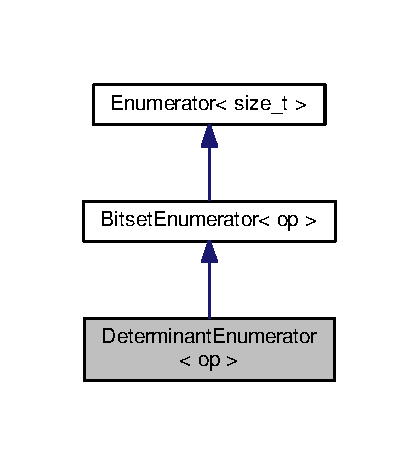
\includegraphics[width=201pt]{classDeterminantEnumerator__inherit__graph}
\end{center}
\end{figure}


Collaboration diagram for Determinant\+Enumerator$<$ op $>$\+:\nopagebreak
\begin{figure}[H]
\begin{center}
\leavevmode
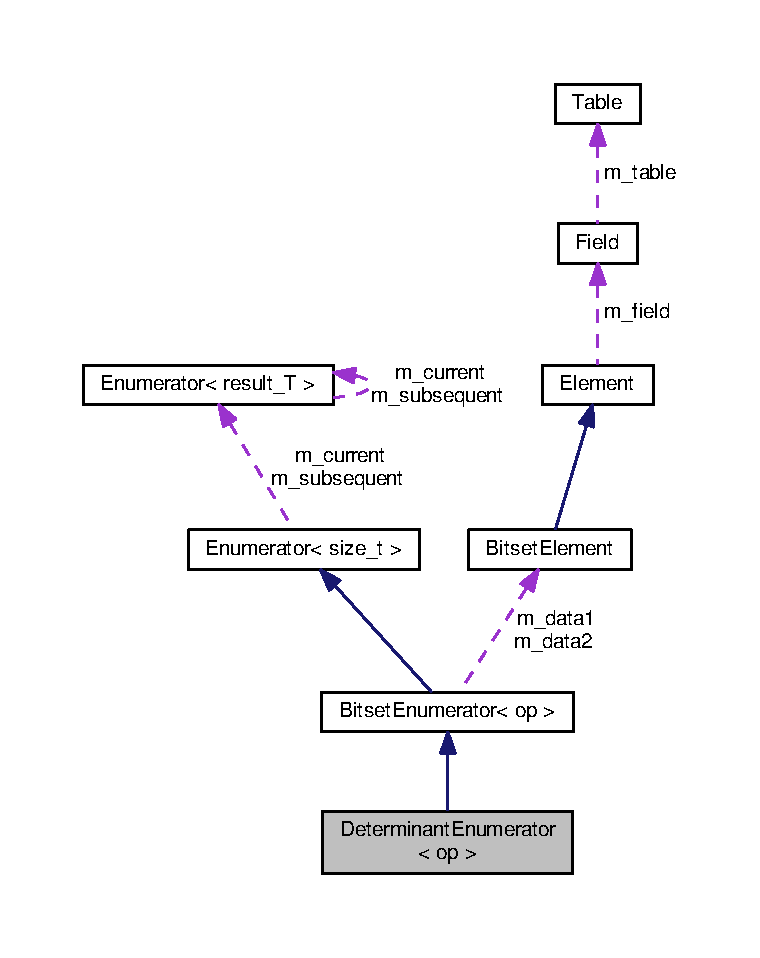
\includegraphics[width=350pt]{classDeterminantEnumerator__coll__graph}
\end{center}
\end{figure}
\subsection*{Public Member Functions}
\begin{DoxyCompactItemize}
\item 
{\bfseries Determinant\+Enumerator} (const \hyperlink{classDeterminantElement}{Determinant\+Element} \&data1, const \hyperlink{classDeterminantElement}{Determinant\+Element} \&data2, \hyperlink{classEnumerator}{Enumerator}$<$ size\+\_\+t $>$ $\ast$subsequent=nullptr, size\+\_\+t offset=0)\hypertarget{classDeterminantEnumerator_a30c99d5c81de8d12caf012f14c1af129}{}\label{classDeterminantEnumerator_a30c99d5c81de8d12caf012f14c1af129}

\item 
bool {\bfseries next\+\_\+element} (size\+\_\+t \&result) override\hypertarget{classDeterminantEnumerator_ab3027854ee62ae607d7326f3cf65553a}{}\label{classDeterminantEnumerator_ab3027854ee62ae607d7326f3cf65553a}

\end{DoxyCompactItemize}
\subsection*{Additional Inherited Members}


The documentation for this class was generated from the following file\+:\begin{DoxyCompactItemize}
\item 
/home/teamcity/\+Team\+City/build\+Agent/work/5343cdffda4690e5/src/core/enumerator/Bitset\+Enumerator.\+h\end{DoxyCompactItemize}

\hypertarget{classDeterminantField}{}\section{Determinant\+Field Class Reference}
\label{classDeterminantField}\index{Determinant\+Field@{Determinant\+Field}}


Inheritance diagram for Determinant\+Field\+:
\nopagebreak
\begin{figure}[H]
\begin{center}
\leavevmode
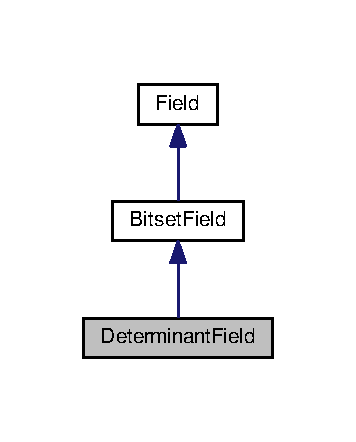
\includegraphics[width=171pt]{classDeterminantField__inherit__graph}
\end{center}
\end{figure}


Collaboration diagram for Determinant\+Field\+:
\nopagebreak
\begin{figure}[H]
\begin{center}
\leavevmode
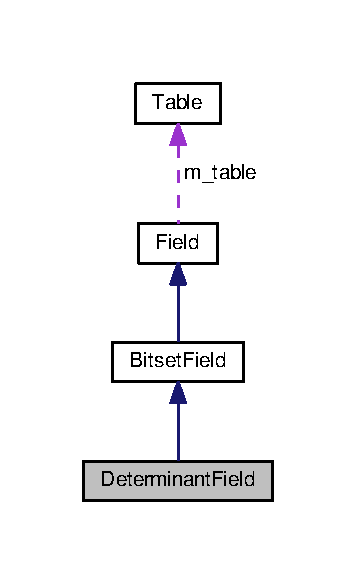
\includegraphics[width=171pt]{classDeterminantField__coll__graph}
\end{center}
\end{figure}
\subsection*{Public Member Functions}
\begin{DoxyCompactItemize}
\item 
{\bfseries Determinant\+Field} (\hyperlink{classTable}{Table} $\ast$table, size\+\_\+t nelement, size\+\_\+t nsite, const std\+::string \&description=\char`\"{}\char`\"{})\hypertarget{classDeterminantField_a4a78bd11b89a0791bea26e583e1771b4}{}\label{classDeterminantField_a4a78bd11b89a0791bea26e583e1771b4}

\item 
\hyperlink{classDeterminantElement}{Determinant\+Element} {\bfseries operator()} (const size\+\_\+t \&irow, const size\+\_\+t \&isegment=0, const size\+\_\+t \&ielement=0)\hypertarget{classDeterminantField_ae40d526423cefc0be2ba2f39b1ccd3db}{}\label{classDeterminantField_ae40d526423cefc0be2ba2f39b1ccd3db}

\item 
std\+::string {\bfseries to\+\_\+string} (size\+\_\+t irow, size\+\_\+t isegment, size\+\_\+t ielement) override\hypertarget{classDeterminantField_a6a3a2a1523d6f7a1d49e533be4298739}{}\label{classDeterminantField_a6a3a2a1523d6f7a1d49e533be4298739}

\end{DoxyCompactItemize}
\subsection*{Public Attributes}
\begin{DoxyCompactItemize}
\item 
const size\+\_\+t {\bfseries m\+\_\+nsite}\hypertarget{classDeterminantField_a8892acc9446867cf8a21f24ec4ce6b88}{}\label{classDeterminantField_a8892acc9446867cf8a21f24ec4ce6b88}

\end{DoxyCompactItemize}
\subsection*{Additional Inherited Members}


The documentation for this class was generated from the following files\+:\begin{DoxyCompactItemize}
\item 
/home/teamcity/\+Team\+City/build\+Agent/work/5343cdffda4690e5/src/core/table/Determinant\+Field.\+h\item 
/home/teamcity/\+Team\+City/build\+Agent/work/5343cdffda4690e5/src/core/table/Determinant\+Field.\+cpp\end{DoxyCompactItemize}

\hypertarget{classDeterminantSampler}{}\doxysection{Determinant\+Sampler Class Reference}
\label{classDeterminantSampler}\index{DeterminantSampler@{DeterminantSampler}}
\doxysubsection*{Public Types}
\begin{DoxyCompactItemize}
\item 
\mbox{\Hypertarget{classDeterminantSampler_ae5a3525e6db38b07812ae2eea419fb3d}\label{classDeterminantSampler_ae5a3525e6db38b07812ae2eea419fb3d}} 
enum {\bfseries Outcome} \{ {\bfseries no\+\_\+excitations}, 
{\bfseries single\+\_\+excitation}, 
{\bfseries double\+\_\+excitation}, 
{\bfseries both\+\_\+excitations}
 \}
\end{DoxyCompactItemize}
\doxysubsection*{Public Member Functions}
\begin{DoxyCompactItemize}
\item 
\mbox{\Hypertarget{classDeterminantSampler_abb078a6f42fccf201b920c09ba76046b}\label{classDeterminantSampler_abb078a6f42fccf201b920c09ba76046b}} 
{\bfseries Determinant\+Sampler} (const \mbox{\hyperlink{classHeatBathSampler}{Heat\+Bath\+Sampler}} \&precomputed)
\item 
\mbox{\Hypertarget{classDeterminantSampler_a2b2dfe2ed07235bb2b4164f992c2bdf2}\label{classDeterminantSampler_a2b2dfe2ed07235bb2b4164f992c2bdf2}} 
void {\bfseries update} (const \mbox{\hyperlink{classDeterminantElement}{Determinant\+Element}} \&det)
\item 
\mbox{\Hypertarget{classDeterminantSampler_a19293ae543a7207feea79427e1f55727}\label{classDeterminantSampler_a19293ae543a7207feea79427e1f55727}} 
void {\bfseries set\+\_\+\+P1} (std\+::vector$<$ defs\+::prob\+\_\+t $>$ \&P1)
\item 
\mbox{\Hypertarget{classDeterminantSampler_a3c74bd49213c83a20b387cc2a9421505}\label{classDeterminantSampler_a3c74bd49213c83a20b387cc2a9421505}} 
void {\bfseries set\+\_\+\+P2} (std\+::vector$<$ defs\+::prob\+\_\+t $>$ \&P2, const size\+\_\+t \&p)
\item 
\mbox{\Hypertarget{classDeterminantSampler_a0dc046b3b9ecfaae06c89c1c1933460f}\label{classDeterminantSampler_a0dc046b3b9ecfaae06c89c1c1933460f}} 
void {\bfseries draw\+\_\+pq} (size\+\_\+t \&p, size\+\_\+t \&q)
\item 
\mbox{\Hypertarget{classDeterminantSampler_ae9eb1d7f8e68b1dc5da726ed7b2c8ed7}\label{classDeterminantSampler_ae9eb1d7f8e68b1dc5da726ed7b2c8ed7}} 
void {\bfseries draw\+\_\+pq} (size\+\_\+t \&p, size\+\_\+t \&q, defs\+::prob\+\_\+t \&prob)
\item 
\mbox{\Hypertarget{classDeterminantSampler_ace140c1bcbf11e1f9b1ed147bfa915b8}\label{classDeterminantSampler_ace140c1bcbf11e1f9b1ed147bfa915b8}} 
void {\bfseries draw\+\_\+r} (const size\+\_\+t \&p, const size\+\_\+t \&q, size\+\_\+t \&r)
\item 
\mbox{\Hypertarget{classDeterminantSampler_a12a39a2f854b9da9802bf2b51a2caa3a}\label{classDeterminantSampler_a12a39a2f854b9da9802bf2b51a2caa3a}} 
void {\bfseries draw\+\_\+r} (const size\+\_\+t \&p, const size\+\_\+t \&q, size\+\_\+t \&r, defs\+::prob\+\_\+t \&prob)
\item 
\mbox{\Hypertarget{classDeterminantSampler_a9764cc8221fb895caf9014c07857b5eb}\label{classDeterminantSampler_a9764cc8221fb895caf9014c07857b5eb}} 
void {\bfseries draw\+\_\+pqr} (size\+\_\+t \&p, size\+\_\+t \&q, size\+\_\+t \&r)
\item 
\mbox{\Hypertarget{classDeterminantSampler_a479a10cf7c973805e1a70ac5c09654dd}\label{classDeterminantSampler_a479a10cf7c973805e1a70ac5c09654dd}} 
void {\bfseries draw\+\_\+pqr} (size\+\_\+t \&p, size\+\_\+t \&q, size\+\_\+t \&r, defs\+::prob\+\_\+t \&prob)
\item 
\mbox{\Hypertarget{classDeterminantSampler_a6c7b1d4a7f2acf36ec518346172a5dc3}\label{classDeterminantSampler_a6c7b1d4a7f2acf36ec518346172a5dc3}} 
void {\bfseries draw\+\_\+s} (const size\+\_\+t \&p, const size\+\_\+t \&q, const size\+\_\+t \&r, size\+\_\+t \&s)
\item 
\mbox{\Hypertarget{classDeterminantSampler_af71dfd0ce319f32ff71e5595164cbfc6}\label{classDeterminantSampler_af71dfd0ce319f32ff71e5595164cbfc6}} 
void {\bfseries draw\+\_\+s} (const size\+\_\+t \&p, const size\+\_\+t \&q, const size\+\_\+t \&r, size\+\_\+t \&s, defs\+::prob\+\_\+t \&prob)
\item 
\mbox{\Hypertarget{classDeterminantSampler_a0ba6e15b20e2412fb07d0414e17dddfe}\label{classDeterminantSampler_a0ba6e15b20e2412fb07d0414e17dddfe}} 
void {\bfseries draw} (size\+\_\+t \&p, size\+\_\+t \&q, size\+\_\+t \&r, size\+\_\+t \&s, defs\+::prob\+\_\+t \&prob\+\_\+single, defs\+::prob\+\_\+t \&prob\+\_\+double, defs\+::ham\+\_\+t \&helement\+\_\+single, defs\+::ham\+\_\+t \&helement\+\_\+double)
\item 
\mbox{\Hypertarget{classDeterminantSampler_afda44a408c15e263eecb24e81350c29c}\label{classDeterminantSampler_afda44a408c15e263eecb24e81350c29c}} 
void {\bfseries draw} ()
\item 
\mbox{\Hypertarget{classDeterminantSampler_aac31f89b9879f341b72f092c0188b70f}\label{classDeterminantSampler_aac31f89b9879f341b72f092c0188b70f}} 
bool {\bfseries single\+\_\+generated} () const
\item 
\mbox{\Hypertarget{classDeterminantSampler_af786eddca18a703aca6406e6d0b59696}\label{classDeterminantSampler_af786eddca18a703aca6406e6d0b59696}} 
bool {\bfseries double\+\_\+generated} () const
\item 
\mbox{\Hypertarget{classDeterminantSampler_a495794b8f68f0dfec00cd2162123dd78}\label{classDeterminantSampler_a495794b8f68f0dfec00cd2162123dd78}} 
\mbox{\hyperlink{classAntisymConnection}{Antisym\+Connection}} \& {\bfseries get\+\_\+single} ()
\item 
\mbox{\Hypertarget{classDeterminantSampler_a8a6ec6cd34ec3dbed33d550b03142a44}\label{classDeterminantSampler_a8a6ec6cd34ec3dbed33d550b03142a44}} 
\mbox{\hyperlink{classAntisymConnection}{Antisym\+Connection}} \& {\bfseries get\+\_\+double} ()
\item 
\mbox{\Hypertarget{classDeterminantSampler_a0433b57f3cb61e4c438f567dc8bbcb6b}\label{classDeterminantSampler_a0433b57f3cb61e4c438f567dc8bbcb6b}} 
const \mbox{\hyperlink{classDeterminant}{Determinant}} \& {\bfseries get\+\_\+single\+\_\+dst\+\_\+det} ()
\item 
\mbox{\Hypertarget{classDeterminantSampler_a971cee489d38916d37b8775b6badf55a}\label{classDeterminantSampler_a971cee489d38916d37b8775b6badf55a}} 
const \mbox{\hyperlink{classDeterminant}{Determinant}} \& {\bfseries get\+\_\+double\+\_\+dst\+\_\+det} ()
\item 
\mbox{\Hypertarget{classDeterminantSampler_a2cd9d220ea45808d82abedc47da53880}\label{classDeterminantSampler_a2cd9d220ea45808d82abedc47da53880}} 
const defs\+::prob\+\_\+t \& {\bfseries get\+\_\+single\+\_\+prob} () const
\item 
\mbox{\Hypertarget{classDeterminantSampler_a144ebb11c70698ebaff326ba71593b45}\label{classDeterminantSampler_a144ebb11c70698ebaff326ba71593b45}} 
const defs\+::prob\+\_\+t \& {\bfseries get\+\_\+double\+\_\+prob} () const
\end{DoxyCompactItemize}


The documentation for this class was generated from the following files\+:\begin{DoxyCompactItemize}
\item 
/home/teamcity/\+Team\+City/build\+Agent/work/5343cdffda4690e5/src/core/heatbath/Determinant\+Sampler.\+h\item 
/home/teamcity/\+Team\+City/build\+Agent/work/5343cdffda4690e5/src/core/heatbath/Determinant\+Sampler.\+cpp\end{DoxyCompactItemize}

\hypertarget{classDeterminantSetEnumerator}{}\section{Determinant\+Set\+Enumerator Class Reference}
\label{classDeterminantSetEnumerator}\index{Determinant\+Set\+Enumerator@{Determinant\+Set\+Enumerator}}


Inheritance diagram for Determinant\+Set\+Enumerator\+:\nopagebreak
\begin{figure}[H]
\begin{center}
\leavevmode
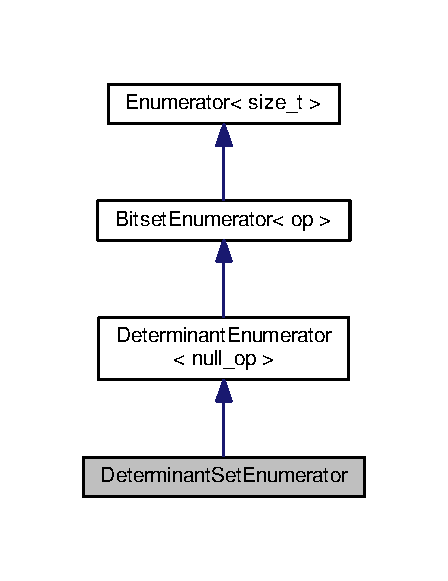
\includegraphics[width=215pt]{classDeterminantSetEnumerator__inherit__graph}
\end{center}
\end{figure}


Collaboration diagram for Determinant\+Set\+Enumerator\+:\nopagebreak
\begin{figure}[H]
\begin{center}
\leavevmode
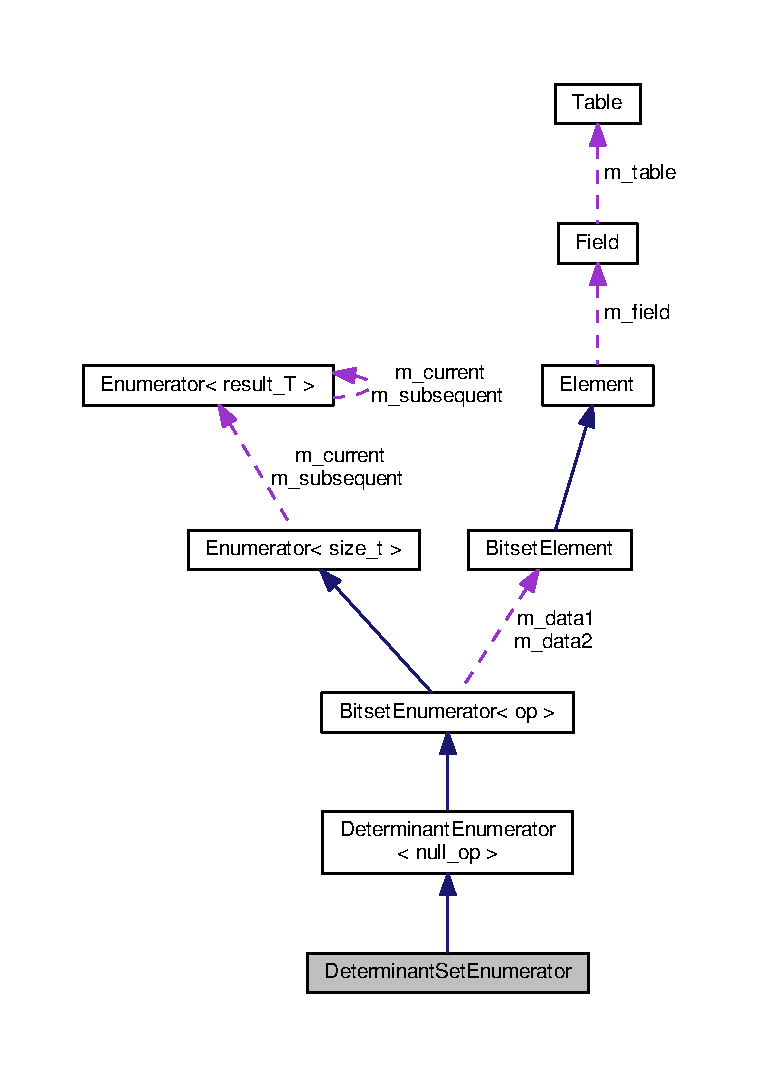
\includegraphics[width=350pt]{classDeterminantSetEnumerator__coll__graph}
\end{center}
\end{figure}
\subsection*{Public Member Functions}
\begin{DoxyCompactItemize}
\item 
{\bfseries Determinant\+Set\+Enumerator} (const \hyperlink{classDeterminantElement}{Determinant\+Element} \&data1, \hyperlink{classEnumerator}{Enumerator}$<$ size\+\_\+t $>$ $\ast$subsequent=nullptr, size\+\_\+t offset=0)\hypertarget{classDeterminantSetEnumerator_ad0f4b145140c6f643c0a1d849b2cd527}{}\label{classDeterminantSetEnumerator_ad0f4b145140c6f643c0a1d849b2cd527}

\end{DoxyCompactItemize}
\subsection*{Additional Inherited Members}


The documentation for this class was generated from the following file\+:\begin{DoxyCompactItemize}
\item 
/home/teamcity/\+Team\+City/build\+Agent/work/5343cdffda4690e5/src/core/enumerator/Bitset\+Enumerator.\+h\end{DoxyCompactItemize}

\hypertarget{classDeterministicSubspace}{}\doxysection{Deterministic\+Subspace Class Reference}
\label{classDeterministicSubspace}\index{DeterministicSubspace@{DeterministicSubspace}}
\doxysubsection*{Public Member Functions}
\begin{DoxyCompactItemize}
\item 
\mbox{\Hypertarget{classDeterministicSubspace_a13fdd0e23b39605b254db4a00b3b34de}\label{classDeterministicSubspace_a13fdd0e23b39605b254db4a00b3b34de}} 
void {\bfseries gather\+\_\+and\+\_\+project} ()
\item 
\mbox{\Hypertarget{classDeterministicSubspace_a694d65435340cc23a6c67d6534f04ba7}\label{classDeterministicSubspace_a694d65435340cc23a6c67d6534f04ba7}} 
void {\bfseries rayleigh\+\_\+quotient} (\mbox{\hyperlink{classHybrid}{Hybrid}}$<$ defs\+::ham\+\_\+t $>$ \&num, \mbox{\hyperlink{classHybrid}{Hybrid}}$<$ defs\+::ham\+\_\+comp\+\_\+t $>$ \&norm\+\_\+square)
\item 
\mbox{\Hypertarget{classDeterministicSubspace_a22cbdd2efc16aa61722c976dbb6297f9}\label{classDeterministicSubspace_a22cbdd2efc16aa61722c976dbb6297f9}} 
defs\+::ham\+\_\+comp\+\_\+t {\bfseries update\+\_\+weights} (const double \&tau)
\item 
\mbox{\Hypertarget{classDeterministicSubspace_a6872430fe91bcd2d55c23f13929e7ab1}\label{classDeterministicSubspace_a6872430fe91bcd2d55c23f13929e7ab1}} 
{\bfseries Deterministic\+Subspace} (\mbox{\hyperlink{structWalkerList}{Walker\+List}} $\ast$walker\+\_\+list)
\item 
\mbox{\Hypertarget{classDeterministicSubspace_aea0ef2bad6d6ab5c1aea0a4da64e0818}\label{classDeterministicSubspace_aea0ef2bad6d6ab5c1aea0a4da64e0818}} 
void {\bfseries add\+\_\+determinant} (size\+\_\+t irow\+\_\+walker\+\_\+list)
\item 
\mbox{\Hypertarget{classDeterministicSubspace_ad7788b62b08026bafb98c20cbd2d3f1f}\label{classDeterministicSubspace_ad7788b62b08026bafb98c20cbd2d3f1f}} 
const size\+\_\+t \& {\bfseries nrow\+\_\+local} () const
\item 
\mbox{\Hypertarget{classDeterministicSubspace_ab020981773f467ad7aaa781b7322406b}\label{classDeterministicSubspace_ab020981773f467ad7aaa781b7322406b}} 
const size\+\_\+t \& {\bfseries nrow\+\_\+full} () const
\item 
\mbox{\Hypertarget{classDeterministicSubspace_aec2fe67ca62dee312a4a7c878ebef365}\label{classDeterministicSubspace_aec2fe67ca62dee312a4a7c878ebef365}} 
\mbox{\hyperlink{classDeterminantElement}{Determinant\+Element}} {\bfseries local\+\_\+det} (const size\+\_\+t \&irow) const
\item 
\mbox{\Hypertarget{classDeterministicSubspace_a1c18080fde4882a7652959c6be741280}\label{classDeterministicSubspace_a1c18080fde4882a7652959c6be741280}} 
void {\bfseries build\+\_\+from\+\_\+whole\+\_\+walker\+\_\+list} (\mbox{\hyperlink{classHamiltonian}{Hamiltonian}} $\ast$ham)
\item 
\mbox{\Hypertarget{classDeterministicSubspace_a72266a2e0e0098674f3b370577739772}\label{classDeterministicSubspace_a72266a2e0e0098674f3b370577739772}} 
void {\bfseries build\+\_\+from\+\_\+det\+\_\+connections} (const \mbox{\hyperlink{classDeterminantElement}{Determinant\+Element}} \&ref, \mbox{\hyperlink{classHamiltonian}{Hamiltonian}} $\ast$ham)
\end{DoxyCompactItemize}


The documentation for this class was generated from the following file\+:\begin{DoxyCompactItemize}
\item 
/home/teamcity/\+Team\+City/build\+Agent/work/5343cdffda4690e5/src/core/dynamics/Deterministic\+Subspace.\+h\end{DoxyCompactItemize}

\hypertarget{classDistributed}{}\doxysection{Distributed$<$ T $>$ Class Template Reference}
\label{classDistributed}\index{Distributed$<$ T $>$@{Distributed$<$ T $>$}}


Inheritance diagram for Distributed$<$ T $>$\+:\nopagebreak
\begin{figure}[H]
\begin{center}
\leavevmode
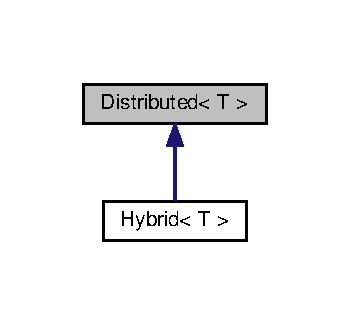
\includegraphics[width=168pt]{classDistributed__inherit__graph}
\end{center}
\end{figure}
\doxysubsection*{Public Member Functions}
\begin{DoxyCompactItemize}
\item 
\mbox{\Hypertarget{classDistributed_afa406491c5c5c40ed5863dc4469e5659}\label{classDistributed_afa406491c5c5c40ed5863dc4469e5659}} 
virtual \mbox{\hyperlink{classDistributed}{Distributed}}$<$ T $>$ \& {\bfseries operator=} (const T \&rhs)
\item 
\mbox{\Hypertarget{classDistributed_a1182ef89565a5569fe0ddd29c4bdcc73}\label{classDistributed_a1182ef89565a5569fe0ddd29c4bdcc73}} 
virtual \mbox{\hyperlink{classDistributed}{Distributed}}$<$ T $>$ \& {\bfseries operator+=} (const T \&rhs)
\item 
\mbox{\Hypertarget{classDistributed_a218d6294ba8ff92a6255a2f4fbc01725}\label{classDistributed_a218d6294ba8ff92a6255a2f4fbc01725}} 
T \& {\bfseries local} ()
\item 
\mbox{\Hypertarget{classDistributed_a701315b13407247153f565a083c8edac}\label{classDistributed_a701315b13407247153f565a083c8edac}} 
T \& {\bfseries reduced} ()
\item 
\mbox{\Hypertarget{classDistributed_a32271aa55f24dabab522859c8bfed13c}\label{classDistributed_a32271aa55f24dabab522859c8bfed13c}} 
T \& {\bfseries mpi\+\_\+sum} ()
\item 
\mbox{\Hypertarget{classDistributed_a5c99add9baedb3f683ff471df3c68cc4}\label{classDistributed_a5c99add9baedb3f683ff471df3c68cc4}} 
T \& {\bfseries mpi\+\_\+max} ()
\item 
\mbox{\Hypertarget{classDistributed_a8fbbf78175911664d72bffd5396d9c97}\label{classDistributed_a8fbbf78175911664d72bffd5396d9c97}} 
T \& {\bfseries mpi\+\_\+min} ()
\item 
\mbox{\Hypertarget{classDistributed_a4c74cb6ab8f16efe7bc74eb8ad1405f3}\label{classDistributed_a4c74cb6ab8f16efe7bc74eb8ad1405f3}} 
T \& {\bfseries mpi\+\_\+bcast} (size\+\_\+t irank)
\end{DoxyCompactItemize}
\doxysubsection*{Protected Attributes}
\begin{DoxyCompactItemize}
\item 
\mbox{\Hypertarget{classDistributed_a72d30e892605cfb0a74688aac65f6e2e}\label{classDistributed_a72d30e892605cfb0a74688aac65f6e2e}} 
T {\bfseries m\+\_\+local} = 0
\item 
\mbox{\Hypertarget{classDistributed_ac5bdb0e490c61aa164b6d060deccb068}\label{classDistributed_ac5bdb0e490c61aa164b6d060deccb068}} 
T {\bfseries m\+\_\+reduced} = std\+::numeric\+\_\+limits$<$T$>$\+::max()
\end{DoxyCompactItemize}


The documentation for this class was generated from the following file\+:\begin{DoxyCompactItemize}
\item 
/home/teamcity/\+Team\+City/build\+Agent/work/5343cdffda4690e5/src/core/parallel/Distributed.\+h\end{DoxyCompactItemize}

\hypertarget{classEigenSolver}{}\doxysection{Eigen\+Solver$<$ T $>$ Class Template Reference}
\label{classEigenSolver}\index{EigenSolver$<$ T $>$@{EigenSolver$<$ T $>$}}
\doxysubsection*{Public Member Functions}
\begin{DoxyCompactItemize}
\item 
\mbox{\Hypertarget{classEigenSolver_af4c7de6d265f452e879a0cb002e85657}\label{classEigenSolver_af4c7de6d265f452e879a0cb002e85657}} 
{\bfseries Eigen\+Solver} (const \mbox{\hyperlink{classMatrix}{Matrix}}$<$ T $>$ \&matrix)
\end{DoxyCompactItemize}
\doxysubsection*{Public Attributes}
\begin{DoxyCompactItemize}
\item 
\mbox{\Hypertarget{classEigenSolver_a258d447b545146a35ebafcdef9666249}\label{classEigenSolver_a258d447b545146a35ebafcdef9666249}} 
\mbox{\hyperlink{classMatrix}{Matrix}}$<$ T $>$ {\bfseries m\+\_\+evecs}
\item 
\mbox{\Hypertarget{classEigenSolver_a99ef6b50732d813bc55cb2195ddc8883}\label{classEigenSolver_a99ef6b50732d813bc55cb2195ddc8883}} 
std\+::vector$<$ typename \mbox{\hyperlink{structconsts_1_1component__t}{consts\+::component\+\_\+t}}$<$ T $>$\+::type $>$ {\bfseries m\+\_\+evals}
\end{DoxyCompactItemize}


The documentation for this class was generated from the following file\+:\begin{DoxyCompactItemize}
\item 
/home/teamcity/\+Team\+City/build\+Agent/work/5343cdffda4690e5/src/core/linalg/Eigen\+Solver.\+h\end{DoxyCompactItemize}

\hypertarget{classElement}{}\section{Element Class Reference}
\label{classElement}\index{Element@{Element}}


Inheritance diagram for Element\+:
\nopagebreak
\begin{figure}[H]
\begin{center}
\leavevmode
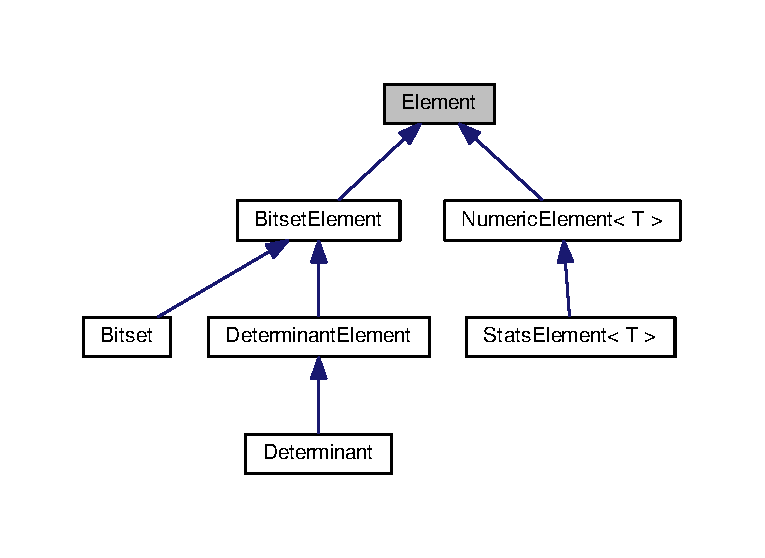
\includegraphics[width=350pt]{classElement__inherit__graph}
\end{center}
\end{figure}


Collaboration diagram for Element\+:
\nopagebreak
\begin{figure}[H]
\begin{center}
\leavevmode
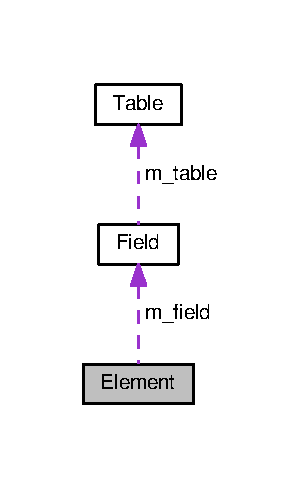
\includegraphics[width=145pt]{classElement__coll__graph}
\end{center}
\end{figure}
\subsection*{Public Types}
\begin{DoxyCompactItemize}
\item 
typedef \hyperlink{classField}{Field} {\bfseries Field\+\_\+T}\hypertarget{classElement_af63af4ed8d72a9bf3abfe86e4cd2e074}{}\label{classElement_af63af4ed8d72a9bf3abfe86e4cd2e074}

\end{DoxyCompactItemize}
\subsection*{Public Member Functions}
\begin{DoxyCompactItemize}
\item 
{\bfseries Element} (\hyperlink{classField}{Field} $\ast$field, char $\ast$begin)\hypertarget{classElement_aed61f8f2a95c9a25046d24a7ed936c3a}{}\label{classElement_aed61f8f2a95c9a25046d24a7ed936c3a}

\item 
virtual size\+\_\+t {\bfseries hash} () const \hypertarget{classElement_a8f46e86dbbd8c7f18c3135742863f3d2}{}\label{classElement_a8f46e86dbbd8c7f18c3135742863f3d2}

\item 
virtual size\+\_\+t {\bfseries size} () const \hypertarget{classElement_a2b8bc248847a45f69cb93965f2a43fa2}{}\label{classElement_a2b8bc248847a45f69cb93965f2a43fa2}

\item 
virtual size\+\_\+t {\bfseries dsize} () const \hypertarget{classElement_a4ce1ba3e934357bd5b9e1bd417641b60}{}\label{classElement_a4ce1ba3e934357bd5b9e1bd417641b60}

\item 
virtual std\+::string {\bfseries to\+\_\+string} ()\hypertarget{classElement_aa9d6b55e58ea084033fb6a96878818da}{}\label{classElement_aa9d6b55e58ea084033fb6a96878818da}

\item 
void {\bfseries print} ()\hypertarget{classElement_a6301e3975df2893421cf3c2dfd64aacb}{}\label{classElement_a6301e3975df2893421cf3c2dfd64aacb}

\item 
bool {\bfseries compatible\+\_\+with} (const \hyperlink{classElement}{Element} \&rhs) const \hypertarget{classElement_ad6dc36d4e46416a511e7ec9d25591f28}{}\label{classElement_ad6dc36d4e46416a511e7ec9d25591f28}

\item 
defs\+::data\+\_\+t \& {\bfseries dataword} (const size\+\_\+t \&idataword) const \hypertarget{classElement_a2ea1802af0c80e1ae4d50dde26b768cd}{}\label{classElement_a2ea1802af0c80e1ae4d50dde26b768cd}

\item 
defs\+::data\+\_\+t {\bfseries get\+\_\+dataword} (const size\+\_\+t \&idataword) const \hypertarget{classElement_a60bffb4917907c0666faa2d63f7a9b03}{}\label{classElement_a60bffb4917907c0666faa2d63f7a9b03}

\item 
defs\+::data\+\_\+t {\bfseries get\+\_\+dataword} (const size\+\_\+t \&idataword, const size\+\_\+t \&nbit) const \hypertarget{classElement_a02754ff9c5e1c6339387c1055bd58ff0}{}\label{classElement_a02754ff9c5e1c6339387c1055bd58ff0}

\item 
defs\+::data\+\_\+t {\bfseries get\+\_\+antidataword} (const size\+\_\+t \&idataword) const \hypertarget{classElement_a71940579c45a95b3e10f4573d04e00bd}{}\label{classElement_a71940579c45a95b3e10f4573d04e00bd}

\item 
defs\+::data\+\_\+t {\bfseries get\+\_\+antidataword} (const size\+\_\+t \&idataword, const size\+\_\+t \&nbit) const \hypertarget{classElement_ae9c0921740d89731f4948c7da1087e4b}{}\label{classElement_ae9c0921740d89731f4948c7da1087e4b}

\item 
int {\bfseries cmp} (const \hyperlink{classElement}{Element} \&rhs) const \hypertarget{classElement_aca814eb1fa9444de47a9709019ccadbb}{}\label{classElement_aca814eb1fa9444de47a9709019ccadbb}

\item 
\hyperlink{classElement}{Element} \& {\bfseries operator=} (const \hyperlink{classElement}{Element} \&rhs)\hypertarget{classElement_a4ad595ed742ac39b2f36fa18ec16097c}{}\label{classElement_a4ad595ed742ac39b2f36fa18ec16097c}

\item 
bool {\bfseries operator==} (const \hyperlink{classElement}{Element} \&rhs) const \hypertarget{classElement_a644fb51331605fc442fb7b8927b4b6b5}{}\label{classElement_a644fb51331605fc442fb7b8927b4b6b5}

\item 
bool {\bfseries operator!=} (const \hyperlink{classElement}{Element} \&rhs) const \hypertarget{classElement_a46ebb3ceb148b0031deeb865d09a1dd6}{}\label{classElement_a46ebb3ceb148b0031deeb865d09a1dd6}

\item 
char $\ast$ {\bfseries begin} () const \hypertarget{classElement_a63b1dc792df7bf96dd2b466989499d33}{}\label{classElement_a63b1dc792df7bf96dd2b466989499d33}

\item 
size\+\_\+t {\bfseries nbit} () const \hypertarget{classElement_a5c3f292dae7456c38a38c8d2e3c0af7a}{}\label{classElement_a5c3f292dae7456c38a38c8d2e3c0af7a}

\item 
void {\bfseries zero} ()\hypertarget{classElement_ad62f7b8502dc5b6083240fd1fadb00ae}{}\label{classElement_ad62f7b8502dc5b6083240fd1fadb00ae}

\item 
virtual bool {\bfseries is\+\_\+zero} () const \hypertarget{classElement_a5ae575a558cb9d1047a6673cefe4daaa}{}\label{classElement_a5ae575a558cb9d1047a6673cefe4daaa}

\item 
const \hyperlink{classField}{Field} $\ast$ {\bfseries field} () const \hypertarget{classElement_ae9d675372592fc556c8a8ed83b81040b}{}\label{classElement_ae9d675372592fc556c8a8ed83b81040b}

\item 
virtual bool {\bfseries is\+\_\+complex} () const \hypertarget{classElement_a311d28ffc677c6cbb7f5383af8dcccf0}{}\label{classElement_a311d28ffc677c6cbb7f5383af8dcccf0}

\end{DoxyCompactItemize}
\subsection*{Protected Attributes}
\begin{DoxyCompactItemize}
\item 
\hyperlink{classField}{Field} $\ast$ {\bfseries m\+\_\+field}\hypertarget{classElement_a32be443e21537c376e41c61a1f3fe302}{}\label{classElement_a32be443e21537c376e41c61a1f3fe302}

\item 
char $\ast$ {\bfseries m\+\_\+begin}\hypertarget{classElement_a43e5c2622b57e837a71fed98190d970a}{}\label{classElement_a43e5c2622b57e837a71fed98190d970a}

\end{DoxyCompactItemize}


The documentation for this class was generated from the following files\+:\begin{DoxyCompactItemize}
\item 
/home/teamcity/\+Team\+City/build\+Agent/work/5343cdffda4690e5/src/core/table/Element.\+h\item 
/home/teamcity/\+Team\+City/build\+Agent/work/5343cdffda4690e5/src/core/table/Element.\+cpp\end{DoxyCompactItemize}

\hypertarget{classEnumerator}{}\section{Enumerator$<$ result\+\_\+T $>$ Class Template Reference}
\label{classEnumerator}\index{Enumerator$<$ result\+\_\+\+T $>$@{Enumerator$<$ result\+\_\+\+T $>$}}


Collaboration diagram for Enumerator$<$ result\+\_\+T $>$\+:
% FIG 0
\subsection*{Public Member Functions}
\begin{DoxyCompactItemize}
\item 
virtual bool {\bfseries next} (result\+\_\+T \&result)\hypertarget{classEnumerator_a8ef6adfaa42901cb007eceef976b2634}{}\label{classEnumerator_a8ef6adfaa42901cb007eceef976b2634}

\item 
virtual bool {\bfseries next} (result\+\_\+T \&result, size\+\_\+t \&i)\hypertarget{classEnumerator_a7f820d7df4327fee1fd3a04ccae5d0bc}{}\label{classEnumerator_a7f820d7df4327fee1fd3a04ccae5d0bc}

\item 
void {\bfseries set\+\_\+subsequent} (\hyperlink{classEnumerator}{Enumerator} $\ast$subsequent)\hypertarget{classEnumerator_ae19248dcf830648c75afcdcc6c2416a5}{}\label{classEnumerator_ae19248dcf830648c75afcdcc6c2416a5}

\item 
bool {\bfseries has\+\_\+subsequent} ()\hypertarget{classEnumerator_a5b31a40fed7827f62084b8f56b48e243}{}\label{classEnumerator_a5b31a40fed7827f62084b8f56b48e243}

\item 
virtual result\+\_\+T {\bfseries default\+\_\+result} ()\hypertarget{classEnumerator_a25a7f1ec275d165f5e37e555861450c5}{}\label{classEnumerator_a25a7f1ec275d165f5e37e555861450c5}

\item 
std\+::vector$<$ result\+\_\+T $>$ {\bfseries enumerate} ()\hypertarget{classEnumerator_a7214314662f3c7ec12f72552a9426ed0}{}\label{classEnumerator_a7214314662f3c7ec12f72552a9426ed0}

\item 
size\+\_\+t {\bfseries count} ()\hypertarget{classEnumerator_a19a17aeb516edf558c9188625c52984a}{}\label{classEnumerator_a19a17aeb516edf558c9188625c52984a}

\item 
bool {\bfseries has\+\_\+fewer\+\_\+than\+\_\+n\+\_\+elements} (size\+\_\+t nmax)\hypertarget{classEnumerator_a1268f2dba0f3d90d1b73f137c488edb8}{}\label{classEnumerator_a1268f2dba0f3d90d1b73f137c488edb8}

\end{DoxyCompactItemize}
\subsection*{Protected Member Functions}
\begin{DoxyCompactItemize}
\item 
{\bfseries Enumerator} (\hyperlink{classEnumerator}{Enumerator} $\ast$subsequent)\hypertarget{classEnumerator_a23d1457bda02cdd5dec929c69a469d29}{}\label{classEnumerator_a23d1457bda02cdd5dec929c69a469d29}

\end{DoxyCompactItemize}
\subsection*{Protected Attributes}
\begin{DoxyCompactItemize}
\item 
\hyperlink{classEnumerator}{Enumerator} $\ast$ {\bfseries m\+\_\+subsequent} = nullptr\hypertarget{classEnumerator_a1535fa29c9f144d93bd47c0be150f45e}{}\label{classEnumerator_a1535fa29c9f144d93bd47c0be150f45e}

\item 
\hyperlink{classEnumerator}{Enumerator} $\ast$ {\bfseries m\+\_\+current} = this\hypertarget{classEnumerator_af6d7d831ebd1fb133a0ea91f60e776fd}{}\label{classEnumerator_af6d7d831ebd1fb133a0ea91f60e776fd}

\end{DoxyCompactItemize}


The documentation for this class was generated from the following file\+:\begin{DoxyCompactItemize}
\item 
/home/teamcity/\+Team\+City/build\+Agent/work/5343cdffda4690e5/src/core/enumerator/Enumerator.\+h\end{DoxyCompactItemize}

\hypertarget{classExactPropagator}{}\doxysection{Exact\+Propagator Class Reference}
\label{classExactPropagator}\index{ExactPropagator@{ExactPropagator}}


Inheritance diagram for Exact\+Propagator\+:\nopagebreak
\begin{figure}[H]
\begin{center}
\leavevmode
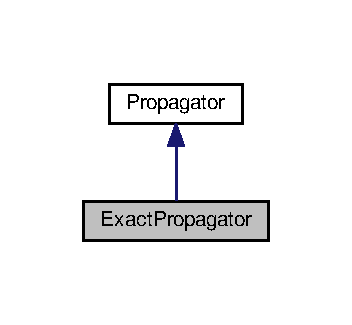
\includegraphics[width=169pt]{classExactPropagator__inherit__graph}
\end{center}
\end{figure}


Collaboration diagram for Exact\+Propagator\+:\nopagebreak
\begin{figure}[H]
\begin{center}
\leavevmode
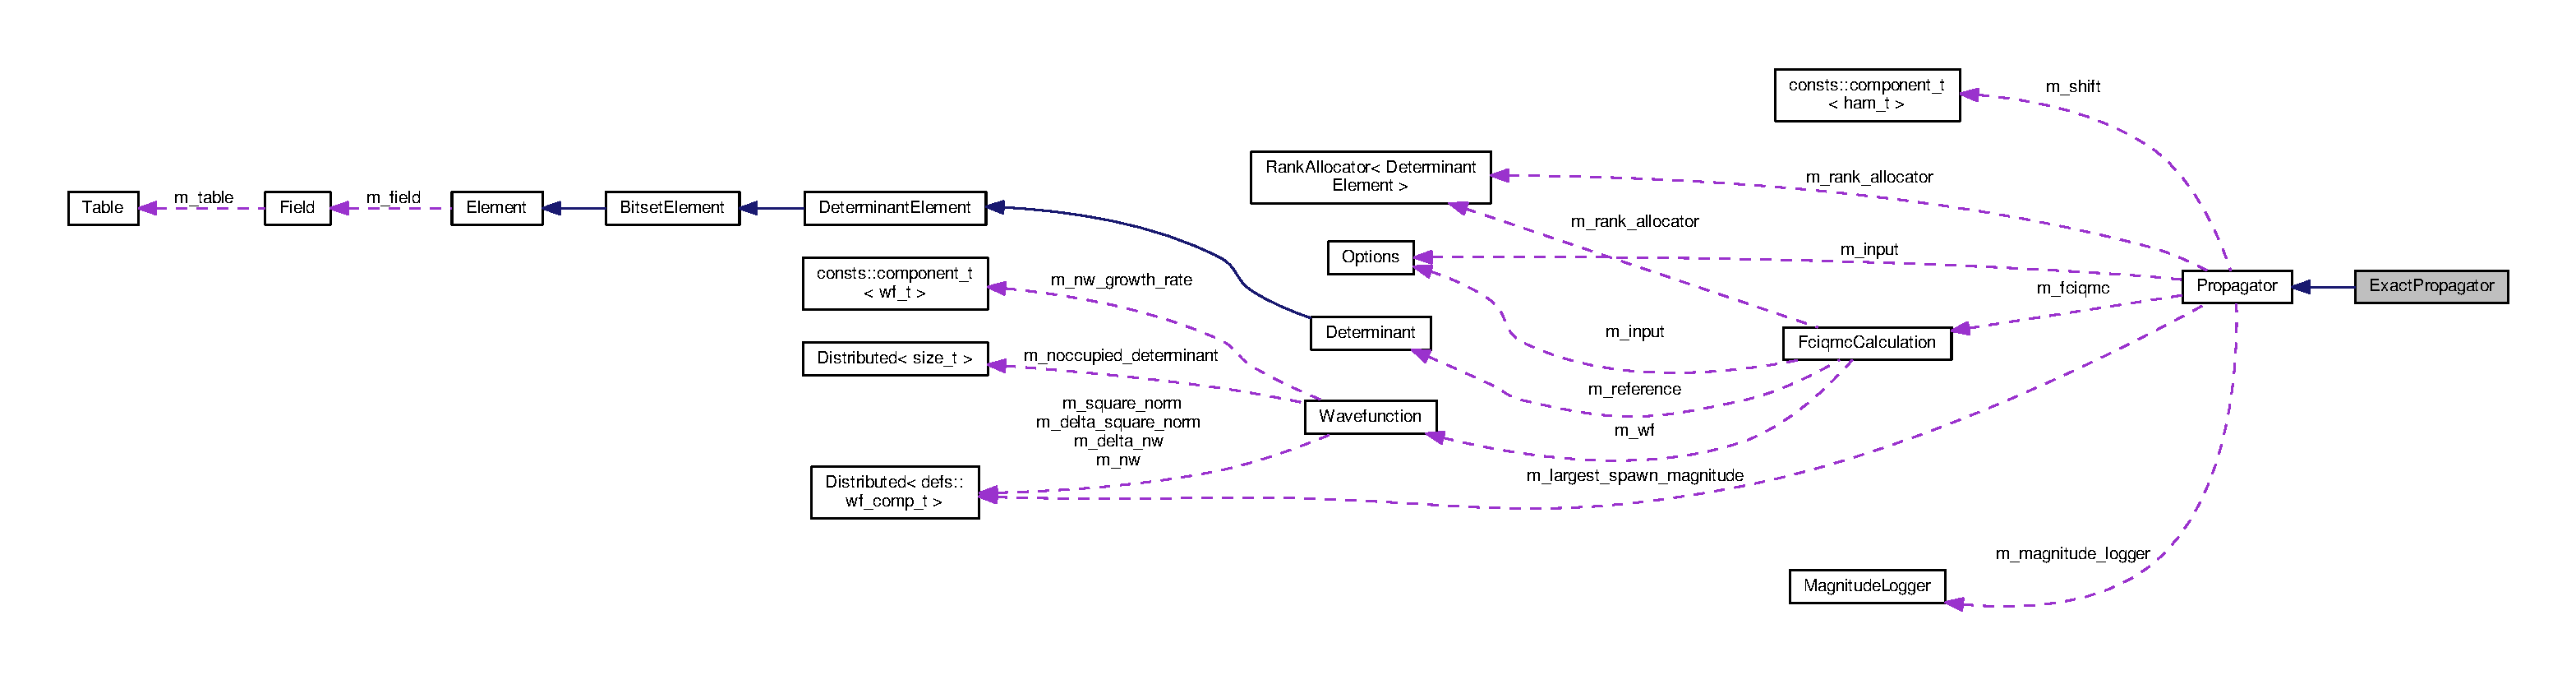
\includegraphics[width=350pt]{classExactPropagator__coll__graph}
\end{center}
\end{figure}
\doxysubsection*{Public Member Functions}
\begin{DoxyCompactItemize}
\item 
\mbox{\Hypertarget{classExactPropagator_a92e82e76311ae33ca8923dc62f75681c}\label{classExactPropagator_a92e82e76311ae33ca8923dc62f75681c}} 
{\bfseries Exact\+Propagator} (\mbox{\hyperlink{classFciqmcCalculation}{Fciqmc\+Calculation}} $\ast$fciqmc)
\item 
\mbox{\Hypertarget{classExactPropagator_abf77c975186a42ce705420706e675150}\label{classExactPropagator_abf77c975186a42ce705420706e675150}} 
void {\bfseries off\+\_\+diagonal} (const \mbox{\hyperlink{classDeterminantElement}{Determinant\+Element}} \&determinant, const \mbox{\hyperlink{classNumericElement}{Numeric\+Element}}$<$ defs\+::ham\+\_\+t $>$ \&weight, \mbox{\hyperlink{structSpawnList}{Spawn\+List}} \&spawn\+\_\+list, bool flag\+\_\+deterministic, bool flag\+\_\+initiator) override
\item 
\mbox{\Hypertarget{classExactPropagator_a3c34937011afc40435b9a75d1345b101}\label{classExactPropagator_a3c34937011afc40435b9a75d1345b101}} 
void {\bfseries diagonal} (const \mbox{\hyperlink{classNumericElement}{Numeric\+Element}}$<$ defs\+::ham\+\_\+comp\+\_\+t $>$ \&hdiag, \mbox{\hyperlink{classNumericElement}{Numeric\+Element}}$<$ defs\+::ham\+\_\+t $>$ \&weight, defs\+::ham\+\_\+comp\+\_\+t \&delta\+\_\+square\+\_\+norm, defs\+::ham\+\_\+comp\+\_\+t \&delta\+\_\+nw) override
\end{DoxyCompactItemize}
\doxysubsection*{Additional Inherited Members}


The documentation for this class was generated from the following files\+:\begin{DoxyCompactItemize}
\item 
/home/teamcity/\+Team\+City/build\+Agent/work/5343cdffda4690e5/src/core/dynamics/Exact\+Propagator.\+h\item 
/home/teamcity/\+Team\+City/build\+Agent/work/5343cdffda4690e5/src/core/dynamics/Exact\+Propagator.\+cpp\end{DoxyCompactItemize}

\hypertarget{classExcitationGenerator}{}\section{Excitation\+Generator Class Reference}
\label{classExcitationGenerator}\index{Excitation\+Generator@{Excitation\+Generator}}


Inheritance diagram for Excitation\+Generator\+:\nopagebreak
\begin{figure}[H]
\begin{center}
\leavevmode
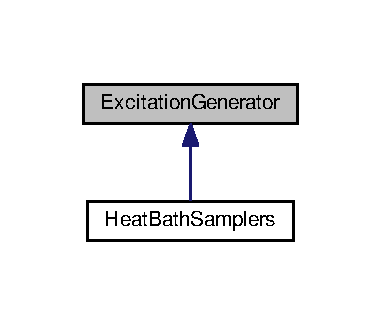
\includegraphics[width=183pt]{classExcitationGenerator__inherit__graph}
\end{center}
\end{figure}


Collaboration diagram for Excitation\+Generator\+:\nopagebreak
\begin{figure}[H]
\begin{center}
\leavevmode
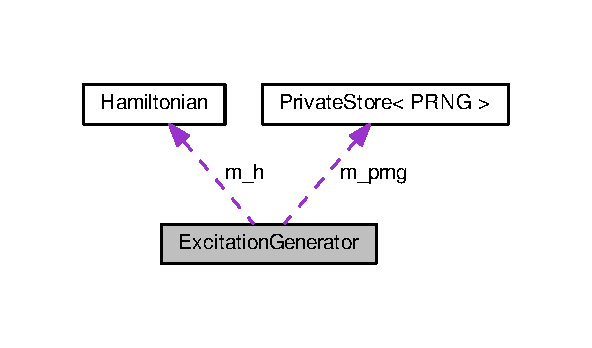
\includegraphics[width=284pt]{classExcitationGenerator__coll__graph}
\end{center}
\end{figure}
\subsection*{Public Member Functions}
\begin{DoxyCompactItemize}
\item 
{\bfseries Excitation\+Generator} (const \hyperlink{classHamiltonian}{Hamiltonian} $\ast$h, \hyperlink{classPrivateStore}{Private\+Store}$<$ \hyperlink{classPRNG}{P\+R\+NG} $>$ \&prng)\hypertarget{classExcitationGenerator_a49314ec4f317bc05a590a58df558aa27}{}\label{classExcitationGenerator_a49314ec4f317bc05a590a58df558aa27}

\item 
virtual bool {\bfseries draw\+\_\+single} (const \hyperlink{classDeterminantElement}{Determinant\+Element} \&src\+\_\+det, \hyperlink{classDeterminantElement}{Determinant\+Element} \&dst\+\_\+det, const \hyperlink{structOccupiedOrbitals}{Occupied\+Orbitals} \&occ, const \hyperlink{structVacantOrbitals}{Vacant\+Orbitals} \&vac, defs\+::prob\+\_\+t \&prob, defs\+::ham\+\_\+t \&helem, \hyperlink{classAntisymConnection}{Antisym\+Connection} \&anticonn)=0\hypertarget{classExcitationGenerator_a86f874210eb5787bdaf8de158118bfb6}{}\label{classExcitationGenerator_a86f874210eb5787bdaf8de158118bfb6}

\item 
virtual bool {\bfseries draw\+\_\+double} (const \hyperlink{classDeterminantElement}{Determinant\+Element} \&src\+\_\+det, \hyperlink{classDeterminantElement}{Determinant\+Element} \&dst\+\_\+det, const \hyperlink{structOccupiedOrbitals}{Occupied\+Orbitals} \&occ, defs\+::prob\+\_\+t \&prob, defs\+::ham\+\_\+t \&helem, \hyperlink{classAntisymConnection}{Antisym\+Connection} \&anticonn)=0\hypertarget{classExcitationGenerator_ab87bd71e269a1c1205ae88c1cff935fc}{}\label{classExcitationGenerator_ab87bd71e269a1c1205ae88c1cff935fc}

\item 
const \hyperlink{classHamiltonian}{Hamiltonian} $\ast$ {\bfseries ham} ()\hypertarget{classExcitationGenerator_ad80becb637e39c2f70af2e1af0e8d628}{}\label{classExcitationGenerator_ad80becb637e39c2f70af2e1af0e8d628}

\end{DoxyCompactItemize}
\subsection*{Protected Attributes}
\begin{DoxyCompactItemize}
\item 
const \hyperlink{classHamiltonian}{Hamiltonian} $\ast$ {\bfseries m\+\_\+h}\hypertarget{classExcitationGenerator_a6977169b1ae19e3fd1bb56caa3729f9e}{}\label{classExcitationGenerator_a6977169b1ae19e3fd1bb56caa3729f9e}

\item 
\hyperlink{classPrivateStore}{Private\+Store}$<$ \hyperlink{classPRNG}{P\+R\+NG} $>$ \& {\bfseries m\+\_\+prng}\hypertarget{classExcitationGenerator_ab847f96bc5a110a7ac7e4a7caa302b1e}{}\label{classExcitationGenerator_ab847f96bc5a110a7ac7e4a7caa302b1e}

\item 
const size\+\_\+t {\bfseries m\+\_\+norb}\hypertarget{classExcitationGenerator_ad9eedf52cd62743aad418d2d9292e13b}{}\label{classExcitationGenerator_ad9eedf52cd62743aad418d2d9292e13b}

\item 
const size\+\_\+t {\bfseries m\+\_\+nelec}\hypertarget{classExcitationGenerator_ac5d7f795b88e2a952c8ede70cc49a850}{}\label{classExcitationGenerator_ac5d7f795b88e2a952c8ede70cc49a850}

\item 
const size\+\_\+t {\bfseries m\+\_\+norb\+\_\+pair}\hypertarget{classExcitationGenerator_acd7460a6297a1d8b6d9bddd9b2caa7da}{}\label{classExcitationGenerator_acd7460a6297a1d8b6d9bddd9b2caa7da}

\item 
const size\+\_\+t {\bfseries m\+\_\+nelec\+\_\+pair}\hypertarget{classExcitationGenerator_a838d5cb60f87767b0a07cc2704b8d171}{}\label{classExcitationGenerator_a838d5cb60f87767b0a07cc2704b8d171}

\item 
const bool {\bfseries m\+\_\+spin\+\_\+conserving}\hypertarget{classExcitationGenerator_aa70e9f623ce10d80a0df6bdf836403ae}{}\label{classExcitationGenerator_aa70e9f623ce10d80a0df6bdf836403ae}

\end{DoxyCompactItemize}


The documentation for this class was generated from the following file\+:\begin{DoxyCompactItemize}
\item 
/home/teamcity/\+Team\+City/build\+Agent/work/5343cdffda4690e5/src/core/sample/Excitation\+Generator.\+h\end{DoxyCompactItemize}

\hypertarget{classFcidumpFileIterator}{}\section{Fcidump\+File\+Iterator$<$ T $>$ Class Template Reference}
\label{classFcidumpFileIterator}\index{Fcidump\+File\+Iterator$<$ T $>$@{Fcidump\+File\+Iterator$<$ T $>$}}


Inheritance diagram for Fcidump\+File\+Iterator$<$ T $>$\+:
% FIG 0


Collaboration diagram for Fcidump\+File\+Iterator$<$ T $>$\+:
% FIG 1
\subsection*{Public Member Functions}
\begin{DoxyCompactItemize}
\item 
{\bfseries Fcidump\+File\+Iterator} (const std\+::string \&filename)\hypertarget{classFcidumpFileIterator_ab9e007160da2a4adc8d1e5ecf9f9b3af}{}\label{classFcidumpFileIterator_ab9e007160da2a4adc8d1e5ecf9f9b3af}

\item 
size\+\_\+t {\bfseries nspinorb} () const \hypertarget{classFcidumpFileIterator_a919af803234a9be8ff4554033b78e029}{}\label{classFcidumpFileIterator_a919af803234a9be8ff4554033b78e029}

\item 
size\+\_\+t {\bfseries nsite} () const \hypertarget{classFcidumpFileIterator_ae4cfbdf3629159d5c7b1e46ad27e95b4}{}\label{classFcidumpFileIterator_ae4cfbdf3629159d5c7b1e46ad27e95b4}

\end{DoxyCompactItemize}
\subsection*{Public Attributes}
\begin{DoxyCompactItemize}
\item 
const size\+\_\+t {\bfseries m\+\_\+norb}\hypertarget{classFcidumpFileIterator_a7f1f55d8a94c5d80fbdebf9dfe974792}{}\label{classFcidumpFileIterator_a7f1f55d8a94c5d80fbdebf9dfe974792}

\item 
const size\+\_\+t {\bfseries m\+\_\+isymm}\hypertarget{classFcidumpFileIterator_af22d7b2d450c4764267b89791cbb4bff}{}\label{classFcidumpFileIterator_af22d7b2d450c4764267b89791cbb4bff}

\item 
const size\+\_\+t {\bfseries m\+\_\+nelec}\hypertarget{classFcidumpFileIterator_a8a37433731cd37c3e08541118b5f6be2}{}\label{classFcidumpFileIterator_a8a37433731cd37c3e08541118b5f6be2}

\item 
const defs\+::inds {\bfseries m\+\_\+orbsym}\hypertarget{classFcidumpFileIterator_a65001bd49be378d23c6a39478604a190}{}\label{classFcidumpFileIterator_a65001bd49be378d23c6a39478604a190}

\item 
const bool {\bfseries m\+\_\+spin\+\_\+resolved}\hypertarget{classFcidumpFileIterator_a804097da6bfec3017cd577f9eeb8ae42}{}\label{classFcidumpFileIterator_a804097da6bfec3017cd577f9eeb8ae42}

\end{DoxyCompactItemize}
\subsection*{Additional Inherited Members}


The documentation for this class was generated from the following file\+:\begin{DoxyCompactItemize}
\item 
/home/teamcity/\+Team\+City/build\+Agent/work/5343cdffda4690e5/src/core/io/Fcidump\+File\+Iterator.\+h\end{DoxyCompactItemize}

\hypertarget{classFciqmcCalculation}{}\section{Fciqmc\+Calculation Class Reference}
\label{classFciqmcCalculation}\index{Fciqmc\+Calculation@{Fciqmc\+Calculation}}


Collaboration diagram for Fciqmc\+Calculation\+:
\nopagebreak
\begin{figure}[H]
\begin{center}
\leavevmode
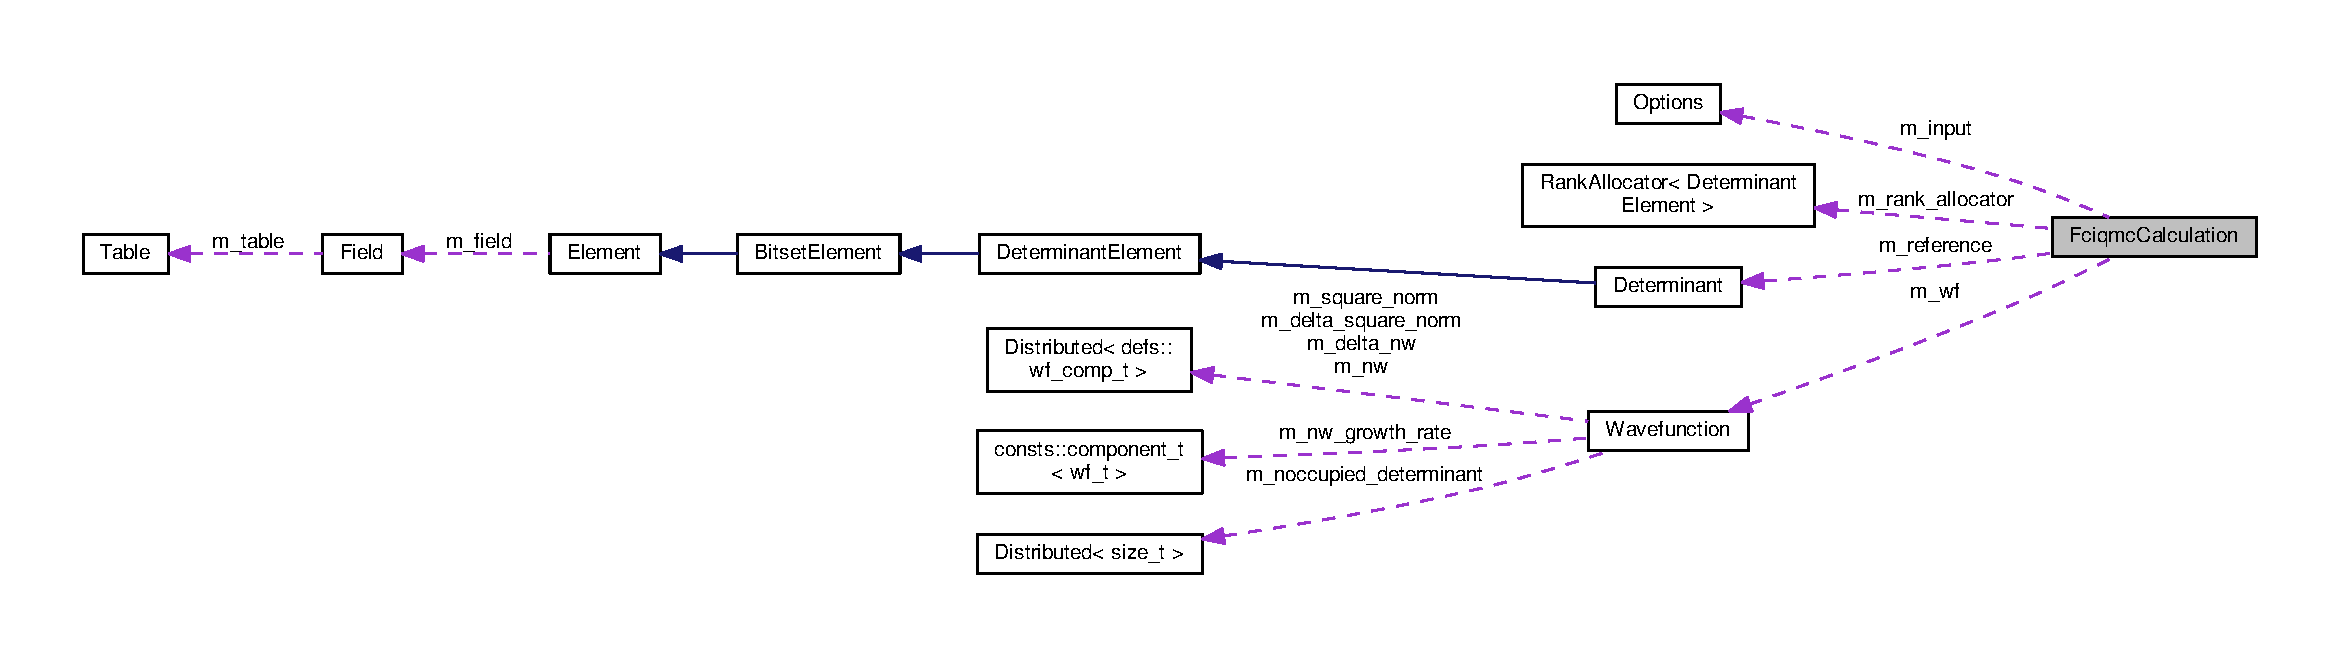
\includegraphics[width=350pt]{classFciqmcCalculation__coll__graph}
\end{center}
\end{figure}
\subsection*{Public Member Functions}
\begin{DoxyCompactItemize}
\item 
{\bfseries Fciqmc\+Calculation} (const \hyperlink{structOptions}{Options} \&input)\hypertarget{classFciqmcCalculation_a7ad3b249a7b10c8a4e199f7b5b1cd3a6}{}\label{classFciqmcCalculation_a7ad3b249a7b10c8a4e199f7b5b1cd3a6}

\item 
void {\bfseries execute} ()\hypertarget{classFciqmcCalculation_a4dd7b05054552de32424ef19221f89db}{}\label{classFciqmcCalculation_a4dd7b05054552de32424ef19221f89db}

\item 
void {\bfseries write\+\_\+iter\+\_\+stats} (size\+\_\+t icycle)\hypertarget{classFciqmcCalculation_ae315657d8686933c407fa66d08997820}{}\label{classFciqmcCalculation_ae315657d8686933c407fa66d08997820}

\end{DoxyCompactItemize}
\subsection*{Public Attributes}
\begin{DoxyCompactItemize}
\item 
const \hyperlink{structOptions}{Options} {\bfseries m\+\_\+input}\hypertarget{classFciqmcCalculation_a6bd0fbd0be08d02508374f210fd697e9}{}\label{classFciqmcCalculation_a6bd0fbd0be08d02508374f210fd697e9}

\item 
\hyperlink{classRankAllocator}{Rank\+Allocator}$<$ \hyperlink{classDeterminantElement}{Determinant\+Element} $>$ {\bfseries m\+\_\+rank\+\_\+allocator}\hypertarget{classFciqmcCalculation_ae436921849704c8c6e506e852cd351b4}{}\label{classFciqmcCalculation_ae436921849704c8c6e506e852cd351b4}

\item 
std\+::unique\+\_\+ptr$<$ \hyperlink{structFciqmcStatsFile}{Fciqmc\+Stats\+File} $>$ {\bfseries m\+\_\+stats\+\_\+file} = nullptr\hypertarget{classFciqmcCalculation_a8ed0b6f6ea5000b28b8b6ac9a94dc9bd}{}\label{classFciqmcCalculation_a8ed0b6f6ea5000b28b8b6ac9a94dc9bd}

\item 
std\+::unique\+\_\+ptr$<$ \hyperlink{classHamiltonian}{Hamiltonian} $>$ {\bfseries m\+\_\+ham}\hypertarget{classFciqmcCalculation_a36f70fc13cb06d9677f1fb99fd5c6fe2}{}\label{classFciqmcCalculation_a36f70fc13cb06d9677f1fb99fd5c6fe2}

\item 
\hyperlink{classDeterminant}{Determinant} {\bfseries m\+\_\+reference}\hypertarget{classFciqmcCalculation_a6d40f0135cd279b0310ffe7d61c3ddbd}{}\label{classFciqmcCalculation_a6d40f0135cd279b0310ffe7d61c3ddbd}

\item 
std\+::unique\+\_\+ptr$<$ \hyperlink{classPropagator}{Propagator} $>$ {\bfseries m\+\_\+prop}\hypertarget{classFciqmcCalculation_aed91e3c62c69624dd60d37309d6ff0f9}{}\label{classFciqmcCalculation_aed91e3c62c69624dd60d37309d6ff0f9}

\item 
\hyperlink{classWavefunction}{Wavefunction} {\bfseries m\+\_\+wf}\hypertarget{classFciqmcCalculation_ac343a139f53dbbc24384633144da4400}{}\label{classFciqmcCalculation_ac343a139f53dbbc24384633144da4400}

\item 
std\+::unique\+\_\+ptr$<$ \hyperlink{structFciqmcScratch}{Fciqmc\+Scratch} $>$ {\bfseries m\+\_\+scratch}\hypertarget{classFciqmcCalculation_a92ef80019a6e28e2d32df3c4bfa3db5d}{}\label{classFciqmcCalculation_a92ef80019a6e28e2d32df3c4bfa3db5d}

\end{DoxyCompactItemize}


The documentation for this class was generated from the following files\+:\begin{DoxyCompactItemize}
\item 
/home/teamcity/\+Team\+City/build\+Agent/work/5343cdffda4690e5/src/core/dynamics/Fciqmc\+Calculation.\+h\item 
/home/teamcity/\+Team\+City/build\+Agent/work/5343cdffda4690e5/src/core/dynamics/Fciqmc\+Calculation.\+cpp\end{DoxyCompactItemize}

\hypertarget{structFciqmcScratch}{}\section{Fciqmc\+Scratch Struct Reference}
\label{structFciqmcScratch}\index{Fciqmc\+Scratch@{Fciqmc\+Scratch}}
\subsection*{Public Member Functions}
\begin{DoxyCompactItemize}
\item 
{\bfseries Fciqmc\+Scratch} (const \hyperlink{classDeterminantElement}{Determinant\+Element} \&ref)\hypertarget{structFciqmcScratch_ab4807f219ec8bfaec979b4e45ac2d50c}{}\label{structFciqmcScratch_ab4807f219ec8bfaec979b4e45ac2d50c}

\end{DoxyCompactItemize}
\subsection*{Public Attributes}
\begin{DoxyCompactItemize}
\item 
std\+::unique\+\_\+ptr$<$ \hyperlink{classPrivateStore}{Private\+Store}$<$ \hyperlink{structOccupiedOrbitals}{Occupied\+Orbitals} $>$ $>$ {\bfseries occ}\hypertarget{structFciqmcScratch_a876ccf9d808da2036399e38b32d7c655}{}\label{structFciqmcScratch_a876ccf9d808da2036399e38b32d7c655}

\item 
std\+::unique\+\_\+ptr$<$ \hyperlink{classPrivateStore}{Private\+Store}$<$ \hyperlink{structVacantOrbitals}{Vacant\+Orbitals} $>$ $>$ {\bfseries vac}\hypertarget{structFciqmcScratch_aa5f60fd17fb49d80dc8817570e5ace5e}{}\label{structFciqmcScratch_aa5f60fd17fb49d80dc8817570e5ace5e}

\item 
std\+::unique\+\_\+ptr$<$ \hyperlink{classPrivateStore}{Private\+Store}$<$ \hyperlink{classConnection}{Connection} $>$ $>$ {\bfseries conn}\hypertarget{structFciqmcScratch_a1d60b2dce20aa3b9d99a5c5a27cdc444}{}\label{structFciqmcScratch_a1d60b2dce20aa3b9d99a5c5a27cdc444}

\item 
std\+::unique\+\_\+ptr$<$ \hyperlink{classPrivateStore}{Private\+Store}$<$ \hyperlink{classAntisymConnection}{Antisym\+Connection} $>$ $>$ {\bfseries anticonn}\hypertarget{structFciqmcScratch_a8450fe8ed94192373d279f8fdf5374ef}{}\label{structFciqmcScratch_a8450fe8ed94192373d279f8fdf5374ef}

\end{DoxyCompactItemize}
\subsection*{Static Public Attributes}
\begin{DoxyCompactItemize}
\item 
static const size\+\_\+t {\bfseries nelement\+\_\+occ}\hypertarget{structFciqmcScratch_a497d061a3f951b688637677c265c5e58}{}\label{structFciqmcScratch_a497d061a3f951b688637677c265c5e58}

\item 
static const size\+\_\+t {\bfseries nelement\+\_\+vac}\hypertarget{structFciqmcScratch_ae2441aed8db6d73b4f978b8730b8ed7c}{}\label{structFciqmcScratch_ae2441aed8db6d73b4f978b8730b8ed7c}

\item 
static const size\+\_\+t {\bfseries nelement\+\_\+conn}\hypertarget{structFciqmcScratch_a9a2f23390205ff070902f000dd9638cb}{}\label{structFciqmcScratch_a9a2f23390205ff070902f000dd9638cb}

\item 
static const size\+\_\+t {\bfseries nelement\+\_\+anticonn}\hypertarget{structFciqmcScratch_ac9ffa7a9991408c31c09c25fb6b5a4eb}{}\label{structFciqmcScratch_ac9ffa7a9991408c31c09c25fb6b5a4eb}

\end{DoxyCompactItemize}


The documentation for this struct was generated from the following files\+:\begin{DoxyCompactItemize}
\item 
/home/teamcity/\+Team\+City/build\+Agent/work/5343cdffda4690e5/src/core/dynamics/Fciqmc\+Scratch.\+h\item 
/home/teamcity/\+Team\+City/build\+Agent/work/5343cdffda4690e5/src/core/dynamics/Fciqmc\+Scratch.\+cpp\end{DoxyCompactItemize}

\hypertarget{structFciqmcStatsFile}{}\doxysection{Fciqmc\+Stats\+File Struct Reference}
\label{structFciqmcStatsFile}\index{FciqmcStatsFile@{FciqmcStatsFile}}


Inheritance diagram for Fciqmc\+Stats\+File\+:\nopagebreak
\begin{figure}[H]
\begin{center}
\leavevmode
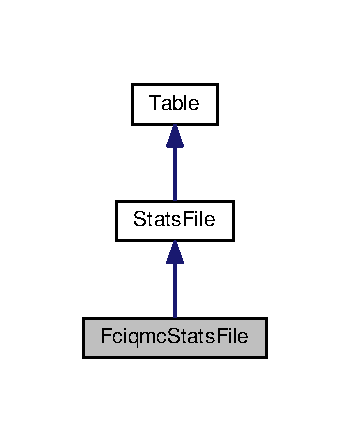
\includegraphics[width=168pt]{structFciqmcStatsFile__inherit__graph}
\end{center}
\end{figure}


Collaboration diagram for Fciqmc\+Stats\+File\+:\nopagebreak
\begin{figure}[H]
\begin{center}
\leavevmode
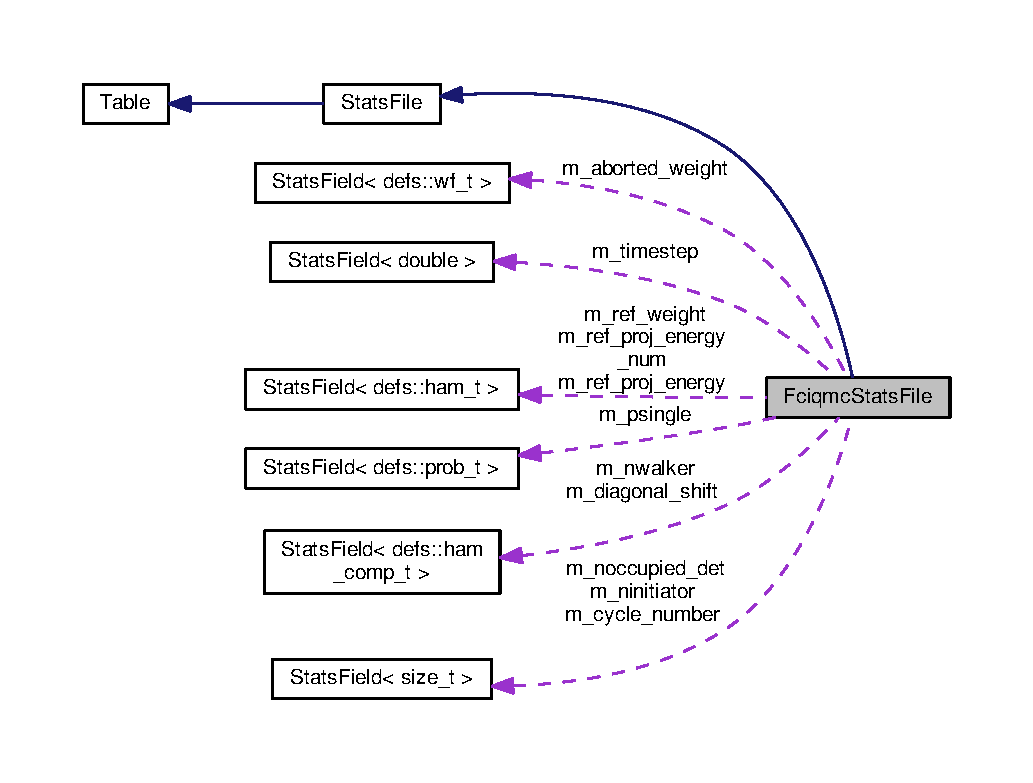
\includegraphics[width=350pt]{structFciqmcStatsFile__coll__graph}
\end{center}
\end{figure}
\doxysubsection*{Public Member Functions}
\begin{DoxyCompactItemize}
\item 
\mbox{\Hypertarget{structFciqmcStatsFile_a077b949e882f2e2d560ef642f2c355bf}\label{structFciqmcStatsFile_a077b949e882f2e2d560ef642f2c355bf}} 
{\bfseries Fciqmc\+Stats\+File} (const \mbox{\hyperlink{structOptions}{Options}} \&input)
\end{DoxyCompactItemize}
\doxysubsection*{Public Attributes}
\begin{DoxyCompactItemize}
\item 
\mbox{\Hypertarget{structFciqmcStatsFile_a0e180ff5c99f2b80c50e7294b2e5b344}\label{structFciqmcStatsFile_a0e180ff5c99f2b80c50e7294b2e5b344}} 
\mbox{\hyperlink{classStatsField}{Stats\+Field}}$<$ size\+\_\+t $>$ {\bfseries m\+\_\+cycle\+\_\+number}
\item 
\mbox{\Hypertarget{structFciqmcStatsFile_abf8839451047afbc3f78de5f9cb799a5}\label{structFciqmcStatsFile_abf8839451047afbc3f78de5f9cb799a5}} 
\mbox{\hyperlink{classStatsField}{Stats\+Field}}$<$ defs\+::ham\+\_\+comp\+\_\+t $>$ {\bfseries m\+\_\+diagonal\+\_\+shift}
\item 
\mbox{\Hypertarget{structFciqmcStatsFile_a72fbd022cf32dcd1b8fe8e711cd91f58}\label{structFciqmcStatsFile_a72fbd022cf32dcd1b8fe8e711cd91f58}} 
\mbox{\hyperlink{classStatsField}{Stats\+Field}}$<$ double $>$ {\bfseries m\+\_\+timestep}
\item 
\mbox{\Hypertarget{structFciqmcStatsFile_a7f879a67c47ae9a82278e7c2b2e44876}\label{structFciqmcStatsFile_a7f879a67c47ae9a82278e7c2b2e44876}} 
\mbox{\hyperlink{classStatsField}{Stats\+Field}}$<$ defs\+::ham\+\_\+t $>$ {\bfseries m\+\_\+ref\+\_\+proj\+\_\+energy\+\_\+num}
\item 
\mbox{\Hypertarget{structFciqmcStatsFile_a90e6c05b9318afa4b5c6199856121342}\label{structFciqmcStatsFile_a90e6c05b9318afa4b5c6199856121342}} 
\mbox{\hyperlink{classStatsField}{Stats\+Field}}$<$ defs\+::ham\+\_\+t $>$ {\bfseries m\+\_\+ref\+\_\+weight}
\item 
\mbox{\Hypertarget{structFciqmcStatsFile_abbb23c945569ceeec15e562b2f933ecd}\label{structFciqmcStatsFile_abbb23c945569ceeec15e562b2f933ecd}} 
\mbox{\hyperlink{classStatsField}{Stats\+Field}}$<$ defs\+::ham\+\_\+t $>$ {\bfseries m\+\_\+ref\+\_\+proj\+\_\+energy}
\item 
\mbox{\Hypertarget{structFciqmcStatsFile_a749a51f565ba3224131003aea8619092}\label{structFciqmcStatsFile_a749a51f565ba3224131003aea8619092}} 
\mbox{\hyperlink{classStatsField}{Stats\+Field}}$<$ defs\+::ham\+\_\+comp\+\_\+t $>$ {\bfseries m\+\_\+nwalker}
\item 
\mbox{\Hypertarget{structFciqmcStatsFile_a12839d801fc75ae7ad1558fa2e56b9c2}\label{structFciqmcStatsFile_a12839d801fc75ae7ad1558fa2e56b9c2}} 
\mbox{\hyperlink{classStatsField}{Stats\+Field}}$<$ size\+\_\+t $>$ {\bfseries m\+\_\+ninitiator}
\item 
\mbox{\Hypertarget{structFciqmcStatsFile_afd1f51baf902f34321c97c10f09fbfc1}\label{structFciqmcStatsFile_afd1f51baf902f34321c97c10f09fbfc1}} 
\mbox{\hyperlink{classStatsField}{Stats\+Field}}$<$ defs\+::wf\+\_\+t $>$ {\bfseries m\+\_\+aborted\+\_\+weight}
\item 
\mbox{\Hypertarget{structFciqmcStatsFile_aba0ef2d54fe7a9ac7dfdf445853abd1c}\label{structFciqmcStatsFile_aba0ef2d54fe7a9ac7dfdf445853abd1c}} 
\mbox{\hyperlink{classStatsField}{Stats\+Field}}$<$ size\+\_\+t $>$ {\bfseries m\+\_\+noccupied\+\_\+det}
\item 
\mbox{\Hypertarget{structFciqmcStatsFile_ac3fa2541af043bd215490f2d4e9cde5a}\label{structFciqmcStatsFile_ac3fa2541af043bd215490f2d4e9cde5a}} 
\mbox{\hyperlink{classStatsField}{Stats\+Field}}$<$ defs\+::prob\+\_\+t $>$ {\bfseries m\+\_\+psingle}
\end{DoxyCompactItemize}
\doxysubsection*{Additional Inherited Members}


The documentation for this struct was generated from the following file\+:\begin{DoxyCompactItemize}
\item 
/home/teamcity/\+Team\+City/build\+Agent/work/5343cdffda4690e5/src/core/io/Fciqmc\+Stats\+File.\+h\end{DoxyCompactItemize}

\hypertarget{classField}{}\section{Field Class Reference}
\label{classField}\index{Field@{Field}}


Inheritance diagram for Field\+:\nopagebreak
\begin{figure}[H]
\begin{center}
\leavevmode
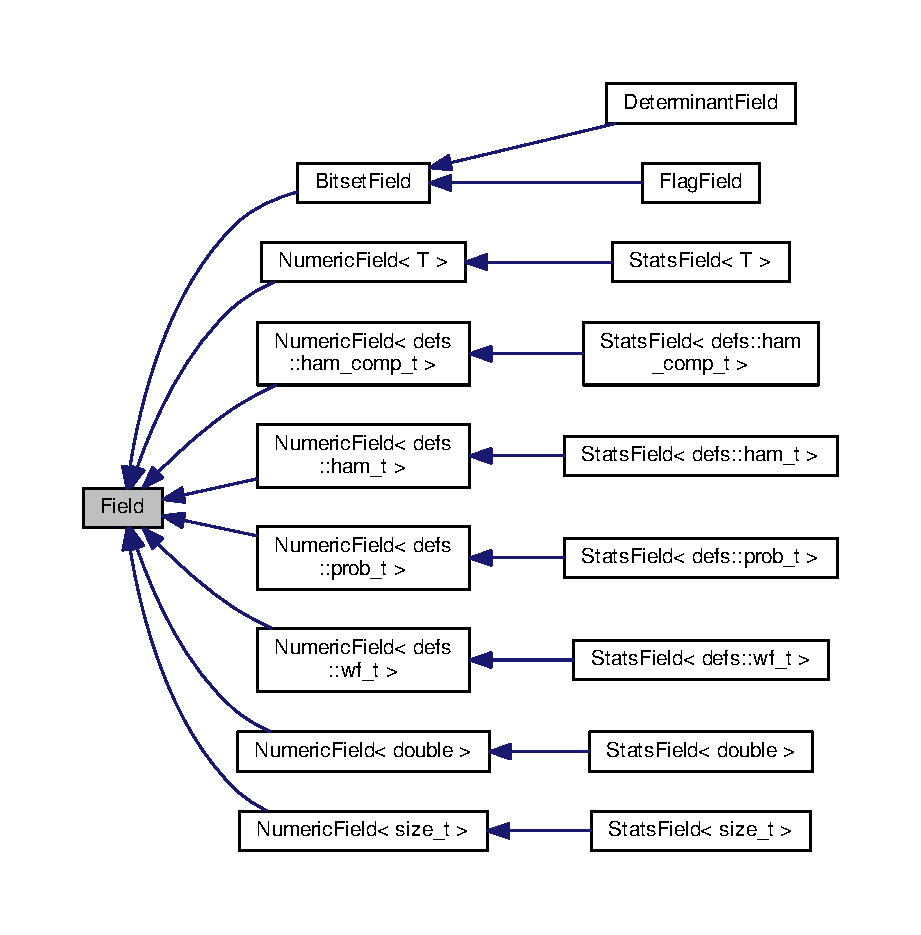
\includegraphics[width=350pt]{classField__inherit__graph}
\end{center}
\end{figure}


Collaboration diagram for Field\+:\nopagebreak
\begin{figure}[H]
\begin{center}
\leavevmode
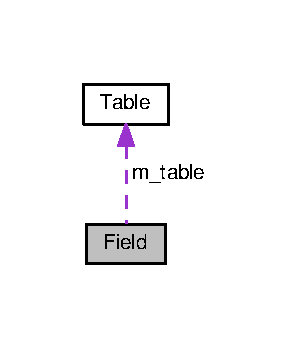
\includegraphics[width=139pt]{classField__coll__graph}
\end{center}
\end{figure}
\subsection*{Public Member Functions}
\begin{DoxyCompactItemize}
\item 
{\bfseries Field} (\hyperlink{classTable}{Table} $\ast$table, size\+\_\+t element\+\_\+size, size\+\_\+t nelement, const std\+::type\+\_\+info \&type\+\_\+info, const std\+::string \&description=\char`\"{}\char`\"{})\hypertarget{classField_a99a8a91be12a04cfbf796655d1bdc43d}{}\label{classField_a99a8a91be12a04cfbf796655d1bdc43d}

\item 
\hyperlink{classElement}{Element} {\bfseries operator()} (const size\+\_\+t \&irow, const size\+\_\+t \&isegment=0, const size\+\_\+t \&ielement=0)\hypertarget{classField_aec27d013e8544087b0aafa457f5c366e}{}\label{classField_aec27d013e8544087b0aafa457f5c366e}

\item 
bool {\bfseries compatible\+\_\+with} (const \hyperlink{classField}{Field} \&rhs) const \hypertarget{classField_aebde47e87596764d7862ed15e4e5985d}{}\label{classField_aebde47e87596764d7862ed15e4e5985d}

\item 
virtual size\+\_\+t {\bfseries nbit} () const \hypertarget{classField_ace43d6bf3c0d9daeda885e6c0341daba}{}\label{classField_ace43d6bf3c0d9daeda885e6c0341daba}

\item 
virtual size\+\_\+t {\bfseries element\+\_\+dsize} () const \hypertarget{classField_a8fd3669ef9680dd50c7d2fb861fbd758}{}\label{classField_a8fd3669ef9680dd50c7d2fb861fbd758}

\item 
virtual bool {\bfseries is\+\_\+complex} () const \hypertarget{classField_ab058d452a9187782ff3d32bbf4155e21}{}\label{classField_ab058d452a9187782ff3d32bbf4155e21}

\item 
virtual const std\+::string {\bfseries description} () const \hypertarget{classField_a08330e74f21963329bbcdd2609b5d77e}{}\label{classField_a08330e74f21963329bbcdd2609b5d77e}

\item 
void {\bfseries expand\+\_\+table} (size\+\_\+t delta\+\_\+nrow)\hypertarget{classField_a8f260d0da4c9c1cb9d3b34dac14379b5}{}\label{classField_a8f260d0da4c9c1cb9d3b34dac14379b5}

\item 
bool {\bfseries is\+\_\+allocated} () const \hypertarget{classField_a9b6c13c9577ce803d03ea56d0b220170}{}\label{classField_a9b6c13c9577ce803d03ea56d0b220170}

\item 
virtual std\+::string {\bfseries to\+\_\+string} (size\+\_\+t irow, size\+\_\+t isegment, size\+\_\+t ielement)\hypertarget{classField_a7027f7704b3dd815171ec0673b015680}{}\label{classField_a7027f7704b3dd815171ec0673b015680}

\item 
void {\bfseries zero} (size\+\_\+t irow, size\+\_\+t isegment=0)\hypertarget{classField_a8f7e5b0d893a09a654c890d5e2723bb3}{}\label{classField_a8f7e5b0d893a09a654c890d5e2723bb3}

\end{DoxyCompactItemize}
\subsection*{Protected Member Functions}
\begin{DoxyCompactItemize}
\item 
char $\ast$ {\bfseries begin} (const size\+\_\+t \&irow, const size\+\_\+t \&isegment=0)\hypertarget{classField_a8402c4cc84e7c2559bb200c0a770a999}{}\label{classField_a8402c4cc84e7c2559bb200c0a770a999}

\item 
char $\ast$ {\bfseries element\+\_\+begin} (const size\+\_\+t \&irow, const size\+\_\+t \&isegment=0, const size\+\_\+t \&ielement=0)\hypertarget{classField_ac744b63e719e32c642d7628e0135f91d}{}\label{classField_ac744b63e719e32c642d7628e0135f91d}

\end{DoxyCompactItemize}
\subsection*{Protected Attributes}
\begin{DoxyCompactItemize}
\item 
\hyperlink{classTable}{Table} $\ast$ {\bfseries m\+\_\+table}\hypertarget{classField_a54a544919cae4a82cc3b0a0f27a9ae83}{}\label{classField_a54a544919cae4a82cc3b0a0f27a9ae83}

\item 
size\+\_\+t {\bfseries m\+\_\+element\+\_\+size}\hypertarget{classField_afb9ba6afceb67426d1c2e701c431d0dc}{}\label{classField_afb9ba6afceb67426d1c2e701c431d0dc}

\item 
size\+\_\+t {\bfseries m\+\_\+element\+\_\+dsize}\hypertarget{classField_a27d0770760813f5575572c321bc5dfb4}{}\label{classField_a27d0770760813f5575572c321bc5dfb4}

\item 
const size\+\_\+t {\bfseries m\+\_\+nelement}\hypertarget{classField_ab75911accbec2a191ca4d3e83ae0d8d6}{}\label{classField_ab75911accbec2a191ca4d3e83ae0d8d6}

\item 
const std\+::type\+\_\+index {\bfseries m\+\_\+type\+\_\+index}\hypertarget{classField_a48aad74f71a6d7e4e433f5f9b3d5f6aa}{}\label{classField_a48aad74f71a6d7e4e433f5f9b3d5f6aa}

\item 
size\+\_\+t {\bfseries m\+\_\+offset}\hypertarget{classField_abae1dcf7cb1039f6742d6eafdf23b410}{}\label{classField_abae1dcf7cb1039f6742d6eafdf23b410}

\item 
std\+::string {\bfseries m\+\_\+description}\hypertarget{classField_aff8011af4412aca320a1ecfc1ae9be1c}{}\label{classField_aff8011af4412aca320a1ecfc1ae9be1c}

\end{DoxyCompactItemize}
\subsection*{Friends}
\begin{DoxyCompactItemize}
\item 
class {\bfseries Table}\hypertarget{classField_af888815e80064bc9fa1035c6265da86e}{}\label{classField_af888815e80064bc9fa1035c6265da86e}

\item 
class {\bfseries Element}\hypertarget{classField_a016b821f88c7c0a2de1451c175cefbf9}{}\label{classField_a016b821f88c7c0a2de1451c175cefbf9}

\end{DoxyCompactItemize}


The documentation for this class was generated from the following files\+:\begin{DoxyCompactItemize}
\item 
/home/teamcity/\+Team\+City/build\+Agent/work/5343cdffda4690e5/src/core/table/Field.\+h\item 
/home/teamcity/\+Team\+City/build\+Agent/work/5343cdffda4690e5/src/core/table/Field.\+cpp\end{DoxyCompactItemize}

\hypertarget{classFileIterator}{}\section{File\+Iterator Class Reference}
\label{classFileIterator}\index{File\+Iterator@{File\+Iterator}}


Inheritance diagram for File\+Iterator\+:\nopagebreak
\begin{figure}[H]
\begin{center}
\leavevmode
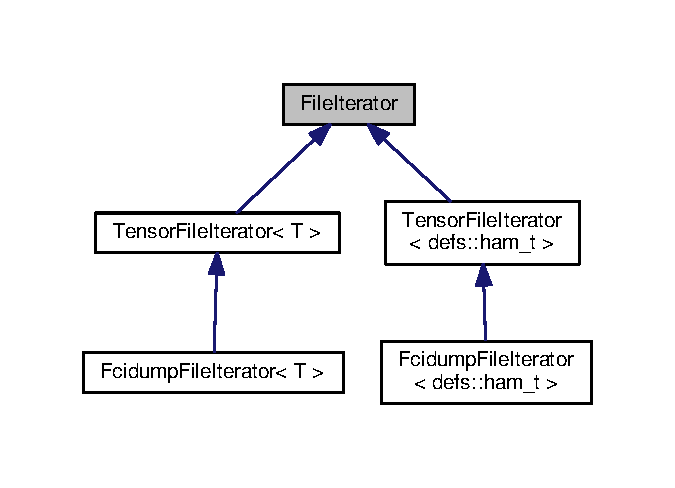
\includegraphics[width=324pt]{classFileIterator__inherit__graph}
\end{center}
\end{figure}
\subsection*{Public Member Functions}
\begin{DoxyCompactItemize}
\item 
{\bfseries File\+Iterator} (const std\+::string \&filename, const size\+\_\+t \&ifirstline)\hypertarget{classFileIterator_a664201608652425655f7631194fc8a5f}{}\label{classFileIterator_a664201608652425655f7631194fc8a5f}

\item 
{\bfseries File\+Iterator} (const std\+::string \&filename)\hypertarget{classFileIterator_a72bdb8a60601e50cc74fa31a3031539e}{}\label{classFileIterator_a72bdb8a60601e50cc74fa31a3031539e}

\item 
{\bfseries File\+Iterator} (const std\+::string \&filename, const std\+::regex \&regex)\hypertarget{classFileIterator_ada8942b79a19dae2a0b668949ac08912}{}\label{classFileIterator_ada8942b79a19dae2a0b668949ac08912}

\item 
bool {\bfseries next} (std\+::string \&)\hypertarget{classFileIterator_a4d395f3fce39962f4a754868143fc318}{}\label{classFileIterator_a4d395f3fce39962f4a754868143fc318}

\item 
std\+::string {\bfseries next} ()\hypertarget{classFileIterator_ad362a010af079bcbfbccdfcc50488b0d}{}\label{classFileIterator_ad362a010af079bcbfbccdfcc50488b0d}

\end{DoxyCompactItemize}
\subsection*{Static Public Member Functions}
\begin{DoxyCompactItemize}
\item 
static const size\+\_\+t {\bfseries line\+\_\+number\+\_\+from\+\_\+regex} (const std\+::string \&, const std\+::regex \&)\hypertarget{classFileIterator_a2e1901e8154e12ea1e103989962b238c}{}\label{classFileIterator_a2e1901e8154e12ea1e103989962b238c}

\end{DoxyCompactItemize}
\subsection*{Protected Attributes}
\begin{DoxyCompactItemize}
\item 
std\+::unique\+\_\+ptr$<$ std\+::ifstream $>$ {\bfseries m\+\_\+file}\hypertarget{classFileIterator_afe5d32129b4d436512b8704062931a53}{}\label{classFileIterator_afe5d32129b4d436512b8704062931a53}

\item 
const size\+\_\+t {\bfseries m\+\_\+ifirstline}\hypertarget{classFileIterator_aa722ca5315390534e9312a796fcbe48b}{}\label{classFileIterator_aa722ca5315390534e9312a796fcbe48b}

\end{DoxyCompactItemize}


The documentation for this class was generated from the following files\+:\begin{DoxyCompactItemize}
\item 
/home/teamcity/\+Team\+City/build\+Agent/work/5343cdffda4690e5/src/core/io/File\+Iterator.\+h\item 
/home/teamcity/\+Team\+City/build\+Agent/work/5343cdffda4690e5/src/core/io/File\+Iterator.\+cpp\end{DoxyCompactItemize}

\hypertarget{classFlag}{}\section{Flag Class Reference}
\label{classFlag}\index{Flag@{Flag}}
\subsection*{Public Member Functions}
\begin{DoxyCompactItemize}
\item 
{\bfseries Flag} (\hyperlink{classFlagField}{Flag\+Field} $\ast$field, size\+\_\+t nelement, const std\+::string \&description=\char`\"{}\char`\"{})\hypertarget{classFlag_ac71458781931b25692e39976794cef5f}{}\label{classFlag_ac71458781931b25692e39976794cef5f}

\item 
\hyperlink{classFlagElement}{Flag\+Element} {\bfseries operator()} (const size\+\_\+t \&irow, const size\+\_\+t \&isegment=0)\hypertarget{classFlag_adbaa4f7306e34de940aa6177e3ef62de}{}\label{classFlag_adbaa4f7306e34de940aa6177e3ef62de}

\item 
const defs\+::pair \& {\bfseries offset} () const \hypertarget{classFlag_aa0df9fa3439c2cde0b35154b5d879de8}{}\label{classFlag_aa0df9fa3439c2cde0b35154b5d879de8}

\end{DoxyCompactItemize}
\subsection*{Friends}
\begin{DoxyCompactItemize}
\item 
class {\bfseries Flag\+Field}\hypertarget{classFlag_a955858e82156003d22c485ab29f79032}{}\label{classFlag_a955858e82156003d22c485ab29f79032}

\end{DoxyCompactItemize}


The documentation for this class was generated from the following files\+:\begin{DoxyCompactItemize}
\item 
/home/teamcity/\+Team\+City/build\+Agent/work/5343cdffda4690e5/src/core/table/Flag.\+h\item 
/home/teamcity/\+Team\+City/build\+Agent/work/5343cdffda4690e5/src/core/table/Flag.\+cpp\end{DoxyCompactItemize}

\hypertarget{classFlagElement}{}\section{Flag\+Element Class Reference}
\label{classFlagElement}\index{Flag\+Element@{Flag\+Element}}
\subsection*{Public Member Functions}
\begin{DoxyCompactItemize}
\item 
{\bfseries Flag\+Element} (\hyperlink{classFlag}{Flag} $\ast$flag, \hyperlink{classBitsetElement}{Bitset\+Element} bitset\+\_\+element)\hypertarget{classFlagElement_a710b228c975dcb93fb442b0cd3a2575f}{}\label{classFlagElement_a710b228c975dcb93fb442b0cd3a2575f}

\item 
void {\bfseries operator=} (bool v)\hypertarget{classFlagElement_a612f90ed54bd4b0f96472ce1478eaada}{}\label{classFlagElement_a612f90ed54bd4b0f96472ce1478eaada}

\item 
{\bfseries operator bool} ()\hypertarget{classFlagElement_a6335fd27d53907333b016e802e9bbbc9}{}\label{classFlagElement_a6335fd27d53907333b016e802e9bbbc9}

\end{DoxyCompactItemize}


The documentation for this class was generated from the following files\+:\begin{DoxyCompactItemize}
\item 
/home/teamcity/\+Team\+City/build\+Agent/work/5343cdffda4690e5/src/core/table/Flag.\+h\item 
/home/teamcity/\+Team\+City/build\+Agent/work/5343cdffda4690e5/src/core/table/Flag.\+cpp\end{DoxyCompactItemize}

\hypertarget{classFlagField}{}\section{Flag\+Field Class Reference}
\label{classFlagField}\index{Flag\+Field@{Flag\+Field}}


Inheritance diagram for Flag\+Field\+:
% FIG 0


Collaboration diagram for Flag\+Field\+:
% FIG 1
\subsection*{Public Member Functions}
\begin{DoxyCompactItemize}
\item 
{\bfseries Flag\+Field} (\hyperlink{classTable}{Table} $\ast$table, size\+\_\+t nelement, const std\+::string \&description)\hypertarget{classFlagField_af1cf5752d23bee71cad1e8f9e5c0d90c}{}\label{classFlagField_af1cf5752d23bee71cad1e8f9e5c0d90c}

\item 
defs\+::pair {\bfseries add\+\_\+flag} (\hyperlink{classFlag}{Flag} $\ast$flag)\hypertarget{classFlagField_a288b67beb33841ecdb06f3af772682d1}{}\label{classFlagField_a288b67beb33841ecdb06f3af772682d1}

\item 
const std\+::string {\bfseries description} () const override\hypertarget{classFlagField_adba81577f60c7b80923394a5437234fa}{}\label{classFlagField_adba81577f60c7b80923394a5437234fa}

\end{DoxyCompactItemize}
\subsection*{Friends}
\begin{DoxyCompactItemize}
\item 
class {\bfseries Flag}\hypertarget{classFlagField_a3c61b282d6d35a5f37ea21d544b6a633}{}\label{classFlagField_a3c61b282d6d35a5f37ea21d544b6a633}

\end{DoxyCompactItemize}
\subsection*{Additional Inherited Members}


The documentation for this class was generated from the following files\+:\begin{DoxyCompactItemize}
\item 
/home/teamcity/\+Team\+City/build\+Agent/work/5343cdffda4690e5/src/core/table/Flag\+Field.\+h\item 
/home/teamcity/\+Team\+City/build\+Agent/work/5343cdffda4690e5/src/core/table/Flag\+Field.\+cpp\end{DoxyCompactItemize}

\hypertarget{classHamiltonian}{}\doxysection{Hamiltonian Class Reference}
\label{classHamiltonian}\index{Hamiltonian@{Hamiltonian}}


Inheritance diagram for Hamiltonian\+:\nopagebreak
\begin{figure}[H]
\begin{center}
\leavevmode
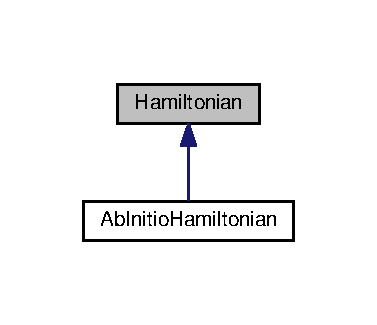
\includegraphics[width=181pt]{classHamiltonian__inherit__graph}
\end{center}
\end{figure}
\doxysubsection*{Classes}
\begin{DoxyCompactItemize}
\item 
class \mbox{\hyperlink{classHamiltonian_1_1ConnectionList}{Connection\+List}}
\item 
class \mbox{\hyperlink{classHamiltonian_1_1DeterminantList}{Determinant\+List}}
\end{DoxyCompactItemize}
\doxysubsection*{Public Member Functions}
\begin{DoxyCompactItemize}
\item 
\mbox{\Hypertarget{classHamiltonian_aea9fe1aef1bf9bd4799a2b957c550f02}\label{classHamiltonian_aea9fe1aef1bf9bd4799a2b957c550f02}} 
{\bfseries Hamiltonian} (const size\+\_\+t \&nsite)
\item 
\mbox{\Hypertarget{classHamiltonian_a8e7844e3fe02b9cd9de556c7fc7454ac}\label{classHamiltonian_a8e7844e3fe02b9cd9de556c7fc7454ac}} 
\mbox{\hyperlink{structconsts_1_1component__t}{consts\+::component\+\_\+t}}$<$ defs\+::ham\+\_\+t $>$\+::type {\bfseries get\+\_\+energy} (const \mbox{\hyperlink{classDeterminantElement}{Determinant\+Element}} \&det) const
\item 
\mbox{\Hypertarget{classHamiltonian_a1042c841212b35ea08b0714942134dec}\label{classHamiltonian_a1042c841212b35ea08b0714942134dec}} 
virtual defs\+::ham\+\_\+t {\bfseries get\+\_\+element\+\_\+0} (const defs\+::det\+\_\+work \&occs, const size\+\_\+t \&nocc) const =0
\item 
\mbox{\Hypertarget{classHamiltonian_a8944945ff8fe0ba62d39b0dfbe75ece6}\label{classHamiltonian_a8944945ff8fe0ba62d39b0dfbe75ece6}} 
defs\+::ham\+\_\+t {\bfseries get\+\_\+element\+\_\+0} (const \mbox{\hyperlink{structOccupiedOrbitals}{Occupied\+Orbitals}} \&occs) const
\item 
\mbox{\Hypertarget{classHamiltonian_aaf20ea0c5334bf7ff6248b888508856c}\label{classHamiltonian_aaf20ea0c5334bf7ff6248b888508856c}} 
defs\+::ham\+\_\+t {\bfseries get\+\_\+element\+\_\+0} (const \mbox{\hyperlink{classDeterminantElement}{Determinant\+Element}} \&det) const
\item 
\mbox{\Hypertarget{classHamiltonian_a829e544ae21fdd48056194a3d728a028}\label{classHamiltonian_a829e544ae21fdd48056194a3d728a028}} 
defs\+::ham\+\_\+t {\bfseries get\+\_\+element\+\_\+0} (const \mbox{\hyperlink{classAntisymConnection}{Antisym\+Connection}} \&connection) const
\item 
\mbox{\Hypertarget{classHamiltonian_aa1d2b517a085e7fb0488bc2874f075fe}\label{classHamiltonian_aa1d2b517a085e7fb0488bc2874f075fe}} 
virtual defs\+::ham\+\_\+t {\bfseries get\+\_\+element\+\_\+1} (const \mbox{\hyperlink{classAntisymConnection}{Antisym\+Connection}} \&connection) const =0
\item 
\mbox{\Hypertarget{classHamiltonian_a85cb450f38fb23fcf415c6799c1a661f}\label{classHamiltonian_a85cb450f38fb23fcf415c6799c1a661f}} 
virtual defs\+::ham\+\_\+t {\bfseries get\+\_\+element\+\_\+2} (const size\+\_\+t \&i, const size\+\_\+t \&j, const size\+\_\+t \&k, const size\+\_\+t \&l) const =0
\item 
\mbox{\Hypertarget{classHamiltonian_a82271a080e62d9a6b48dca4dec4d2e6c}\label{classHamiltonian_a82271a080e62d9a6b48dca4dec4d2e6c}} 
defs\+::ham\+\_\+t {\bfseries get\+\_\+element\+\_\+2} (const \mbox{\hyperlink{classConnection}{Connection}} \&connection) const
\item 
\mbox{\Hypertarget{classHamiltonian_a2c098a580ab7260fc092e4a8d5021e70}\label{classHamiltonian_a2c098a580ab7260fc092e4a8d5021e70}} 
defs\+::ham\+\_\+t {\bfseries get\+\_\+element\+\_\+2} (const \mbox{\hyperlink{classAntisymConnection}{Antisym\+Connection}} \&connection) const
\item 
\mbox{\Hypertarget{classHamiltonian_a1dfe25006968ef99aa318679d49f8f15}\label{classHamiltonian_a1dfe25006968ef99aa318679d49f8f15}} 
defs\+::ham\+\_\+t {\bfseries get\+\_\+element} (const \mbox{\hyperlink{classAntisymConnection}{Antisym\+Connection}} \&connection) const
\item 
\mbox{\Hypertarget{classHamiltonian_ae6562e780d8d2826287a1491871c797a}\label{classHamiltonian_ae6562e780d8d2826287a1491871c797a}} 
defs\+::ham\+\_\+t {\bfseries get\+\_\+element} (const \mbox{\hyperlink{classDeterminantElement}{Determinant\+Element}} \&bra, const \mbox{\hyperlink{classDeterminantElement}{Determinant\+Element}} \&ket) const
\item 
\mbox{\Hypertarget{classHamiltonian_ab3a853495ae70b38d05cbcd486b4bfe2}\label{classHamiltonian_ab3a853495ae70b38d05cbcd486b4bfe2}} 
size\+\_\+t {\bfseries nsite} () const
\item 
\mbox{\Hypertarget{classHamiltonian_ac2b50f89de2d63399a0d6b98a66b27a8}\label{classHamiltonian_ac2b50f89de2d63399a0d6b98a66b27a8}} 
size\+\_\+t {\bfseries nci} () const
\item 
\mbox{\Hypertarget{classHamiltonian_ac74a988992ec2108d1fd0ef4455c810c}\label{classHamiltonian_ac74a988992ec2108d1fd0ef4455c810c}} 
virtual bool {\bfseries spin\+\_\+conserving} () const =0
\item 
\mbox{\Hypertarget{classHamiltonian_a6fad47832ce13f6b36232f4c653aa04f}\label{classHamiltonian_a6fad47832ce13f6b36232f4c653aa04f}} 
virtual size\+\_\+t {\bfseries nelec} () const =0
\item 
\mbox{\Hypertarget{classHamiltonian_a0499e9bce6f7adacce98cef9c0d124b1}\label{classHamiltonian_a0499e9bce6f7adacce98cef9c0d124b1}} 
virtual bool {\bfseries spin\+\_\+resolved} () const =0
\item 
\mbox{\Hypertarget{classHamiltonian_a017c819e5b9ac386f2ff3fa6b3926a04}\label{classHamiltonian_a017c819e5b9ac386f2ff3fa6b3926a04}} 
\mbox{\hyperlink{classDeterminant}{Determinant}} {\bfseries guess\+\_\+reference} (const int \&spin\+\_\+level) const
\item 
\mbox{\Hypertarget{classHamiltonian_afe517a3615de41b3520f9941a8821fab}\label{classHamiltonian_afe517a3615de41b3520f9941a8821fab}} 
\mbox{\hyperlink{classDeterminant}{Determinant}} {\bfseries refine\+\_\+guess\+\_\+reference} (const \mbox{\hyperlink{classDeterminantElement}{Determinant\+Element}} \&ref) const
\item 
\mbox{\Hypertarget{classHamiltonian_a9d38784496ffebc1b0fff5afa680eadc}\label{classHamiltonian_a9d38784496ffebc1b0fff5afa680eadc}} 
\mbox{\hyperlink{classDeterminant}{Determinant}} {\bfseries choose\+\_\+reference} (const int \&spin\+\_\+level) const
\item 
\mbox{\Hypertarget{classHamiltonian_ad0276e3f11eae785ec7268f8e7acc7e2}\label{classHamiltonian_ad0276e3f11eae785ec7268f8e7acc7e2}} 
void {\bfseries all\+\_\+connections\+\_\+of\+\_\+det} (\mbox{\hyperlink{classHamiltonian_1_1ConnectionList}{Connection\+List}} $\ast$list, const \mbox{\hyperlink{classDeterminant}{Determinant}} \&ref, const defs\+::ham\+\_\+comp\+\_\+t eps) const
\item 
\mbox{\Hypertarget{classHamiltonian_a0c384e989c90c9a6fcbccb93ca497d42}\label{classHamiltonian_a0c384e989c90c9a6fcbccb93ca497d42}} 
void {\bfseries generate\+\_\+ci\+\_\+space} (\mbox{\hyperlink{structWalkerList}{Walker\+List}} $\ast$list, \mbox{\hyperlink{classRankAllocator}{Rank\+Allocator}}$<$ \mbox{\hyperlink{classDeterminantElement}{Determinant\+Element}} $>$ \&ra, const int \&spin\+\_\+level) const
\end{DoxyCompactItemize}
\doxysubsection*{Protected Attributes}
\begin{DoxyCompactItemize}
\item 
\mbox{\Hypertarget{classHamiltonian_aec7c649696cbf62851f23d081fcb1e8d}\label{classHamiltonian_aec7c649696cbf62851f23d081fcb1e8d}} 
const size\+\_\+t {\bfseries m\+\_\+nsite}
\end{DoxyCompactItemize}


The documentation for this class was generated from the following files\+:\begin{DoxyCompactItemize}
\item 
/home/teamcity/\+Team\+City/build\+Agent/work/5343cdffda4690e5/src/core/hamiltonian/Hamiltonian.\+h\item 
/home/teamcity/\+Team\+City/build\+Agent/work/5343cdffda4690e5/src/core/hamiltonian/Hamiltonian.\+cpp\end{DoxyCompactItemize}

\hypertarget{classHashMap}{}\section{Hash\+Map$<$ T $>$ Class Template Reference}
\label{classHashMap}\index{Hash\+Map$<$ T $>$@{Hash\+Map$<$ T $>$}}


Inheritance diagram for Hash\+Map$<$ T $>$\+:
% FIG 0
\subsection*{Public Member Functions}
\begin{DoxyCompactItemize}
\item 
{\bfseries Hash\+Map} (const size\+\_\+t \&nbucket)\hypertarget{classHashMap_ad3da0496d0d5c817818cc3d0de1cde13}{}\label{classHashMap_ad3da0496d0d5c817818cc3d0de1cde13}

\item 
{\bfseries Hash\+Map} (const \hyperlink{classHashMap}{Hash\+Map} \&old, const size\+\_\+t \&nbucket)\hypertarget{classHashMap_ad084f78eb6a7208b9cc67020703ff898}{}\label{classHashMap_ad084f78eb6a7208b9cc67020703ff898}

\item 
virtual T {\bfseries get\+\_\+key} (const size\+\_\+t \&key\+\_\+index) const =0\hypertarget{classHashMap_a6449e282ff3ee559f254f4f727e9cf63}{}\label{classHashMap_a6449e282ff3ee559f254f4f727e9cf63}

\item 
virtual void {\bfseries set\+\_\+key} (const size\+\_\+t \&key\+\_\+index, const T \&key)=0\hypertarget{classHashMap_a21b01a2502b7f45dd939bab7a3811a54}{}\label{classHashMap_a21b01a2502b7f45dd939bab7a3811a54}

\item 
size\+\_\+t {\bfseries bucket} (const T \&key) const \hypertarget{classHashMap_a36df7df6b87258c2817865583569199b}{}\label{classHashMap_a36df7df6b87258c2817865583569199b}

\item 
virtual size\+\_\+t {\bfseries lookup} (const size\+\_\+t \&ibucket, const T \&key) const \hypertarget{classHashMap_a2e14b85d148e08c85f20eabfa978c185}{}\label{classHashMap_a2e14b85d148e08c85f20eabfa978c185}

\item 
virtual size\+\_\+t {\bfseries lookup} (const T \&key) const \hypertarget{classHashMap_ac4ab5ba76fcb4436e9ccdad3c7790567}{}\label{classHashMap_ac4ab5ba76fcb4436e9ccdad3c7790567}

\item 
virtual void {\bfseries insert} (const size\+\_\+t \&ibucket, const T \&key, const size\+\_\+t \&key\+\_\+index)\hypertarget{classHashMap_aab21199d4692865f989168a2bf02b7e9}{}\label{classHashMap_aab21199d4692865f989168a2bf02b7e9}

\item 
virtual void {\bfseries insert} (const T \&key, const size\+\_\+t \&key\+\_\+index)\hypertarget{classHashMap_a2e75f0e3ffc44c9b4d5821e36756395a}{}\label{classHashMap_a2e75f0e3ffc44c9b4d5821e36756395a}

\item 
virtual size\+\_\+t {\bfseries remove} (const size\+\_\+t \&ibucket, const size\+\_\+t \&key\+\_\+index)\hypertarget{classHashMap_aeb1bfd294550522d4b99cb1fc5855981}{}\label{classHashMap_aeb1bfd294550522d4b99cb1fc5855981}

\item 
virtual size\+\_\+t {\bfseries remove} (const T \&key)\hypertarget{classHashMap_a37060379e724337f2b42cf185f34fdc9}{}\label{classHashMap_a37060379e724337f2b42cf185f34fdc9}

\item 
size\+\_\+t {\bfseries size} () const \hypertarget{classHashMap_a0649c3b72405bfef706d98e281df4bf7}{}\label{classHashMap_a0649c3b72405bfef706d98e281df4bf7}

\item 
bool {\bfseries operator==} (const \hyperlink{classHashMap}{Hash\+Map} \&other) const \hypertarget{classHashMap_a7601c385de515579179c5ad40b2f5865}{}\label{classHashMap_a7601c385de515579179c5ad40b2f5865}

\item 
void {\bfseries print} () const \hypertarget{classHashMap_a805dc87c2829ce7b657ced9f0fa0f958}{}\label{classHashMap_a805dc87c2829ce7b657ced9f0fa0f958}

\end{DoxyCompactItemize}
\subsection*{Protected Attributes}
\begin{DoxyCompactItemize}
\item 
std\+::vector$<$ std\+::forward\+\_\+list$<$ size\+\_\+t $>$ $>$ {\bfseries m\+\_\+buckets}\hypertarget{classHashMap_a962a721172bfc7ec504c756e906b3af4}{}\label{classHashMap_a962a721172bfc7ec504c756e906b3af4}

\end{DoxyCompactItemize}


The documentation for this class was generated from the following file\+:\begin{DoxyCompactItemize}
\item 
/home/teamcity/\+Team\+City/build\+Agent/work/5343cdffda4690e5/src/core/hash/Hash\+Map.\+h\end{DoxyCompactItemize}

\hypertarget{classHeatBathSampler}{}\doxysection{Heat\+Bath\+Sampler Class Reference}
\label{classHeatBathSampler}\index{HeatBathSampler@{HeatBathSampler}}


Collaboration diagram for Heat\+Bath\+Sampler\+:\nopagebreak
\begin{figure}[H]
\begin{center}
\leavevmode
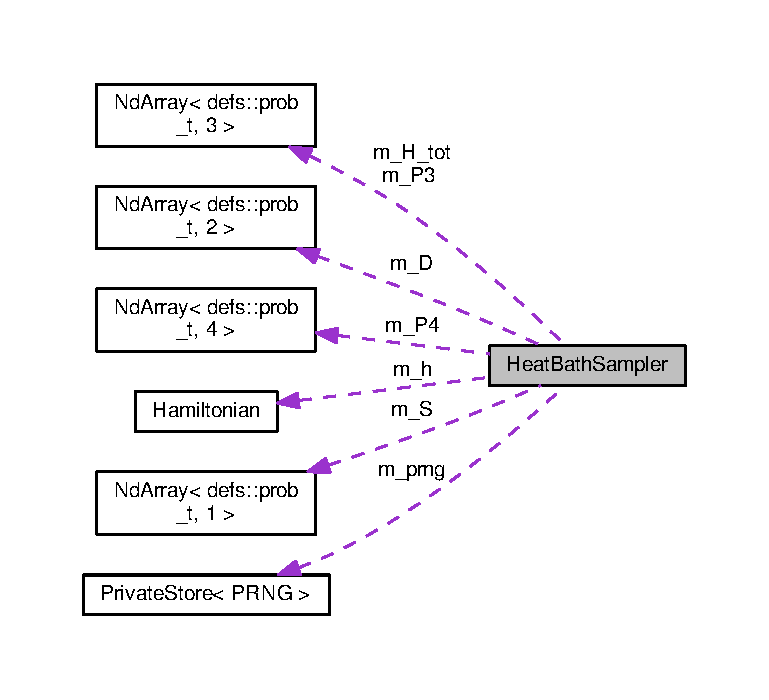
\includegraphics[width=350pt]{classHeatBathSampler__coll__graph}
\end{center}
\end{figure}
\doxysubsection*{Public Member Functions}
\begin{DoxyCompactItemize}
\item 
\mbox{\Hypertarget{classHeatBathSampler_a1451ee391a7bf45458d1200a23cb7ec4}\label{classHeatBathSampler_a1451ee391a7bf45458d1200a23cb7ec4}} 
{\bfseries Heat\+Bath\+Sampler} (const \mbox{\hyperlink{classHamiltonian}{Hamiltonian}} $\ast$m\+\_\+h, \mbox{\hyperlink{classPrivateStore}{Private\+Store}}$<$ \mbox{\hyperlink{classPRNG}{P\+R\+NG}} $>$ \&prng)
\end{DoxyCompactItemize}
\doxysubsection*{Public Attributes}
\begin{DoxyCompactItemize}
\item 
\mbox{\Hypertarget{classHeatBathSampler_a9feb97a6236c0396863bf3033785c6fa}\label{classHeatBathSampler_a9feb97a6236c0396863bf3033785c6fa}} 
const \mbox{\hyperlink{classHamiltonian}{Hamiltonian}} $\ast$ {\bfseries m\+\_\+h}
\item 
\mbox{\Hypertarget{classHeatBathSampler_aac2d2e3f13e8193d507ebcd491b4f44a}\label{classHeatBathSampler_aac2d2e3f13e8193d507ebcd491b4f44a}} 
\mbox{\hyperlink{classPrivateStore}{Private\+Store}}$<$ \mbox{\hyperlink{classPRNG}{P\+R\+NG}} $>$ \& {\bfseries m\+\_\+prng}
\item 
\mbox{\Hypertarget{classHeatBathSampler_a7b3f6c7339b6b02cbce19f71ac798e6e}\label{classHeatBathSampler_a7b3f6c7339b6b02cbce19f71ac798e6e}} 
const size\+\_\+t {\bfseries m\+\_\+nbit}
\item 
\mbox{\Hypertarget{classHeatBathSampler_a06e2bace728f8f540f2698053d363e75}\label{classHeatBathSampler_a06e2bace728f8f540f2698053d363e75}} 
const bool {\bfseries m\+\_\+spin\+\_\+conserving}
\item 
\mbox{\Hypertarget{classHeatBathSampler_a537dec2d0390d75eede2132fff9f67da}\label{classHeatBathSampler_a537dec2d0390d75eede2132fff9f67da}} 
\mbox{\hyperlink{classNdArray}{Nd\+Array}}$<$ defs\+::prob\+\_\+t, 2 $>$ {\bfseries m\+\_\+D}
\item 
\mbox{\Hypertarget{classHeatBathSampler_aba54811d98e2da7b7199ae262015167b}\label{classHeatBathSampler_aba54811d98e2da7b7199ae262015167b}} 
\mbox{\hyperlink{classNdArray}{Nd\+Array}}$<$ defs\+::prob\+\_\+t, 1 $>$ {\bfseries m\+\_\+S}
\item 
\mbox{\Hypertarget{classHeatBathSampler_a5e69f450cf6034420ff174ae2b656ba9}\label{classHeatBathSampler_a5e69f450cf6034420ff174ae2b656ba9}} 
\mbox{\hyperlink{classNdArray}{Nd\+Array}}$<$ defs\+::prob\+\_\+t, 3 $>$ {\bfseries m\+\_\+\+P3}
\item 
\mbox{\Hypertarget{classHeatBathSampler_a197eb4103e8bde4143fe5ce8529c8b9c}\label{classHeatBathSampler_a197eb4103e8bde4143fe5ce8529c8b9c}} 
\mbox{\hyperlink{classNdArray}{Nd\+Array}}$<$ defs\+::prob\+\_\+t, 3 $>$ {\bfseries m\+\_\+\+H\+\_\+tot}
\item 
\mbox{\Hypertarget{classHeatBathSampler_a0cab2d919f0926823d6c3c77ee254d82}\label{classHeatBathSampler_a0cab2d919f0926823d6c3c77ee254d82}} 
\mbox{\hyperlink{classNdArray}{Nd\+Array}}$<$ defs\+::prob\+\_\+t, 4 $>$ {\bfseries m\+\_\+\+P4}
\item 
\mbox{\Hypertarget{classHeatBathSampler_a2dbaa680562054cca20fa8419c4f6228}\label{classHeatBathSampler_a2dbaa680562054cca20fa8419c4f6228}} 
std\+::unique\+\_\+ptr$<$ \mbox{\hyperlink{classPrivateStore}{Private\+Store}}$<$ \mbox{\hyperlink{classDeterminantSampler}{Determinant\+Sampler}} $>$ $>$ {\bfseries det\+\_\+sampler}
\end{DoxyCompactItemize}
\doxysubsection*{Static Public Attributes}
\begin{DoxyCompactItemize}
\item 
\mbox{\Hypertarget{classHeatBathSampler_a9a1765224abde57098fccffb48136860}\label{classHeatBathSampler_a9a1765224abde57098fccffb48136860}} 
static const size\+\_\+t {\bfseries nelement\+\_\+det\+\_\+sampler} = 1
\end{DoxyCompactItemize}


The documentation for this class was generated from the following files\+:\begin{DoxyCompactItemize}
\item 
/home/teamcity/\+Team\+City/build\+Agent/work/5343cdffda4690e5/src/core/heatbath/Heat\+Bath\+Sampler.\+h\item 
/home/teamcity/\+Team\+City/build\+Agent/work/5343cdffda4690e5/src/core/heatbath/Heat\+Bath\+Sampler.\+cpp\end{DoxyCompactItemize}

\hypertarget{classHeatBathSamplers}{}\section{Heat\+Bath\+Samplers Class Reference}
\label{classHeatBathSamplers}\index{Heat\+Bath\+Samplers@{Heat\+Bath\+Samplers}}


Inheritance diagram for Heat\+Bath\+Samplers\+:
\nopagebreak
\begin{figure}[H]
\begin{center}
\leavevmode
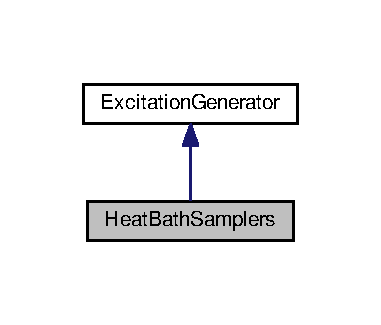
\includegraphics[width=183pt]{classHeatBathSamplers__inherit__graph}
\end{center}
\end{figure}


Collaboration diagram for Heat\+Bath\+Samplers\+:
\nopagebreak
\begin{figure}[H]
\begin{center}
\leavevmode
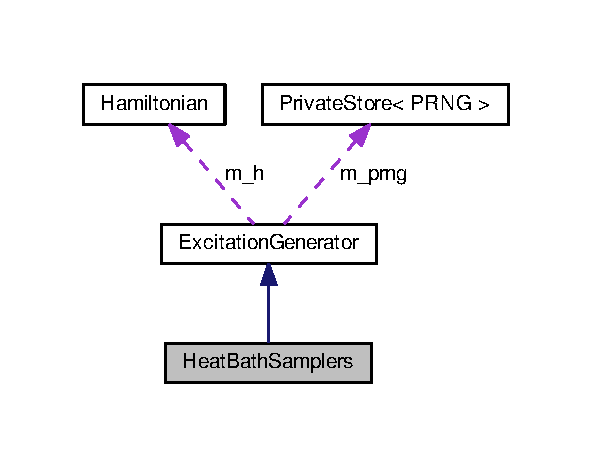
\includegraphics[width=284pt]{classHeatBathSamplers__coll__graph}
\end{center}
\end{figure}
\subsection*{Public Member Functions}
\begin{DoxyCompactItemize}
\item 
{\bfseries Heat\+Bath\+Samplers} (const \hyperlink{classHamiltonian}{Hamiltonian} $\ast$h, \hyperlink{classPrivateStore}{Private\+Store}$<$ \hyperlink{classPRNG}{P\+R\+NG} $>$ \&prng)\hypertarget{classHeatBathSamplers_a6c301f6338de8229f2eb073d7e5fcf0d}{}\label{classHeatBathSamplers_a6c301f6338de8229f2eb073d7e5fcf0d}

\item 
bool {\bfseries draw\+\_\+single} (const \hyperlink{classDeterminantElement}{Determinant\+Element} \&src\+\_\+det, \hyperlink{classDeterminantElement}{Determinant\+Element} \&dst\+\_\+det, const \hyperlink{structOccupiedOrbitals}{Occupied\+Orbitals} \&occ, const \hyperlink{structVacantOrbitals}{Vacant\+Orbitals} \&vac, defs\+::prob\+\_\+t \&prob, defs\+::ham\+\_\+t \&helem, \hyperlink{classAntisymConnection}{Antisym\+Connection} \&anticonn) override\hypertarget{classHeatBathSamplers_a23a35dd94e61b5c6440f54cee19a9fff}{}\label{classHeatBathSamplers_a23a35dd94e61b5c6440f54cee19a9fff}

\item 
bool {\bfseries draw\+\_\+double} (const \hyperlink{classDeterminantElement}{Determinant\+Element} \&src\+\_\+det, \hyperlink{classDeterminantElement}{Determinant\+Element} \&dst\+\_\+det, const \hyperlink{structOccupiedOrbitals}{Occupied\+Orbitals} \&occ, defs\+::prob\+\_\+t \&prob, defs\+::ham\+\_\+t \&helem, \hyperlink{classAntisymConnection}{Antisym\+Connection} \&anticonn) override\hypertarget{classHeatBathSamplers_af8e17179f6ccdee991df488f29234b7c}{}\label{classHeatBathSamplers_af8e17179f6ccdee991df488f29234b7c}

\end{DoxyCompactItemize}
\subsection*{Additional Inherited Members}


The documentation for this class was generated from the following files\+:\begin{DoxyCompactItemize}
\item 
/home/teamcity/\+Team\+City/build\+Agent/work/5343cdffda4690e5/src/core/pchb/Heat\+Bath\+Samplers.\+h\item 
/home/teamcity/\+Team\+City/build\+Agent/work/5343cdffda4690e5/src/core/pchb/Heat\+Bath\+Samplers.\+cpp\end{DoxyCompactItemize}

\hypertarget{classIndexer}{}\doxysection{Indexer$<$ nind $>$ Class Template Reference}
\label{classIndexer}\index{Indexer$<$ nind $>$@{Indexer$<$ nind $>$}}
\doxysubsection*{Public Member Functions}
\begin{DoxyCompactItemize}
\item 
\mbox{\Hypertarget{classIndexer_ae026337e9dc43c757f72965ee7975a59}\label{classIndexer_ae026337e9dc43c757f72965ee7975a59}} 
{\footnotesize template$<$typename ... Args$>$ }\\{\bfseries Indexer} (const size\+\_\+t \&first, Args ...shape)
\item 
\mbox{\Hypertarget{classIndexer_a577b3db95c7010f954e251fb98f1ada2}\label{classIndexer_a577b3db95c7010f954e251fb98f1ada2}} 
{\bfseries Indexer} (const std\+::array$<$ size\+\_\+t, nind $>$ \&shape)
\item 
\mbox{\Hypertarget{classIndexer_ac91f407993a6b99ac7f0a322b0869916}\label{classIndexer_ac91f407993a6b99ac7f0a322b0869916}} 
const std\+::array$<$ size\+\_\+t, nind $>$ \& {\bfseries shape} () const
\item 
\mbox{\Hypertarget{classIndexer_a81db3b4abd9b1856c9880fbcf63cd6bf}\label{classIndexer_a81db3b4abd9b1856c9880fbcf63cd6bf}} 
const std\+::array$<$ size\+\_\+t, nind $>$ \& {\bfseries strides} () const
\item 
\mbox{\Hypertarget{classIndexer_aed7b939d5a1860a34955d138289c149e}\label{classIndexer_aed7b939d5a1860a34955d138289c149e}} 
size\+\_\+t {\bfseries nelement} () const
\item 
\mbox{\Hypertarget{classIndexer_a12dd6dd8e6b7aea5a798de41bf9874d5}\label{classIndexer_a12dd6dd8e6b7aea5a798de41bf9874d5}} 
{\footnotesize template$<$typename ... Args$>$ }\\size\+\_\+t {\bfseries get\+\_\+sub} (Args...\+inds) const
\item 
\mbox{\Hypertarget{classIndexer_a52e8c66ce1c67d60c013b6a742067b76}\label{classIndexer_a52e8c66ce1c67d60c013b6a742067b76}} 
{\footnotesize template$<$typename ... Args$>$ }\\size\+\_\+t {\bfseries get} (Args ...inds) const
\end{DoxyCompactItemize}
\doxysubsection*{Protected Attributes}
\begin{DoxyCompactItemize}
\item 
\mbox{\Hypertarget{classIndexer_aa64db6d52f3c04889c5a4dd2aa2f59e0}\label{classIndexer_aa64db6d52f3c04889c5a4dd2aa2f59e0}} 
std\+::array$<$ size\+\_\+t, nind $>$ {\bfseries m\+\_\+shape} \{\}
\item 
\mbox{\Hypertarget{classIndexer_aeedf0d35f9da14d1946e5eb513bbb1f5}\label{classIndexer_aeedf0d35f9da14d1946e5eb513bbb1f5}} 
std\+::array$<$ size\+\_\+t, nind $>$ {\bfseries m\+\_\+strides} \{\}
\end{DoxyCompactItemize}


The documentation for this class was generated from the following file\+:\begin{DoxyCompactItemize}
\item 
/home/teamcity/\+Team\+City/build\+Agent/work/5343cdffda4690e5/src/core/multidim/Indexer.\+h\end{DoxyCompactItemize}

\hypertarget{classInputError}{}\doxysection{Input\+Error Class Reference}
\label{classInputError}\index{InputError@{InputError}}


Inheritance diagram for Input\+Error\+:\nopagebreak
\begin{figure}[H]
\begin{center}
\leavevmode
\includegraphics[width=158pt]{classInputError__inherit__graph}
\end{center}
\end{figure}


Collaboration diagram for Input\+Error\+:\nopagebreak
\begin{figure}[H]
\begin{center}
\leavevmode
\includegraphics[width=158pt]{classInputError__coll__graph}
\end{center}
\end{figure}


The documentation for this class was generated from the following file\+:\begin{DoxyCompactItemize}
\item 
/home/teamcity/\+Team\+City/build\+Agent/work/5343cdffda4690e5/src/core/io/Input\+Options.\+h\end{DoxyCompactItemize}

\hypertarget{classInputOptions}{}\section{Input\+Options Class Reference}
\label{classInputOptions}\index{Input\+Options@{Input\+Options}}


Inheritance diagram for Input\+Options\+:\nopagebreak
\begin{figure}[H]
\begin{center}
\leavevmode
\includegraphics[width=152pt]{classInputOptions__inherit__graph}
\end{center}
\end{figure}


Collaboration diagram for Input\+Options\+:\nopagebreak
\begin{figure}[H]
\begin{center}
\leavevmode
\includegraphics[width=152pt]{classInputOptions__coll__graph}
\end{center}
\end{figure}
\subsection*{Public Member Functions}
\begin{DoxyCompactItemize}
\item 
{\bfseries Input\+Options} (C\+L\+I\+::\+App \&app)\hypertarget{classInputOptions_aa0da48b6508d4feb72d791281ec3b83d}{}\label{classInputOptions_aa0da48b6508d4feb72d791281ec3b83d}

\item 
{\footnotesize template$<$typename T $>$ }\\void {\bfseries add\+\_\+option} (const std\+::string cli\+\_\+options, T \&variable\+\_\+to\+\_\+bind, const std\+::string description, bool required=false)\hypertarget{classInputOptions_a0fe71bbd7d46ce5c66e1b50edf23b1dc}{}\label{classInputOptions_a0fe71bbd7d46ce5c66e1b50edf23b1dc}

\item 
void {\bfseries add\+\_\+flag} (const std\+::string cli\+\_\+options, bool \&variable\+\_\+to\+\_\+bind, const std\+::string description)\hypertarget{classInputOptions_a99a304a717c59b9f3ce222d820316883}{}\label{classInputOptions_a99a304a717c59b9f3ce222d820316883}

\end{DoxyCompactItemize}
\subsection*{Static Public Attributes}
\begin{DoxyCompactItemize}
\item 
static const std\+::string {\bfseries description}
\end{DoxyCompactItemize}
\subsection*{Additional Inherited Members}


\subsection{Member Data Documentation}
\index{Input\+Options@{Input\+Options}!description@{description}}
\index{description@{description}!Input\+Options@{Input\+Options}}
\subsubsection[{\texorpdfstring{description}{description}}]{\setlength{\rightskip}{0pt plus 5cm}const std\+::string Input\+Options\+::description\hspace{0.3cm}{\ttfamily [static]}}\hypertarget{classInputOptions_a30ba494bd9097575389cc5133f33c5f6}{}\label{classInputOptions_a30ba494bd9097575389cc5133f33c5f6}
{\bfseries Initial value\+:}
\begin{DoxyCode}
=
        \textcolor{stringliteral}{"\(\backslash\)nM7: Many-body Stochastic Expectation Value Estimation Networks\(\backslash\)n"}
        \textcolor{stringliteral}{"Command line interface\(\backslash\)n"}
\end{DoxyCode}


The documentation for this class was generated from the following files\+:\begin{DoxyCompactItemize}
\item 
/home/teamcity/\+Team\+City/build\+Agent/work/5343cdffda4690e5/src/core/io/Input\+Options.\+h\item 
/home/teamcity/\+Team\+City/build\+Agent/work/5343cdffda4690e5/src/core/io/Input\+Options.\+cpp\end{DoxyCompactItemize}

\hypertarget{classIntegrals}{}\doxysection{Integrals Class Reference}
\label{classIntegrals}\index{Integrals@{Integrals}}


Inheritance diagram for Integrals\+:\nopagebreak
\begin{figure}[H]
\begin{center}
\leavevmode
\includegraphics[width=296pt]{classIntegrals__inherit__graph}
\end{center}
\end{figure}
\doxysubsection*{Public Attributes}
\begin{DoxyCompactItemize}
\item 
\mbox{\Hypertarget{classIntegrals_a58fcfb338da894a36056842ab6bc8f5c}\label{classIntegrals_a58fcfb338da894a36056842ab6bc8f5c}} 
const size\+\_\+t {\bfseries m\+\_\+norb}
\item 
\mbox{\Hypertarget{classIntegrals_ad51ca862d06c5bd6279a2c658e6a0ea5}\label{classIntegrals_ad51ca862d06c5bd6279a2c658e6a0ea5}} 
const bool {\bfseries m\+\_\+spin\+\_\+resolved}
\item 
\mbox{\Hypertarget{classIntegrals_a22ad03b1d5386dba7c1426f285cdd081}\label{classIntegrals_a22ad03b1d5386dba7c1426f285cdd081}} 
const size\+\_\+t {\bfseries m\+\_\+nspinorb}
\item 
\mbox{\Hypertarget{classIntegrals_a5020b18ab8bdfede8b78c511025b5000}\label{classIntegrals_a5020b18ab8bdfede8b78c511025b5000}} 
const size\+\_\+t {\bfseries m\+\_\+nspatorb}
\end{DoxyCompactItemize}
\doxysubsection*{Protected Member Functions}
\begin{DoxyCompactItemize}
\item 
\mbox{\Hypertarget{classIntegrals_a0b446807fda4d429a289a064aa7948fe}\label{classIntegrals_a0b446807fda4d429a289a064aa7948fe}} 
{\bfseries Integrals} (size\+\_\+t norb, bool spin\+\_\+resolved)
\item 
\mbox{\Hypertarget{classIntegrals_a712bd4f104f21632c24b49044227f715}\label{classIntegrals_a712bd4f104f21632c24b49044227f715}} 
size\+\_\+t {\bfseries spinorb} (const size\+\_\+t \&ispat, const size\+\_\+t \&ispin) const
\end{DoxyCompactItemize}


The documentation for this class was generated from the following file\+:\begin{DoxyCompactItemize}
\item 
/home/teamcity/\+Team\+City/build\+Agent/work/5343cdffda4690e5/src/core/integrals/Integrals.\+h\end{DoxyCompactItemize}

\hypertarget{classIntegrals__1e}{}\doxysection{Integrals\+\_\+1e$<$ T, isym $>$ Class Template Reference}
\label{classIntegrals__1e}\index{Integrals\_1e$<$ T, isym $>$@{Integrals\_1e$<$ T, isym $>$}}


Inheritance diagram for Integrals\+\_\+1e$<$ T, isym $>$\+:\nopagebreak
\begin{figure}[H]
\begin{center}
\leavevmode
\includegraphics[width=201pt]{classIntegrals__1e__inherit__graph}
\end{center}
\end{figure}


Collaboration diagram for Integrals\+\_\+1e$<$ T, isym $>$\+:\nopagebreak
\begin{figure}[H]
\begin{center}
\leavevmode
\includegraphics[width=201pt]{classIntegrals__1e__coll__graph}
\end{center}
\end{figure}
\doxysubsection*{Public Member Functions}
\begin{DoxyCompactItemize}
\item 
\mbox{\Hypertarget{classIntegrals__1e_a639a4a9f4b1688a96e1d021ad7e38b66}\label{classIntegrals__1e_a639a4a9f4b1688a96e1d021ad7e38b66}} 
{\bfseries Integrals\+\_\+1e} (const size\+\_\+t \&norb, bool spin\+\_\+resolved)
\item 
\mbox{\Hypertarget{classIntegrals__1e_af0f4537e1f148e5c2dbbfc5f252b21a5}\label{classIntegrals__1e_af0f4537e1f148e5c2dbbfc5f252b21a5}} 
{\bfseries Integrals\+\_\+1e} (std\+::string fname)
\item 
\mbox{\Hypertarget{classIntegrals__1e_a8715ca52a5e2eaa620bca1274f2c36d2}\label{classIntegrals__1e_a8715ca52a5e2eaa620bca1274f2c36d2}} 
size\+\_\+t {\bfseries flat\+\_\+index} (const size\+\_\+t \&i, const size\+\_\+t \&j) const
\item 
\mbox{\Hypertarget{classIntegrals__1e_a1ef9a0dc53b16eecbe5a0a35cf0a1b90}\label{classIntegrals__1e_a1ef9a0dc53b16eecbe5a0a35cf0a1b90}} 
void {\bfseries set} (const size\+\_\+t \&i, const size\+\_\+t \&j, const T \&value)
\item 
\mbox{\Hypertarget{classIntegrals__1e_a8d84726e57e8b5e9ad5d2b6da38511df}\label{classIntegrals__1e_a8d84726e57e8b5e9ad5d2b6da38511df}} 
void {\bfseries set} (const size\+\_\+t \&ispat, const size\+\_\+t \&ispin, const size\+\_\+t \&jspat, const size\+\_\+t \&jspin, const T \&value)
\item 
\mbox{\Hypertarget{classIntegrals__1e_a29cd675e2ba1b60e45e6190c633d426f}\label{classIntegrals__1e_a29cd675e2ba1b60e45e6190c633d426f}} 
void {\bfseries set} (const defs\+::inds \&inds, const T \&value)
\item 
\mbox{\Hypertarget{classIntegrals__1e_ab5212a1e23d46f82ef84f0cd26d19fae}\label{classIntegrals__1e_ab5212a1e23d46f82ef84f0cd26d19fae}} 
void {\bfseries set\+\_\+from\+\_\+fcidump} (const defs\+::inds \&inds, const T \&value, bool spin\+\_\+major=false)
\item 
\mbox{\Hypertarget{classIntegrals__1e_a178e3aeda8039886fce323763e5e0d62}\label{classIntegrals__1e_a178e3aeda8039886fce323763e5e0d62}} 
T {\bfseries get} (const size\+\_\+t \&i, const size\+\_\+t \&j) const
\item 
\mbox{\Hypertarget{classIntegrals__1e_aa2292b0f016df75f3d60083a3ec1a783}\label{classIntegrals__1e_aa2292b0f016df75f3d60083a3ec1a783}} 
T {\bfseries get} (const size\+\_\+t \&ispat, const size\+\_\+t \&ispin, const size\+\_\+t \&jspat, const size\+\_\+t \&jspin) const
\item 
\mbox{\Hypertarget{classIntegrals__1e_ac4df8eab4407742711c62540441bba6b}\label{classIntegrals__1e_ac4df8eab4407742711c62540441bba6b}} 
T {\bfseries operator()} (const size\+\_\+t \&i, const size\+\_\+t \&j) const
\item 
\mbox{\Hypertarget{classIntegrals__1e_a89a18ba2dc70703932b8e4c14c3f0a91}\label{classIntegrals__1e_a89a18ba2dc70703932b8e4c14c3f0a91}} 
bool {\bfseries spin\+\_\+conserving} () const
\end{DoxyCompactItemize}
\doxysubsection*{Static Public Member Functions}
\begin{DoxyCompactItemize}
\item 
\mbox{\Hypertarget{classIntegrals__1e_a9c984d09434c3da1aeea59032ca7e802}\label{classIntegrals__1e_a9c984d09434c3da1aeea59032ca7e802}} 
static bool {\bfseries valid\+\_\+inds} (const defs\+::inds \&inds)
\end{DoxyCompactItemize}
\doxysubsection*{Additional Inherited Members}


The documentation for this class was generated from the following file\+:\begin{DoxyCompactItemize}
\item 
/home/teamcity/\+Team\+City/build\+Agent/work/5343cdffda4690e5/src/core/integrals/Integrals\+\_\+1e.\+h\end{DoxyCompactItemize}

\hypertarget{classIntegrals__2e}{}\doxysection{Integrals\+\_\+2e$<$ T, isym $>$ Class Template Reference}
\label{classIntegrals__2e}\index{Integrals\_2e$<$ T, isym $>$@{Integrals\_2e$<$ T, isym $>$}}


Inheritance diagram for Integrals\+\_\+2e$<$ T, isym $>$\+:\nopagebreak
\begin{figure}[H]
\begin{center}
\leavevmode
\includegraphics[width=201pt]{classIntegrals__2e__inherit__graph}
\end{center}
\end{figure}


Collaboration diagram for Integrals\+\_\+2e$<$ T, isym $>$\+:\nopagebreak
\begin{figure}[H]
\begin{center}
\leavevmode
\includegraphics[width=201pt]{classIntegrals__2e__coll__graph}
\end{center}
\end{figure}
\doxysubsection*{Public Member Functions}
\begin{DoxyCompactItemize}
\item 
\mbox{\Hypertarget{classIntegrals__2e_a454976ff75afcf581fe352823ecafe8f}\label{classIntegrals__2e_a454976ff75afcf581fe352823ecafe8f}} 
{\bfseries Integrals\+\_\+2e} (const size\+\_\+t \&norb, bool spin\+\_\+resolved)
\item 
\mbox{\Hypertarget{classIntegrals__2e_a2ecd958fb6145c1f07e01cac3593f996}\label{classIntegrals__2e_a2ecd958fb6145c1f07e01cac3593f996}} 
{\bfseries Integrals\+\_\+2e} (std\+::string fname, bool spin\+\_\+major=false)
\item 
\mbox{\Hypertarget{classIntegrals__2e_acb485a5f2b8eb4ae0ab1a22a1cd062d3}\label{classIntegrals__2e_acb485a5f2b8eb4ae0ab1a22a1cd062d3}} 
size\+\_\+t {\bfseries flat\+\_\+index} (const size\+\_\+t \&icase, const size\+\_\+t \&i, const size\+\_\+t \&j, const size\+\_\+t \&k, const size\+\_\+t \&l) const
\item 
\mbox{\Hypertarget{classIntegrals__2e_ad115da57764ce79665e42223a192fb5d}\label{classIntegrals__2e_ad115da57764ce79665e42223a192fb5d}} 
void {\bfseries set} (const size\+\_\+t \&i, const size\+\_\+t \&j, const size\+\_\+t \&k, const size\+\_\+t \&l, const T \&value)
\item 
\mbox{\Hypertarget{classIntegrals__2e_a42785b238af5bb7d94bd89d05f6be5bc}\label{classIntegrals__2e_a42785b238af5bb7d94bd89d05f6be5bc}} 
void {\bfseries set} (const size\+\_\+t \&ispat, const size\+\_\+t \&ispin, const size\+\_\+t \&jspat, const size\+\_\+t \&jspin, const size\+\_\+t \&kspat, const size\+\_\+t \&kspin, const size\+\_\+t \&lspat, const size\+\_\+t \&lspin, const T \&value)
\item 
\mbox{\Hypertarget{classIntegrals__2e_aae87cd8a02d77a16fe03ddb5dfb83870}\label{classIntegrals__2e_aae87cd8a02d77a16fe03ddb5dfb83870}} 
void {\bfseries set} (const defs\+::inds \&inds, const T \&value)
\item 
\mbox{\Hypertarget{classIntegrals__2e_adb1a52bac2013c5873ef7c27136506a1}\label{classIntegrals__2e_adb1a52bac2013c5873ef7c27136506a1}} 
void {\bfseries set\+\_\+from\+\_\+fcidump} (const defs\+::inds \&inds, const T \&value, bool spin\+\_\+major=false)
\item 
\mbox{\Hypertarget{classIntegrals__2e_a74a66ac468a371c8aa23c8518286b38b}\label{classIntegrals__2e_a74a66ac468a371c8aa23c8518286b38b}} 
T {\bfseries get} (const size\+\_\+t \&i, const size\+\_\+t \&j, const size\+\_\+t \&k, const size\+\_\+t \&l) const
\item 
\mbox{\Hypertarget{classIntegrals__2e_a14c4b3801843d5de2c534ef9e192747f}\label{classIntegrals__2e_a14c4b3801843d5de2c534ef9e192747f}} 
T {\bfseries element} (const size\+\_\+t \&i, const size\+\_\+t \&j, const size\+\_\+t \&k, const size\+\_\+t \&l) const
\item 
\mbox{\Hypertarget{classIntegrals__2e_a94fb882c534142aa6b79f5a03318f3ad}\label{classIntegrals__2e_a94fb882c534142aa6b79f5a03318f3ad}} 
T {\bfseries element} (const size\+\_\+t \&ispat, const size\+\_\+t \&ispin, const size\+\_\+t \&jspat, const size\+\_\+t \&jspin, const size\+\_\+t \&kspat, const size\+\_\+t \&kspin, const size\+\_\+t \&lspat, const size\+\_\+t \&lspin) const
\item 
\mbox{\Hypertarget{classIntegrals__2e_ad49362a345a2f0ccdf1713814e5b6431}\label{classIntegrals__2e_ad49362a345a2f0ccdf1713814e5b6431}} 
T {\bfseries phys\+\_\+element} (const size\+\_\+t \&i, const size\+\_\+t \&j, const size\+\_\+t \&k, const size\+\_\+t \&l) const
\item 
\mbox{\Hypertarget{classIntegrals__2e_a682cbd2ff57e84cf32b5b2af9fb7cf45}\label{classIntegrals__2e_a682cbd2ff57e84cf32b5b2af9fb7cf45}} 
T {\bfseries phys\+\_\+element} (const size\+\_\+t \&ispat, const size\+\_\+t \&ispin, const size\+\_\+t \&jspat, const size\+\_\+t \&jspin, const size\+\_\+t \&kspat, const size\+\_\+t \&kspin, const size\+\_\+t \&lspat, const size\+\_\+t \&lspin)
\item 
\mbox{\Hypertarget{classIntegrals__2e_a0e24535c13abb63a8c5e821f646bb5cd}\label{classIntegrals__2e_a0e24535c13abb63a8c5e821f646bb5cd}} 
T {\bfseries phys\+\_\+antisym\+\_\+element} (const size\+\_\+t \&i, const size\+\_\+t \&j, const size\+\_\+t \&k, const size\+\_\+t \&l) const
\item 
\mbox{\Hypertarget{classIntegrals__2e_afeb5c56c99cc4b664466c5c941b7fc66}\label{classIntegrals__2e_afeb5c56c99cc4b664466c5c941b7fc66}} 
T {\bfseries phys\+\_\+antisym\+\_\+element} (const size\+\_\+t \&ispat, const size\+\_\+t \&ispin, const size\+\_\+t \&jspat, const size\+\_\+t \&jspin, const size\+\_\+t \&kspat, const size\+\_\+t \&kspin, const size\+\_\+t \&lspat, const size\+\_\+t \&lspin) const
\end{DoxyCompactItemize}
\doxysubsection*{Static Public Member Functions}
\begin{DoxyCompactItemize}
\item 
\mbox{\Hypertarget{classIntegrals__2e_abee154b83d33485a1775937f307d7120}\label{classIntegrals__2e_abee154b83d33485a1775937f307d7120}} 
static bool {\bfseries valid\+\_\+inds} (defs\+::inds inds)
\end{DoxyCompactItemize}
\doxysubsection*{Additional Inherited Members}


The documentation for this class was generated from the following file\+:\begin{DoxyCompactItemize}
\item 
/home/teamcity/\+Team\+City/build\+Agent/work/5343cdffda4690e5/src/core/integrals/Integrals\+\_\+2e.\+h\end{DoxyCompactItemize}

\hypertarget{structconsts_1_1is__complex__t}{}\section{consts\+:\+:is\+\_\+complex\+\_\+t$<$ T $>$ Struct Template Reference}
\label{structconsts_1_1is__complex__t}\index{consts\+::is\+\_\+complex\+\_\+t$<$ T $>$@{consts\+::is\+\_\+complex\+\_\+t$<$ T $>$}}


Inheritance diagram for consts\+:\+:is\+\_\+complex\+\_\+t$<$ T $>$\+:
% FIG 0


Collaboration diagram for consts\+:\+:is\+\_\+complex\+\_\+t$<$ T $>$\+:
% FIG 1


The documentation for this struct was generated from the following file\+:\begin{DoxyCompactItemize}
\item 
/home/teamcity/\+Team\+City/build\+Agent/work/5343cdffda4690e5/src/core/util/consts.\+h\end{DoxyCompactItemize}

\hypertarget{structconsts_1_1is__complex__t_3_01const_01std_1_1complex_3_01T_01_4_01_6_01_4}{}\section{consts\+:\+:is\+\_\+complex\+\_\+t$<$ const std\+:\+:complex$<$ T $>$ \& $>$ Struct Template Reference}
\label{structconsts_1_1is__complex__t_3_01const_01std_1_1complex_3_01T_01_4_01_6_01_4}\index{consts\+::is\+\_\+complex\+\_\+t$<$ const std\+::complex$<$ T $>$ \& $>$@{consts\+::is\+\_\+complex\+\_\+t$<$ const std\+::complex$<$ T $>$ \& $>$}}


Inheritance diagram for consts\+:\+:is\+\_\+complex\+\_\+t$<$ const std\+:\+:complex$<$ T $>$ \& $>$\+:
% FIG 0


Collaboration diagram for consts\+:\+:is\+\_\+complex\+\_\+t$<$ const std\+:\+:complex$<$ T $>$ \& $>$\+:
% FIG 1


The documentation for this struct was generated from the following file\+:\begin{DoxyCompactItemize}
\item 
/home/teamcity/\+Team\+City/build\+Agent/work/5343cdffda4690e5/src/core/util/consts.\+h\end{DoxyCompactItemize}

\hypertarget{structconsts_1_1is__complex__t_3_01const_01std_1_1complex_3_01T_01_4_01_4}{}\section{consts\+:\+:is\+\_\+complex\+\_\+t$<$ const std\+:\+:complex$<$ T $>$ $>$ Struct Template Reference}
\label{structconsts_1_1is__complex__t_3_01const_01std_1_1complex_3_01T_01_4_01_4}\index{consts\+::is\+\_\+complex\+\_\+t$<$ const std\+::complex$<$ T $>$ $>$@{consts\+::is\+\_\+complex\+\_\+t$<$ const std\+::complex$<$ T $>$ $>$}}


Inheritance diagram for consts\+:\+:is\+\_\+complex\+\_\+t$<$ const std\+:\+:complex$<$ T $>$ $>$\+:
% FIG 0


Collaboration diagram for consts\+:\+:is\+\_\+complex\+\_\+t$<$ const std\+:\+:complex$<$ T $>$ $>$\+:
% FIG 1


The documentation for this struct was generated from the following file\+:\begin{DoxyCompactItemize}
\item 
/home/teamcity/\+Team\+City/build\+Agent/work/5343cdffda4690e5/src/core/util/consts.\+h\end{DoxyCompactItemize}

\hypertarget{structconsts_1_1is__complex__t_3_01std_1_1complex_3_01T_01_4_01_6_01_4}{}\doxysection{consts\+::is\+\_\+complex\+\_\+t$<$ std\+::complex$<$ T $>$ \& $>$ Struct Template Reference}
\label{structconsts_1_1is__complex__t_3_01std_1_1complex_3_01T_01_4_01_6_01_4}\index{consts::is\_complex\_t$<$ std::complex$<$ T $>$ \& $>$@{consts::is\_complex\_t$<$ std::complex$<$ T $>$ \& $>$}}


Inheritance diagram for consts\+::is\+\_\+complex\+\_\+t$<$ std\+::complex$<$ T $>$ \& $>$\+:\nopagebreak
\begin{figure}[H]
\begin{center}
\leavevmode
\includegraphics[width=213pt]{structconsts_1_1is__complex__t_3_01std_1_1complex_3_01T_01_4_01_6_01_4__inherit__graph}
\end{center}
\end{figure}


Collaboration diagram for consts\+::is\+\_\+complex\+\_\+t$<$ std\+::complex$<$ T $>$ \& $>$\+:\nopagebreak
\begin{figure}[H]
\begin{center}
\leavevmode
\includegraphics[width=213pt]{structconsts_1_1is__complex__t_3_01std_1_1complex_3_01T_01_4_01_6_01_4__coll__graph}
\end{center}
\end{figure}


The documentation for this struct was generated from the following file\+:\begin{DoxyCompactItemize}
\item 
/home/teamcity/\+Team\+City/build\+Agent/work/5343cdffda4690e5/src/core/util/consts.\+h\end{DoxyCompactItemize}

\hypertarget{structconsts_1_1is__complex__t_3_01std_1_1complex_3_01T_01_4_01_4}{}\section{consts\+:\+:is\+\_\+complex\+\_\+t$<$ std\+:\+:complex$<$ T $>$ $>$ Struct Template Reference}
\label{structconsts_1_1is__complex__t_3_01std_1_1complex_3_01T_01_4_01_4}\index{consts\+::is\+\_\+complex\+\_\+t$<$ std\+::complex$<$ T $>$ $>$@{consts\+::is\+\_\+complex\+\_\+t$<$ std\+::complex$<$ T $>$ $>$}}


Inheritance diagram for consts\+:\+:is\+\_\+complex\+\_\+t$<$ std\+:\+:complex$<$ T $>$ $>$\+:
\nopagebreak
\begin{figure}[H]
\begin{center}
\leavevmode
\includegraphics[width=203pt]{structconsts_1_1is__complex__t_3_01std_1_1complex_3_01T_01_4_01_4__inherit__graph}
\end{center}
\end{figure}


Collaboration diagram for consts\+:\+:is\+\_\+complex\+\_\+t$<$ std\+:\+:complex$<$ T $>$ $>$\+:
\nopagebreak
\begin{figure}[H]
\begin{center}
\leavevmode
\includegraphics[width=203pt]{structconsts_1_1is__complex__t_3_01std_1_1complex_3_01T_01_4_01_4__coll__graph}
\end{center}
\end{figure}


The documentation for this struct was generated from the following file\+:\begin{DoxyCompactItemize}
\item 
/home/teamcity/\+Team\+City/build\+Agent/work/5343cdffda4690e5/src/core/util/consts.\+h\end{DoxyCompactItemize}

\hypertarget{classList}{}\section{List Class Reference}
\label{classList}\index{List@{List}}


Inheritance diagram for List\+:
% FIG 0


Collaboration diagram for List\+:
% FIG 1
\subsection*{Public Member Functions}
\begin{DoxyCompactItemize}
\item 
{\bfseries List} (size\+\_\+t nsegment=1)\hypertarget{classList_ad9a7f3e86dcdbca777ca841110f9b182}{}\label{classList_ad9a7f3e86dcdbca777ca841110f9b182}

\item 
void {\bfseries recv} (\hyperlink{classList}{List} $\ast$list)\hypertarget{classList_af9a90033ed5f37c86b10817d5f806aa8}{}\label{classList_af9a90033ed5f37c86b10817d5f806aa8}

\item 
void {\bfseries expand} (size\+\_\+t delta\+\_\+nrow) override\hypertarget{classList_ab7219d2e334446d8d9cf04d435c4a536}{}\label{classList_ab7219d2e334446d8d9cf04d435c4a536}

\item 
const defs\+::inds \& {\bfseries high\+\_\+water\+\_\+mark} () const \hypertarget{classList_a71aac8cca374b0a9d02b0b6646a682e6}{}\label{classList_a71aac8cca374b0a9d02b0b6646a682e6}

\item 
const size\+\_\+t \& {\bfseries high\+\_\+water\+\_\+mark} (const size\+\_\+t isegment) const \hypertarget{classList_aeb70d73014daa57c9e1e4521fbe92cc9}{}\label{classList_aeb70d73014daa57c9e1e4521fbe92cc9}

\item 
virtual size\+\_\+t {\bfseries push} (const size\+\_\+t \&isegment=0)\hypertarget{classList_a7b210981cf2d5fc3fa98ffcd60a20e19}{}\label{classList_a7b210981cf2d5fc3fa98ffcd60a20e19}

\item 
size\+\_\+t {\bfseries push} (const size\+\_\+t \&isegment, const size\+\_\+t \&nrow)\hypertarget{classList_a99ed396caa739a7cc372442c88c7aa3b}{}\label{classList_a99ed396caa739a7cc372442c88c7aa3b}

\item 
size\+\_\+t {\bfseries expand\+\_\+push} (const size\+\_\+t \&isegment, const size\+\_\+t \&nrow, double factor=1.\+5)\hypertarget{classList_af3e8a3d6bf6364cb9f7c57bd87e110d0}{}\label{classList_af3e8a3d6bf6364cb9f7c57bd87e110d0}

\item 
size\+\_\+t {\bfseries expand\+\_\+push} (const size\+\_\+t \&isegment=0, double factor=1.\+5)\hypertarget{classList_a00b36d166fef357fbfdf97db1dcc27d6}{}\label{classList_a00b36d166fef357fbfdf97db1dcc27d6}

\item 
void {\bfseries zero} () override\hypertarget{classList_aabaae7c14a6dfea6ae960372318d056a}{}\label{classList_aabaae7c14a6dfea6ae960372318d056a}

\item 
std\+::string {\bfseries to\+\_\+string} ()\hypertarget{classList_a342d5bda97e6150e07f3d403946cf452}{}\label{classList_a342d5bda97e6150e07f3d403946cf452}

\item 
void {\bfseries communicate} ()\hypertarget{classList_abd69e9175663739fd25ddca946e316b8}{}\label{classList_abd69e9175663739fd25ddca946e316b8}

\item 
void {\bfseries all\+\_\+gather} (\hyperlink{classList}{List} \&local)\hypertarget{classList_a907fcdc7cdd8446d3dd8763508e8a1e9}{}\label{classList_a907fcdc7cdd8446d3dd8763508e8a1e9}

\end{DoxyCompactItemize}
\subsection*{Additional Inherited Members}


The documentation for this class was generated from the following files\+:\begin{DoxyCompactItemize}
\item 
/home/teamcity/\+Team\+City/build\+Agent/work/5343cdffda4690e5/src/core/list/List.\+h\item 
/home/teamcity/\+Team\+City/build\+Agent/work/5343cdffda4690e5/src/core/list/List.\+cpp\end{DoxyCompactItemize}

\hypertarget{structListSafeHashMap}{}\doxysection{List\+Safe\+Hash\+Map$<$ T $>$ Struct Template Reference}
\label{structListSafeHashMap}\index{ListSafeHashMap$<$ T $>$@{ListSafeHashMap$<$ T $>$}}


Inheritance diagram for List\+Safe\+Hash\+Map$<$ T $>$\+:\nopagebreak
\begin{figure}[H]
\begin{center}
\leavevmode
\includegraphics[width=199pt]{structListSafeHashMap__inherit__graph}
\end{center}
\end{figure}


Collaboration diagram for List\+Safe\+Hash\+Map$<$ T $>$\+:\nopagebreak
\begin{figure}[H]
\begin{center}
\leavevmode
\includegraphics[width=199pt]{structListSafeHashMap__coll__graph}
\end{center}
\end{figure}
\doxysubsection*{Public Member Functions}
\begin{DoxyCompactItemize}
\item 
\mbox{\Hypertarget{structListSafeHashMap_a376267a60ed220c7bb61eeb155e8f2d9}\label{structListSafeHashMap_a376267a60ed220c7bb61eeb155e8f2d9}} 
{\bfseries List\+Safe\+Hash\+Map} (\mbox{\hyperlink{classMappedList}{Mapped\+List}}$<$ T $>$ \&list, const size\+\_\+t \&nbucket)
\item 
\mbox{\Hypertarget{structListSafeHashMap_a9165598b25b0120b9ae2be1cb07f81e6}\label{structListSafeHashMap_a9165598b25b0120b9ae2be1cb07f81e6}} 
T {\bfseries get\+\_\+key} (const size\+\_\+t \&key\+\_\+index) const override
\item 
\mbox{\Hypertarget{structListSafeHashMap_aa3a1d83c5b5de2179969e41eef9ac394}\label{structListSafeHashMap_aa3a1d83c5b5de2179969e41eef9ac394}} 
void {\bfseries set\+\_\+key} (const size\+\_\+t \&key\+\_\+index, const T \&key) override
\end{DoxyCompactItemize}
\doxysubsection*{Public Attributes}
\begin{DoxyCompactItemize}
\item 
\mbox{\Hypertarget{structListSafeHashMap_a5e4a429dca682b116079636a407f0284}\label{structListSafeHashMap_a5e4a429dca682b116079636a407f0284}} 
\mbox{\hyperlink{classMappedList}{Mapped\+List}}$<$ T $>$ \& {\bfseries m\+\_\+list}
\end{DoxyCompactItemize}
\doxysubsection*{Additional Inherited Members}


The documentation for this struct was generated from the following file\+:\begin{DoxyCompactItemize}
\item 
/home/teamcity/\+Team\+City/build\+Agent/work/5343cdffda4690e5/src/core/list/Mapped\+List.\+h\end{DoxyCompactItemize}

\hypertarget{classMagnitudeLogger}{}\doxysection{Magnitude\+Logger Class Reference}
\label{classMagnitudeLogger}\index{MagnitudeLogger@{MagnitudeLogger}}
\doxysubsection*{Public Member Functions}
\begin{DoxyCompactItemize}
\item 
\mbox{\Hypertarget{classMagnitudeLogger_a10154b8f27b685ea29044208390cd3cb}\label{classMagnitudeLogger_a10154b8f27b685ea29044208390cd3cb}} 
{\bfseries Magnitude\+Logger} (const \mbox{\hyperlink{structOptions}{Options}} \&input)
\item 
\mbox{\Hypertarget{classMagnitudeLogger_a50dc0492ea1893bf842f56cf84622629}\label{classMagnitudeLogger_a50dc0492ea1893bf842f56cf84622629}} 
void {\bfseries log} (size\+\_\+t nexcit, defs\+::ham\+\_\+t helem, defs\+::prob\+\_\+t prob)
\item 
\mbox{\Hypertarget{classMagnitudeLogger_ad63c86c12d8942ada954d5b9ae19b6f7}\label{classMagnitudeLogger_ad63c86c12d8942ada954d5b9ae19b6f7}} 
void {\bfseries synchronize} ()
\end{DoxyCompactItemize}
\doxysubsection*{Public Attributes}
\begin{DoxyCompactItemize}
\item 
\mbox{\Hypertarget{classMagnitudeLogger_aa890fe7cb4fb9148d2c7e916fb32d007}\label{classMagnitudeLogger_aa890fe7cb4fb9148d2c7e916fb32d007}} 
double {\bfseries m\+\_\+tau}
\item 
\mbox{\Hypertarget{classMagnitudeLogger_a12b64f54221d8b89458f52b51820ee40}\label{classMagnitudeLogger_a12b64f54221d8b89458f52b51820ee40}} 
defs\+::prob\+\_\+t {\bfseries m\+\_\+psingle} = 0.\+001
\end{DoxyCompactItemize}


The documentation for this class was generated from the following files\+:\begin{DoxyCompactItemize}
\item 
/home/teamcity/\+Team\+City/build\+Agent/work/5343cdffda4690e5/src/core/dynamics/Magnitude\+Logger.\+h\item 
/home/teamcity/\+Team\+City/build\+Agent/work/5343cdffda4690e5/src/core/dynamics/Magnitude\+Logger.\+cpp\end{DoxyCompactItemize}

\hypertarget{classMappedList}{}\doxysection{Mapped\+List$<$ T $>$ Class Template Reference}
\label{classMappedList}\index{MappedList$<$ T $>$@{MappedList$<$ T $>$}}


Inheritance diagram for Mapped\+List$<$ T $>$\+:\nopagebreak
\begin{figure}[H]
\begin{center}
\leavevmode
\includegraphics[width=215pt]{classMappedList__inherit__graph}
\end{center}
\end{figure}
\doxysubsection*{Public Member Functions}
\begin{DoxyCompactItemize}
\item 
\mbox{\Hypertarget{classMappedList_a44b41bb6e529b41ffcefbe56eb4adfd1}\label{classMappedList_a44b41bb6e529b41ffcefbe56eb4adfd1}} 
{\bfseries Mapped\+List} (Field\+\_\+T \&key\+\_\+field, size\+\_\+t nbucket)
\item 
\mbox{\Hypertarget{classMappedList_ae7cac00297004e985eecc2637db98a0d}\label{classMappedList_ae7cac00297004e985eecc2637db98a0d}} 
Field\+\_\+T \& {\bfseries key\+\_\+field} () const
\item 
\mbox{\Hypertarget{classMappedList_adb79b255ef483be6db0e5b1df8b67427}\label{classMappedList_adb79b255ef483be6db0e5b1df8b67427}} 
\mbox{\hyperlink{classMutex}{Mutex}} {\bfseries get\+\_\+mutex} (const size\+\_\+t \&ibucket)
\item 
\mbox{\Hypertarget{classMappedList_ac71caaf3d9ef84b2a8ebe74aceb521e3}\label{classMappedList_ac71caaf3d9ef84b2a8ebe74aceb521e3}} 
\mbox{\hyperlink{classMutex}{Mutex}} {\bfseries key\+\_\+mutex} (const T \&key)
\item 
\mbox{\Hypertarget{classMappedList_a4012839b741959be24806c84822771ee}\label{classMappedList_a4012839b741959be24806c84822771ee}} 
size\+\_\+t {\bfseries lookup} (const T \&key)
\item 
\mbox{\Hypertarget{classMappedList_ab27b585e903b60f7fbe0c0645a4f3f93}\label{classMappedList_ab27b585e903b60f7fbe0c0645a4f3f93}} 
size\+\_\+t {\bfseries lookup} (\mbox{\hyperlink{classMutex}{Mutex}} \&mutex, const T \&key)
\item 
\mbox{\Hypertarget{classMappedList_aedad74b21e53866cbfaace5118e4e280}\label{classMappedList_aedad74b21e53866cbfaace5118e4e280}} 
virtual size\+\_\+t {\bfseries push} (\mbox{\hyperlink{classMutex}{Mutex}} \&mutex, const T \&key)
\item 
\mbox{\Hypertarget{classMappedList_abc5b44b2f55df6a16bbe6855c49356fc}\label{classMappedList_abc5b44b2f55df6a16bbe6855c49356fc}} 
virtual size\+\_\+t {\bfseries push} (const T \&key)
\item 
\mbox{\Hypertarget{classMappedList_aaae82638ef8160fd252aee948deb836b}\label{classMappedList_aaae82638ef8160fd252aee948deb836b}} 
size\+\_\+t {\bfseries lookup\+\_\+push} (\mbox{\hyperlink{classMutex}{Mutex}} \&mutex, const T \&key)
\item 
\mbox{\Hypertarget{classMappedList_ac48383eb9b61a4ff5666b8c1563afd10}\label{classMappedList_ac48383eb9b61a4ff5666b8c1563afd10}} 
size\+\_\+t {\bfseries lookup\+\_\+push} (const T \&key)
\item 
\mbox{\Hypertarget{classMappedList_a0dafd16ce615386cc83f51c95f7ca884}\label{classMappedList_a0dafd16ce615386cc83f51c95f7ca884}} 
bool {\bfseries row\+\_\+empty} (const size\+\_\+t \&irow) const
\item 
\mbox{\Hypertarget{classMappedList_a53ca8c16fe0cd58ad4d7828246c1cfb1}\label{classMappedList_a53ca8c16fe0cd58ad4d7828246c1cfb1}} 
void {\bfseries print\+\_\+map} () const
\end{DoxyCompactItemize}
\doxysubsection*{Protected Attributes}
\begin{DoxyCompactItemize}
\item 
\mbox{\Hypertarget{classMappedList_a3a0930ba978562dc442f5dfca581d162}\label{classMappedList_a3a0930ba978562dc442f5dfca581d162}} 
Field\+\_\+T \& {\bfseries m\+\_\+key\+\_\+field}
\item 
\mbox{\Hypertarget{classMappedList_ac3a5b493e331554f3cb950fd2e0953be}\label{classMappedList_ac3a5b493e331554f3cb950fd2e0953be}} 
\mbox{\hyperlink{structListSafeHashMap}{List\+Safe\+Hash\+Map}}$<$ T $>$ {\bfseries m\+\_\+map}
\end{DoxyCompactItemize}


The documentation for this class was generated from the following file\+:\begin{DoxyCompactItemize}
\item 
/home/teamcity/\+Team\+City/build\+Agent/work/5343cdffda4690e5/src/core/list/Mapped\+List.\+h\end{DoxyCompactItemize}

\hypertarget{classMatrix}{}\doxysection{Matrix$<$ T $>$ Class Template Reference}
\label{classMatrix}\index{Matrix$<$ T $>$@{Matrix$<$ T $>$}}
\doxysubsection*{Public Member Functions}
\begin{DoxyCompactItemize}
\item 
\mbox{\Hypertarget{classMatrix_ac82b39c1bd1ab8d1edb614dc26022efe}\label{classMatrix_ac82b39c1bd1ab8d1edb614dc26022efe}} 
{\bfseries Matrix} (size\+\_\+t nrow, size\+\_\+t ncol)
\item 
\mbox{\Hypertarget{classMatrix_a534f00804bdaeec3ba10b3c47f18c462}\label{classMatrix_a534f00804bdaeec3ba10b3c47f18c462}} 
{\bfseries Matrix} (size\+\_\+t n)
\item 
\mbox{\Hypertarget{classMatrix_a3a1a68aa3f2cff9cd51ee89f45b1d553}\label{classMatrix_a3a1a68aa3f2cff9cd51ee89f45b1d553}} 
T \& {\bfseries operator()} (const size\+\_\+t \&irow, const size\+\_\+t \&icol)
\item 
\mbox{\Hypertarget{classMatrix_ac473549ae56d450f6622d8ce686278b2}\label{classMatrix_ac473549ae56d450f6622d8ce686278b2}} 
void {\bfseries zero} ()
\item 
\mbox{\Hypertarget{classMatrix_a2a6ae7a85e4da16f7465d06d29ae7102}\label{classMatrix_a2a6ae7a85e4da16f7465d06d29ae7102}} 
bool {\bfseries is\+\_\+square} () const
\item 
\mbox{\Hypertarget{classMatrix_a79dc71744f2d2a6b5ec9d987e45c7c95}\label{classMatrix_a79dc71744f2d2a6b5ec9d987e45c7c95}} 
void {\bfseries set\+\_\+row} (const size\+\_\+t \&irow, const std\+::vector$<$ T $>$ \&v)
\item 
\mbox{\Hypertarget{classMatrix_a71a179638ade44f52b93c1ad08e9c120}\label{classMatrix_a71a179638ade44f52b93c1ad08e9c120}} 
\mbox{\hyperlink{classEigenSolver}{Eigen\+Solver}}$<$ T $>$ {\bfseries diagonalize} () const
\item 
\mbox{\Hypertarget{classMatrix_a1bb8e167842c1bd3eac4539cfa657396}\label{classMatrix_a1bb8e167842c1bd3eac4539cfa657396}} 
void {\bfseries multiply} (const std\+::vector$<$ T $>$ \&in, std\+::vector$<$ T $>$ \&out)
\item 
\mbox{\Hypertarget{classMatrix_ad13471b4c864eec5335ad1eb70cb85f4}\label{classMatrix_ad13471b4c864eec5335ad1eb70cb85f4}} 
void {\bfseries print} ()
\item 
\mbox{\Hypertarget{classMatrix_a0ebaf13c09fafd3d2061a9b66d54f3ed}\label{classMatrix_a0ebaf13c09fafd3d2061a9b66d54f3ed}} 
void {\bfseries multiply} (const std\+::vector$<$ double $>$ \&in, std\+::vector$<$ double $>$ \&out)
\item 
\mbox{\Hypertarget{classMatrix_ac3ef907a975a2008e7365b452936bed6}\label{classMatrix_ac3ef907a975a2008e7365b452936bed6}} 
void {\bfseries multiply} (const std\+::vector$<$ std\+::complex$<$ double $>$$>$ \&in, std\+::vector$<$ std\+::complex$<$ double $>$$>$ \&out)
\end{DoxyCompactItemize}
\doxysubsection*{Public Attributes}
\begin{DoxyCompactItemize}
\item 
\mbox{\Hypertarget{classMatrix_a54ae236dc2566f2aaa755e70b35652e5}\label{classMatrix_a54ae236dc2566f2aaa755e70b35652e5}} 
const size\+\_\+t {\bfseries m\+\_\+nrow}
\item 
\mbox{\Hypertarget{classMatrix_a4be715e69ee6a708b1bf2693203b4ef7}\label{classMatrix_a4be715e69ee6a708b1bf2693203b4ef7}} 
const size\+\_\+t {\bfseries m\+\_\+ncol}
\end{DoxyCompactItemize}


The documentation for this class was generated from the following file\+:\begin{DoxyCompactItemize}
\item 
/home/teamcity/\+Team\+City/build\+Agent/work/5343cdffda4690e5/src/core/linalg/Matrix.\+h\end{DoxyCompactItemize}

\hypertarget{structmpi}{}\doxysection{mpi Struct Reference}
\label{structmpi}\index{mpi@{mpi}}
\doxysubsection*{Public Types}
\begin{DoxyCompactItemize}
\item 
\mbox{\Hypertarget{structmpi_a36d359a805acaaff794699115e4a3bda}\label{structmpi_a36d359a805acaaff794699115e4a3bda}} 
enum {\bfseries Mpi\+Op} \{ \newline
{\bfseries Mpi\+Max}, 
{\bfseries Mpi\+Min}, 
{\bfseries Mpi\+Sum}, 
{\bfseries Mpi\+Land}, 
\newline
{\bfseries Mpi\+Lor}
 \}
\end{DoxyCompactItemize}
\doxysubsection*{Static Public Member Functions}
\begin{DoxyCompactItemize}
\item 
\mbox{\Hypertarget{structmpi_a7d43e58ab9cde786697be77606f4c49b}\label{structmpi_a7d43e58ab9cde786697be77606f4c49b}} 
static size\+\_\+t {\bfseries nrank} ()
\item 
\mbox{\Hypertarget{structmpi_ae48eaf3503c09495310a9c603456b1ce}\label{structmpi_ae48eaf3503c09495310a9c603456b1ce}} 
static size\+\_\+t {\bfseries irank} ()
\item 
\mbox{\Hypertarget{structmpi_aa62660f0ce0da8b072095d71ca29b7ce}\label{structmpi_aa62660f0ce0da8b072095d71ca29b7ce}} 
static std\+::string {\bfseries processor\+\_\+name} ()
\item 
\mbox{\Hypertarget{structmpi_a0419c570b0c53c6e1a8c959b3670938e}\label{structmpi_a0419c570b0c53c6e1a8c959b3670938e}} 
static void {\bfseries barrier} ()
\item 
\mbox{\Hypertarget{structmpi_a20b53a6ca73b799ec2d4c55e3c36e667}\label{structmpi_a20b53a6ca73b799ec2d4c55e3c36e667}} 
{\footnotesize template$<$typename T $>$ }\\static bool {\bfseries max} (const T $\ast$send, T $\ast$recv, size\+\_\+t ndata=1, size\+\_\+t iroot=0)
\item 
\mbox{\Hypertarget{structmpi_a53cfbe4d5a402525cd4e1c315c308fda}\label{structmpi_a53cfbe4d5a402525cd4e1c315c308fda}} 
{\footnotesize template$<$typename T $>$ }\\static bool {\bfseries all\+\_\+max} (const T $\ast$send, T $\ast$recv, size\+\_\+t ndata=1)
\item 
\mbox{\Hypertarget{structmpi_a0df636aed76376ebb20d6fa515b72617}\label{structmpi_a0df636aed76376ebb20d6fa515b72617}} 
{\footnotesize template$<$typename T $>$ }\\static T {\bfseries max} (const T $\ast$send, size\+\_\+t iroot=0)
\item 
\mbox{\Hypertarget{structmpi_a03d3a5ff490830241e18f1d46d2f0515}\label{structmpi_a03d3a5ff490830241e18f1d46d2f0515}} 
{\footnotesize template$<$typename T $>$ }\\static T {\bfseries all\+\_\+max} (const T $\ast$send)
\item 
\mbox{\Hypertarget{structmpi_ab5bfe3cdce9e87bec1728a05dbdc1595}\label{structmpi_ab5bfe3cdce9e87bec1728a05dbdc1595}} 
{\footnotesize template$<$typename T $>$ }\\static T {\bfseries all\+\_\+max} (const T \&send)
\item 
\mbox{\Hypertarget{structmpi_ac7a214ea2c48c474b8501bcebaeca185}\label{structmpi_ac7a214ea2c48c474b8501bcebaeca185}} 
{\footnotesize template$<$typename T $>$ }\\static bool {\bfseries min} (const T $\ast$send, T $\ast$recv, size\+\_\+t ndata=1, size\+\_\+t iroot=0)
\item 
\mbox{\Hypertarget{structmpi_af2125d3ea819924ff37306c8774fc15f}\label{structmpi_af2125d3ea819924ff37306c8774fc15f}} 
{\footnotesize template$<$typename T $>$ }\\static bool {\bfseries all\+\_\+min} (const T $\ast$send, T $\ast$recv, size\+\_\+t ndata=1)
\item 
\mbox{\Hypertarget{structmpi_a753f41b28c7db7254387bd00620bebf9}\label{structmpi_a753f41b28c7db7254387bd00620bebf9}} 
{\footnotesize template$<$typename T $>$ }\\static T {\bfseries min} (const T $\ast$send, size\+\_\+t iroot=0)
\item 
\mbox{\Hypertarget{structmpi_ac8b8ce1586a9398902d1ab48270d3714}\label{structmpi_ac8b8ce1586a9398902d1ab48270d3714}} 
{\footnotesize template$<$typename T $>$ }\\static T {\bfseries all\+\_\+min} (const T $\ast$send)
\item 
\mbox{\Hypertarget{structmpi_a9941e65f36dbcf11f4a5cf3adf6f235d}\label{structmpi_a9941e65f36dbcf11f4a5cf3adf6f235d}} 
{\footnotesize template$<$typename T $>$ }\\static T {\bfseries all\+\_\+min} (const T \&send)
\item 
\mbox{\Hypertarget{structmpi_ac29de348f5b29b4f1e273e3ee99265f9}\label{structmpi_ac29de348f5b29b4f1e273e3ee99265f9}} 
{\footnotesize template$<$typename T $>$ }\\static bool {\bfseries sum} (const T $\ast$send, T $\ast$recv, size\+\_\+t ndata=1, size\+\_\+t iroot=0)
\item 
\mbox{\Hypertarget{structmpi_a634c4bf3a3654980224929347850eaf0}\label{structmpi_a634c4bf3a3654980224929347850eaf0}} 
{\footnotesize template$<$typename T $>$ }\\static bool {\bfseries all\+\_\+sum} (const T $\ast$send, T $\ast$recv, size\+\_\+t ndata=1)
\item 
\mbox{\Hypertarget{structmpi_ab1104db0bc23a3a22a2bb1180e67d5e1}\label{structmpi_ab1104db0bc23a3a22a2bb1180e67d5e1}} 
{\footnotesize template$<$typename T $>$ }\\static T {\bfseries sum} (const T $\ast$send, size\+\_\+t iroot=0)
\item 
\mbox{\Hypertarget{structmpi_a46dec749fc45bd597dd9b7dac0e21297}\label{structmpi_a46dec749fc45bd597dd9b7dac0e21297}} 
{\footnotesize template$<$typename T $>$ }\\static T {\bfseries all\+\_\+sum} (const T $\ast$send)
\item 
\mbox{\Hypertarget{structmpi_a252bd79e2d5656a2944b3a4bb26ace72}\label{structmpi_a252bd79e2d5656a2944b3a4bb26ace72}} 
{\footnotesize template$<$typename T $>$ }\\static T {\bfseries all\+\_\+sum} (const T \&send)
\item 
\mbox{\Hypertarget{structmpi_a720508d9b7b7a39dc2ee4c929e797b7d}\label{structmpi_a720508d9b7b7a39dc2ee4c929e797b7d}} 
{\footnotesize template$<$typename T $>$ }\\static bool {\bfseries land} (const T $\ast$send, T $\ast$recv, size\+\_\+t ndata=1, size\+\_\+t iroot=0)
\item 
\mbox{\Hypertarget{structmpi_a257e9741e0c2ed81c208fcc3746b3a0a}\label{structmpi_a257e9741e0c2ed81c208fcc3746b3a0a}} 
{\footnotesize template$<$typename T $>$ }\\static bool {\bfseries all\+\_\+land} (const T $\ast$send, T $\ast$recv, size\+\_\+t ndata=1)
\item 
\mbox{\Hypertarget{structmpi_a2fef5dad92aaa848704d2449d2ff336c}\label{structmpi_a2fef5dad92aaa848704d2449d2ff336c}} 
{\footnotesize template$<$typename T $>$ }\\static T {\bfseries land} (const T $\ast$send, size\+\_\+t iroot=0)
\item 
\mbox{\Hypertarget{structmpi_a617c176abe3125eb814288dc1128694e}\label{structmpi_a617c176abe3125eb814288dc1128694e}} 
{\footnotesize template$<$typename T $>$ }\\static T {\bfseries all\+\_\+land} (const T $\ast$send)
\item 
\mbox{\Hypertarget{structmpi_a758ed084bab0d4e5667bb65fbb126279}\label{structmpi_a758ed084bab0d4e5667bb65fbb126279}} 
{\footnotesize template$<$typename T $>$ }\\static T {\bfseries all\+\_\+land} (const T \&send)
\item 
\mbox{\Hypertarget{structmpi_ab723a76539cce8aef7cbc5dc0135202e}\label{structmpi_ab723a76539cce8aef7cbc5dc0135202e}} 
{\footnotesize template$<$typename T $>$ }\\static bool {\bfseries bcast} (T $\ast$data, const size\+\_\+t ndata=1, size\+\_\+t iroot=0)
\item 
\mbox{\Hypertarget{structmpi_abce137a2bf43d2216447cfefce43813f}\label{structmpi_abce137a2bf43d2216447cfefce43813f}} 
{\footnotesize template$<$typename T $>$ }\\static bool {\bfseries bcast} (T \&data, size\+\_\+t iroot=0)
\item 
\mbox{\Hypertarget{structmpi_ad6917627733501d3bd9baf7444a59622}\label{structmpi_ad6917627733501d3bd9baf7444a59622}} 
{\footnotesize template$<$typename T $>$ }\\static bool {\bfseries bcast} (std\+::vector$<$ T $>$ \&data, size\+\_\+t ndata=0, size\+\_\+t iroot=0)
\item 
\mbox{\Hypertarget{structmpi_ad6ee2131285f4d0bbb8f263e3845ba67}\label{structmpi_ad6ee2131285f4d0bbb8f263e3845ba67}} 
{\footnotesize template$<$typename T $>$ }\\static bool {\bfseries all\+\_\+to\+\_\+all} (const T $\ast$send, const size\+\_\+t nsend, T $\ast$recv, const size\+\_\+t nrecv)
\item 
\mbox{\Hypertarget{structmpi_a19f2bbd0ba6f91228e40251f410fdbfe}\label{structmpi_a19f2bbd0ba6f91228e40251f410fdbfe}} 
{\footnotesize template$<$typename T $>$ }\\static bool {\bfseries all\+\_\+to\+\_\+all} (const std\+::vector$<$ T $>$ \&send, std\+::vector$<$ T $>$ \&recv)
\item 
\mbox{\Hypertarget{structmpi_aacd625bb0f764f7d67da1aaa61f28f20}\label{structmpi_aacd625bb0f764f7d67da1aaa61f28f20}} 
{\footnotesize template$<$typename T $>$ }\\static bool {\bfseries all\+\_\+to\+\_\+allv} (const T $\ast$send, const defs\+::inds \&sendcounts, const defs\+::inds \&senddispls, T $\ast$recv, const defs\+::inds \&recvcounts, const defs\+::inds \&recvdispls)
\item 
\mbox{\Hypertarget{structmpi_a21b91ca1d7d0f2ca2b8dc6229554ad64}\label{structmpi_a21b91ca1d7d0f2ca2b8dc6229554ad64}} 
{\footnotesize template$<$typename T $>$ }\\static bool {\bfseries all\+\_\+gatherv} (const T $\ast$send, const size\+\_\+t \&sendcount, T $\ast$recv, const defs\+::inds \&recvcounts, const defs\+::inds \&recvdispls)
\item 
\mbox{\Hypertarget{structmpi_a0acbc0ae6ec9f799fac752e65c45becd}\label{structmpi_a0acbc0ae6ec9f799fac752e65c45becd}} 
{\footnotesize template$<$typename T $>$ }\\static bool {\bfseries all\+\_\+gather} (const T $\ast$send, const int sendcount, T $\ast$recv, const int recvcount)
\item 
\mbox{\Hypertarget{structmpi_a42d19f01adb7413eaff8ffb1cda49a82}\label{structmpi_a42d19f01adb7413eaff8ffb1cda49a82}} 
static bool {\bfseries i\+\_\+am} (const size\+\_\+t i)
\item 
\mbox{\Hypertarget{structmpi_aa2c18e275823d9c53b1ef6d3f48088c8}\label{structmpi_aa2c18e275823d9c53b1ef6d3f48088c8}} 
static bool {\bfseries i\+\_\+am\+\_\+root} ()
\item 
\mbox{\Hypertarget{structmpi_a71e1846db31ce24abdf642573fa8ea55}\label{structmpi_a71e1846db31ce24abdf642573fa8ea55}} 
static void {\bfseries rank\+\_\+print} (const std\+::string s, size\+\_\+t irank)
\item 
\mbox{\Hypertarget{structmpi_a7ceee095050664f6a6e733232644397d}\label{structmpi_a7ceee095050664f6a6e733232644397d}} 
static void {\bfseries root\+\_\+print} (const std\+::string s)
\item 
\mbox{\Hypertarget{structmpi_a3ba08520b44299d40f8aa067c9992e15}\label{structmpi_a3ba08520b44299d40f8aa067c9992e15}} 
static bool {\bfseries initialized} ()
\item 
\mbox{\Hypertarget{structmpi_ae6e9e1345ba38aa99f6b3142d2afb764}\label{structmpi_ae6e9e1345ba38aa99f6b3142d2afb764}} 
static bool {\bfseries finalized} ()
\item 
\mbox{\Hypertarget{structmpi_a43daaa66078a63ada3199185ed813af6}\label{structmpi_a43daaa66078a63ada3199185ed813af6}} 
static void {\bfseries initialize} (int $\ast$argc=N\+U\+LL, char $\ast$$\ast$$\ast$argv=N\+U\+LL)
\item 
\mbox{\Hypertarget{structmpi_ad33c704bbe732fa1ae5cb73bc16d26dc}\label{structmpi_ad33c704bbe732fa1ae5cb73bc16d26dc}} 
static void {\bfseries finalize} ()
\end{DoxyCompactItemize}


The documentation for this struct was generated from the following files\+:\begin{DoxyCompactItemize}
\item 
/home/teamcity/\+Team\+City/build\+Agent/work/5343cdffda4690e5/src/core/parallel/M\+P\+I\+Wrapper.\+h\item 
/home/teamcity/\+Team\+City/build\+Agent/work/5343cdffda4690e5/src/core/parallel/M\+P\+I\+Wrapper.\+cpp\end{DoxyCompactItemize}

\hypertarget{classMutex}{}\doxysection{Mutex Class Reference}
\label{classMutex}\index{Mutex@{Mutex}}
\doxysubsection*{Public Member Functions}
\begin{DoxyCompactItemize}
\item 
\mbox{\Hypertarget{classMutex_a77dd5fee33e5d0354fff5f86fc87f02d}\label{classMutex_a77dd5fee33e5d0354fff5f86fc87f02d}} 
{\bfseries Mutex} (omp\+\_\+lock\+\_\+t \&lock, const size\+\_\+t \&index)
\item 
\mbox{\Hypertarget{classMutex_abe78d148a4fee5f8a521d6da8a5ca534}\label{classMutex_abe78d148a4fee5f8a521d6da8a5ca534}} 
size\+\_\+t {\bfseries index} () const
\end{DoxyCompactItemize}


The documentation for this class was generated from the following files\+:\begin{DoxyCompactItemize}
\item 
/home/teamcity/\+Team\+City/build\+Agent/work/5343cdffda4690e5/src/core/hash/Mutex\+Vector.\+h\item 
/home/teamcity/\+Team\+City/build\+Agent/work/5343cdffda4690e5/src/core/hash/Mutex\+Vector.\+cpp\end{DoxyCompactItemize}

\hypertarget{classMutexVector}{}\section{Mutex\+Vector Class Reference}
\label{classMutexVector}\index{Mutex\+Vector@{Mutex\+Vector}}
\subsection*{Public Member Functions}
\begin{DoxyCompactItemize}
\item 
{\bfseries Mutex\+Vector} (size\+\_\+t n)\hypertarget{classMutexVector_a5d300485937637d11c5a25291d764b61}{}\label{classMutexVector_a5d300485937637d11c5a25291d764b61}

\item 
size\+\_\+t {\bfseries size} () const \hypertarget{classMutexVector_ab909cd467d1fd9db202d19c0fd289b5c}{}\label{classMutexVector_ab909cd467d1fd9db202d19c0fd289b5c}

\item 
void {\bfseries resize} (const size\+\_\+t \&n)\hypertarget{classMutexVector_ab0542e59bb6f5d5f719a0f409e14fc4b}{}\label{classMutexVector_ab0542e59bb6f5d5f719a0f409e14fc4b}

\item 
void {\bfseries grow} (const size\+\_\+t \&n\+\_\+add)\hypertarget{classMutexVector_a4676b810af4089339490d180d70bad70}{}\label{classMutexVector_a4676b810af4089339490d180d70bad70}

\item 
\hyperlink{classMutex}{Mutex} {\bfseries get} (const size\+\_\+t \&i)\hypertarget{classMutexVector_add90db2f59a9aaf481227ef5e56d715c}{}\label{classMutexVector_add90db2f59a9aaf481227ef5e56d715c}

\end{DoxyCompactItemize}


The documentation for this class was generated from the following files\+:\begin{DoxyCompactItemize}
\item 
/home/teamcity/\+Team\+City/build\+Agent/work/5343cdffda4690e5/src/core/hash/Mutex\+Vector.\+h\item 
/home/teamcity/\+Team\+City/build\+Agent/work/5343cdffda4690e5/src/core/hash/Mutex\+Vector.\+cpp\end{DoxyCompactItemize}

\hypertarget{classNdArray}{}\doxysection{Nd\+Array$<$ T, nind $>$ Class Template Reference}
\label{classNdArray}\index{NdArray$<$ T, nind $>$@{NdArray$<$ T, nind $>$}}
\doxysubsection*{Public Member Functions}
\begin{DoxyCompactItemize}
\item 
\mbox{\Hypertarget{classNdArray_a1939b90e08d5d180277e4a88e49735d7}\label{classNdArray_a1939b90e08d5d180277e4a88e49735d7}} 
{\footnotesize template$<$typename ... Args$>$ }\\{\bfseries Nd\+Array} (const size\+\_\+t \&first, Args ...shape)
\item 
\mbox{\Hypertarget{classNdArray_a0b0e4a91bc169ea766ee4e9c828af37f}\label{classNdArray_a0b0e4a91bc169ea766ee4e9c828af37f}} 
{\footnotesize template$<$typename ... Args$>$ }\\{\bfseries Nd\+Array} (T $\ast$data, const std\+::array$<$ size\+\_\+t, nind $>$ \&shape)
\item 
\mbox{\Hypertarget{classNdArray_a059fd146ed4a18acc1fdfc569f81910b}\label{classNdArray_a059fd146ed4a18acc1fdfc569f81910b}} 
{\footnotesize template$<$typename ... Args$>$ }\\T $\ast$ {\bfseries view} (Args ...inds) const
\item 
\mbox{\Hypertarget{classNdArray_a3c56447163a477c89931b20cf7ff451d}\label{classNdArray_a3c56447163a477c89931b20cf7ff451d}} 
{\footnotesize template$<$typename ... Args$>$ }\\\mbox{\hyperlink{classNdArray}{Nd\+Array}}$<$ T, nind-\/sizeof...(Args)$>$ {\bfseries subarray} (Args ...subs)
\item 
\mbox{\Hypertarget{classNdArray_a91942f32157c1c27a9ae8aad24128bd6}\label{classNdArray_a91942f32157c1c27a9ae8aad24128bd6}} 
void {\bfseries operator=} (\mbox{\hyperlink{classNdArray}{Nd\+Array}} \&src)
\item 
\mbox{\Hypertarget{classNdArray_a58b8dc6c7a1af018e5db340c487be710}\label{classNdArray_a58b8dc6c7a1af018e5db340c487be710}} 
void {\bfseries operator=} (std\+::vector$<$ T $>$ \&src)
\item 
\mbox{\Hypertarget{classNdArray_a116dd08b9597a15a23305c9de8019080}\label{classNdArray_a116dd08b9597a15a23305c9de8019080}} 
void {\bfseries operator$\ast$=} (const T \&factor)
\item 
\mbox{\Hypertarget{classNdArray_a9ad1ece332482cc4c413e626abed0bd5}\label{classNdArray_a9ad1ece332482cc4c413e626abed0bd5}} 
void {\bfseries operator/=} (const T \&factor)
\item 
\mbox{\Hypertarget{classNdArray_ab95c91ba3a26eab856b62670cb948460}\label{classNdArray_ab95c91ba3a26eab856b62670cb948460}} 
const std\+::array$<$ size\+\_\+t, nind $>$ \& {\bfseries shape} () const
\item 
\mbox{\Hypertarget{classNdArray_a36b3673146230d444ed38de475a7b3c1}\label{classNdArray_a36b3673146230d444ed38de475a7b3c1}} 
const std\+::array$<$ size\+\_\+t, nind $>$ \& {\bfseries strides} () const
\item 
\mbox{\Hypertarget{classNdArray_af2c6796d63df38063ec184a8f16a7726}\label{classNdArray_af2c6796d63df38063ec184a8f16a7726}} 
size\+\_\+t {\bfseries nelement} () const
\end{DoxyCompactItemize}
\doxysubsection*{Protected Attributes}
\begin{DoxyCompactItemize}
\item 
\mbox{\Hypertarget{classNdArray_a4082540c66c57d0c8c28520fc59ffbb0}\label{classNdArray_a4082540c66c57d0c8c28520fc59ffbb0}} 
const \mbox{\hyperlink{classIndexer}{Indexer}}$<$ nind $>$ {\bfseries m\+\_\+indexer}
\item 
\mbox{\Hypertarget{classNdArray_afcb35374f4e3b0147e93337515c0debe}\label{classNdArray_afcb35374f4e3b0147e93337515c0debe}} 
std\+::vector$<$ T $>$ {\bfseries m\+\_\+data\+\_\+internal}
\item 
\mbox{\Hypertarget{classNdArray_af6304855cc6c99ad4d17f28e6405859f}\label{classNdArray_af6304855cc6c99ad4d17f28e6405859f}} 
T $\ast$ {\bfseries m\+\_\+data} = nullptr
\end{DoxyCompactItemize}


The documentation for this class was generated from the following file\+:\begin{DoxyCompactItemize}
\item 
/home/teamcity/\+Team\+City/build\+Agent/work/5343cdffda4690e5/src/core/multidim/Nd\+Array.\+h\end{DoxyCompactItemize}

\hypertarget{classNumericElement}{}\section{Numeric\+Element$<$ T $>$ Class Template Reference}
\label{classNumericElement}\index{Numeric\+Element$<$ T $>$@{Numeric\+Element$<$ T $>$}}


Inheritance diagram for Numeric\+Element$<$ T $>$\+:
% FIG 0


Collaboration diagram for Numeric\+Element$<$ T $>$\+:
% FIG 1
\subsection*{Public Types}
\begin{DoxyCompactItemize}
\item 
typedef \hyperlink{classNumericField}{Numeric\+Field}$<$ T $>$ {\bfseries Field\+\_\+T}\hypertarget{classNumericElement_a2eb88b95be95d26b1b85cdbaeeb204fa}{}\label{classNumericElement_a2eb88b95be95d26b1b85cdbaeeb204fa}

\end{DoxyCompactItemize}
\subsection*{Public Member Functions}
\begin{DoxyCompactItemize}
\item 
{\bfseries Numeric\+Element} (\hyperlink{classNumericField}{Numeric\+Field}$<$ T $>$ $\ast$field, char $\ast$begin)\hypertarget{classNumericElement_a1f791a554827c445bfdaac5c687f505e}{}\label{classNumericElement_a1f791a554827c445bfdaac5c687f505e}

\item 
{\bfseries Numeric\+Element} (const T \&value)\hypertarget{classNumericElement_a84cffceeff83dd2e6c7446c524c7427a}{}\label{classNumericElement_a84cffceeff83dd2e6c7446c524c7427a}

\item 
T \& {\bfseries operator$\ast$} () const \hypertarget{classNumericElement_a3a4de3b5027f2992c8e2984b52c8b46b}{}\label{classNumericElement_a3a4de3b5027f2992c8e2984b52c8b46b}

\item 
{\bfseries operator T} () const \hypertarget{classNumericElement_ad5cd11809018c872a68ecba21ee83248}{}\label{classNumericElement_ad5cd11809018c872a68ecba21ee83248}

\item 
virtual \hyperlink{classNumericElement}{Numeric\+Element}$<$ T $>$ \& {\bfseries operator=} (const T \&v)\hypertarget{classNumericElement_ad89e52aae78a5ab2f0c49a520db66bc9}{}\label{classNumericElement_ad89e52aae78a5ab2f0c49a520db66bc9}

\item 
virtual \hyperlink{classNumericElement}{Numeric\+Element}$<$ T $>$ \& {\bfseries operator=} (const \hyperlink{classNumericElement}{Numeric\+Element}$<$ T $>$ \&v)\hypertarget{classNumericElement_abb75aa68e7c4227a15d3eeeb62276fd2}{}\label{classNumericElement_abb75aa68e7c4227a15d3eeeb62276fd2}

\item 
bool {\bfseries operator==} (const T \&v) const \hypertarget{classNumericElement_a577263e095e47157ca3ac82c2b50dda0}{}\label{classNumericElement_a577263e095e47157ca3ac82c2b50dda0}

\item 
bool {\bfseries operator==} (const \hyperlink{classNumericElement}{Numeric\+Element}$<$ T $>$ \&other) const \hypertarget{classNumericElement_afb5166c9e9f26fcb2ffd4fdd4195f574}{}\label{classNumericElement_afb5166c9e9f26fcb2ffd4fdd4195f574}

\item 
bool {\bfseries operator!=} (const T \&v) const \hypertarget{classNumericElement_a5f0452ac2daa4c8385e90a979a496b89}{}\label{classNumericElement_a5f0452ac2daa4c8385e90a979a496b89}

\item 
bool {\bfseries operator!=} (const \hyperlink{classNumericElement}{Numeric\+Element}$<$ T $>$ \&other) const \hypertarget{classNumericElement_a04178c4b76126677e08fba4693ed03fd}{}\label{classNumericElement_a04178c4b76126677e08fba4693ed03fd}

\item 
\hyperlink{classNumericElement}{Numeric\+Element}$<$ T $>$ \& {\bfseries operator$\ast$=} (const T \&v)\hypertarget{classNumericElement_a50997f732c1fa372f55ee56e798d345e}{}\label{classNumericElement_a50997f732c1fa372f55ee56e798d345e}

\item 
\hyperlink{classNumericElement}{Numeric\+Element}$<$ T $>$ \& {\bfseries operator/=} (const T \&v)\hypertarget{classNumericElement_a50f2237512cc3a0d312f1767429ebbec}{}\label{classNumericElement_a50f2237512cc3a0d312f1767429ebbec}

\item 
\hyperlink{classNumericElement}{Numeric\+Element}$<$ T $>$ \& {\bfseries operator+=} (const T \&v)\hypertarget{classNumericElement_a745c05f54d1bdeaac17c7ccdef53a236}{}\label{classNumericElement_a745c05f54d1bdeaac17c7ccdef53a236}

\item 
\hyperlink{classNumericElement}{Numeric\+Element}$<$ T $>$ \& {\bfseries operator-\/=} (const T \&v)\hypertarget{classNumericElement_a04e0b0bc1a09b9dfcd798a02de185cf4}{}\label{classNumericElement_a04e0b0bc1a09b9dfcd798a02de185cf4}

\item 
bool {\bfseries is\+\_\+zero} () const override\hypertarget{classNumericElement_aaf0bcdd27efa2e7ee79be19e1df22e54}{}\label{classNumericElement_aaf0bcdd27efa2e7ee79be19e1df22e54}

\item 
size\+\_\+t {\bfseries size} () const override\hypertarget{classNumericElement_a23ed9009f4d85bea157c1decbd7ae855}{}\label{classNumericElement_a23ed9009f4d85bea157c1decbd7ae855}

\item 
virtual std\+::string {\bfseries to\+\_\+string} ()\hypertarget{classNumericElement_adfd69b45ac7beec0b2850f0864859c35}{}\label{classNumericElement_adfd69b45ac7beec0b2850f0864859c35}

\end{DoxyCompactItemize}
\subsection*{Additional Inherited Members}


The documentation for this class was generated from the following file\+:\begin{DoxyCompactItemize}
\item 
/home/teamcity/\+Team\+City/build\+Agent/work/5343cdffda4690e5/src/core/table/Numeric\+Element.\+h\end{DoxyCompactItemize}

\hypertarget{classNumericField}{}\section{Numeric\+Field$<$ T $>$ Class Template Reference}
\label{classNumericField}\index{Numeric\+Field$<$ T $>$@{Numeric\+Field$<$ T $>$}}


Inheritance diagram for Numeric\+Field$<$ T $>$\+:
\nopagebreak
\begin{figure}[H]
\begin{center}
\leavevmode
\includegraphics[width=178pt]{classNumericField__inherit__graph}
\end{center}
\end{figure}


Collaboration diagram for Numeric\+Field$<$ T $>$\+:
\nopagebreak
\begin{figure}[H]
\begin{center}
\leavevmode
\includegraphics[width=178pt]{classNumericField__coll__graph}
\end{center}
\end{figure}
\subsection*{Public Member Functions}
\begin{DoxyCompactItemize}
\item 
{\bfseries Numeric\+Field} (\hyperlink{classTable}{Table} $\ast$table, size\+\_\+t nelement=1, const std\+::string \&description=\char`\"{}\char`\"{})\hypertarget{classNumericField_a6d7995b8ceaf2dacb70bac6d36e4d22d}{}\label{classNumericField_a6d7995b8ceaf2dacb70bac6d36e4d22d}

\item 
\hyperlink{classNumericElement}{Numeric\+Element}$<$ T $>$ {\bfseries operator()} (const size\+\_\+t \&irow, const size\+\_\+t \&isegment=0, const size\+\_\+t \&ielement=0)\hypertarget{classNumericField_a14e5e07e53f4f3cf2a66241d1b61e7b6}{}\label{classNumericField_a14e5e07e53f4f3cf2a66241d1b61e7b6}

\item 
bool {\bfseries is\+\_\+complex} () const override\hypertarget{classNumericField_abd6e2c46cf5d17fc439556a071ddfd73}{}\label{classNumericField_abd6e2c46cf5d17fc439556a071ddfd73}

\item 
std\+::string {\bfseries to\+\_\+string} (size\+\_\+t irow, size\+\_\+t isegment, size\+\_\+t ielement) override\hypertarget{classNumericField_aaf5df8fe0c9cdb5007d6de32cf683b24}{}\label{classNumericField_aaf5df8fe0c9cdb5007d6de32cf683b24}

\end{DoxyCompactItemize}
\subsection*{Additional Inherited Members}


The documentation for this class was generated from the following files\+:\begin{DoxyCompactItemize}
\item 
/home/teamcity/\+Team\+City/build\+Agent/work/5343cdffda4690e5/src/core/table/Numeric\+Element.\+h\item 
/home/teamcity/\+Team\+City/build\+Agent/work/5343cdffda4690e5/src/core/table/Numeric\+Field.\+h\end{DoxyCompactItemize}

\hypertarget{structOccupiedOrbitals}{}\section{Occupied\+Orbitals Struct Reference}
\label{structOccupiedOrbitals}\index{Occupied\+Orbitals@{Occupied\+Orbitals}}


Inheritance diagram for Occupied\+Orbitals\+:
\nopagebreak
\begin{figure}[H]
\begin{center}
\leavevmode
\includegraphics[width=189pt]{structOccupiedOrbitals__inherit__graph}
\end{center}
\end{figure}


Collaboration diagram for Occupied\+Orbitals\+:
\nopagebreak
\begin{figure}[H]
\begin{center}
\leavevmode
\includegraphics[width=189pt]{structOccupiedOrbitals__coll__graph}
\end{center}
\end{figure}
\subsection*{Public Member Functions}
\begin{DoxyCompactItemize}
\item 
{\bfseries Occupied\+Orbitals} (const \hyperlink{classField}{Field} $\ast$field)\hypertarget{structOccupiedOrbitals_a32b0dfc718c1beff3dfde8aafff43ad4}{}\label{structOccupiedOrbitals_a32b0dfc718c1beff3dfde8aafff43ad4}

\item 
{\bfseries Occupied\+Orbitals} (const \hyperlink{classDeterminantElement}{Determinant\+Element} \&det\+\_\+elem)\hypertarget{structOccupiedOrbitals_af7c41020b9a89ed15d37cee234cb4a49}{}\label{structOccupiedOrbitals_af7c41020b9a89ed15d37cee234cb4a49}

\item 
void {\bfseries update} (const \hyperlink{classDeterminantElement}{Determinant\+Element} \&det\+\_\+elem) override\hypertarget{structOccupiedOrbitals_a01a8a2b198323392cf39758d68dbfd6e}{}\label{structOccupiedOrbitals_a01a8a2b198323392cf39758d68dbfd6e}

\end{DoxyCompactItemize}
\subsection*{Additional Inherited Members}


The documentation for this struct was generated from the following files\+:\begin{DoxyCompactItemize}
\item 
/home/teamcity/\+Team\+City/build\+Agent/work/5343cdffda4690e5/src/core/fermion/Decoded\+Determinant.\+h\item 
/home/teamcity/\+Team\+City/build\+Agent/work/5343cdffda4690e5/src/core/fermion/Decoded\+Determinant.\+cpp\end{DoxyCompactItemize}

\hypertarget{structOptions}{}\section{Options Struct Reference}
\label{structOptions}\index{Options@{Options}}


Inheritance diagram for Options\+:\nopagebreak
\begin{figure}[H]
\begin{center}
\leavevmode
\includegraphics[width=152pt]{structOptions__inherit__graph}
\end{center}
\end{figure}
\subsection*{Public Member Functions}
\begin{DoxyCompactItemize}
\item 
bool {\bfseries validate} () const \hypertarget{structOptions_a0a376f3c34edd6b86db2ec91f2a94465}{}\label{structOptions_a0a376f3c34edd6b86db2ec91f2a94465}

\end{DoxyCompactItemize}
\subsection*{Public Attributes}
\begin{DoxyCompactItemize}
\item 
std\+::string {\bfseries fcidump\+\_\+path} = \char`\"{}F\+C\+I\+D\+U\+MP\char`\"{}\hypertarget{structOptions_afa1bff5853b97b7ec81a2f0815dc4856}{}\label{structOptions_afa1bff5853b97b7ec81a2f0815dc4856}

\item 
std\+::string {\bfseries stats\+\_\+path} = \char`\"{}M7.\+stats\char`\"{}\hypertarget{structOptions_abadd507392985a56e7a48544b6a2411b}{}\label{structOptions_abadd507392985a56e7a48544b6a2411b}

\item 
bool {\bfseries exact\+\_\+propagation} = false\hypertarget{structOptions_a975dd320ffe5f8eea705772c4ca5ef2b}{}\label{structOptions_a975dd320ffe5f8eea705772c4ca5ef2b}

\item 
double {\bfseries nwalker\+\_\+initial} = 1.\+0\hypertarget{structOptions_adb6ffd1b423858619a373b9e65179bd0}{}\label{structOptions_adb6ffd1b423858619a373b9e65179bd0}

\item 
double {\bfseries nwalker\+\_\+target} = 0.\+0\hypertarget{structOptions_ab838044b506baedd2d27e260647eb0f5}{}\label{structOptions_ab838044b506baedd2d27e260647eb0f5}

\item 
double {\bfseries nadd\+\_\+initiator} = 3.\+0\hypertarget{structOptions_a8008a5b88419a2b645c84372fe17104e}{}\label{structOptions_a8008a5b88419a2b645c84372fe17104e}

\item 
double {\bfseries max\+\_\+bloom} = 1.\+0\hypertarget{structOptions_ad6af58a5edb36508dee4564ad1a13523}{}\label{structOptions_ad6af58a5edb36508dee4564ad1a13523}

\item 
size\+\_\+t {\bfseries prng\+\_\+seed} = 0\hypertarget{structOptions_aceb575e554b8cf30dbcff1d132f8c52b}{}\label{structOptions_aceb575e554b8cf30dbcff1d132f8c52b}

\item 
size\+\_\+t {\bfseries prng\+\_\+ngen} = 1000\hypertarget{structOptions_ad7eb8025af9bd5bc7b4cb61af20a4afb}{}\label{structOptions_ad7eb8025af9bd5bc7b4cb61af20a4afb}

\item 
size\+\_\+t {\bfseries ndet\+\_\+semistoch} = 0\hypertarget{structOptions_a5e56c66bb88a854ec0ddd0ff8d7c634d}{}\label{structOptions_a5e56c66bb88a854ec0ddd0ff8d7c634d}

\item 
size\+\_\+t {\bfseries spin\+\_\+restrict} = 0\hypertarget{structOptions_a460b879fcd7be40fd050c0d96c61da8b}{}\label{structOptions_a460b879fcd7be40fd050c0d96c61da8b}

\item 
double {\bfseries walker\+\_\+factor\+\_\+initial} = 1.\+0\hypertarget{structOptions_a139542906a2259097fd24d6f31833958}{}\label{structOptions_a139542906a2259097fd24d6f31833958}

\item 
double {\bfseries buffer\+\_\+factor\+\_\+initial} = 10.\+0\hypertarget{structOptions_a3db887fde775febbe42fcf7ba93f81f1}{}\label{structOptions_a3db887fde775febbe42fcf7ba93f81f1}

\item 
double {\bfseries min\+\_\+spawn\+\_\+mag} = 0.\+0\hypertarget{structOptions_a2aa1c1c9faa0989a6c95dcc289cdaae6}{}\label{structOptions_a2aa1c1c9faa0989a6c95dcc289cdaae6}

\item 
size\+\_\+t {\bfseries nload\+\_\+balance\+\_\+block} = 10\hypertarget{structOptions_a95d90ea542bd2e2de5540f10c56047b8}{}\label{structOptions_a95d90ea542bd2e2de5540f10c56047b8}

\item 
double {\bfseries tau\+\_\+initial} = 0.\+05\hypertarget{structOptions_a522a02e97c1ab8efd230123498aa910e}{}\label{structOptions_a522a02e97c1ab8efd230123498aa910e}

\item 
bool {\bfseries dynamic\+\_\+tau} = false\hypertarget{structOptions_a2a63413b244620e106cbb9050a500151}{}\label{structOptions_a2a63413b244620e106cbb9050a500151}

\item 
size\+\_\+t {\bfseries nenough\+\_\+spawns\+\_\+for\+\_\+dynamic\+\_\+tau} = 100\hypertarget{structOptions_ac65321da4d90e62312b14deef5e73091}{}\label{structOptions_ac65321da4d90e62312b14deef5e73091}

\item 
double {\bfseries shift\+\_\+initial} = 0.\+0\hypertarget{structOptions_aaaf04126a747fc2ca8397d41582c4225}{}\label{structOptions_aaaf04126a747fc2ca8397d41582c4225}

\item 
double {\bfseries shift\+\_\+damp} = 1.\+0\hypertarget{structOptions_a99b534fe4dfb45d7024946fd90336391}{}\label{structOptions_a99b534fe4dfb45d7024946fd90336391}

\item 
size\+\_\+t {\bfseries shift\+\_\+update\+\_\+period} = 1\hypertarget{structOptions_a89e6b9e6af2ee53e84ce45fb197646c1}{}\label{structOptions_a89e6b9e6af2ee53e84ce45fb197646c1}

\item 
size\+\_\+t {\bfseries ncycle} = $\sim$0ul\hypertarget{structOptions_a235fab0b58c5c9f231c5cc8ed97fac02}{}\label{structOptions_a235fab0b58c5c9f231c5cc8ed97fac02}

\end{DoxyCompactItemize}


The documentation for this struct was generated from the following files\+:\begin{DoxyCompactItemize}
\item 
/home/teamcity/\+Team\+City/build\+Agent/work/5343cdffda4690e5/src/core/io/Options.\+h\item 
/home/teamcity/\+Team\+City/build\+Agent/work/5343cdffda4690e5/src/core/io/Options.\+cpp\end{DoxyCompactItemize}

\hypertarget{classPerforableMappedList}{}\section{Perforable\+Mapped\+List$<$ T $>$ Class Template Reference}
\label{classPerforableMappedList}\index{Perforable\+Mapped\+List$<$ T $>$@{Perforable\+Mapped\+List$<$ T $>$}}


Inheritance diagram for Perforable\+Mapped\+List$<$ T $>$\+:
% FIG 0


Collaboration diagram for Perforable\+Mapped\+List$<$ T $>$\+:
% FIG 1
\subsection*{Public Member Functions}
\begin{DoxyCompactItemize}
\item 
{\bfseries Perforable\+Mapped\+List} (Field\+\_\+T \&key\+\_\+field, size\+\_\+t nbucket)\hypertarget{classPerforableMappedList_a2762d4a481b3e97c588535f0ee90f2f6}{}\label{classPerforableMappedList_a2762d4a481b3e97c588535f0ee90f2f6}

\item 
void {\bfseries synchronize} ()\hypertarget{classPerforableMappedList_afd829a31883c89c933c087f2aedd8e76}{}\label{classPerforableMappedList_afd829a31883c89c933c087f2aedd8e76}

\item 
size\+\_\+t {\bfseries push} (\hyperlink{classMutex}{Mutex} \&mutex, const T \&key) override\hypertarget{classPerforableMappedList_a3ad479d83d73c27167e86c49bda6e097}{}\label{classPerforableMappedList_a3ad479d83d73c27167e86c49bda6e097}

\item 
size\+\_\+t {\bfseries push} (const T \&key) override\hypertarget{classPerforableMappedList_a239248b109653d69e7674783f3ab7088}{}\label{classPerforableMappedList_a239248b109653d69e7674783f3ab7088}

\item 
size\+\_\+t {\bfseries remove} (\hyperlink{classMutex}{Mutex} \&mutex, const size\+\_\+t \&key\+\_\+index)\hypertarget{classPerforableMappedList_a59fe65c19b2e25b8952e7251f8d53933}{}\label{classPerforableMappedList_a59fe65c19b2e25b8952e7251f8d53933}

\item 
size\+\_\+t {\bfseries remove} (const T \&key, const size\+\_\+t \&key\+\_\+index)\hypertarget{classPerforableMappedList_a7c11ca2e3696844922055720e4fbb51a}{}\label{classPerforableMappedList_a7c11ca2e3696844922055720e4fbb51a}

\item 
size\+\_\+t {\bfseries remove} (const T \&key)\hypertarget{classPerforableMappedList_a2c172ea8105428b57e61e2f1c4a2d53d}{}\label{classPerforableMappedList_a2c172ea8105428b57e61e2f1c4a2d53d}

\item 
size\+\_\+t {\bfseries nfilled} () const \hypertarget{classPerforableMappedList_a1050b6c3dc74100a9cf473776f8553f8}{}\label{classPerforableMappedList_a1050b6c3dc74100a9cf473776f8553f8}

\item 
size\+\_\+t {\bfseries nzero\+\_\+rows} (size\+\_\+t isegment=0) const \hypertarget{classPerforableMappedList_ac3ca6ee6cdd72ec6cf4ee159b26b00a2}{}\label{classPerforableMappedList_ac3ca6ee6cdd72ec6cf4ee159b26b00a2}

\item 
void {\bfseries expand} (size\+\_\+t delta\+\_\+rows) override\hypertarget{classPerforableMappedList_add2df1139be38db9b8f84658d8049504}{}\label{classPerforableMappedList_add2df1139be38db9b8f84658d8049504}

\end{DoxyCompactItemize}
\subsection*{Additional Inherited Members}


The documentation for this class was generated from the following file\+:\begin{DoxyCompactItemize}
\item 
/home/teamcity/\+Team\+City/build\+Agent/work/5343cdffda4690e5/src/core/list/Perforable\+Mapped\+List.\+h\end{DoxyCompactItemize}

\hypertarget{classPrivateStore}{}\doxysection{Private\+Store$<$ T $>$ Class Template Reference}
\label{classPrivateStore}\index{PrivateStore$<$ T $>$@{PrivateStore$<$ T $>$}}
\doxysubsection*{Public Member Functions}
\begin{DoxyCompactItemize}
\item 
\mbox{\Hypertarget{classPrivateStore_a4d41627131bd3516c746e88c7b880417}\label{classPrivateStore_a4d41627131bd3516c746e88c7b880417}} 
{\footnotesize template$<$typename ... Args$>$ }\\{\bfseries Private\+Store} (Args \&\&... construct\+\_\+args)
\item 
\mbox{\Hypertarget{classPrivateStore_a206a923461b45f71e77b0964a742bb80}\label{classPrivateStore_a206a923461b45f71e77b0964a742bb80}} 
T \& {\bfseries get} ()
\item 
\mbox{\Hypertarget{classPrivateStore_a62a55f5443a5d3b6038da9d9b1562162}\label{classPrivateStore_a62a55f5443a5d3b6038da9d9b1562162}} 
const size\+\_\+t \& {\bfseries nthread} () const
\item 
\mbox{\Hypertarget{classPrivateStore_a29e7e0c66ee7bb06ff7bb82a0d80e44d}\label{classPrivateStore_a29e7e0c66ee7bb06ff7bb82a0d80e44d}} 
{\footnotesize template$<$typename U  = T$>$ }\\enable\+\_\+if\+\_\+t$<$ true, U $>$ {\bfseries reduce\+\_\+land} ()
\item 
\mbox{\Hypertarget{classPrivateStore_ad2b31dcc4093c196a616d97e10471115}\label{classPrivateStore_ad2b31dcc4093c196a616d97e10471115}} 
{\footnotesize template$<$typename U  = T$>$ }\\enable\+\_\+if\+\_\+t$<$ true, U $>$ {\bfseries reduce\+\_\+lor} ()
\item 
\mbox{\Hypertarget{classPrivateStore_a23e691021ad5f526b62c55e29879b8f4}\label{classPrivateStore_a23e691021ad5f526b62c55e29879b8f4}} 
{\footnotesize template$<$typename U  = T$>$ }\\enable\+\_\+if\+\_\+t$<$ true, U $>$ {\bfseries reduce\+\_\+sum} ()
\item 
\mbox{\Hypertarget{classPrivateStore_a4bc59bf0807be0b004866ed9cde5e7ee}\label{classPrivateStore_a4bc59bf0807be0b004866ed9cde5e7ee}} 
{\footnotesize template$<$typename U  = T$>$ }\\enable\+\_\+if\+\_\+t$<$ true, U $>$ {\bfseries reduce\+\_\+prod} ()
\item 
\mbox{\Hypertarget{classPrivateStore_a9570f2fe702af3382e224107140b9dce}\label{classPrivateStore_a9570f2fe702af3382e224107140b9dce}} 
{\footnotesize template$<$typename U  = T$>$ }\\enable\+\_\+if\+\_\+t$<$ std\+::is\+\_\+integral$<$ U $>$\+::value, U $>$ {\bfseries reduce\+\_\+max} ()
\item 
\mbox{\Hypertarget{classPrivateStore_a3611241ee09ef386660c12f034199200}\label{classPrivateStore_a3611241ee09ef386660c12f034199200}} 
{\footnotesize template$<$typename U  = T$>$ }\\enable\+\_\+if\+\_\+t$<$!std\+::is\+\_\+integral$<$ U $>$\+::value, U $>$ {\bfseries reduce\+\_\+max} ()
\item 
\mbox{\Hypertarget{classPrivateStore_a3606e73cdb7b44da0d619fca8428eab5}\label{classPrivateStore_a3606e73cdb7b44da0d619fca8428eab5}} 
{\footnotesize template$<$typename U  = T$>$ }\\enable\+\_\+if\+\_\+t$<$ std\+::is\+\_\+integral$<$ U $>$\+::value, U $>$ {\bfseries reduce\+\_\+min} ()
\item 
\mbox{\Hypertarget{classPrivateStore_a073b202ca5d061fc82adce77964ba488}\label{classPrivateStore_a073b202ca5d061fc82adce77964ba488}} 
{\footnotesize template$<$typename U  = T$>$ }\\enable\+\_\+if\+\_\+t$<$!std\+::is\+\_\+integral$<$ U $>$\+::value, U $>$ {\bfseries reduce\+\_\+min} ()
\end{DoxyCompactItemize}


The documentation for this class was generated from the following file\+:\begin{DoxyCompactItemize}
\item 
/home/teamcity/\+Team\+City/build\+Agent/work/5343cdffda4690e5/src/core/thread/Private\+Store.\+h\end{DoxyCompactItemize}

\hypertarget{classPRNG}{}\doxysection{P\+R\+NG Class Reference}
\label{classPRNG}\index{PRNG@{PRNG}}
\doxysubsection*{Public Member Functions}
\begin{DoxyCompactItemize}
\item 
\mbox{\Hypertarget{classPRNG_a796e61054adad207a8ead9b35a1db8bd}\label{classPRNG_a796e61054adad207a8ead9b35a1db8bd}} 
{\bfseries P\+R\+NG} (const size\+\_\+t \&seed, const size\+\_\+t \&block\+\_\+size)
\item 
\mbox{\Hypertarget{classPRNG_ad7fb46ec7c402ac356db87c9cd1b4a01}\label{classPRNG_ad7fb46ec7c402ac356db87c9cd1b4a01}} 
void {\bfseries refresh} ()
\item 
\mbox{\Hypertarget{classPRNG_aa665deb0123d716d60900242ef2a0fc4}\label{classPRNG_aa665deb0123d716d60900242ef2a0fc4}} 
uint32\+\_\+t {\bfseries draw\+\_\+uint} ()
\item 
\mbox{\Hypertarget{classPRNG_a1370ce57c21cf1a8cca9795c634cc90d}\label{classPRNG_a1370ce57c21cf1a8cca9795c634cc90d}} 
uint32\+\_\+t {\bfseries draw\+\_\+uint} (uint32\+\_\+t)
\item 
\mbox{\Hypertarget{classPRNG_a269a82557b8441abb23115ee3dae6fe7}\label{classPRNG_a269a82557b8441abb23115ee3dae6fe7}} 
double {\bfseries draw\+\_\+float} ()
\item 
\mbox{\Hypertarget{classPRNG_aab9a485112c72eb4c3e558ae2c0d9f14}\label{classPRNG_aab9a485112c72eb4c3e558ae2c0d9f14}} 
{\footnotesize template$<$typename T $>$ }\\T {\bfseries stochastic\+\_\+round} (const T \&v, const double \&magnitude)
\item 
\mbox{\Hypertarget{classPRNG_ae7ec9a3617b28465b1932653ea29cb72}\label{classPRNG_ae7ec9a3617b28465b1932653ea29cb72}} 
{\footnotesize template$<$typename T $>$ }\\std\+::complex$<$ T $>$ {\bfseries stochastic\+\_\+round} (const std\+::complex$<$ T $>$ \&v, const double \&magnitude)
\item 
\mbox{\Hypertarget{classPRNG_a732293bc69290f6b972e3c3cc5d94646}\label{classPRNG_a732293bc69290f6b972e3c3cc5d94646}} 
{\footnotesize template$<$typename T $>$ }\\T {\bfseries stochastic\+\_\+threshold} (const T \&v, const double \&magnitude)
\end{DoxyCompactItemize}


The documentation for this class was generated from the following files\+:\begin{DoxyCompactItemize}
\item 
/home/teamcity/\+Team\+City/build\+Agent/work/5343cdffda4690e5/src/core/sample/P\+R\+N\+G.\+h\item 
/home/teamcity/\+Team\+City/build\+Agent/work/5343cdffda4690e5/src/core/sample/P\+R\+N\+G.\+cpp\end{DoxyCompactItemize}

\hypertarget{classPropagator}{}\doxysection{Propagator Class Reference}
\label{classPropagator}\index{Propagator@{Propagator}}


Inheritance diagram for Propagator\+:\nopagebreak
\begin{figure}[H]
\begin{center}
\leavevmode
\includegraphics[width=298pt]{classPropagator__inherit__graph}
\end{center}
\end{figure}


Collaboration diagram for Propagator\+:\nopagebreak
\begin{figure}[H]
\begin{center}
\leavevmode
\includegraphics[width=350pt]{classPropagator__coll__graph}
\end{center}
\end{figure}
\doxysubsection*{Public Member Functions}
\begin{DoxyCompactItemize}
\item 
\mbox{\Hypertarget{classPropagator_acd1e3b7e54bc7d5355147af9537ef293}\label{classPropagator_acd1e3b7e54bc7d5355147af9537ef293}} 
{\bfseries Propagator} (\mbox{\hyperlink{classFciqmcCalculation}{Fciqmc\+Calculation}} $\ast$fciqmc)
\item 
\mbox{\Hypertarget{classPropagator_a108e9965b4c81d2d10eaa803c319ac1c}\label{classPropagator_a108e9965b4c81d2d10eaa803c319ac1c}} 
void {\bfseries spawn} (\mbox{\hyperlink{structSpawnList}{Spawn\+List}} \&spawn\+\_\+list, const \mbox{\hyperlink{classDeterminantElement}{Determinant\+Element}} \&dst\+\_\+det, const defs\+::wf\+\_\+t \&delta, bool flag\+\_\+initiator)
\item 
\mbox{\Hypertarget{classPropagator_aa8085bdb4936f6a949a9b67983c59dc8}\label{classPropagator_aa8085bdb4936f6a949a9b67983c59dc8}} 
virtual void {\bfseries diagonal} (const \mbox{\hyperlink{classNumericElement}{Numeric\+Element}}$<$ defs\+::ham\+\_\+comp\+\_\+t $>$ \&hdiag, \mbox{\hyperlink{classNumericElement}{Numeric\+Element}}$<$ defs\+::ham\+\_\+t $>$ \&weight, defs\+::ham\+\_\+comp\+\_\+t \&delta\+\_\+square\+\_\+norm, defs\+::ham\+\_\+comp\+\_\+t \&delta\+\_\+nw)=0
\item 
\mbox{\Hypertarget{classPropagator_a810395559ba2da04135c5ad2f0e66f5d}\label{classPropagator_a810395559ba2da04135c5ad2f0e66f5d}} 
virtual void {\bfseries off\+\_\+diagonal} (const \mbox{\hyperlink{classDeterminantElement}{Determinant\+Element}} \&determinant, const \mbox{\hyperlink{classNumericElement}{Numeric\+Element}}$<$ defs\+::ham\+\_\+t $>$ \&weight, \mbox{\hyperlink{structSpawnList}{Spawn\+List}} \&spawn\+\_\+list, bool flag\+\_\+deterministic, bool flag\+\_\+initiator)=0
\item 
\mbox{\Hypertarget{classPropagator_ac7ec659c02b60b85d2d85439f727a796}\label{classPropagator_ac7ec659c02b60b85d2d85439f727a796}} 
virtual defs\+::ham\+\_\+t {\bfseries round} (const defs\+::ham\+\_\+t \&weight)
\item 
\mbox{\Hypertarget{classPropagator_aaef6837a7e4ba4d2e2a45e88263ee93f}\label{classPropagator_aaef6837a7e4ba4d2e2a45e88263ee93f}} 
void {\bfseries update} (const size\+\_\+t icycle, defs\+::wf\+\_\+comp\+\_\+t nwalker, defs\+::wf\+\_\+comp\+\_\+t nwalker\+\_\+growth)
\item 
\mbox{\Hypertarget{classPropagator_aec8f6876201ced3fd9679a9ca7a69932}\label{classPropagator_aec8f6876201ced3fd9679a9ca7a69932}} 
void {\bfseries write\+\_\+iter\+\_\+stats} (\mbox{\hyperlink{structFciqmcStatsFile}{Fciqmc\+Stats\+File}} $\ast$stats\+\_\+file)
\end{DoxyCompactItemize}
\doxysubsection*{Public Attributes}
\begin{DoxyCompactItemize}
\item 
\mbox{\Hypertarget{classPropagator_a4e8f77154491c0ba05aea63c7eaa7782}\label{classPropagator_a4e8f77154491c0ba05aea63c7eaa7782}} 
\mbox{\hyperlink{classFciqmcCalculation}{Fciqmc\+Calculation}} $\ast$ {\bfseries m\+\_\+fciqmc}
\item 
\mbox{\Hypertarget{classPropagator_af3d5e986c9a3e8ba8e7cbd99a72ba06e}\label{classPropagator_af3d5e986c9a3e8ba8e7cbd99a72ba06e}} 
const \mbox{\hyperlink{structOptions}{Options}} \& {\bfseries m\+\_\+input}
\item 
\mbox{\Hypertarget{classPropagator_a833303c5ec4014fc38307efe9f4459d8}\label{classPropagator_a833303c5ec4014fc38307efe9f4459d8}} 
const std\+::unique\+\_\+ptr$<$ \mbox{\hyperlink{classHamiltonian}{Hamiltonian}} $>$ \& {\bfseries m\+\_\+ham}
\item 
\mbox{\Hypertarget{classPropagator_ae414f3d7cac59531bf137cc21516150a}\label{classPropagator_ae414f3d7cac59531bf137cc21516150a}} 
const \mbox{\hyperlink{classRankAllocator}{Rank\+Allocator}}$<$ \mbox{\hyperlink{classDeterminantElement}{Determinant\+Element}} $>$ \& {\bfseries m\+\_\+rank\+\_\+allocator}
\item 
\mbox{\Hypertarget{classPropagator_a5131b9c4e15c10470af5c3893409e17c}\label{classPropagator_a5131b9c4e15c10470af5c3893409e17c}} 
\mbox{\hyperlink{classMagnitudeLogger}{Magnitude\+Logger}} {\bfseries m\+\_\+magnitude\+\_\+logger}
\item 
\mbox{\Hypertarget{classPropagator_af39851af12a48a31dc3359e7ba79c59f}\label{classPropagator_af39851af12a48a31dc3359e7ba79c59f}} 
double {\bfseries m\+\_\+tau}
\item 
\mbox{\Hypertarget{classPropagator_aebcf610f2d5b46f7632c6fd598700449}\label{classPropagator_aebcf610f2d5b46f7632c6fd598700449}} 
defs\+::ham\+\_\+comp\+\_\+t {\bfseries m\+\_\+shift}
\item 
\mbox{\Hypertarget{classPropagator_a0ed4dce86ccd8630b96d9b1d6daae9ec}\label{classPropagator_a0ed4dce86ccd8630b96d9b1d6daae9ec}} 
bool {\bfseries vary\+\_\+shift} = false
\item 
\mbox{\Hypertarget{classPropagator_a5dc5be4eb6b867ee8252926579362451}\label{classPropagator_a5dc5be4eb6b867ee8252926579362451}} 
\mbox{\hyperlink{classHybrid}{Hybrid}}$<$ defs\+::wf\+\_\+comp\+\_\+t $>$ {\bfseries m\+\_\+largest\+\_\+spawn\+\_\+magnitude}
\end{DoxyCompactItemize}


The documentation for this class was generated from the following files\+:\begin{DoxyCompactItemize}
\item 
/home/teamcity/\+Team\+City/build\+Agent/work/5343cdffda4690e5/src/core/dynamics/Propagator.\+h\item 
/home/teamcity/\+Team\+City/build\+Agent/work/5343cdffda4690e5/src/core/dynamics/Propagator.\+cpp\end{DoxyCompactItemize}

\hypertarget{classRankAllocator}{}\section{Rank\+Allocator$<$ T $>$ Class Template Reference}
\label{classRankAllocator}\index{Rank\+Allocator$<$ T $>$@{Rank\+Allocator$<$ T $>$}}
\subsection*{Public Member Functions}
\begin{DoxyCompactItemize}
\item 
{\bfseries Rank\+Allocator} (size\+\_\+t nblock)\hypertarget{classRankAllocator_a67514fc71df1af7ce6685bb29c0d14ad}{}\label{classRankAllocator_a67514fc71df1af7ce6685bb29c0d14ad}

\item 
size\+\_\+t {\bfseries get\+\_\+rank} (const T \&key) const \hypertarget{classRankAllocator_abc5889aff731c7eaba2f5f7f0fc4e7ec}{}\label{classRankAllocator_abc5889aff731c7eaba2f5f7f0fc4e7ec}

\end{DoxyCompactItemize}


The documentation for this class was generated from the following file\+:\begin{DoxyCompactItemize}
\item 
/home/teamcity/\+Team\+City/build\+Agent/work/5343cdffda4690e5/src/core/parallel/Rank\+Allocator.\+h\end{DoxyCompactItemize}

\hypertarget{structAlignedAllocator2_1_1rebind}{}\doxysection{Aligned\+Allocator2$<$ T, alignment $>$\+::rebind$<$ U $>$ Struct Template Reference}
\label{structAlignedAllocator2_1_1rebind}\index{AlignedAllocator2$<$ T, alignment $>$::rebind$<$ U $>$@{AlignedAllocator2$<$ T, alignment $>$::rebind$<$ U $>$}}
\doxysubsection*{Public Types}
\begin{DoxyCompactItemize}
\item 
\mbox{\Hypertarget{structAlignedAllocator2_1_1rebind_aec03ce0dfb8c91e6681f127bced6fbc8}\label{structAlignedAllocator2_1_1rebind_aec03ce0dfb8c91e6681f127bced6fbc8}} 
typedef \mbox{\hyperlink{classAlignedAllocator2}{Aligned\+Allocator2}}$<$ U, alignment $>$ {\bfseries other}
\end{DoxyCompactItemize}


The documentation for this struct was generated from the following file\+:\begin{DoxyCompactItemize}
\item 
/home/teamcity/\+Team\+City/build\+Agent/work/5343cdffda4690e5/src/core/thread/Aligned\+Allocator2.\+h\end{DoxyCompactItemize}

\hypertarget{structAlignedAllocator_1_1rebind}{}\doxysection{Aligned\+Allocator$<$ T, alignment $>$\+::rebind$<$ U $>$ Struct Template Reference}
\label{structAlignedAllocator_1_1rebind}\index{AlignedAllocator$<$ T, alignment $>$::rebind$<$ U $>$@{AlignedAllocator$<$ T, alignment $>$::rebind$<$ U $>$}}
\doxysubsection*{Public Types}
\begin{DoxyCompactItemize}
\item 
\mbox{\Hypertarget{structAlignedAllocator_1_1rebind_aa31aaef3aaf01c130f069a84ed2689e3}\label{structAlignedAllocator_1_1rebind_aa31aaef3aaf01c130f069a84ed2689e3}} 
typedef \mbox{\hyperlink{classAlignedAllocator}{Aligned\+Allocator}}$<$ U, alignment $>$ {\bfseries other}
\end{DoxyCompactItemize}


The documentation for this struct was generated from the following file\+:\begin{DoxyCompactItemize}
\item 
/home/teamcity/\+Team\+City/build\+Agent/work/5343cdffda4690e5/src/core/thread/Aligned\+Allocator.\+h\end{DoxyCompactItemize}

\hypertarget{classSafeHashMap}{}\doxysection{Safe\+Hash\+Map$<$ T $>$ Class Template Reference}
\label{classSafeHashMap}\index{SafeHashMap$<$ T $>$@{SafeHashMap$<$ T $>$}}


Inheritance diagram for Safe\+Hash\+Map$<$ T $>$\+:\nopagebreak
\begin{figure}[H]
\begin{center}
\leavevmode
\includegraphics[width=199pt]{classSafeHashMap__inherit__graph}
\end{center}
\end{figure}


Collaboration diagram for Safe\+Hash\+Map$<$ T $>$\+:\nopagebreak
\begin{figure}[H]
\begin{center}
\leavevmode
\includegraphics[width=183pt]{classSafeHashMap__coll__graph}
\end{center}
\end{figure}
\doxysubsection*{Public Member Functions}
\begin{DoxyCompactItemize}
\item 
\mbox{\Hypertarget{classSafeHashMap_a495f302cfbdd81566cfc9a8c5f7d8a98}\label{classSafeHashMap_a495f302cfbdd81566cfc9a8c5f7d8a98}} 
{\bfseries Safe\+Hash\+Map} (const size\+\_\+t \&nbucket)
\item 
\mbox{\Hypertarget{classSafeHashMap_af9ebb989c318b4bb9dea8aaf2b03e6a6}\label{classSafeHashMap_af9ebb989c318b4bb9dea8aaf2b03e6a6}} 
{\bfseries Safe\+Hash\+Map} (const \mbox{\hyperlink{classHashMap}{Hash\+Map}}$<$ T $>$ \&old, const size\+\_\+t \&nbucket)
\item 
\mbox{\Hypertarget{classSafeHashMap_a20219e8b6b8f0cc9d49cf58205045659}\label{classSafeHashMap_a20219e8b6b8f0cc9d49cf58205045659}} 
\mbox{\hyperlink{classMutex}{Mutex}} {\bfseries get\+\_\+mutex} (const size\+\_\+t \&ibucket) const
\item 
\mbox{\Hypertarget{classSafeHashMap_af57805ac4d4a3b5c2c65211601db6591}\label{classSafeHashMap_af57805ac4d4a3b5c2c65211601db6591}} 
\mbox{\hyperlink{classMutex}{Mutex}} {\bfseries key\+\_\+mutex} (const T \&key) const
\item 
\mbox{\Hypertarget{classSafeHashMap_ab67717b5408ebd21fc369a3856812a3e}\label{classSafeHashMap_ab67717b5408ebd21fc369a3856812a3e}} 
size\+\_\+t {\bfseries lookup} (\mbox{\hyperlink{classMutex}{Mutex}} \&mutex, const T \&key) const
\item 
\mbox{\Hypertarget{classSafeHashMap_a90e15cc1085a1cea651db42e393da55f}\label{classSafeHashMap_a90e15cc1085a1cea651db42e393da55f}} 
size\+\_\+t {\bfseries lookup} (const T \&key) const override
\item 
\mbox{\Hypertarget{classSafeHashMap_a87f3674c29490f34023e427f84811974}\label{classSafeHashMap_a87f3674c29490f34023e427f84811974}} 
void {\bfseries insert} (\mbox{\hyperlink{classMutex}{Mutex}} \&mutex, const T \&key, const size\+\_\+t \&key\+\_\+index)
\item 
\mbox{\Hypertarget{classSafeHashMap_a04620cef04074339b86368bfffef9151}\label{classSafeHashMap_a04620cef04074339b86368bfffef9151}} 
void {\bfseries insert} (const T \&key, const size\+\_\+t \&key\+\_\+index) override
\item 
\mbox{\Hypertarget{classSafeHashMap_af37c6507b466dd6e36af3d0a9f556be7}\label{classSafeHashMap_af37c6507b466dd6e36af3d0a9f556be7}} 
size\+\_\+t {\bfseries remove} (\mbox{\hyperlink{classMutex}{Mutex}} \&mutex, const size\+\_\+t \&key\+\_\+index)
\end{DoxyCompactItemize}
\doxysubsection*{Additional Inherited Members}


The documentation for this class was generated from the following file\+:\begin{DoxyCompactItemize}
\item 
/home/teamcity/\+Team\+City/build\+Agent/work/5343cdffda4690e5/src/core/hash/Safe\+Hash\+Map.\+h\end{DoxyCompactItemize}

\hypertarget{classScratch}{}\section{Scratch Class Reference}
\label{classScratch}\index{Scratch@{Scratch}}


The documentation for this class was generated from the following file\+:\begin{DoxyCompactItemize}
\item 
/home/teamcity/\+Team\+City/build\+Agent/work/5343cdffda4690e5/src/core/global/Scratch.\+h\end{DoxyCompactItemize}

\hypertarget{structSparseEntry}{}\section{Sparse\+Entry$<$ T $>$ Struct Template Reference}
\label{structSparseEntry}\index{Sparse\+Entry$<$ T $>$@{Sparse\+Entry$<$ T $>$}}


Collaboration diagram for Sparse\+Entry$<$ T $>$\+:
% FIG 0
\subsection*{Public Attributes}
\begin{DoxyCompactItemize}
\item 
size\+\_\+t {\bfseries icol}\hypertarget{structSparseEntry_a4d2f28eb765872b70a420f16394eb2f4}{}\label{structSparseEntry_a4d2f28eb765872b70a420f16394eb2f4}

\item 
T {\bfseries element}\hypertarget{structSparseEntry_a9dec94fc6dfd9a4f0d5f46b85fb885ba}{}\label{structSparseEntry_a9dec94fc6dfd9a4f0d5f46b85fb885ba}

\end{DoxyCompactItemize}


The documentation for this struct was generated from the following file\+:\begin{DoxyCompactItemize}
\item 
/home/teamcity/\+Team\+City/build\+Agent/work/5343cdffda4690e5/src/core/sparse/Sparse\+Matrix.\+h\end{DoxyCompactItemize}

\hypertarget{classSparseMatrix}{}\doxysection{Sparse\+Matrix$<$ T $>$ Class Template Reference}
\label{classSparseMatrix}\index{SparseMatrix$<$ T $>$@{SparseMatrix$<$ T $>$}}
\doxysubsection*{Public Member Functions}
\begin{DoxyCompactItemize}
\item 
\mbox{\Hypertarget{classSparseMatrix_a26e7251ae23138fad1bd1cbae4a8bbcb}\label{classSparseMatrix_a26e7251ae23138fad1bd1cbae4a8bbcb}} 
size\+\_\+t {\bfseries nrow} ()
\item 
\mbox{\Hypertarget{classSparseMatrix_a46daf57ff89758a06dea93f03cad646d}\label{classSparseMatrix_a46daf57ff89758a06dea93f03cad646d}} 
void {\bfseries resize} (const size\+\_\+t nrow)
\item 
\mbox{\Hypertarget{classSparseMatrix_a61e6ac19039ad1ff013892fed6e12c68}\label{classSparseMatrix_a61e6ac19039ad1ff013892fed6e12c68}} 
void {\bfseries expand} (const size\+\_\+t delta\+\_\+nrow)
\item 
\mbox{\Hypertarget{classSparseMatrix_aacc01c3afcbfe013e8792f429cc2d9da}\label{classSparseMatrix_aacc01c3afcbfe013e8792f429cc2d9da}} 
T \& {\bfseries operator()} (const size\+\_\+t \&irow, const size\+\_\+t \&icol)
\item 
\mbox{\Hypertarget{classSparseMatrix_aeadfc818fefa1048b713b2265443269f}\label{classSparseMatrix_aeadfc818fefa1048b713b2265443269f}} 
bool {\bfseries empty} ()
\item 
\mbox{\Hypertarget{classSparseMatrix_a8139afdc1aa5f5c016c383fd7c68681e}\label{classSparseMatrix_a8139afdc1aa5f5c016c383fd7c68681e}} 
void {\bfseries multiply} (const std\+::vector$<$ T $>$ \&in, std\+::vector$<$ T $>$ \&out)
\end{DoxyCompactItemize}


The documentation for this class was generated from the following file\+:\begin{DoxyCompactItemize}
\item 
/home/teamcity/\+Team\+City/build\+Agent/work/5343cdffda4690e5/src/core/sparse/Sparse\+Matrix.\+h\end{DoxyCompactItemize}

\hypertarget{structSpawnList}{}\doxysection{Spawn\+List Struct Reference}
\label{structSpawnList}\index{SpawnList@{SpawnList}}


Inheritance diagram for Spawn\+List\+:\nopagebreak
\begin{figure}[H]
\begin{center}
\leavevmode
\includegraphics[width=142pt]{structSpawnList__inherit__graph}
\end{center}
\end{figure}


Collaboration diagram for Spawn\+List\+:
\nopagebreak
\begin{figure}[H]
\begin{center}
\leavevmode
\includegraphics[width=350pt]{structSpawnList__coll__graph}
\end{center}
\end{figure}
\doxysubsection*{Public Member Functions}
\begin{DoxyCompactItemize}
\item 
\mbox{\Hypertarget{structSpawnList_a08e6bb3de513d717a5b1708c41ec8b27}\label{structSpawnList_a08e6bb3de513d717a5b1708c41ec8b27}} 
{\bfseries Spawn\+List} (size\+\_\+t nsite, size\+\_\+t nsegment)
\item 
\mbox{\Hypertarget{structSpawnList_ac2cc472faaa9e061d5113c748b134d63}\label{structSpawnList_ac2cc472faaa9e061d5113c748b134d63}} 
size\+\_\+t {\bfseries add} (const size\+\_\+t isegment, const \mbox{\hyperlink{classDeterminantElement}{Determinant\+Element}} \&determinant, const defs\+::wf\+\_\+t \&weight, bool flag\+\_\+parent\+\_\+initiator)
\end{DoxyCompactItemize}
\doxysubsection*{Public Attributes}
\begin{DoxyCompactItemize}
\item 
\mbox{\Hypertarget{structSpawnList_a5274f5e4867bb8017d9dab9ec57aaf13}\label{structSpawnList_a5274f5e4867bb8017d9dab9ec57aaf13}} 
\mbox{\hyperlink{classDeterminantField}{Determinant\+Field}} {\bfseries m\+\_\+determinant}
\item 
\mbox{\Hypertarget{structSpawnList_a7fc6a9d47e7440aa0369131e7682d9e2}\label{structSpawnList_a7fc6a9d47e7440aa0369131e7682d9e2}} 
\mbox{\hyperlink{classNumericField}{Numeric\+Field}}$<$ defs\+::wf\+\_\+t $>$ {\bfseries m\+\_\+weight}
\item 
\mbox{\Hypertarget{structSpawnList_af285fbe90cb99c8ffbb2c9b1bd3fe25a}\label{structSpawnList_af285fbe90cb99c8ffbb2c9b1bd3fe25a}} 
Flags {\bfseries m\+\_\+flags}
\end{DoxyCompactItemize}
\doxysubsection*{Additional Inherited Members}


The documentation for this struct was generated from the following file\+:\begin{DoxyCompactItemize}
\item 
/home/teamcity/\+Team\+City/build\+Agent/work/5343cdffda4690e5/src/core/dynamics/Spawn\+List.\+h\end{DoxyCompactItemize}

\hypertarget{classStatsElement}{}\section{Stats\+Element$<$ T $>$ Class Template Reference}
\label{classStatsElement}\index{Stats\+Element$<$ T $>$@{Stats\+Element$<$ T $>$}}


Inheritance diagram for Stats\+Element$<$ T $>$\+:\nopagebreak
\begin{figure}[H]
\begin{center}
\leavevmode
\includegraphics[width=193pt]{classStatsElement__inherit__graph}
\end{center}
\end{figure}


Collaboration diagram for Stats\+Element$<$ T $>$\+:\nopagebreak
\begin{figure}[H]
\begin{center}
\leavevmode
\includegraphics[width=193pt]{classStatsElement__coll__graph}
\end{center}
\end{figure}
\subsection*{Public Member Functions}
\begin{DoxyCompactItemize}
\item 
{\bfseries Stats\+Element} (\hyperlink{classStatsField}{Stats\+Field}$<$ T $>$ $\ast$field, char $\ast$begin)\hypertarget{classStatsElement_abdaa33bb94850a172e8fe4937f6a08d0}{}\label{classStatsElement_abdaa33bb94850a172e8fe4937f6a08d0}

\item 
\hyperlink{classStatsElement}{Stats\+Element}$<$ T $>$ \& {\bfseries operator=} (const T \&v) override\hypertarget{classStatsElement_a22260166d05f40a429f23c9b006ca6de}{}\label{classStatsElement_a22260166d05f40a429f23c9b006ca6de}

\item 
const size\+\_\+t \& {\bfseries fp\+\_\+precision} () const \hypertarget{classStatsElement_a514490c4f661e5101a6a7db1128ae6e9}{}\label{classStatsElement_a514490c4f661e5101a6a7db1128ae6e9}

\item 
\hyperlink{classStatsElement}{Stats\+Element}$<$ T $>$ \& {\bfseries operator=} (const \hyperlink{classNumericElement}{Numeric\+Element}$<$ T $>$ \&v) override\hypertarget{classStatsElement_a8c01f70de8ea00a282def4e8ee299a16}{}\label{classStatsElement_a8c01f70de8ea00a282def4e8ee299a16}

\item 
std\+::string {\bfseries to\+\_\+string} () override\hypertarget{classStatsElement_a3d2493d839a018b1397b6621d0e29e3e}{}\label{classStatsElement_a3d2493d839a018b1397b6621d0e29e3e}

\end{DoxyCompactItemize}
\subsection*{Additional Inherited Members}


The documentation for this class was generated from the following file\+:\begin{DoxyCompactItemize}
\item 
/home/teamcity/\+Team\+City/build\+Agent/work/5343cdffda4690e5/src/core/io/Stats\+File.\+h\end{DoxyCompactItemize}

\hypertarget{classStatsField}{}\section{Stats\+Field$<$ T $>$ Class Template Reference}
\label{classStatsField}\index{Stats\+Field$<$ T $>$@{Stats\+Field$<$ T $>$}}


Inheritance diagram for Stats\+Field$<$ T $>$\+:
\nopagebreak
\begin{figure}[H]
\begin{center}
\leavevmode
\includegraphics[width=178pt]{classStatsField__inherit__graph}
\end{center}
\end{figure}


Collaboration diagram for Stats\+Field$<$ T $>$\+:
\nopagebreak
\begin{figure}[H]
\begin{center}
\leavevmode
\includegraphics[width=178pt]{classStatsField__coll__graph}
\end{center}
\end{figure}
\subsection*{Public Member Functions}
\begin{DoxyCompactItemize}
\item 
{\bfseries Stats\+Field} (\hyperlink{classStatsFile}{Stats\+File} $\ast$file, size\+\_\+t nelement=1, const std\+::string \&description=\char`\"{}\char`\"{}, size\+\_\+t fp\+\_\+precision=6, bool retention=false)\hypertarget{classStatsField_a93e5b0b232dc5f159b997a2e4ed88fff}{}\label{classStatsField_a93e5b0b232dc5f159b997a2e4ed88fff}

\item 
std\+::pair$<$ T, T $>$ {\bfseries mean\+\_\+std} (size\+\_\+t istart, size\+\_\+t iend) const \hypertarget{classStatsField_a2f7d28bb0e3097b372a3d5229e591e1a}{}\label{classStatsField_a2f7d28bb0e3097b372a3d5229e591e1a}

\item 
std\+::pair$<$ T, T $>$ {\bfseries mean\+\_\+std} (size\+\_\+t istart)\hypertarget{classStatsField_aed72e0d4a119084e39290d63b20e42f3}{}\label{classStatsField_aed72e0d4a119084e39290d63b20e42f3}

\item 
std\+::pair$<$ T, T $>$ {\bfseries mean\+\_\+std} ()\hypertarget{classStatsField_a0ec061f1d2e7daeca2236da89f5eb63c}{}\label{classStatsField_a0ec061f1d2e7daeca2236da89f5eb63c}

\item 
void {\bfseries write} (const T \&v, size\+\_\+t ielement=0)\hypertarget{classStatsField_af78ffa365d95e33f01c7ded2b7880ae7}{}\label{classStatsField_af78ffa365d95e33f01c7ded2b7880ae7}

\item 
bool {\bfseries is\+\_\+complex} () const override\hypertarget{classStatsField_a557ddd81601f7f4f54f20b09221aa2f3}{}\label{classStatsField_a557ddd81601f7f4f54f20b09221aa2f3}

\item 
std\+::string {\bfseries to\+\_\+string} (size\+\_\+t irow, size\+\_\+t isegment, size\+\_\+t ielement) override\hypertarget{classStatsField_a1a96fc4590d08e30f6af400394cc2a5f}{}\label{classStatsField_a1a96fc4590d08e30f6af400394cc2a5f}

\end{DoxyCompactItemize}
\subsection*{Public Attributes}
\begin{DoxyCompactItemize}
\item 
const size\+\_\+t {\bfseries m\+\_\+fp\+\_\+precision}\hypertarget{classStatsField_ad94f3f7d0aef955859d49274f7c36dbe}{}\label{classStatsField_ad94f3f7d0aef955859d49274f7c36dbe}

\item 
const bool {\bfseries m\+\_\+retention}\hypertarget{classStatsField_ab466dc83222bb8799b6083c5207a5cd0}{}\label{classStatsField_ab466dc83222bb8799b6083c5207a5cd0}

\item 
std\+::vector$<$ T $>$ {\bfseries m\+\_\+series}\hypertarget{classStatsField_a817f870816875db593f32c53c0c6980d}{}\label{classStatsField_a817f870816875db593f32c53c0c6980d}

\end{DoxyCompactItemize}
\subsection*{Additional Inherited Members}


The documentation for this class was generated from the following file\+:\begin{DoxyCompactItemize}
\item 
/home/teamcity/\+Team\+City/build\+Agent/work/5343cdffda4690e5/src/core/io/Stats\+File.\+h\end{DoxyCompactItemize}

\hypertarget{classStatsFile}{}\doxysection{Stats\+File Class Reference}
\label{classStatsFile}\index{StatsFile@{StatsFile}}


Inheritance diagram for Stats\+File\+:\nopagebreak
\begin{figure}[H]
\begin{center}
\leavevmode
\includegraphics[width=168pt]{classStatsFile__inherit__graph}
\end{center}
\end{figure}


Collaboration diagram for Stats\+File\+:\nopagebreak
\begin{figure}[H]
\begin{center}
\leavevmode
\includegraphics[width=136pt]{classStatsFile__coll__graph}
\end{center}
\end{figure}
\doxysubsection*{Public Member Functions}
\begin{DoxyCompactItemize}
\item 
\mbox{\Hypertarget{classStatsFile_aa62b000b927c9b48008459a9fed54653}\label{classStatsFile_aa62b000b927c9b48008459a9fed54653}} 
{\bfseries Stats\+File} (const std\+::string \&fname)
\item 
\mbox{\Hypertarget{classStatsFile_a9a96925c18c782acb1dab5a253f9f797}\label{classStatsFile_a9a96925c18c782acb1dab5a253f9f797}} 
void {\bfseries flush} ()
\item 
\mbox{\Hypertarget{classStatsFile_a9021f3caf32ea41ded764595d66057c5}\label{classStatsFile_a9021f3caf32ea41ded764595d66057c5}} 
std\+::string {\bfseries to\+\_\+string} () override
\end{DoxyCompactItemize}
\doxysubsection*{Protected Member Functions}
\begin{DoxyCompactItemize}
\item 
\mbox{\Hypertarget{classStatsFile_a473d92c3e70b3d7d7bd469ed5eec42c7}\label{classStatsFile_a473d92c3e70b3d7d7bd469ed5eec42c7}} 
void {\bfseries write\+\_\+header} ()
\end{DoxyCompactItemize}
\doxysubsection*{Protected Attributes}
\begin{DoxyCompactItemize}
\item 
\mbox{\Hypertarget{classStatsFile_aa995dd14cb1160e8a866880ce1ce7e9b}\label{classStatsFile_aa995dd14cb1160e8a866880ce1ce7e9b}} 
const std\+::string {\bfseries m\+\_\+fname}
\item 
\mbox{\Hypertarget{classStatsFile_abaa201792069bcaba74750e7a0ba8e5b}\label{classStatsFile_abaa201792069bcaba74750e7a0ba8e5b}} 
std\+::unique\+\_\+ptr$<$ std\+::ofstream $>$ {\bfseries m\+\_\+file}
\item 
\mbox{\Hypertarget{classStatsFile_a054a146952fcf9a0b4f81b96fddbea9a}\label{classStatsFile_a054a146952fcf9a0b4f81b96fddbea9a}} 
size\+\_\+t {\bfseries m\+\_\+nflush} = 0
\end{DoxyCompactItemize}


The documentation for this class was generated from the following file\+:\begin{DoxyCompactItemize}
\item 
/home/teamcity/\+Team\+City/build\+Agent/work/5343cdffda4690e5/src/core/io/Stats\+File.\+h\end{DoxyCompactItemize}

\hypertarget{classStochasticPropagator}{}\section{Stochastic\+Propagator Class Reference}
\label{classStochasticPropagator}\index{Stochastic\+Propagator@{Stochastic\+Propagator}}


Inheritance diagram for Stochastic\+Propagator\+:
% FIG 0


Collaboration diagram for Stochastic\+Propagator\+:
% FIG 1
\subsection*{Public Member Functions}
\begin{DoxyCompactItemize}
\item 
{\bfseries Stochastic\+Propagator} (\hyperlink{classFciqmcCalculation}{Fciqmc\+Calculation} $\ast$fciqmc)\hypertarget{classStochasticPropagator_a8e047b2c7790401fba3ceac809c19c45}{}\label{classStochasticPropagator_a8e047b2c7790401fba3ceac809c19c45}

\item 
void {\bfseries off\+\_\+diagonal} (const \hyperlink{classDeterminantElement}{Determinant\+Element} \&src\+\_\+det, const \hyperlink{classNumericElement}{Numeric\+Element}$<$ defs\+::ham\+\_\+t $>$ \&weight, \hyperlink{structSpawnList}{Spawn\+List} \&spawn\+\_\+list, bool flag\+\_\+deterministic, bool flag\+\_\+initiator) override\hypertarget{classStochasticPropagator_ac6e8058f872699d0960ed6264be2511e}{}\label{classStochasticPropagator_ac6e8058f872699d0960ed6264be2511e}

\item 
void {\bfseries diagonal} (const \hyperlink{classNumericElement}{Numeric\+Element}$<$ defs\+::ham\+\_\+comp\+\_\+t $>$ \&hdiag, \hyperlink{classNumericElement}{Numeric\+Element}$<$ defs\+::ham\+\_\+t $>$ \&weight, defs\+::ham\+\_\+comp\+\_\+t \&delta\+\_\+square\+\_\+norm, defs\+::ham\+\_\+comp\+\_\+t \&delta\+\_\+nw) override\hypertarget{classStochasticPropagator_a358272ef0caf2f43520dbbcacca0dbf1}{}\label{classStochasticPropagator_a358272ef0caf2f43520dbbcacca0dbf1}

\end{DoxyCompactItemize}
\subsection*{Public Attributes}
\begin{DoxyCompactItemize}
\item 
\hyperlink{classPrivateStore}{Private\+Store}$<$ \hyperlink{classPRNG}{P\+R\+NG} $>$ {\bfseries m\+\_\+prng}\hypertarget{classStochasticPropagator_a9701eaea25d3b07f61c4421d077c780b}{}\label{classStochasticPropagator_a9701eaea25d3b07f61c4421d077c780b}

\item 
std\+::unique\+\_\+ptr$<$ \hyperlink{classExcitationGenerator}{Excitation\+Generator} $>$ {\bfseries m\+\_\+exgen} = nullptr\hypertarget{classStochasticPropagator_aca146b724867f97bd6d6b1531b021403}{}\label{classStochasticPropagator_aca146b724867f97bd6d6b1531b021403}

\item 
\hyperlink{classPrivateStore}{Private\+Store}$<$ \hyperlink{classDeterminant}{Determinant} $>$ {\bfseries m\+\_\+dst\+\_\+det}\hypertarget{classStochasticPropagator_a904656d5488a2fcec4984ee97266f241}{}\label{classStochasticPropagator_a904656d5488a2fcec4984ee97266f241}

\item 
\hyperlink{classPrivateStore}{Private\+Store}$<$ \hyperlink{structOccupiedOrbitals}{Occupied\+Orbitals} $>$ {\bfseries m\+\_\+occ}\hypertarget{classStochasticPropagator_a36203ead28dbd5653f4fb99cabdda1a7}{}\label{classStochasticPropagator_a36203ead28dbd5653f4fb99cabdda1a7}

\item 
\hyperlink{classPrivateStore}{Private\+Store}$<$ \hyperlink{structVacantOrbitals}{Vacant\+Orbitals} $>$ {\bfseries m\+\_\+vac}\hypertarget{classStochasticPropagator_a3214e327b81f1877d91d8f328237d930}{}\label{classStochasticPropagator_a3214e327b81f1877d91d8f328237d930}

\item 
\hyperlink{classPrivateStore}{Private\+Store}$<$ \hyperlink{classAntisymConnection}{Antisym\+Connection} $>$ {\bfseries m\+\_\+anticonn}\hypertarget{classStochasticPropagator_a3cf9cca5ab79c154d55b91be4e381387}{}\label{classStochasticPropagator_a3cf9cca5ab79c154d55b91be4e381387}

\end{DoxyCompactItemize}


The documentation for this class was generated from the following file\+:\begin{DoxyCompactItemize}
\item 
/home/teamcity/\+Team\+City/build\+Agent/work/5343cdffda4690e5/src/core/dynamics/Stochastic\+Propagator.\+h\end{DoxyCompactItemize}

\hypertarget{classTable}{}\section{Table Class Reference}
\label{classTable}\index{Table@{Table}}


Inheritance diagram for Table\+:\nopagebreak
\begin{figure}[H]
\begin{center}
\leavevmode
\includegraphics[width=350pt]{classTable__inherit__graph}
\end{center}
\end{figure}
\subsection*{Public Member Functions}
\begin{DoxyCompactItemize}
\item 
{\bfseries Table} (size\+\_\+t nsegment=1)\hypertarget{classTable_ae1dbb32b5ecc4a00bdad1cb374abf8c7}{}\label{classTable_ae1dbb32b5ecc4a00bdad1cb374abf8c7}

\item 
char $\ast$ {\bfseries field\+\_\+begin} (const \hyperlink{classField}{Field} $\ast$field, const size\+\_\+t \&irow, const size\+\_\+t isegment=0)\hypertarget{classTable_a73fd205958befbe99b7bad0a8fcd5dcf}{}\label{classTable_a73fd205958befbe99b7bad0a8fcd5dcf}

\item 
char $\ast$ {\bfseries row\+\_\+begin} (const size\+\_\+t \&irow, const size\+\_\+t isegment=0)\hypertarget{classTable_a4d9e8c3c175e18396cc36794a724a332}{}\label{classTable_a4d9e8c3c175e18396cc36794a724a332}

\item 
virtual void {\bfseries expand} (size\+\_\+t delta\+\_\+nrow)\hypertarget{classTable_a8377eb2e687a2e59c00ce2a5ac57a019}{}\label{classTable_a8377eb2e687a2e59c00ce2a5ac57a019}

\item 
virtual void {\bfseries resize} (size\+\_\+t nrow)\hypertarget{classTable_a1b74b77f28744aa15c9a704a9577e80d}{}\label{classTable_a1b74b77f28744aa15c9a704a9577e80d}

\item 
size\+\_\+t {\bfseries irow} (const size\+\_\+t \&irow, const size\+\_\+t \&isegment=0) const \hypertarget{classTable_a4be760d5b55da5346bc596fc20665470}{}\label{classTable_a4be760d5b55da5346bc596fc20665470}

\item 
virtual void {\bfseries zero} ()\hypertarget{classTable_aa68576cdd35bf3994d2fbb4c21d30a49}{}\label{classTable_aa68576cdd35bf3994d2fbb4c21d30a49}

\item 
void {\bfseries zero\+\_\+row} (const size\+\_\+t \&irow, const size\+\_\+t \&isegment)\hypertarget{classTable_a5e76e637cd8ed9d8bcc1797ef416f2e6}{}\label{classTable_a5e76e637cd8ed9d8bcc1797ef416f2e6}

\item 
size\+\_\+t {\bfseries add\+\_\+field} (\hyperlink{classField}{Field} $\ast$field)\hypertarget{classTable_a61b74bcfa1a1f6c4e79b3c2579854961}{}\label{classTable_a61b74bcfa1a1f6c4e79b3c2579854961}

\item 
void {\bfseries update\+\_\+last\+\_\+field} ()\hypertarget{classTable_aa2ce71f46592e9be6f7221bc437d78f5}{}\label{classTable_aa2ce71f46592e9be6f7221bc437d78f5}

\item 
void {\bfseries print} ()\hypertarget{classTable_a0de5a9ca880b662ec7d608de686e309a}{}\label{classTable_a0de5a9ca880b662ec7d608de686e309a}

\item 
const size\+\_\+t \& {\bfseries nrow\+\_\+per\+\_\+segment} () const \hypertarget{classTable_a57ea2435e26974ec1aaa08772efc2e5e}{}\label{classTable_a57ea2435e26974ec1aaa08772efc2e5e}

\item 
bool {\bfseries compatible\+\_\+with} (const \hyperlink{classTable}{Table} \&other) const \hypertarget{classTable_a76d23a26905cc9b22f517c46bb388154}{}\label{classTable_a76d23a26905cc9b22f517c46bb388154}

\item 
bool {\bfseries is\+\_\+allocated} () const \hypertarget{classTable_ade2e3f7fc753c742d0157cebd1006216}{}\label{classTable_ade2e3f7fc753c742d0157cebd1006216}

\item 
std\+::string {\bfseries row\+\_\+to\+\_\+string} (size\+\_\+t irow, size\+\_\+t isegment)\hypertarget{classTable_ad08b3c049f18fe78e8558ed6a3a94873}{}\label{classTable_ad08b3c049f18fe78e8558ed6a3a94873}

\item 
virtual std\+::string {\bfseries to\+\_\+string} ()\hypertarget{classTable_ad6ab7c958c808b878cabd61e8df65e9f}{}\label{classTable_ad6ab7c958c808b878cabd61e8df65e9f}

\item 
virtual std\+::string {\bfseries to\+\_\+string} (const defs\+::inds \&nrows)\hypertarget{classTable_a7d8bd3433b4246a185058898632a2071}{}\label{classTable_a7d8bd3433b4246a185058898632a2071}

\item 
void {\bfseries print\+\_\+row} (size\+\_\+t irow, size\+\_\+t isegment)\hypertarget{classTable_ad7833264b3f9885c5477aaf5e97ca508}{}\label{classTable_ad7833264b3f9885c5477aaf5e97ca508}

\item 
size\+\_\+t {\bfseries dsize} () const \hypertarget{classTable_af0e08f84a00fa71c68194858ed58f925}{}\label{classTable_af0e08f84a00fa71c68194858ed58f925}

\end{DoxyCompactItemize}
\subsection*{Protected Attributes}
\begin{DoxyCompactItemize}
\item 
std\+::vector$<$ defs\+::data\+\_\+t, \hyperlink{classAlignedAllocator}{Aligned\+Allocator}$<$ defs\+::data\+\_\+t, defs\+::cache\+\_\+line\+\_\+size $>$ $>$ {\bfseries m\+\_\+data}\hypertarget{classTable_ac53b53b44f038757f4ff525f1c40af29}{}\label{classTable_ac53b53b44f038757f4ff525f1c40af29}

\item 
std\+::vector$<$ \hyperlink{classField}{Field} $\ast$ $>$ {\bfseries m\+\_\+fields}\hypertarget{classTable_a34c933ab7a70f8993497ca038b9cf07d}{}\label{classTable_a34c933ab7a70f8993497ca038b9cf07d}

\item 
size\+\_\+t {\bfseries m\+\_\+row\+\_\+size} = 0\hypertarget{classTable_aeced958ceec106a4f1363626f591a3a7}{}\label{classTable_aeced958ceec106a4f1363626f591a3a7}

\item 
size\+\_\+t {\bfseries m\+\_\+padded\+\_\+row\+\_\+size} = 0\hypertarget{classTable_a36ec3e1ff200630605d6089d558e2e70}{}\label{classTable_a36ec3e1ff200630605d6089d558e2e70}

\item 
size\+\_\+t {\bfseries m\+\_\+padded\+\_\+row\+\_\+dsize} = 0\hypertarget{classTable_a1ad9d14adc0644eded9e1d0a6bc26172}{}\label{classTable_a1ad9d14adc0644eded9e1d0a6bc26172}

\item 
const size\+\_\+t {\bfseries m\+\_\+nsegment}\hypertarget{classTable_a461b749bf81e9ada2ff2556038d466a3}{}\label{classTable_a461b749bf81e9ada2ff2556038d466a3}

\item 
size\+\_\+t {\bfseries m\+\_\+nrow\+\_\+per\+\_\+segment} = 0\hypertarget{classTable_a4de9366dc6dfd1ed4460e1ab1a4ca234}{}\label{classTable_a4de9366dc6dfd1ed4460e1ab1a4ca234}

\item 
size\+\_\+t {\bfseries m\+\_\+segment\+\_\+size} = 0\hypertarget{classTable_a68ee298859ca4c2970322c9ba8941a80}{}\label{classTable_a68ee298859ca4c2970322c9ba8941a80}

\item 
size\+\_\+t {\bfseries m\+\_\+segment\+\_\+dsize} = 0\hypertarget{classTable_a3ddcc771a935fe76cde1e8ec334c3e30}{}\label{classTable_a3ddcc771a935fe76cde1e8ec334c3e30}

\item 
defs\+::inds {\bfseries m\+\_\+segment\+\_\+doffsets}\hypertarget{classTable_a89fb368e301134b6f5e9c0a1d54a27a1}{}\label{classTable_a89fb368e301134b6f5e9c0a1d54a27a1}

\item 
std\+::vector$<$ std\+::function$<$ std\+::string(const \hyperlink{classElement}{Element} $\ast$)$>$ $>$ {\bfseries m\+\_\+printers}\hypertarget{classTable_a2f1a4a01984b70bf66e8d63fe9bbbac4}{}\label{classTable_a2f1a4a01984b70bf66e8d63fe9bbbac4}

\end{DoxyCompactItemize}


The documentation for this class was generated from the following files\+:\begin{DoxyCompactItemize}
\item 
/home/teamcity/\+Team\+City/build\+Agent/work/5343cdffda4690e5/src/core/table/Table.\+h\item 
/home/teamcity/\+Team\+City/build\+Agent/work/5343cdffda4690e5/src/core/table/Table.\+cpp\end{DoxyCompactItemize}

\hypertarget{classTensorFileIterator}{}\section{Tensor\+File\+Iterator$<$ T $>$ Class Template Reference}
\label{classTensorFileIterator}\index{Tensor\+File\+Iterator$<$ T $>$@{Tensor\+File\+Iterator$<$ T $>$}}


Inheritance diagram for Tensor\+File\+Iterator$<$ T $>$\+:
% FIG 0


Collaboration diagram for Tensor\+File\+Iterator$<$ T $>$\+:
% FIG 1
\subsection*{Public Member Functions}
\begin{DoxyCompactItemize}
\item 
{\bfseries Tensor\+File\+Iterator} (const std\+::string filename, const size\+\_\+t nind, const bool indsfirst)\hypertarget{classTensorFileIterator_a5c8541d7ea6d3fca48a919f97dd8d636}{}\label{classTensorFileIterator_a5c8541d7ea6d3fca48a919f97dd8d636}

\item 
bool {\bfseries next} (defs\+::inds \&inds, T \&value)\hypertarget{classTensorFileIterator_ad623998d768fa6c788df182b2ab04b02}{}\label{classTensorFileIterator_ad623998d768fa6c788df182b2ab04b02}

\end{DoxyCompactItemize}
\subsection*{Static Public Member Functions}
\begin{DoxyCompactItemize}
\item 
static std\+::string {\bfseries uint\+\_\+space\+\_\+list\+\_\+regex\+\_\+string} (const size\+\_\+t \&n)\hypertarget{classTensorFileIterator_aa369a2ba6106dd3542e2621738da6cf1}{}\label{classTensorFileIterator_aa369a2ba6106dd3542e2621738da6cf1}

\item 
static std\+::string {\bfseries data\+\_\+regex\+\_\+string} (const size\+\_\+t \&nind, const bool \&indsfirst)\hypertarget{classTensorFileIterator_a63fc7eec45cbe6a123d2412c0953d5f8}{}\label{classTensorFileIterator_a63fc7eec45cbe6a123d2412c0953d5f8}

\item 
static size\+\_\+t {\bfseries nind} (const std\+::string \&filename)\hypertarget{classTensorFileIterator_a283ec3c802c280dd834a92a5477faf62}{}\label{classTensorFileIterator_a283ec3c802c280dd834a92a5477faf62}

\item 
static size\+\_\+t {\bfseries nreal\+\_\+given} (const std\+::string \&filename, const std\+::regex \&data\+\_\+regex)\hypertarget{classTensorFileIterator_a8f197acca49bcd9160041b17670891fe}{}\label{classTensorFileIterator_a8f197acca49bcd9160041b17670891fe}

\item 
static size\+\_\+t {\bfseries indsfirst} (const std\+::string \&filename)\hypertarget{classTensorFileIterator_a213c8deadd21886441f875c84db3ad7d}{}\label{classTensorFileIterator_a213c8deadd21886441f875c84db3ad7d}

\item 
static bool {\bfseries extract\+\_\+line} (const std\+::string \&line, const size\+\_\+t \&nind, const size\+\_\+t \&nreal\+\_\+given, const bool \&indsfirst, defs\+::inds \&inds, T \&value)\hypertarget{classTensorFileIterator_a926cb9a218a1a349465029a4679e756c}{}\label{classTensorFileIterator_a926cb9a218a1a349465029a4679e756c}

\item 
static defs\+::inds {\bfseries shape} (const std\+::string \&filename, const size\+\_\+t \&nind, const size\+\_\+t \&nreal\+\_\+given, const bool \&indsfirst, const std\+::regex \&data\+\_\+regex)\hypertarget{classTensorFileIterator_a9f9d9aac50dc525bbc76b521b875c30b}{}\label{classTensorFileIterator_a9f9d9aac50dc525bbc76b521b875c30b}

\end{DoxyCompactItemize}
\subsection*{Public Attributes}
\begin{DoxyCompactItemize}
\item 
const size\+\_\+t {\bfseries m\+\_\+nind}\hypertarget{classTensorFileIterator_a481d3716868296e255edad5ffc42e7ae}{}\label{classTensorFileIterator_a481d3716868296e255edad5ffc42e7ae}

\item 
const bool {\bfseries m\+\_\+indsfirst}\hypertarget{classTensorFileIterator_a472db03c84fc8cfc8de1de758fb04431}{}\label{classTensorFileIterator_a472db03c84fc8cfc8de1de758fb04431}

\item 
const size\+\_\+t {\bfseries m\+\_\+nreal\+\_\+given}\hypertarget{classTensorFileIterator_a08239d7622fbc3ddec6420f818868354}{}\label{classTensorFileIterator_a08239d7622fbc3ddec6420f818868354}

\item 
const defs\+::inds {\bfseries m\+\_\+shape}\hypertarget{classTensorFileIterator_a06a3fd8c3bd0abb9fedea7b3af07c0ca}{}\label{classTensorFileIterator_a06a3fd8c3bd0abb9fedea7b3af07c0ca}

\end{DoxyCompactItemize}
\subsection*{Static Public Attributes}
\begin{DoxyCompactItemize}
\item 
static constexpr size\+\_\+t {\bfseries m\+\_\+nreal} = std\+::\+\_\+\+\_\+is\+\_\+static\+\_\+castable$<$T, float$>$\+::value ? 1 \+: 2\hypertarget{classTensorFileIterator_a00ddc24bcbff039f39ece564b89bbf32}{}\label{classTensorFileIterator_a00ddc24bcbff039f39ece564b89bbf32}

\end{DoxyCompactItemize}
\subsection*{Additional Inherited Members}


The documentation for this class was generated from the following file\+:\begin{DoxyCompactItemize}
\item 
/home/teamcity/\+Team\+City/build\+Agent/work/5343cdffda4690e5/src/core/io/Tensor\+File\+Iterator.\+h\end{DoxyCompactItemize}

\hypertarget{structVacantOrbitals}{}\doxysection{Vacant\+Orbitals Struct Reference}
\label{structVacantOrbitals}\index{VacantOrbitals@{VacantOrbitals}}


Inheritance diagram for Vacant\+Orbitals\+:\nopagebreak
\begin{figure}[H]
\begin{center}
\leavevmode
\includegraphics[width=189pt]{structVacantOrbitals__inherit__graph}
\end{center}
\end{figure}


Collaboration diagram for Vacant\+Orbitals\+:\nopagebreak
\begin{figure}[H]
\begin{center}
\leavevmode
\includegraphics[width=189pt]{structVacantOrbitals__coll__graph}
\end{center}
\end{figure}
\doxysubsection*{Public Member Functions}
\begin{DoxyCompactItemize}
\item 
\mbox{\Hypertarget{structVacantOrbitals_abc2ee60690871c15227160b74329360e}\label{structVacantOrbitals_abc2ee60690871c15227160b74329360e}} 
{\bfseries Vacant\+Orbitals} (const \mbox{\hyperlink{classField}{Field}} $\ast$field)
\item 
\mbox{\Hypertarget{structVacantOrbitals_a4fd0fd14cc4f4c289027c0e58eb533ad}\label{structVacantOrbitals_a4fd0fd14cc4f4c289027c0e58eb533ad}} 
{\bfseries Vacant\+Orbitals} (const \mbox{\hyperlink{classDeterminantElement}{Determinant\+Element}} \&det\+\_\+elem)
\item 
\mbox{\Hypertarget{structVacantOrbitals_a3c0f8eb12c0351379db87c93c615c96d}\label{structVacantOrbitals_a3c0f8eb12c0351379db87c93c615c96d}} 
void {\bfseries update} (const \mbox{\hyperlink{classDeterminantElement}{Determinant\+Element}} \&det\+\_\+elem) override
\end{DoxyCompactItemize}
\doxysubsection*{Additional Inherited Members}


The documentation for this struct was generated from the following files\+:\begin{DoxyCompactItemize}
\item 
/home/teamcity/\+Team\+City/build\+Agent/work/5343cdffda4690e5/src/core/fermion/Decoded\+Determinant.\+h\item 
/home/teamcity/\+Team\+City/build\+Agent/work/5343cdffda4690e5/src/core/fermion/Decoded\+Determinant.\+cpp\end{DoxyCompactItemize}

\hypertarget{structWalkerList}{}\doxysection{Walker\+List Struct Reference}
\label{structWalkerList}\index{WalkerList@{WalkerList}}


Inheritance diagram for Walker\+List\+:\nopagebreak
\begin{figure}[H]
\begin{center}
\leavevmode
\includegraphics[width=254pt]{structWalkerList__inherit__graph}
\end{center}
\end{figure}


Collaboration diagram for Walker\+List\+:\nopagebreak
\begin{figure}[H]
\begin{center}
\leavevmode
\includegraphics[width=350pt]{structWalkerList__coll__graph}
\end{center}
\end{figure}
\doxysubsection*{Public Member Functions}
\begin{DoxyCompactItemize}
\item 
\mbox{\Hypertarget{structWalkerList_aa8cb7220f0d8a5bf4167828670f02791}\label{structWalkerList_aa8cb7220f0d8a5bf4167828670f02791}} 
{\bfseries Walker\+List} (size\+\_\+t nsite, size\+\_\+t nbucket)
\item 
\mbox{\Hypertarget{structWalkerList_a7f662e9bcb96562ab6b2b1ecef93d55d}\label{structWalkerList_a7f662e9bcb96562ab6b2b1ecef93d55d}} 
size\+\_\+t {\bfseries add} (\mbox{\hyperlink{classMutex}{Mutex}} \&mutex, const \mbox{\hyperlink{classDeterminantElement}{Determinant\+Element}} \&key, const defs\+::wf\+\_\+t \&weight, const defs\+::ham\+\_\+comp\+\_\+t \&hdiag, bool initiator=false, bool reference\+\_\+connection=false, bool deterministic=false)
\item 
\mbox{\Hypertarget{structWalkerList_a9b1b3dcff0a796f652630575c96f85f2}\label{structWalkerList_a9b1b3dcff0a796f652630575c96f85f2}} 
size\+\_\+t {\bfseries add} (const \mbox{\hyperlink{classDeterminantElement}{Determinant\+Element}} \&key, const defs\+::wf\+\_\+t \&weight, const defs\+::ham\+\_\+comp\+\_\+t \&hdiag, bool initiator=false, bool reference\+\_\+connection=false, bool deterministic=false)
\item 
\mbox{\Hypertarget{structWalkerList_a6ca9160362db9d5ae9e8de90e465459f}\label{structWalkerList_a6ca9160362db9d5ae9e8de90e465459f}} 
size\+\_\+t {\bfseries verify\+\_\+ninitiator} (const double \&nadd)
\item 
\mbox{\Hypertarget{structWalkerList_a0f29c4bb03f4dbee1321bd8692bc87a0}\label{structWalkerList_a0f29c4bb03f4dbee1321bd8692bc87a0}} 
std\+::list$<$ size\+\_\+t $>$ {\bfseries top\+\_\+weighted} (size\+\_\+t n)
\end{DoxyCompactItemize}
\doxysubsection*{Public Attributes}
\begin{DoxyCompactItemize}
\item 
\mbox{\Hypertarget{structWalkerList_afdc4b394bf3c1731843cb64674a346a3}\label{structWalkerList_afdc4b394bf3c1731843cb64674a346a3}} 
\mbox{\hyperlink{classDeterminantField}{Determinant\+Field}} {\bfseries m\+\_\+determinant}
\item 
\mbox{\Hypertarget{structWalkerList_a1dbed384ca6ae915a96104098c7d2332}\label{structWalkerList_a1dbed384ca6ae915a96104098c7d2332}} 
\mbox{\hyperlink{classNumericField}{Numeric\+Field}}$<$ defs\+::wf\+\_\+t $>$ {\bfseries m\+\_\+weight}
\item 
\mbox{\Hypertarget{structWalkerList_aca17e4a2b7e3f6cd7c57a555c48d229f}\label{structWalkerList_aca17e4a2b7e3f6cd7c57a555c48d229f}} 
\mbox{\hyperlink{classNumericField}{Numeric\+Field}}$<$ defs\+::ham\+\_\+comp\+\_\+t $>$ {\bfseries m\+\_\+hdiag}
\item 
\mbox{\Hypertarget{structWalkerList_a1c6e5fa8f6f791796209680ae700cd46}\label{structWalkerList_a1c6e5fa8f6f791796209680ae700cd46}} 
Flags {\bfseries m\+\_\+flags}
\end{DoxyCompactItemize}
\doxysubsection*{Additional Inherited Members}


The documentation for this struct was generated from the following file\+:\begin{DoxyCompactItemize}
\item 
/home/teamcity/\+Team\+City/build\+Agent/work/5343cdffda4690e5/src/core/dynamics/Walker\+List.\+h\end{DoxyCompactItemize}

\hypertarget{classWavefunction}{}\doxysection{Wavefunction Class Reference}
\label{classWavefunction}\index{Wavefunction@{Wavefunction}}


Collaboration diagram for Wavefunction\+:\nopagebreak
\begin{figure}[H]
\begin{center}
\leavevmode
\includegraphics[width=350pt]{classWavefunction__coll__graph}
\end{center}
\end{figure}
\doxysubsection*{Public Member Functions}
\begin{DoxyCompactItemize}
\item 
\mbox{\Hypertarget{classWavefunction_a3366527332e758ccb9717a185d3861dc}\label{classWavefunction_a3366527332e758ccb9717a185d3861dc}} 
{\bfseries Wavefunction} (\mbox{\hyperlink{classFciqmcCalculation}{Fciqmc\+Calculation}} $\ast$fciqmc)
\item 
\mbox{\Hypertarget{classWavefunction_ab0b4bde2e3c3f58048b79508f06ed5aa}\label{classWavefunction_ab0b4bde2e3c3f58048b79508f06ed5aa}} 
void {\bfseries propagate} ()
\item 
\mbox{\Hypertarget{classWavefunction_a5844af9aae578689f8e854e21e694b3b}\label{classWavefunction_a5844af9aae578689f8e854e21e694b3b}} 
void {\bfseries communicate} ()
\item 
\mbox{\Hypertarget{classWavefunction_af63659ee2a28223bcc0848b550ffeecd}\label{classWavefunction_af63659ee2a28223bcc0848b550ffeecd}} 
void {\bfseries consolidate\+\_\+incoming\+\_\+weight} ()
\item 
\mbox{\Hypertarget{classWavefunction_ac295a3b53f122eeb04104c3561870820}\label{classWavefunction_ac295a3b53f122eeb04104c3561870820}} 
void {\bfseries annihilate} ()
\item 
\mbox{\Hypertarget{classWavefunction_ade73eb2f93b8511afcfc7c2fc4fe93d0}\label{classWavefunction_ade73eb2f93b8511afcfc7c2fc4fe93d0}} 
void {\bfseries write\+\_\+iter\+\_\+stats} (\mbox{\hyperlink{structFciqmcStatsFile}{Fciqmc\+Stats\+File}} $\ast$stats\+\_\+file)
\end{DoxyCompactItemize}
\doxysubsection*{Public Attributes}
\begin{DoxyCompactItemize}
\item 
\mbox{\Hypertarget{classWavefunction_a15b8c0648771c1723e134346d406153d}\label{classWavefunction_a15b8c0648771c1723e134346d406153d}} 
\mbox{\hyperlink{classHybrid}{Hybrid}}$<$ defs\+::wf\+\_\+comp\+\_\+t $>$ {\bfseries m\+\_\+square\+\_\+norm}
\item 
\mbox{\Hypertarget{classWavefunction_accb39b47b92bcfa540007ca6c15a5261}\label{classWavefunction_accb39b47b92bcfa540007ca6c15a5261}} 
\mbox{\hyperlink{classHybrid}{Hybrid}}$<$ defs\+::wf\+\_\+comp\+\_\+t $>$ {\bfseries m\+\_\+delta\+\_\+square\+\_\+norm}
\item 
\mbox{\Hypertarget{classWavefunction_a6bccdad37bae72a28cee4d377365c3be}\label{classWavefunction_a6bccdad37bae72a28cee4d377365c3be}} 
\mbox{\hyperlink{classDistributed}{Distributed}}$<$ defs\+::wf\+\_\+comp\+\_\+t $>$ {\bfseries m\+\_\+nw}
\item 
\mbox{\Hypertarget{classWavefunction_a77a30684823ec6da20d9dbc03f2d78e3}\label{classWavefunction_a77a30684823ec6da20d9dbc03f2d78e3}} 
\mbox{\hyperlink{classHybrid}{Hybrid}}$<$ defs\+::wf\+\_\+comp\+\_\+t $>$ {\bfseries m\+\_\+delta\+\_\+nw}
\item 
\mbox{\Hypertarget{classWavefunction_a6c552cea17328ae24225dbb71b79c2f9}\label{classWavefunction_a6c552cea17328ae24225dbb71b79c2f9}} 
defs\+::wf\+\_\+comp\+\_\+t {\bfseries m\+\_\+nw\+\_\+growth\+\_\+rate}
\item 
\mbox{\Hypertarget{classWavefunction_ac3328e4ad3c640ca33dbd5c5077f7390}\label{classWavefunction_ac3328e4ad3c640ca33dbd5c5077f7390}} 
\mbox{\hyperlink{classHybrid}{Hybrid}}$<$ size\+\_\+t $>$ {\bfseries m\+\_\+noccupied\+\_\+determinant}
\end{DoxyCompactItemize}


The documentation for this class was generated from the following files\+:\begin{DoxyCompactItemize}
\item 
/home/teamcity/\+Team\+City/build\+Agent/work/5343cdffda4690e5/src/core/dynamics/Wavefunction.\+h\item 
/home/teamcity/\+Team\+City/build\+Agent/work/5343cdffda4690e5/src/core/dynamics/Wavefunction.\+cpp\end{DoxyCompactItemize}

%--- End generated contents ---

% Index
\backmatter
\newpage
\phantomsection
\clearemptydoublepage
\addcontentsline{toc}{chapter}{Index}
\printindex

\end{document}
